% THIS FILE SHOULD NOT NEED EDITING
% The main driver LaTeX file.
\documentclass[final,bib]{statapress}

% Page dimensions
\usepackage[crop,cam,newcenter]{pagedims}
	\headsep=18pt
	\pdSetDims

% References in the Users Guide (if needed)
\usepackage{fr}

% The Stata Press book styles
\usepackage{stbook}

% Sets the label separator in figure/table captions to a period
\usepackage[labelsep=period]{caption}

% Encapsulated PostScript figures
\usepackage{epsfig}

% Multiple columns within a page
\usepackage{multirow}
\usepackage{multicol}

% Stata log listings and useful macros
\usepackage{stata}

% math arrays, and tabular environments
\usepackage{array}

% More math symbols
\usepackage[tbtags]{amsmath}

% Draws the box indicating a technical note
\usepackage{shadow}

% Index generation
\makeindex{author}
\makeindex{subject}

\begin{document}

% Front matter
\frontmatter
% main_front.tex
% organize the front matter
% THIS FILE SHOULD NOT NEED EDITING

\pagestyle{empty}
\noindent
{\Huge
Applied Robust Regression in Stata

}

\cleardoublepage

\cleardoublepage
{

\noindent
{\Huge
Applied Robust Regression in Stata

}

\vfill

\noindent
Ben Jann\hfil\break
{\it Institute of Sociology, University of Bern, Switzerland}

\bigskip

\noindent
Vincenzo Verardi\hfil\break
{\it University of Namur and Universit\'{e} Libre de Bruxelles, Belgium}

\bigskip

\noindent
Catherine Vermandele\hfil\break
{\it Universit\'{e} Libre de Bruxelles, Belgium}

\vfill

\noindent
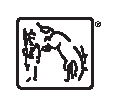
\epsfig{file=bug.eps}

\noindent
A Stata Press Publication\hfil\break
StataCorp LP\hfil\break
College Station, Texas

}
\endinput

{
\def\leftheadline{\hfil}
\def\rightheadline{\hfil}

\def\xline{\vskip-4pt\hbox to\hsize{%
\hbox{\vrule height .7pt width \hsize depth 0pt}%
}\vskip2pt}

\small

\vbox to\vsize{\vfil

\leftline{
\begin{tabular}{ll}
\multirow{3}{.5in}{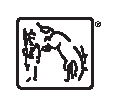
\epsfig{file=bug.eps}}&Copyright \copyright\ 2004, 2008 by
StataCorp LP\\
&All rights reserved. First edition 2004\\
&Second edition 2008\\
\end{tabular}}

\bigskip
\bigskip

\bigskip

\leftline{Published by Stata Press, 4905 Lakeway Drive, College Station, Texas 77845}

\leftline{Typeset in {\LaTeXe}}
\leftline{Printed in the United States of America}
\smallskip
\leftline{10\ \ 9\ \ 8\ \ 7\ \ 6\ \ 5\ \ 4\ \ 3\ \ 2\ \ 1}
\bigskip

\leftline{ISBN-10: !!}
\leftline{ISBN-13: !!}

\bigskip

\noindent
Library of Congress Control Number: !! 

\bigskip

\noindent
No part of this book may be reproduced, stored in a retrieval system, or
transcribed, in any form or by any means{\emdash}electronic, mechanical,
photocopy, recording, or otherwise{\emdash}without the prior written
permission of StataCorp LP.

\noindent
Stata, Mata, NetCourse, and Stata Press are registered trademarks of StataCorp
LP.  {\LaTeXe} is a trademark of the American Mathematical Society.
}

}

The acknowledgments go here.

\endinput


% Table of contents
\clearpage

\tableofcontents		% Table of contents

\listoftables			% List of tables

\listoffigures			% List of figures

\stbkpreface

\textcolor{red}{[The book introduces robust statistics in Stata from an
applied perspective. We review existing commands and present a variety of new
tools, give advice on how to choose among the different estimators and
illustrate how they can be applied in practice. After a general introduction
the book first discusses robust estimation of univariate location and scale
and, along the way, briefly introduces the basic concepts of robust statistics.
The book then moves on to simple and multiple robust regression and models for
qualitative dependent variables, each time reviewing (briefly) the theory,
presenting the algorithms, commands, and implementation details, and providing
applied examples. Furthermore, we discuss multivariate identification of
outliers and present robust versions of factor models] \dots}

% \include{version}
\stbkpreface[Notation and typography]

\subsubsection*{Stata code, datasets, programs, and references to manuals}

In this book we assume that you are somewhat familiar with \stata, that you
know how to input data and to use previously created datasets, create new
variables, run regressions, and the like. Generally, we use the \stcmd{typewriter font}
to refer to Stata commands, syntax, and variables. A “dot”
prompt followed by a command indicates that you can type verbatim what is
displayed after the dot (in context) to replicate the results in the book.

The data we use in this book are freely available for you to download, using a
net-aware Stata, from the Stata Press website,
\url{http://www.stata-press.com}. In fact, when we introduce new datasets, we
merely load them into Stata the same way that you would. For example,

\begin{stlog}
. use http://www.stata-press.com/data/!!!/football.dta, clear
\end{stlog}

\noindent
In addition, the Stata packages presented in this book may be obtained by typing

\begin{stlog}
. ssc install robstat
\oom
. ssc install robreg
\oom
. ssc install robmv
\oom
\end{stlog}

\alert{Also say what other packages need to be installed (if any), e.g. \stcmd{moremata}, I think.}

Throughout the book, we often refer to the Stata manuals using \rref{\!}, \pref{\!}, etc.
For example, \rref{regress} refers to the \textsl{Stata Reference Manual} entry for
\stcmd{regress}, and \pref{matrix} refers to the entry for \stcmd{matrix} in
the \textsl{Stata Programming Manual}.

\subsubsection*{Mathematical and statistical symbols}

We also assume that you have basic knowledge of mathematics and statistics,
although we tried to keep the exposition as simple and non-technical as
possible. Below is a list of some mathematical and statistical symbols that we
will frequently use in the book.

\begin{description}[leftmargin=6em,style=nextline]
    \item[$X, Y, Z, \dots$]
        random variables
    \item[$x_i, y_i, z_i, \dots$]
        realizations (observations) of random variables
    \item[$n$]
        number of observations
    \item[$x_{(i)}$]
        $i$th order statistic of $x_1, \dots, x_n$ ($i$th observation in the list of observations sorted in ascending order)
    \item[$F(x)$]
        cumulative distribution function of a random variable; \dots
    \item[$f(x)$]
        density \dots
    \item[$F'(x)$]
        first derivative of function $F(x)$, that is $F'(x) = dF(x)/dx = f(x)$;
        we use $'$ for both the first derivative of a function and the
        transposition of a vector or matrix
    \item[$\mathcal{N}(\mu, \sigma)$]
        normal distribution with mean $\mu$ and standard deviation $\sigma$
    \item[$\mathcal{N}(0, 1)$]
        standard normal distribution
    \item[$|x|$]
        absolute value of $x$
    \item[$\Vert\stvec{x}\Vert$]
        Euclidean norm of vector $\stvec{x} = (x_1, \dots, x_p)^t$, that is, $\Vert\stvec{x}\Vert = \sqrt{x_1^2 + \dots + x_p^2}$
    \item[$\lceil x \rceil$]
        smallest integer greater or equal to $x$
    \item[$\lfloor x \rfloor$] 
        largest integer smaller or equal to $x$
    \item[$\stvec{x}^t$, $\stmat{X}^t$]
        transposition of a vector or a matrix
    \item[\normalfont i.i.d.]
        independent and identically distributed
    \item[$\displaystyle\lim_{x\rightarrow y} g(x)$]
        limiting value of function $g(x)$ as $x$ approaches $y$
    \item[$\displaystyle\sup_x g(x)$]
        supremum (least upper bound) of function $g(x)$ with respect 
        to argument $x$
    \item[$\sign(x)$]
        the sign of $x$; to be precise, $\sign(x)=-1$ if $x<0$, $\sign(x)=+1$ if $x>0$, $\sign(x)=0$ if $x=0$
    \item[$X\sim F$]
        random variable $X$ is distributed as $F$
    \item[$X\approx F$]
        random variable $X$ is approximately distributed as $F$
    \item[\alert{...}]
        \alert{...}
\end{description}




\endinput



% File containing the chapter inserts
\clearpage
\thispagestyle{empty}
\cleardoublepage
\mainmatter
% main_inc.tex
% \include{} tex files containing \parts and \chapters here


\part{Introduction}
\label{part1}



\chapter{Introduction}
\label{chap:intro}

\section{Motivation}


Linear least-squares (\stsc{LS}) regression is, without doubt, the workhorse of
data analysis in social sciences, economics and related fields. The reasons for
the popularity of \stsc{LS} regression are obvious. The procedure convinces by
its formal and practical simplicity. \stsc{LS} regression is easy to implement
from a technical point of view and its results, the estimated regression
coefficients, are easy to interpret. Furthermore, \stsc{LS} regression is easy
to teach because its math is relatively simple and is didactically convenient
because \stsc{LS} solutions for small datasets can easily be computed manually
for purpose of exercise and understanding. From a statistical point of view,
\stsc{LS} regression is favorable because it can be shown that under the
assumption of homoscedastic (i.e., equal-variance) and normally distributed
errors the \stsc{LS} estimator is the best (i.e., most efficient) unbiased
estimator (\stsc{BUE}) for the coefficients of a linear regression model. That
is, among all possible unbiased estimators, the \stsc{LS} estimator has the
smallest sampling variance under these conditions.\footnote{Noting the
equivalence between the \stsc{LS} estimator and the arithmetic mean, the
\stsc{BUE} property of the \stsc{LS} estimator is not much of a surprise given
the fact that Carl Friedrich Gauß derived the normal distribution as a
justification for the arithmetic mean. That is, the normal distribution is
\emph{defined} as the distribution under which the \stsc{LS} procedure leads to
the best unbiased estimator for the expected value (for historical background
see \citealp{huber72}).} Also under relaxed assumption, such as non-normal or
heteroscedastic (i.e., non-equal-variance) errors, the \stsc{LS} estimator is
consistent and has, in many cases, good efficiency
properties.\footnote{Although in the later case, ordinary \stsc{LS} estimates
of the sampling variance are biased and need to be adjusted by applying
heteroscedasticity-robust variance estimation; see \citealp{white80})} For
example, in case of homoscedastic non-normal errors, the \stsc{LS} estimator is
the beast linear unbiased estimator (\stsc{BLUE}), that is, has the smallest
sampling variance among all “linear” unbiased estimators.\footnote{The term
“linear” does not refer to the fact that the coefficients of a linear
regression model are to be estimated; it refers to a property of the estimation
methodology. A linear estimators is \alert{... explain the difference between
linear and nonlinear estimators ...}}

The outstanding usefulness of \stsc{LS} regression should not be challenged
here. It is important, however, to realize that \stsc{LS} regression may not
always be the best---or at least not the only---choice for analyzing a given
dataset. The restrictiveness of the conditions under which the \stsc{LS}
estimator is deemed best---homoscedasticity and normality of errors---implies
that situations are possible in which alternative estimators can be valuable.
For example, as mentioned above, if the errors are homoscedastic but
non-normal, the \stsc{LS} estimator may be the best linear unbiased estimator,
but this also means that there can be non-linear estimators that, depending on
the nature of the deviation from normality, substantially outperform the
\stsc{LS} estimator in terms of efficiency.\footnote{The limitation to linear
estimators is not much less restrictive than the limitation to normal errors.}
In particular, in case of distributions with heavy tails, that is, if extreme
values are more frequent than in a normal distribution (an example being the
$t$-distribution with few degrees of freedom), the efficiency of the \stsc{LS}
estimator can quickly become poor. Furthermore, the \stsc{LS} estimator may
yield misleading results if the data are “contaminated” by erroneous
observations or, more generally, by a secondary data-generating process.

\paragraph{Efficiency under alternative error distributions}

Assume, for now, that the data are not contaminated and, more or less, follow a
uniform data-generating process that can be described by a linear regression
model. Why, under such a condition, can a low efficiency of the \stsc{LS}
estimator be a problem? Although, on average across multiple samples, the
\stsc{LS} estimator is unbiased, more efficient estimators would be preferable
because the precision of an estimator has a direct effect on the value of the
results. For example, the power of a significance test and, therefore, the
potential of the test to find an existing relation, decisively depends on the
efficiency of the employed estimator.

In the context of error distributions with heavy tails the efficiency argument
can also be motivated as follows. Although the \stsc{LS} estimator is unbiased
on average, there is a good chance for a single sample---and in practice often
only one sample is available---to contain extreme values that bias the
regression results in one or the other direction. Robust regression methods
that are less sensitive to such outliers will typically provide more valid
results in such situations, being closer to the true value of the parameter to
be estimated.

Figure~\ref{fig:outliers-and-fits} shows two examples of data sets that have
been generated according to model
\[
    Y = \beta_1 + \beta_2 X + \epsilon
\]
with $\beta_1 = \beta_2 = 0$ (that is, the “true” regression function is a
horizontal line at $Y=0$) and $\epsilon$ following a $t$ distribution with two
degrees of freedom, that is $\epsilon \sim t(2)$. Included as lines are the
estimated regression fits using \stsc{LS} estimation, as well as two robust
estimators (an \stsc{M} estimator and an \stsc{MM} estimator). As is evident,
the \stsc{LS} solution is affected by the outliers and suggests a positive
relation between $X$ and $Y$ in the two examples, whereas the two robust
estimator are relatively stable. Robust methods, so to say, contain a safeguard
against extreme data constellations that can occur at random due to sampling or
a stochastic data-generating process. As a diagnostic by-product, robust
methods inform about whether given data are characterized by an anomalous
constellation or not, because only in the former case the results from
\stsc{LS} and the robust methods will substantially differ.


\begin{figure}[h!]
    \centering
    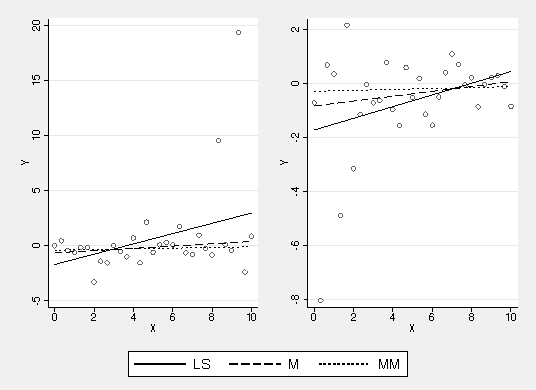
\epsfig{file=eps/2/1}
    \caption{Example scatter plots with outliers and different regression fits}
    \label{fig:outliers-and-fits}
\end{figure}

\paragraph{Bias due to data contamination}

Now assume that the data are “contaminated”, that is, that the majority of data
points follows a well-defined model, but that there are also some observations
that come from a different distribution. For example, while collecting the
data, coding errors could have occurred for some of the observations. In a
study by \citet{jasso85} on the relation between marital duration and coital
frequency there were four observations with a value of 88 for the monthly
coital frequency. Although such values would not be impossible (as argued by
\citealp{jasso85}), the observations were highly suspicious as no other values
of comparable magnitude existed in the data. As argued by \citet{kahnudry86},
the four observations probably were miscoded missing values, whose designated
value was 99. The problem with such miscoded observations is that they can have
strong effects on the results provided by a \stsc{LS} regression. That is,
regression results and the substantive conclusions drawn from them may differ
depending on whether the miscoded observations are kept in the data or not. It
seems important to use methods for data analysis that are able to identify such
problems because, in the words of \citet[18]{anscombe73}, “[w]e are usually
happier about asserting a regression relation if the relation is still apparent
after a few observations (any ones) have been deleted---that is, we are happier
if the regression relation seems to permeate all the observations and does not
derive largely from one or two.”

Conceptually, contamination can be understood as a situation in which the
observed data are the result of a mixture of two or more data-generating
processes. In the case of coding errors there may be a main process of
substantive interest (e.g., the relation between marital duration and coital
frequency), as well as a secondary process (data miscoding by interviewers)
that leads to observations that follow a different distribution and have a
different interpretation. \stsc{LS} regression will not be able to distinguish
the two processes and its results will be valid for neither one of the
processes. If, however, the data are dominated by one of the processes (that
is, if one of the processes is responsible for the bulk of the data) and the
two processes do lead to distinguishable data structures, statistical
procedures to identify the main process are possible. This is where robust
regression comes in. One of the goals of robust regression techniques is to
provide estimates that are resistant against partial contamination of the data.
Robust methods are supposed to correctly identify the primary relation in the
data even if, for example, parts of the data are glaringly erroneous.

An illustrative example comes from astronomy. Figure~\ref{fig:hrdiagram} shows
the Hertzsprung-Russell diagram of star cluster CYG OB1 (see
\citealt[27]{rousseeuw:leroy:1987}). Displayed is the logarithm of the light
intensity of the stars against the logarithm of their effective surface
temperature (using a reversed axis). Furthermore, the graph shows as lines the results of three
different regression estimators, the \stsc{LS} estimator (solid line), a low
breakdown point \stsc{M} estimator (dashed line), and a high breakdown point
\stsc{MM} estimator (dotted line). The results from the \stsc{LS} estimator and
the low breakdown point \stsc{M} estimator are almost identical. They are
strongly influenced by the group of four stars in the upper right corner of the
diagram. In contrast, the high breakdown point \stsc{MM} estimator completely
ignores the four outliers and adequately captures the trend in the main part of
the data. Hence, at least one of the two employed robust estimators
successfully identified the main process (due to the estimator's high breakdown
point; see below).


\begin{figure}[h!]
    \centering
    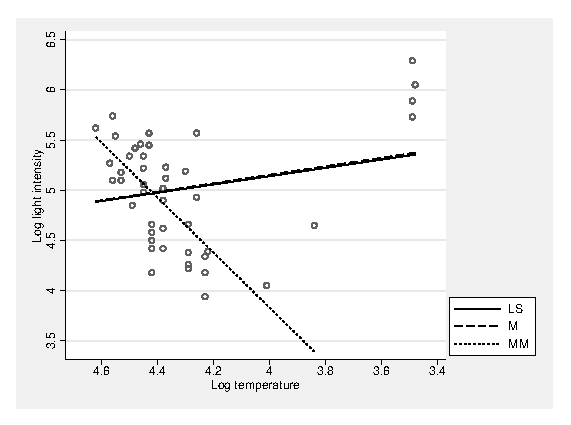
\epsfig{file=eps/2/2}
    \caption{Hertzsprung-Russell diagram of the star cluster CYG OB1 including different regression fits (source: \citealp[27]{rousseeuw:leroy:1987})}
    \label{fig:hrdiagram}
\end{figure}

Again, from a diagnostic perspective, the interesting cases are the ones in
which \stsc{LS} regression and robust estimators lead to differing results.
Substantial differences between robust regression and the \stsc{LS} estimator
indicate that the data cannot be fully descried by a uniform model and that a
part of the observations stands in stark contrast to the main trend in the
data. With the help of the residuals from robust regression, the atypical
observations can be identified and, for example, be subjected to a separate
analysis. In this way, robust regression can contribute to a better
understanding of the data and, potentially, give way to new insights and new
hypotheses. In fact, according to \citet[1]{kruskal60}, the atypical
observations may prove to be the most interesting part of the data: “An
apparently wild (or otherwise anomalous) observation is a signal that says:
`Here is something from which we may learn a lesson, perhaps of a kind not
anticipated beforehand, and perhaps more important than the main object of the
study.'” The four outliers in figure~\ref{fig:hrdiagram}, by the way, are not
errors. The explanation is that there are two different types of stars:
main-sequence stars and giants. That is, conceptually, the observation stem
from two different populations.

\paragraph{Goals and use of robust regression}

To summarize, we can state that robust regression estimators (1) should achieve
good efficiency also in case of non-normal errors and (2) should be resistant
against contamination of the data by outliers. The maximum proportion of
contamination a robust estimator is able to absorb is called the
\emph{breakdown point}.

Both aspects can be formalized with the help of the viewpoint coined by 
\citet{huber64} that observed data follow a mixture distribution
\[
    F_\varepsilon = (1 - \varepsilon) F_{\boldsymbol\theta} + \varepsilon G
\]
where $F_{\boldsymbol\theta}$ is the distribution of interest according to the
supposed model, $G$ is an arbitrary alternative distribution, and $\varepsilon
\in [0,1]$ determines the mixing proportion. For example, in line with the
assumptions of classic linear regression, $F_{\boldsymbol\theta}$ could be a
distribution according to the linear model
\[
    Y = \beta_1 + \beta_2 X + \dots + \epsilon
\]
where $X$ has a given distribution and $\epsilon$ is an independent and
identically normally distributed error term. The distribution of the observed
data, however, is contaminated by observations from an unspecified alternative
distribution $G$ and does not fully follow this model. The goal of robust
regression now is to deliver reasonable results for $F_{\boldsymbol\theta}$
even if the model is somewhat misspecified, that is, if $\varepsilon>0$. In the
words of \citet[7]{heritier.etal.09}, robust methods are “a set of statistical
tools for correct estimation and inference about $F_\theta$ when the
data-generating process is $F_\varepsilon$, not only when $\varepsilon=0$, as
with classical methods, but also for relatively small $\varepsilon$ and
\emph{any} $G$. As a by-product, data not fitting $F_\theta$ exactly can be
easily identified, and the model can possibly be changed and refitted.“ In
addition, to be of diagnostic value, robust estimators should be serious
competitors of classic methods in case of $\varepsilon=0$. In particular,
robust estimators should achieve good “gaussian efficiency”, that is, they
should achieve a hight relative efficiency compared to \stsc{LS} estimation in
the ideal case of normally distributed errors.\footnote{Note that the
estimation of “robust standard errors” is not the primary concern of robust
regression. The term “robust standard errors” refers to estimators for the
sampling variances of the coefficient estimates that are consistent also if the
assumption of identically distributed errors is violated (i.e., if the errors
are heteroscedastic; see \citealp{white80}). To prevent false conclusions with
respect to confidence intervals and significance tests, it is always a good
idea to consider “robust standard errors”, be it with classic regression or
with robust regression.}

Yet, robust regression should be seen as a complement and not so much as a
substitute to \stsc{LS} regression. In our view, the main use of robust
regression lies in its diagnostic potential. Classic regression techniques may
lead to meaningful results in many situations, but a comparison to robust
results is always advisable. Before drawing far-reaching conclusions based on
classic methods one should evaluate whether the conclusions are “robust”, that
is, whether methods that rely on less restrictive assumptions and are less
affected by outliers and atypical data constellations come to the same
conclusions.

If classic procedures and robust regression lead to substantially diverging or
even contradicting results, the robust results can provide an immediate
contribution to a better understanding of the data. As a by-product of robust
estimation, observations that do not fit the supposed model can easily be
identified, offering clues about possible misspecification, the nature of
outliers, and alternative data-generating processes. Compared to classic
regression diagnostics for the identification of influential observations (see
\citealp{belsley80,cookweisberg82,Chatterjee88,fox91}) robust regression
methods have the advantage that they can also identify “masked” multiple
outliers that would go undetected by classic diagnostics. However, robust
techniques are no panacea and cannot, for example, fully replace diagnostic
methods that are concerned with the identification of structural
misspecification (such as omitted variable bias, wrong functional form, or
missing interaction terms).



\alert{
[Should there also be some text giving a brief historical account of the development 
of robust statistics and robust regression?]
}


\section{What is covered in this book?}

\alert{
\dots
}


\section{Robust statistics in Stata}

\alert{
\begin{itemize}
    \item
    Summary of existing tools
    \item
    Brief presentation of our new packages; basic usage and syntax
\end{itemize}
}


\endinput
  % Introduction

\part{Robustness theory and basic robust statistics}
\label{part2}




\chapter{Basic concepts in estimation}
\label{chap:theory}

An estimation problem in statistics may have many potential solutions. To
separate useful estimation strategies from approaches that are less feasible,
criteria have to be defined by which different estimators can be evaluated and
compared. In this chapter we first review a number of basic criteria typically
used in classic statistics. We then discuss additional criteria that are
important in the context of robust statistics. Our discussion in this chapter
is conceptual in nature; it is supposed to establish a theoretical basis for
the specific robust estimators that are discussed in the subsequent chapters
from an applied perspective.

\section{Classical properties of estimators}

The goal of statistical estimation is to obtain a reasonable value for the
unknown \emph{paramater} of a statistical model, based on data whose properties
are assumed to be consistent with the suggested model. Let $\mathcal{X}^{(n)} =
\{X_1, \dots, X_n\}$ be a set of $n$ random variables $X_1, \ldots, X_n$ that
have a joint probability distribution $P_{\boldsymbol\theta}^{(n)}$ depending
on the unknown parameter $\boldsymbol\theta$. Note that, depending on context,
$\boldsymbol\theta$ may be scalar, or it may be a vector of multiple
parameters, that is $\boldsymbol\theta = (\theta_1, \dots, \theta_p)^t$. For
simplicity, we consider here that the observations $X_i$ are univariate.
However, the concepts introduced hereafter may be (quite easily) generalized in
the case of multivariate observations $\stvec{X}_i$, that is, in the case
$\stvec{X}_i$ is a vector of random variables
($\stvec{X}_i=(X_{i1},\ldots,X_{ik})^t$).

Since $\boldsymbol\theta$ is unknown, this actually leads to assume that the
joint distribution of the random variables $X_i$, $i=1, \dots, n$, belongs to
the (parametric) \emph{statistical model} $\mathcal{P}^{(n)} =
\{P_{\boldsymbol\theta}^{(n)} | \boldsymbol\theta \in \boldsymbol\Theta\}$,
where $\boldsymbol\Theta$ is the set of possible values of $\boldsymbol\theta$.
The goal is to estimate $\boldsymbol\theta \in \boldsymbol\Theta$ based on a
realization of $\mathcal{X}^{(n)}$. In general, we will consider the case in
which the statistical model $\mathcal{P}^{(n)}$ conforms to simple random
sampling (\stsc{SRS}), that is, a situation in which the random variables $X_1,
\dots, X_n$ are independent and identically distributed (i.i.d.). In this
situation, each $X_i$ independently follows a common probability distribution
$P_{\boldsymbol\theta}$, which can be characterized by the distribution
function $F_{\boldsymbol\theta}(\stvec{x}) = \Pr(X_i \leq x)$ (or simply $F$
when there is no risk of confusion about the parameter we have to estimate).

An \emph{\Index{estimator}} of $\boldsymbol\theta$ can then be defined as
follows: An \Index{estimator} of the parameter $\boldsymbol\theta$ is any
statistic $\sthat{\boldsymbol\theta} =
\sthat{\boldsymbol\theta}(\mathcal{X}^{(n)})$ taking its value in
$\boldsymbol\Theta$.

The value of $\sthat{\boldsymbol\theta}$ provided by a particular realization
$x_1,\ldots,x_n$ of the random variables $X_1, \dots, X_n$ is called an
\emph{\Index{estimate}} of $\boldsymbol\theta$. Note that, for simplicity, we
will often use the notation $x_i$ ($i \in \{1, \dots, n\}$) to designate the
$i$th random observation as well as a realization of it (i.e., a specific
value); the context will always clearly indicate if we have to consider $x_i$
as a random variable or as a particular value.

The definition above contains no indication of the quality of an estimator; any
statistic $\sthat{\boldsymbol\theta}$ that provides a value in
$\boldsymbol\Theta$ is a valid estimator. To narrow down the set of estimators
to estimators that can be considered useful we need quality criteria. Classic
quality criteria are unbiasedness, efficiency, and consistency.

\subsection{Unbiasedness}
\Index[unbiasedness]{}

From a good estimator one may expect that, on average, it gives the “correct”
answer. Let us denote by
$E_{\boldsymbol\theta}(\sthat{\boldsymbol\theta}(\mathcal{X}^{(n)}))$ the
expectation of statistic $\sthat{\boldsymbol\theta}(\mathcal{X}^{(n)})$ when
$\mathcal{X}^{(n)} \sim P_{\boldsymbol\theta}^{(n)}$. Think of
$E_{\boldsymbol\theta}$ as the average value we would obtain for
$\sthat{\boldsymbol\theta}$ from a large number of repeated realizations of
$\mathcal{X}^{(n)}$, given that for each repetition $\mathcal{X}^{(n)}$ follows
distribution $P_{\boldsymbol\theta}^{(n)}$ (as, for example, in repeated random
sampling from the same population).

Unbiasedness can then be defined as follows:
The estimator $\sthat{\boldsymbol\theta} = \sthat{\boldsymbol\theta} 
(\mathcal{X}^{(n)})$ is called unbiased if
\[
    E_{\boldsymbol\theta}(\sthat{\boldsymbol\theta}) = \boldsymbol\theta
    \qquad
    \text{for all $\boldsymbol\theta \in \boldsymbol\Theta$ and all $n$}.
\]

That is, no matter the sample size $n$, estimator $\sthat{\boldsymbol\theta}$
will, on average across a large number of repeated samples, provide the correct
value of $\boldsymbol\theta$ (given that our assumptions about the joint distribution of
$\mathcal{X}^{(n)}$ are correct, such as, e.g., independent sampling of
observations). The difference
\[
    B_{\boldsymbol\theta}(\sthat{\boldsymbol\theta}) 
        = E_{\boldsymbol\theta}(\sthat{\boldsymbol\theta}) - \boldsymbol\theta
\]
is called the \emph{\Index{bias}} of estimator $\sthat{\boldsymbol\theta}$.
The absence of bias indicates that the sampling distribution of
$\sthat{\boldsymbol\theta}$ has a mean that coincides with the value of the
parameter of interest.

Zero bias is often difficult to achieve in small samples. Therefore, another
useful criterion is \emph{asymptotic unbiasedness}: The estimator
$\sthat{\boldsymbol\theta} = \sthat{\boldsymbol\theta}(\mathcal{X}^{(n)})$ is
called asymptotically unbiased if
\[
    \lim_{n \rightarrow \infty} E_{\boldsymbol\theta}(\sthat{\boldsymbol\theta}) = \boldsymbol\theta
    \qquad
    \text{for all $\boldsymbol\theta \in \boldsymbol\Theta$}.
\]

That is, an estimator is asymptotically unbiased if the bias vanishes with 
increasing sample size. An important question in this context is, of course, how 
fast the bias vanishes (or how large the sample size has to be for the bias to be 
negligible).

\subsection{Efficiency}

For a specific estimation problem, several (asymptotically) unbiased estimators
may exist. To choose the best among them we need further information about the
performance of the different estimators. Furthermore, there may also be
situations in which a biased estimator is to be preferred over an unbiased
estimator. A key aspect in this regard is the \emph{\Index{efficiency}} of an
estimator. Efficiency has to do with how spread out about $\boldsymbol\theta$
the sampling distribution of the estimator is. The smaller the dispersion of
estimator $\sthat{\boldsymbol\theta}$ around the true value
$\boldsymbol\theta$ in repeated samples, the more “efficient” (or precise) is
the estimator.

\paragraph{Mean squared error}

First consider the case of a \emph{scalar} parameter $\theta$. The
precision of estimator $\sthat{\theta}$ can be measured by its
\emph{\Index{mean squared error}} (\stsc{MSE}):
\[
    \stsc{MSE}_{\theta}(\sthat{\theta}) 
    = E_{\theta} \left((\sthat{\theta} - \theta)^2\right).
\]
A small mean squared error for $\sthat{\theta}$ means that the sampling
distribution of $\sthat{\theta}$ is well concentrated around the exact value
of the parameter to estimate and hence that the estimator $\sthat{\theta}$
has a good precision.

It is easy to show that
\[
    \stsc{MSE}_{\theta}(\sthat{\theta})
    = \mathrm{Var}_{\theta}(\sthat{\theta}) 
      + \left(B_{\theta}(\sthat{\theta})\right)^2.
\]
That is, the mean squared error of an estimator can be decomposed into its
variance and its squared bias. Hence, if $\sthat{\theta}$ is unbiased,
$\stsc{MSE}_{\theta}(\sthat{\theta})$ is simply equal to
$\mathrm{Var}_{\theta}(\sthat{\theta})$.

\paragraph{Relative efficiency}

An estimator $\sthat{\theta}_A$ of $\theta$ is more precise---we will say
\emph{more efficient}---than another estimator $\sthat{\theta}_B$ if
\[
    \stsc{MSE}_{\theta}(\sthat{\theta}_A) \leq 
    \stsc{MSE}_{\theta}(\sthat{\theta}_B)
    \qquad\text{for all $\theta \in \Theta$}
\]
and
\[
    \stsc{MSE}_{\theta}(\sthat{\theta}_A) < 
    \stsc{MSE}_{\theta}(\sthat{\theta}_B)
    \qquad\text{for at least one $\theta \in \Theta$}.
\]


In general, we consider the “large-sample” sampling distributions of
asymptotically unbiased estimators. If, for large $n$, the estimators
$\sthat{\theta}_A$ and $\sthat{\theta}_B$ are approximately
$\mathcal{N}(\theta, \textrm{Var}(\sthat{\theta}_A))$ and
$\mathcal{N}(\theta, \textrm{Var}(\sthat{\theta}_B))$, respectively, we
define the \emph{\Index{asymptotic relative efficiency}} (\stsc{ARE}) of
$\sthat{\theta}_B$ with respect to $\sthat{\theta}_A$ as the ratio
\[
    \stsc{ARE}_{\theta}(\sthat{\theta}_B,\sthat{\theta}_A) 
    = \frac{ \textrm{Var}(\sthat{\theta}_A)}{\textrm{Var}(\sthat{\theta}_B)}
\]
(see \citealp{Serfling1980}). If $\sthat{\theta}_B$ is (asymptotically) less
efficient than $\sthat{\theta}_A$, then
\[
    \stsc{ARE}_{\theta}(\sthat{\theta}_B,\sthat{\theta}_A) \leq 1
\]
for all $\theta \in \Theta$, with strict inequality holding for at least some
value of $\theta$.


\paragraph{Efficiency of the maximum likelihood estimator}

Let us consider the case in which the random variables $X_1, \ldots, X_n$ of
the sample ${\cal X}^{(n)}$ are i.i.d.\ with a common distribution function
$F_{\theta}$ and a common density function $f_{\theta}$ that satisfies some
differentiability conditions with respect to $\theta$. Suppose also that the
\emph{\Index{Fisher information}}
\[
    \mathcal{I}\left(F_{\theta}\right) =
        E_{\theta}\left(\left(\frac{\partial}{\partial\theta}
        \log f_{\theta}(X)\right)^2\right)
\] 
is strictly positive and finite. Then it follows that
\begin{enumerate}
    \item[(i)] for large $n$, the maximum likelihood estimator
    $\sthat{\theta}_{\stsc{ML}}$ of $\theta$ is approximately distributed as
    $\mathcal{N}\left(\theta, (n \mathcal{I}(F_{\theta}))^{-1}\right)$
    
    \item[(ii)] for a wide class of estimators $\sthat{\theta}$ that are
    approximately distributed as $\mathcal{N}(\theta, V)$, a \emph{lower
    bound} to $V$ is $(n \mathcal{I}(F_{\theta}))^{-1}$
\end{enumerate}
(see \citealp{LehmannCasella1988}). In this situation,
%
\begin{equation}\label{eq:ARE_vsML}
    \stsc{ARE}_{\theta}(\sthat{\theta}, \sthat{\theta}_{\stsc{ML}})
     = \frac{(n \mathcal{I}(F_{\theta}))^{-1}}{V} \leq 1
\end{equation}
%
for all $\theta \in \Theta$, making $\sthat{\theta}_{\stsc{ML}}$ the most
(asymptotically) efficient among the given class of estimators
$\sthat{\theta}$. Note, however, as will be discussed later, that
(\ref{eq:ARE_vsML}) does not necessarily make $\sthat{\theta}_{\stsc{ML}}$ the
estimator of choice, when certain other considerations are taken into account.


\paragraph{Notation in the multidimensional case}

If $\boldsymbol\theta = (\theta_1, \dots, \theta_p)^t$ is a vector of parameters
we define the \emph{\Index[mean squared error!matrix]{mean squared error matrix}}
of the estimator $\sthat{\boldsymbol\theta}$ as follows:
\[
    \stsc{MSE}_{\boldsymbol\theta}(\sthat{\boldsymbol\theta})
    = E_{\boldsymbol\theta}\left((\sthat{\boldsymbol\theta} - \boldsymbol\theta)
                                 (\sthat{\boldsymbol\theta} - \boldsymbol\theta)^t
                           \right).
\]
If $\sthat{\boldsymbol\theta}$ is unbiased, the mean squared error matrix simply
coincides with the covariance matrix of the estimator.

If, for large $n$, the $p$-variate estimators $\sthat{\boldsymbol\theta}_A$ and
$\sthat{\boldsymbol\theta}_B$ are approximately normally distributed with mean
$\boldsymbol\theta$ and nonsingular covariance matrices $\boldsymbol\Sigma_A$ and
$\boldsymbol\Sigma_B$, respectively, it is usual to define the 
\emph{\Index{asymptotic relative efficiency}} (\stsc{ARE}) of
$\sthat{\boldsymbol\theta}_B$ with respect to $\sthat{\boldsymbol\theta}_A$ as
the ratio of the \emph{generalized variances} (determinants of the covariance
matrices), raised to the power $1/p$, that is
\[
    \stsc{ARE}_{\boldsymbol\theta}(\sthat{\boldsymbol\theta}_B, \sthat{\boldsymbol\theta}_A)
    = \left(\frac{ \det(\boldsymbol\Sigma_A)}{\det(\boldsymbol\Sigma_B)}\right)^{1/p}.
\]
If $\stsc{ARE}_{\boldsymbol\theta}(\sthat{\boldsymbol\theta}_B,
\sthat{\boldsymbol\theta}_A) \leq 1$ for all $\boldsymbol\theta \in
\boldsymbol\Theta$, with strict inequality holding for at least some value
$\boldsymbol\theta$, estimator $\sthat{\boldsymbol\theta}_B$ is
(asymptotically) less efficient than estimator $\sthat{\boldsymbol\theta}_A$.

Here again the maximum likelihood estimator $\sthat{\boldsymbol\theta}_\stsc{ML}$ of
$\boldsymbol\theta$ appears as the most (asymptotically) efficient estimator among a
wide class of (asymptotically) unbiased estimators $\sthat{\boldsymbol\theta}$ of
$\boldsymbol\theta$. Moreover, for large $n$,
\[
    \sthat{\boldsymbol\theta}_\stsc{ML} \approx 
    \mathcal{N}\left(\boldsymbol\theta, (n \stmat{I}(F_{\boldsymbol\theta}))^{-1}\right)
\]
where “$\approx$” stands for “is approximately distributed as” and
$\stmat{I}(F_{\boldsymbol\theta})$ is the $p\times p$ Fisher information matrix
with its elements defined as
\[
    \mathcal{I}_{ij}\left(F_{\boldsymbol\theta}\right) =
    E_{\boldsymbol\theta}\left(
    \frac{\partial}{\partial\theta_i}\log f_{\boldsymbol\theta}(X) \times 
    \frac{\partial}{\partial \theta_j}\log f_{\boldsymbol\theta}(X)
    \right).
\] 


\subsection{Consistency}
\Index[consistency]{}

High efficiency and (asymptotic) unbiasedness are desired properties for an
estimator. But other properties are still required if we want the estimator to
provide valid statistical inference for $\boldsymbol\theta$.

The sampling distribution of $\sthat{\boldsymbol\theta}$ generally depends on
the size $n$ of the sample, e.g. via its mean, its variance and (or) other
characteristics. How does the distribution of $\sthat{\boldsymbol\theta}$
evolve when $n$ increases? This question will first lead us to the properties
of \emph{(asymptotic) consistency} ---\emph{convergence in probability}--- and
\emph{Fisher consistency}. We will then consider the concept of
\emph{convergence in distribution}.

\paragraph{(Asymptotic) consistency: Convergence in probability}
\Index[convergence!in probability]{}
\Index[consistency!asymptotic]{}

An estimator $\sthat{\boldsymbol\theta} =
\sthat{\boldsymbol\theta}(\mathcal{X}^{(n)})$ is \emph{consistent} or
\emph{asymptotic consistent} if, for $n \rightarrow \infty$,
$\sthat{\boldsymbol\theta}$ \emph{converges in probability} to
$\boldsymbol\theta$. That is, for any $\epsilon > 0$ and for all
$\boldsymbol\theta \in \boldsymbol\Theta$:
\begin{equation}
    \lim_{n \rightarrow \infty} P_{\boldsymbol\theta}^{(n)} \left(
        \Vert\sthat{\boldsymbol\theta} - \boldsymbol\theta \Vert \leq \epsilon
        \right) = 1. \label{eq:consistency}
\end{equation}

This type of convergence means that, when the sample size grows, the
probability that the estimator $\sthat{\boldsymbol\theta}$ takes a value
arbitrarily close to the exact value of the parameter and, consequently,
provides a “good” estimate of the parameter $\boldsymbol\theta$, grows to 1.

In other terms, a consistent estimator $\sthat{\boldsymbol\theta}$ of
$\boldsymbol\theta$ is an estimator that becomes more and more precise when the
number of observations increases. It also means that the sampling distribution
of $\sthat{\boldsymbol\theta}$ becomes more and more concentrated around the
true value of the parameter being estimated. This property of consistency is of
course a highly desirable property for an estimator.

\paragraph{Convergence in quadratic mean}
\Index[convergence!in quadratic mean]{}

Another type of convergence is closely related to the notion of consistency:
the \emph{convergence in quadratic mean}. For simplicity, consider the case of
a scalar parameter $\theta$: $\sthat{\theta}=\sthat{\theta}({\cal X}^{(n)})$
converges in quadratic mean to $\theta$ if
\[
    \stsc{MSE}_{\theta}(\sthat{\theta})=E_{\theta}\left((\sthat{\theta}-\theta)^2\right) 
    \stackrel{n \rightarrow \infty}{\longrightarrow} 0.
\]

Since $\stsc{MSE}_{\theta}(\sthat{\theta})={\rm Var}_{\theta}(\sthat{\theta}) +
\left(B_{\theta}(\sthat{\theta})\right)^2$, it is clear that, if
$\sthat{\theta}$ is asymptotically unbiased and has a variance that tends to
zero when $n$ tends to infinity, then $\sthat{\theta}$ converges to $\theta$ in
quadratic mean. Moreover, it is quite easy to prove that the convergence in
quadratic mean implies the convergence in probability. This result is intuitive
since $\stsc{MSE}_{\theta}(\sthat{\theta})$ is nothing but a measure of the
dispersion of the sampling distribution of $\sthat{\theta}$ around the exact
value of the parameter to estimate.

In practice, it is often easier to establish the consistency of
$\sthat{\theta}$ by verifying that $\sthat{\theta}$ converges in quadratic mean
to $\theta$ instead of considering directly the equality (\ref{eq:consistency}).

\paragraph{Fisher consistency}
\Index[consistency!Fisher]{}

In statistics, \emph{Fisher consistency} is another desirable property of an
estimator asserting that if the estimator were calculated using the entire
population rather than a sample, the true value of the estimated parameter
would be obtained (\citealp{fisher:1922}).

Suppose we have a statistical sample ${\cal X}^{(n)}=\{X_1,\ldots,X_n\}$ where
each $X_i$ has a distribution characterized by the cumulative distribution
$F_{\boldsymbol\theta}$ which depends on an unknown parameter
$\boldsymbol\theta$. If the estimator
$\sthat{\boldsymbol\theta}=\sthat{\boldsymbol\theta}({\cal X}^{(n)})$ can be
represented as a \emph{functional} of the empirical distribution
function\footnote{The empirical distribution function $F^{(n)}$ is the
distribution function associated with the discrete probability distribution
allocating a probability mass of $1/n$ at each observation $X_i$,
$i=1,\ldots,n$, of the sample ${\cal X}^{(n)}$.} $F^{(n)}$, that is,
\[
    \sthat{\boldsymbol\theta}=\stvec{T}(F^{(n)}),
\] 
$\sthat{\boldsymbol\theta}$ is said to be \emph{Fisher consistent} if
\[
    \stvec{T}(F_{\boldsymbol\theta})=\boldsymbol\theta .
\]

If the strong law of large numbers can be applied, the empirical distribution
function $F^{(n)}$ converges pointwise to $F_{\boldsymbol\theta}$ when $n$
tends to infinity, allowing us to express Fisher consistency as the following
convergence property: The estimator
$\sthat{\boldsymbol\theta}=\stvec{T}(F^{(n)})$ is Fisher consistent if
\[
    \stvec{T}\left(\lim_{n\rightarrow\infty} F^{(n)}\right)=\boldsymbol\theta .
\] 

Fisher consistency and (asymptotic) consistency are distinct concepts, although
both aim to define a desirable property of an estimator. While many estimators
are consistent in both senses, neither definition encompasses the other: There
exist estimators that are (asymptotically) consistent but not Fisher consistent
and, inversely, there are estimators that are Fisher consistent but not
(asymptotically) consistent.

\subsection{Convergence in distribution}
\Index[convergence!in distribution]{}

A last type of convergence is important when we have to provide a confidence
interval for (each component of) $\boldsymbol\theta$ or to define a statistical
test to solve a testing problem for the unknown parameter $\boldsymbol\theta$:
The \emph{convergence in distribution}. Since this property concerns usually a
function of an estimator $\sthat{\boldsymbol\theta}$ of $\boldsymbol\theta$
than the estimator $\sthat{\boldsymbol\theta}$ itself, we formulate it in a
general way for a statistic $\stvec{U}^{(n)}=\stvec{U}({\cal X}^{(n)})$.

The statistic $\stvec{U}^{(n)}$ \emph{converges in distribution} to the
probability distribution ${\cal L}$ if, for $n \rightarrow \infty$, the
distribution function $F_{\stvec{U}^{(n)}}$ of $\stvec{U}^{(n)}$ converges to
the distribution function $F_{\cal L}$ associated with ${\cal L}$ in any point
of continuity of $F_{\cal L}$. That is, convergence in distribution is given if
\[
    F_{\stvec{U}^{(n)}}(\stvec{u}) \stackrel{n \rightarrow \infty}{\longrightarrow} F_{\cal L}(\stvec{u})
\] 
for any continuity point $\stvec{u}$ of the distribution function $F_{\cal L}$.

As a shorthand, we will write
\[
    \stvec{U}^{(n)} \stackrel{d}{\rightarrow} \mathcal{L}
\]
to denote convergence in distribution for $n \rightarrow \infty$. In practice, 
convergence in distribution means that, for large $n$, we may consider that
$\stvec{U}^{(n)}$ is approximately distributed as $\mathcal{L}$, that is,
\[
    \stvec{U}^{(n)} \approx \mathcal{L}.
\]

In practice, it is useful to consider an estimator $\sthat{\boldsymbol\theta}$
of $\boldsymbol\theta$ such that a certain function of
$\sthat{\boldsymbol\theta}$ converges in distribution to a well known
probability distribution ${\cal L}$ as, for example, a normal distribution, a
Student distribution, a chi-square or a Fisher distribution. Indeed it allows
to develop inference procedures for $\boldsymbol\theta$, based on
$\sthat{\boldsymbol\theta}$, that are valid when the sample size $n$ is not too
small.

\subsection{Other aspects}

Depending on context, a number of other criteria can be important. For example,
from a practical perspective, \emph{computational complexity} can be a relevant
criterion to choose between different estimators. In general, estimators that
require operations in the order of $n^2$ (that is, if the number of required
computational operations grows quadratically with the sample size) lead to
prohibitive computational costs in large samples. In many cases it is possible
to design alternative estimators (or improved computational algorithms
for a given estimator) that only require operations in the order of $\ln n$ and
are thus much more efficient (with respect to computer time) in large samples.
\alert{[Maybe expand a bit on this.]}

Furthermore, consistent estimators may differ in their \emph{rate of
convergence}, that is, in how fast the mean squared error diminishes with
growing sample size. 

If $\stsc{MSE}_{\boldsymbol\theta}(\sthat{\boldsymbol\theta})$ is of order
$n^{-\nu}$ (with $\nu > 0$ such that the mean squared error of
$\sthat{\boldsymbol\theta}$ tends to zero when $n$ tends to infinity, ensuring
the convergence of $\sthat{\boldsymbol\theta}$ in quadratic mean and, hence, in
probability), the rate of convergence of $\sthat{\boldsymbol\theta}$ is said to
be equal to $n^{\nu/2}$. This rate of convergence is actually the factor by
which we have to multiply $\sthat{\boldsymbol\theta}$ to obtain a mean squared
error that does not depend anymore on the sample size $n$. Most of estimators
in parametric models have a mean squared error of order $n^{-1}$ and,
consequently, enjoy a rate of convergence equal to $\sqrt{n}$. It is the case,
for example, for the least squares estimator of the regression coefficients
vector in the classical linear regression model. The squared root of $n$ is
certainly considered as the usual rate of convergence in the parametric
context. In the nonparametric context, we may encounter estimators whose rate
of convergence is smaller than $\sqrt{n}$. This is the case, for instance, for
a kernel estimator of a density function $f$: The kernel estimator of $f(x)$
has a mean squared error of order $n^{-4/5}$ and hence a rate of convergence
equal to $n^{2/5}$.

Naturally, an estimator with a faster rate of convergence is usually to be
preferred over an estimator with a slower rate of convergence.

Finally, an estimator should be \emph{equivariant} to transformations of data.
That is, a transformation of the data should affect the estimator
$\sthat{\boldsymbol\theta}$ in the same functional way as it affects the true
parameter $\boldsymbol\theta$. For example, let $\theta_A$ be the expected
value of variable $X_A$ and $\theta_B$ be the expected value of variable $X_B$.
If $X_B$ can be expressed as a linear combination of $X_A$, that is, $X_B = a +
b X_A$, then $\theta_B = a + b \theta_A$. In this case, also
$\sthat{\theta}_B = a + b \sthat{\theta}_A$ should hold. In other words,
whether you express your data in Dollars or in Euros, whether you express your
data in degrees Fahrenheit or degrees Celsius should only affect the scaling of
your estimator, but should not affect your results otherwise.


\section{Measures of robustness}

Intuitively, the classical approach to statistics is about defining estimators
that have desirable properties under a specified model. The goal of
robust methods, however, is to develop estimators that perform well also in the
“neighborhood” of such a model. This leads to the proposition of so called
“robust” estimators, that are, for instance, not affected too strongly or too
quickly by the presence of outliers. Although outliers are only one of
the main concerns of robust methods, we will make our first steps into
robustness theory by presenting some basic concepts for measuring the degree to
which estimators are affected by atypical observations.


\begin{stexample}
    Consider the following observations of the grades achieved by $n = 25$ students
    in fifth year of primary school (on a scale of 0 to 10):                       
    
    \begin{center}
    \begin{tabular}{rrrrrr}%
    6.00 & 6.50 & 7.00 & 7.00 & 7.00\\
    7.00 & 7.00 & 7.50 & 7.50 & 8.00\\
    8.00 & 8.00 & 8.50 & 8.50 & 8.50\\
    8.50 & 9.00 & 9.00 & 9.50 & 9.50\\
    9.50 & 9.50 & 9.50 & 9.50 & 10.00
    \end{tabular}
    \end{center}
    
    If we calculate on these data two \emph{measures of location}, the \Index{mean} and the
    \Index{median}, as well as two \emph{measures of scale}, the
    \Index{standard deviation} and the \Index{interquartile range}, the results
    are as follows:
    
\begin{stlog}
. drop _all
{\smallskip}
. matrix x = (6.00, 6.50, 7.00, 7.00, 7.00,    ///
>             7.00, 7.00, 7.50, 7.50, 8.00,    ///
>             8.00, 8.00, 8.50, 8.50, 8.50,    ///
>             8.50, 9.00, 9.00, 9.50, 9.50,    ///
>             9.50, 9.50, 9.50, 9.50, 10.00)'
{\smallskip}
. quietly svmat x
{\smallskip}
. tabstat x, statistics(mean median sd iqr)
{\smallskip}
    variable {\VBAR}      mean       p50        sd       iqr
\HLI{13}{\PLUS}\HLI{40}
          x1 {\VBAR}      8.22       8.5  1.137248       2.5
\HLI{13}{\BOTT}\HLI{40}
{\smallskip}

\end{stlog}
    
    Now, imagine the dot separating the decimals in the last observation is
    mistakenly removed, so that the last observation is coded as 1000. In this 
    case the results are the following:
    
\begin{stlog}
. use Star.dta, clear
{\smallskip}
. regress log_intensity log_temperature
{\smallskip}
      Source {\VBAR}       SS           df       MS      Number of obs   =        47
\HLI{13}{\PLUS}\HLI{34}   F(1, 45)        =      2.08
       Model {\VBAR}  .664593334         1  .664593334   Prob > F        =    0.1557
    Residual {\VBAR}  14.3463934        45  .318808743   R-squared       =    0.0443
\HLI{13}{\PLUS}\HLI{34}   Adj R-squared   =    0.0230
       Total {\VBAR}  15.0109868        46  .326325799   Root MSE        =    .56463
{\smallskip}
\HLI{14}{\TOPT}\HLI{64}
log_intensity {\VBAR}      Coef.   Std. Err.      t    P>|t|     [95\% Conf. Interval]
\HLI{14}{\PLUS}\HLI{64}
log_tempera{\tytilde}e {\VBAR}  -.4133041   .2862575    -1.44   0.156    -.9898562     .163248
        _cons {\VBAR}   6.793468   1.236516     5.49   0.000     4.302998    9.283939
\HLI{14}{\BOTT}\HLI{64}
{\smallskip}

\end{stlog}
    
    As is evident, the \Index{mean} and the \Index{standard deviation} strongly
    increased due to the introduction of the erroneous observation, whereas
    the \Index{median} and the \Index{interquartile range} remained unchanged.
    The example illustrates the fact that one single outlier may “break” the
    \Index{mean} and the \Index{standard deviation}, but does not affect the
    \Index{median} or the \Index{interquartile range}. Hence, these two later
    statistics can be considered as being more robust to erroneous data than
    the two first ones.

\end{stexample}

How can the degree of robustness of different statistics be quantified? How can
we compare the robustness of different estimators from various viewpoints?
These are questions we will address in the rest of this section.

In robust estimation theory it is common to consider \emph{parameters} as
\emph{functionals}. More precisely, the functional by which a
parameter\footnote{For the sake of simplicity, we will only consider here
\emph{scalar} parameters.} $T$ is defined is a rule that maps every
distribution function $F$ into a real number, that is, $T = T(F)$.\footnote{$F$
is the cumulative distribution function of a random variable $X$. Evaluated at
position $x$, the function returns the probability that the random variable
will take on a value lower than or equal to $x$, that is, $F(x) = \Pr(X \leq
x)$. In order to avoid unnecessary technical difficulties we will generally
assume in this chapter that the distribution $F$ is continuous with density
$f$. The density is the first derivative of $F$; it is nonnegative and
integrates to one.} Often, a natural \emph{estimate} $T^{(n)}$ of the parameter
$T(F)$ based on sample ${\mathcal X}^{(n)}= \{x_1, \dots, x_n\}$---where $x_1,
\dots, x_n$ are realizations of $n$ independent and identically distributed
(i.i.d.) random variables $X_1, \dots, X_n$ of distribution $F$---may be
defined as the value of the functional at the empirical distribution
$F^{(n)}$.\footnote{The empirical distribution function $F^{(n)}$ is the
distribution function associated with the discrete probability distribution
allocating a probability mass of $1/n$ at each observation $x_i$,
$i=1,\ldots,n$, of the sample ${\mathcal X}^{(n)}$.} That is, $T^{(n)} =
T(F^{(n)})$. For example, if
\[
    T(F) = \int_{-\infty}^\infty x \dif F(x) = \mu
\]
is the expected value of the distribution $F$, then
\[
    T^{(n)} = T(F^{(n)}) = \int_{-\infty}^\infty x \dif F^{(n)}(x) 
          = \frac{1}{n} \sum_{i=1}^n x_i = \mu^{(n)}
\]
is the arithmetic \Index{mean} of a sample ${\mathcal X}^{(n)}$ from $F$.
Likewise, if $T(F) = F^{-1}(0.5) = Q_{0.5}$ is the \Index{median} of the
distribution $F$, then $T^{(n)} = T(F^{(n)}) = (F^{(n)})^{-1}(0.5) =
Q_{0.5}^{(n)}$ is the empirical median of a sample ${\cal X}^{(n)}$ from $F$.

The robustness of a statistic (or estimator) $T^{(n)}$ may be analyzed in a very
intuitive way by studying how a contamination of the sample
$\mathcal{X}^{(n)}$ affects $T^{(n)}$. This empirical approach leads to the notions of
the \emph{\Index{sensitivity curve}} and the \emph{\Index[breakdown
point!finite-sample]{finite-sample breakdown point}} of $T^{(n)}$. But it is also
of great interest to consider the limiting case where $n$ tends to infinity. As
the sample size $n$ grows, the empirical distribution function $F^{(n)}$ approaches
the underlying population distribution function $F$, and the empirical measures
of robustness of the statistic $T^{(n)}$ move in a natural way to the concepts of
the \emph{\Index{influence function}} and the \emph{\Index[breakdown
point!asymptotic]{asymptotic breakdown point}} of the functional $T$.


\subsection{The sensitivity curve and the influence function}
\label{subsec:theory:IF}

\subsubsection{The sensitivity curve}
\index{subject}{sensitivity curve|(textbf}

The \textit{sensitivity curve} (\stsc{SC}) is an empirical tool to quantify the
robustness of a statistic in a given sample. Consider a data set
$\mathcal{X}^{(n)} = \{x_1, \dots, x_n\}$ and the statistic $T^{(n)} =
T^{(n)}(x_1, \dots, x_n) = T(F^{(n)})$. To study the impact of a potential
outlier on this statistic, we may analyze the change in the value of the
statistic once we add an extra data point $x$, where $x$ is varied between
$-\infty$ an $+\infty$. Hence, the \emph{(standardized) sensitivity curve} of
statistic $T^{(n)}$ for the sample $\mathcal{X}^{(n)}$ is defined as
\[
    \stsc{SC}(x; T^{(n)}, \mathcal{X}^{(n)}) = 
    \frac{T^{(n+1)}(x_1, \dots, x_n, x) - T^{(n)}(x_1, \dots, x_n)}{\frac{1}{n+1}}\ \cdot
\]
That is, for each value of $x$ we compare the statistic in the “contaminated”
sample to its value in the original sample, and rescale the difference by
dividing the difference by $1/(n+1)$, the proportion of contamination.

\begin{stexample}
Consider a data set $\mathcal{X}^{(n)}$ of $n=20$ (rounded) random numbers from a
$\mathcal{N}(0,1)$ (standard normal) distribution:
\begin{center}\begin{tabular}{*{10}{D{.}{.}{2.2}}}
    -0.49 &      0.14 &      1.54 &      0.63 &     -0.87 &     -0.86 &      1.65 &     -0.55 &      0.91 &     -0.03 \\
    -0.61 &      0.22 &     -1.61 &      0.15 &      0.36 &      1.96 &      1.04 &      0.24 &     -0.45 &      0.98
\end{tabular}\end{center}

Figure \ref{fig:theory:SClocation} shows the standardized sensitivity curves
of the \Index{mean} and the \Index{median}; Figure \ref{fig:theory:SCscale}
displays the standardized sensitivity curves of the \Index{standard deviation}
and the \Index{interquartile range}. As is evident, the \Index{mean} and the
\Index{standard deviation} have unbounded sensitivity curves (the curves go off
to minus or plus infinity as the outlier moves away from the center of
the uncontaminated data), whereas the sensitivity curves of the \Index{median}
and the \Index{interquartile range} are bounded. The “classic” location and
scale measures may be completely perturbed by the presence of one single
outlying observation---this illustrates the non-robust character of these two
statistics---, while the impact of the additional outlying observation on the
quantile-based location and scale measures remains very limited.
\end{stexample}


\begin{figure}[h!]
    \centering
    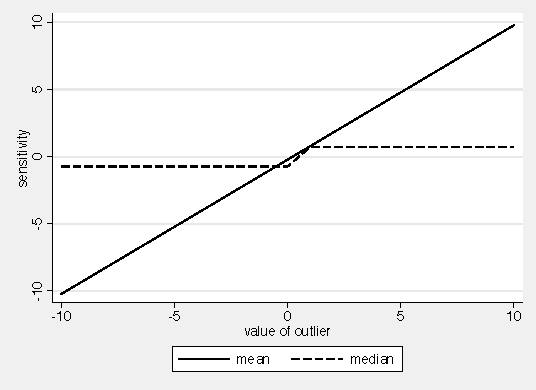
\epsfig{file=eps/2/4}
    \caption{Standardized sensitivity curves of the mean and the median for a sample of $n=20$ random $\mathcal{N}(0,1)$ numbers}
    \label{fig:theory:SClocation}
\end{figure}

\begin{figure}[h!]
    \centering
    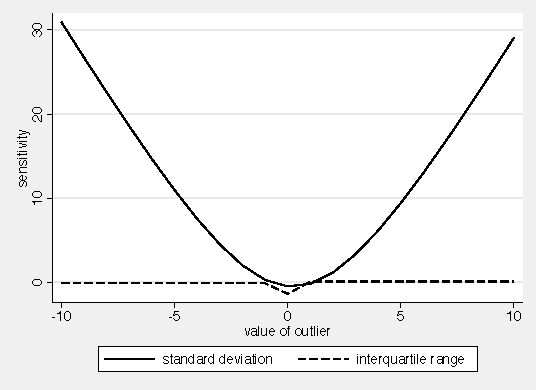
\epsfig{file=eps/2/5}
    \caption{Standardized sensitivity curves of the standard deviation and the interquartile range for a sample of $n=20$ random $\mathcal{N}(0,1)$ numbers}
    \label{fig:theory:SCscale}
\end{figure}

\index{subject}{sensitivity curve|)}

\subsubsection{The influence function}
\index{subject}{influence function|(textbf}

An intuitive way to introduce the \emph{influence function} (\stsc{IF}) of
functional $T$ at some distribution $F$ is to think of the influence function
as an asymptotic version of the \Index{sensitivity curve} of statistic $T^{(n)}=T(F^{(n)})$
when the sample size $n$ grows, so that the empirical distribution function
$F^{(n)}$ tends to the underlying population distribution function $F$ (cf.\
\citealp{hampel:1974}). More precisely, the influence function is defined as
%
\begin{align*}
    \stsc{IF}(x; T, F) 
        &= \lim_{n\rightarrow\infty} \frac{T\left(\left(1-\frac{1}{n+1}\right) F + 
            \frac{1}{n+1} \Delta_x\right) - T(F)}{\frac{1}{n+1}} \\
        &= \lim_{\varepsilon\rightarrow 0} \frac{T\left((1-\varepsilon) F + 
            \varepsilon\Delta_x\right) - T(F)}{\varepsilon}
\end{align*}
%
where $\Delta_x$ is a probability distribution with all its mass at point
$x$. That is, the influence function measures the effect on $T$ of a
perturbation of $F$ obtained by adding a small probability mass at point $x$. The expression of
$\stsc{IF}(x;T,F)$ can be found for most functionals $T$. In
chapter~\ref{chap:stats} we will provide the influence functions
of various measures of location, scale, skewness and tails heaviness.

\index{subject}{influence function|)}

\subsubsection{The gross-error sensitivity}
\index{subject}{gross-error sensitivity|(textbf}

Since $\stsc{IF}(x; T, F)$ quantifies the influence on $T$ of an infinitesimal
contamination of the distribution $F$ at point $x$, it is a \emph{local}
measure of robustness. It may be completed by a more global measure, the
\emph{gross-error sensitivity} of $T$ at distribution $F$, defined as
\[
    \gamma^*(T, F) = \sup_x \left| \stsc{IF}(x; T, F) \right|.
\]
$\gamma^*(T, F)$ evaluates to the biggest influence an outlier can have on
the functional $T$. With respect to robustness it is desirable to use an
estimator that is associated with a functional $T$ for which $\gamma^*(T, F)$ 
is finite (that is, for which the influence function is bounded).

\index{subject}{gross-error sensitivity|)}

\subsubsection{The local-shift sensitivity}
\index{subject}{local-shift sensitivity|(textbf}

The local-shift sensitivity is another tool related to the influence function;
it aims at measuring the effect of “wiggling” an observation, that is, of a
small perturbation as opposed to gross error. This is useful to asses the
effects of rounding, grouping, or other local inaccuracies.

Jumps in the \Index{influence function} (\stsc{IF}) indicate that a small
fluctuation of the value of $x$ can cause an abrupt change in the estimate.
Hence, from the perspective of robustness, we prefer a continuous \stsc{IF}
with an appropriately bounded derivative (wherever the derivative exists). 
To appreciate this kind of characteristic
of the \textit{IF}, we may determine the \emph{local-shift sensitivity}:
\[
    \lambda^*(T, F) = \sup_{x\neq y} \frac{|\stsc{IF}(y; T, F) - \stsc{IF}(x; T, F)|}
                                          {|y - x|}\ \cdot
\]

\index{subject}{local-shift sensitivity|)}

\subsubsection{The asymptotic variance of an estimator}
\index{subject}{asymptotic variance|(textbf}

The \Index{influence function} may also be used as a heuristic tool to determine the
asymptotic variance of the estimators. Indeed, under some regularity conditions
for the functional $T$, we have, under $F$,                                    
\[
    \sqrt{n}\left(T(F^{(n)}) - T(F)\right) \stackrel{d}\rightarrow \mathcal{N}\left(0, \stsc{ASV}(T, F)\right)
\]
where
\begin{equation}\label{eq:ASV}
    \stsc{ASV}(T, F) = \int_{-\infty}^\infty \stsc{IF}(x; T, F)^2 \dif F(x)
\end{equation}
(cf.\ \citealp[p. 85 and 226]{hampel:etal:1986}). Consequently, under $F$, the
interval
\[
    \left[ T(F^{(n)}) - z_{1-\alpha/2} \sqrt{\frac{\stsc{ASV}(T, F)}{n}}\ ,\  
           T(F^{(n)}) + z_{1-\alpha/2} \sqrt{\frac{\stsc{ASV}(T, F)}{n}}\right]
\]
where $z_{1-\alpha/2}$ is the quantile of order $(1-\alpha/2)$ of the ${\cal
N}(0,1)$ distribution, provides an asymptotic confidence interval for the
parameter $T(F)$, at a confidence level of $(1-\alpha)$. If the distribution
$F$, and hence the asymptotic variance $\stsc{ASV}(T, F)$, are not known, it is
still possible to obtain a confidence interval for $T(F)$ by an appropriate
\Index{resampling} method.
                                                                                \todo{\stcmd{robstat} estimates variances based
                                                                                on the “empirical” IF; this works well. Should
                                                                                maybe be explained here...}

\index{subject}{asymptotic variance|)}

\subsection{The breakdown point}
\index{subject}{breakdown point|(textbf}
\label{subsec:theory:BP}

The \Index{sensitivity curve} shows how an estimator reacts to the introduction
of one single outlier. Some estimators cannot resist even against a
single outlier. As we have seen, this is the case for the mean and the
\Index{standard deviation}. Other estimators, such as the \Index{median} and
the \Index{interquartile range}, are robust against this type of
contamination because their \Index{sensitivity curve} (\stsc{SC}) is
bounded. Possibly, however, the number of outliers in a sample is so large that
even estimators with a bounded \stsc{SC} can no longer resist their effect.
Hence, to evaluate different estimators, it is important to know what the
amount of contamination is an estimator can tolerate. The
\emph{breakdown point} is a measure for such \emph{resistance} of an estimator.
It quantifies, roughly, the smallest amount of contamination in the
sample that may cause the estimator to take on arbitrary values. Its definition
is as follows.

\subsubsection{The finite-sample breakdown point}
\index{subject}{breakdown point!finite-sample|(textbf}

The breakdown point $\epsilon^{*(n)}(T^{(n)}; \mathcal{X}^{(n)})$ of the statistic
$T^{(n)} = T^{(n)}(x_1, \dots, x_n) = T(F^{(n)})$ at the sample $\mathcal{X}^{(n)}
= \{x_1, \dots, x_n\}$ refers to the smallest proportion of observations
in $\mathcal{X}^{(n)}$ that need to be replaced to cause the value of the
statistic to be arbitrarily large or small, and hence, to make the statistic
worthless or meaningless. Note that, typically, $\epsilon^{*(n)}$ is
independent of $x_1, \dots, x_n$.

More formally, for a univariate location estimator $T^{(n)}$, which breaks down
if its absolute value becomes arbitrarily large, we may define the (finite-sample)
breakdown point as follows (see \citealp{hampel:stahel:1982};
\citealp{donoho:huber:1983}). In a given sample $\mathcal{X}^{(n)} = \{x_1,
\dots, x_n\}$, let us replace $m$ data points $x_{i_1}, \dots, x_{i_{m}}$
by arbitrary values $y_1, \dots, y_{m}$; let us call the new data set       
$\mathcal{Z}^{(n)} = \{z_1, \dots, z_n\}$. Then the \emph{(finite-sample
gross-error) breakdown point} of the estimator is
\[
    \epsilon^{*(n)}(T^{(n)}; \mathcal{X}^{(n)}) 
    = \min \left\{\left. \frac{m}{n}\right| \max_{i_i, \dots, i_{m}} \sup_{y_1, \dots, y_{m}} 
      \left|T^{(n)}(z_1, \dots, z_n)\right| =\infty \right\}.
\]

Following the same idea, we will say that a scale estimator breaks down if it
takes on a value that is arbitrarily large (scale explosion) or close to zero
(scale implosion). Furthermore, a \Index{skewness} or \Index{kurtosis}
estimator, which is bounded by $[-1, 1]$, breaks down if the absolute value of
the estimate attains the value of 1.

\begin{stexample}
If the $i$th observation among $x_1, \dots, x_n$ goes to infinity, the \Index{mean}
$\mu^{(n)}$ and the \Index{standard deviation} $\sigma^{(n)}$ go to infinity as well. This
means that the finite-sample breakdown point of these two statistics is $1/n$.
In contrast, the finite-sample breakdown point of the \Index{median} $Q_{0.5}^{(n)}$ is
$\frac{(n/2)}{n}$ if $n$ is even and $\frac{(n+1)/2}{n}$ if $n$ is odd. That is,
half the data or a bit more must be replaced to make the \Index{median} take on arbitrary
values. The finite-sample breakdown point of the \Index{interquartile range}
$\stsc{IQR}^{(n)}$ is equal to $\frac{\lfloor n/4 \rfloor + 1}{n}$, where
$\lfloor n/4 \rfloor $ denotes the integer part of $n/4$. That is, a bit more than 
one fourth of the data needs to be replaced to make the \stsc{IQR} break down.
\end{stexample}

\index{subject}{breakdown point!finite-sample|)}


\subsubsection{The asymptotic breakdown point}
\index{subject}{breakdown point!asymptotic|(textbf}

The \emph{asymptotic breakdown point} $\epsilon^*(T, F)$ of the functional
$T$ under the distribution $F$ is defined as
\[
    \epsilon^*(T, F) = \lim_{n\rightarrow\infty} \epsilon^{*(n)}(T^{(n)}; \mathcal{X}^{(n)})
\]
with the $x_i$'s sampled from $F$ (cf.\ \citealp{hampel:1971}).

\index{subject}{breakdown point!asymptotic|)}
\index{subject}{breakdown point|)}

\alert{[I would delete subsections "2.2.3 Gaussian efficiency" and "2.2.4
Aspects of interpretation". These subsections do not refer to robustness in the
presence of outliers; there are related with classical properties of
estimators, presented previously. I have modified the subsection "Summary" in
order to take into account some ideas that play an important role in the choice
of a robust estimator.]}

%\subsection{Gaussian efficiency}
%\index{subject}{Gaussian efficiency|(textbf}

%In general, if $F$ it is known, the ML-estimator for that $F$ is most efficient
%(see above). Furthermore, for $F$ equal Gaussian, the mean is the ML-estimator
%and hence most efficient. Robust estimators should not only be efficient with
%respect to Gaussian, but for a wide variety of distributions. However, Gaussian
%efficiency is also important if robust estimators are viewed as competitors of
%standard estimators. Hence it is often good to know (relative) Gaussian
%efficiency and then complement this with relative efficiencies for other
%distributions.

%\alert{[Give formal definitions etc. This is not only about Gaussian
%efficiency. For example, the mean has high variance under fat-tails
%distributions; robust estimators can have better efficiency in such cases...]}

%\index{subject}{Gaussian efficiency|)}

%\subsection{Aspects of Interpretation}

%\alert{[What about asymmetric distributions and interpretation? (e.g.
%Median vs. Mean) Need to address such aspects. The point is that robust
%estimators often estimate something that is conceptually different than the
%nonrobust counterpart (or something where robust and nonrobust counterparts
%coincide only in special situations, such as in a symmetric distribution or in
%a normal distribution).]}

\subsection{Summary}

How do we choose a good robust estimator? We are clearly interested in estimators with

\begin{enumerate}
    \item a \emph{bounded} (low \Index{gross-error sensitivity})
    and \emph{smooth} (low \Index{local-shift sensitivity}) \emph{\Index{influence function}} 

    \item and a \emph{high \Index{breakdown point}}.
\end{enumerate}

Moreover, we are looking for robust estimators that enjoy good efficiency for
a wide variety of distributions. In general, however, compromises between
robustness and efficiency must be made to achieve good overall performance, as
is shown in the following section.

Finally, we also wish to use asymptotically and Fisher consistent robust
estimators, whose rate of convergence is not smaller than the usual rate of
convergence---equal to $\sqrt{n}$---in the parametric context.


\endinput
  % Basic concepts

\chapter{Basic robust statistics}
\label{chap:stats}

Many measures of location, scale, \Index{skewness} and \Index{kurtosis} or
heaviness of the tails have been proposed and studied in the statistical
literature. The present chapter is devoted to the comparison of the
(asymptotic) \Index{Gaussian efficiency} and robustness performance of three
different classes of estimators: (i) “classic” estimators, based on (centered)
moments of the distribution $F_n$; (ii) estimators built from specific
quantiles of the distribution; (iii) estimators defined on the basis of
pairwise comparisons or combinations of the observations. In addition, we will
discuss robust test of normality and robust boxplots.

\section{Robust estimation of location}
\label{sec:stats:location}
\index{subject}{location estimators|(textbf}

There is apparent consensus in applied statistics about the fact that the
sample \Index{mean} and the sample \Index{median} are two complementary location estimators:
the mean is very efficient in case of Gaussian (i.e.\ normally distributed)
data but fragile to outliers (and problematic in case of highly asymmetric
data) while the median is very robust (and meaningful in case of asymmetry) but
rather inefficient. Both are extensively used in practice. Let us briefly
recall their respective properties and introduce two other frequently used
location estimators.

\subsection{The mean and the $\alpha$-trimmed mean}
\index{subject}{mean|(textbf}\index{subject}{$\alpha$-trimmed mean|(textbf}

The \emph{mean} corresponds to the functional $\mu = \mu(F) =
\int_{-\infty}^\infty x \dif F(x)$;                                              \todo{Comment on integrals: Why not 
                                                                                $\int x f(x)\dif x$? Maybe show somewhere that
                                                                                $\int f(x) \dif x = \int \dif F(x)$}
its empirical counterpart is $\mu_n = \mu(F_n) = \frac{1}{n} \sum_{i=1}^n x_i$.
It is well known that this location estimator is the most efficient estimator
for Gaussian data; its asymptotic variance is $\stsc{ASV}(\mu, F) =
\sigma^2$, where $\sigma^2$ denotes the variance of the distribution $F$
(taking $F = \Phi$, the standard normal distribution, we have $\stsc{ASV}(\mu,
\Phi) = 1$). Unfortunately, the mean lacks robustness. Indeed, one single
outlying observation can move this estimator towards an arbitrarily large (absolute)
value: its asymptotic breakdown point $\epsilon^*(\mu, F)$ is equal to 0.
Likewise, its influence function is unbounded, leading to an infinite
gross-error sensitivity: $\stsc{IF}(x; \mu, F) = x - \mu$ (see \citealp[p.
25]{wilcox:2005}). Figure~\ref{fig:stat:IF_loc}a shows the influence function of
$\mu$ under the standard normal distribution.                                   \todo{Why “under the standard normal distribution”?
                                                                                Isn't the influence function always the 
                                                                                same irrespective of $F$?}


\begin{figure}[h!]
    \centering
    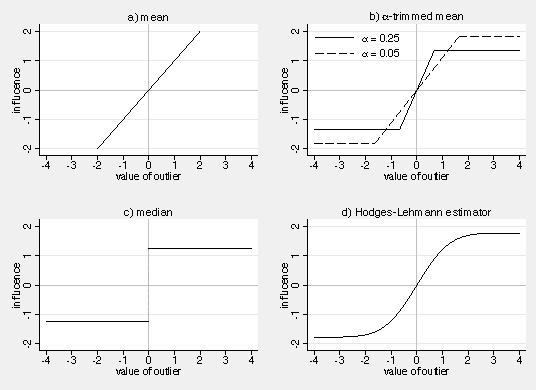
\epsfig{file=eps/3/1,width=.9\textwidth}
    \caption{Influence functions of $\mu$, $\mu^{0.25}$, $\mu^{0.05}$, $Q_{0.5}$, and $\stsc{HL}$ under the standard normal distribution}
    \label{fig:stat:IF_loc}
\end{figure}

A simple and classical way to “robustify” the sample mean consists in
discarding a certain proportion $\alpha$ ($0\leq\alpha<0.5$) of the smallest
and of the biggest observations in the sample. This leads to the
$\alpha$-\emph{trimmed mean} defined by
\[
    \mu_n^\alpha =\frac{1}{n - 2\lfloor \alpha n \rfloor}
        \sum_{i = \lfloor \alpha n \rfloor + 1}^{n - \lfloor \alpha n \rfloor} x_{(i)}
\]
where $\lfloor x \rfloor$ denotes the integer part of $x$ and $x_{(i)}$ is the
$i$th order statistic (the observation at the $i$th position in the list of
sorted observations in ascending order). Note that the sample mean $\mu_n$ is
a special case of the $\alpha$-trimmed mean $\mu_n^\alpha$ corresponding
to $\alpha = 0$. The functional associated with this location estimator is
\[
    \mu^\alpha(F) = \frac{1}{1-2\alpha} \int_{Q_\alpha}^{Q_{1-\alpha}} x \dif F(x)
\]
where $Q_\alpha = F^{-1}(\alpha)$ and $Q_{1-\alpha} = F^{-1}(1-\alpha)$ are the
$\alpha$ and $(1-\alpha)$ quantiles of distribution $F$. 

The influence function of this functional has the advantage to be bounded. If
$F$ is symmetric, then
\[
    \stsc{IF}(x; \mu^\alpha, F) = 
    \begin{cases}
        \frac{1}{1-2\alpha}\left(F^{-1}(\alpha) - \mu\right)   & \text{if $x<F^{-1}(\alpha)$} \\
        \frac{1}{1-2\alpha}(x - \mu)                           & \text{if $F^{-1}(\alpha)\leq x\leq F^{-1}(1-\alpha)$} \\
        \frac{1}{1-2\alpha}\left(F^{-1}(1-\alpha) - \mu\right) & \text{if $x>F^{-1}(1-\alpha)$}
    \end{cases}
\]
(see, e.g., \citealp{staudte:sheather:1990}). As an example, see Figure
\ref{fig:stat:IF_loc}b for the influence functions of $\mu^{0.05}$ and
$\mu^{0.25}$ under the standard Gaussian distribution $\Phi$.

Moreover, the asymptotic breakdown point of $\mu^\alpha$ is equal to
$100\alpha\%$. Clearly, hence, the proportion $\alpha$ of trimming appears as a
parameter allowing to choose the level of robustness of the trimmed mean. 
Of course, this gain in robustness goes hand in hand with a loss in efficiency.
Yet, this loss is not as large as one may fear. Using the fact that
\[
    \stsc{ASV}(\mu^\alpha, F) = \int_{-\infty}^\infty \stsc{IF}(x; \mu^\alpha, F)^2 \dif F(x)
\]
we obtain, for example,                                                         \todo{How did you compute these numbers? 
                                                                                Are there closed form solutions?}
\[
    \stsc{ASV}(\mu^{0.05}, \Phi) \approx 1.0263 \qquad
    \stsc{ASV}(\mu^{0.10}, \Phi) \approx 1.0604 \qquad
    \stsc{ASV}(\mu^{0.25}, \Phi) \approx 1.1952
\]
for the standard normal distribution. Hence, the asymptotic Gaussian relative
efficiency of $\mu^\alpha$ with respect to the mean, defined as
$\stsc{ASV}(\mu, \Phi) / \stsc{ASV}(\mu^\alpha, \Phi) = 1 /
\stsc{ASV}(\mu^\alpha, \Phi)$, reaches 97\% for $\alpha = 0.05$, 94\% for
$\alpha = 0.10$, and, despite the fact that half of the sample is discarded,
84\% for $\alpha = 0.25$.
\index{subject}{mean|)}\index{subject}{$\alpha$-trimmed mean|)}

\subsection{The median}
\index{subject}{median|(textbf}

The \emph{median}---the quantile of order 0.5---corresponds to the
functional $Q_{0.5}(F) = F^{-1}(0.5)$. Its empirical version $Q_{0.5; n}$ is
simply the sample median $F_n^{-1}(0.5)$, typically computed as
\[
    Q_{0.5;n} = 
    \begin{cases}
        x_{((n+1)/2)}                       & \text{if $n$ is odd}\\[1ex]
        \frac{x_{(n/2)} + x_{(n/2 + 1)}}{2} & \text{if $n$ is even}
    \end{cases}
\]
where $x_{(i)}$ again denotes the $i$th order statistic among $x_1, \dots,
x_n$.

The median performs better than the mean from the robustness point of view
(see, e.g., \citealp[p.\ 56 and 59]{staudte:sheather:1990}). First of all, its
influence function is given by
\[
    \stsc{IF}(x; Q_{0.5}, F) =
    \begin{cases}
        -\frac{1}{2f\left(F^{-1}(0.5)\right)} & \text{if $x < F^{-1}(0.5)$}\\[1ex]
        0                                     & \text{if $x = F^{-1}(0.5)$}\\[1ex]
        \frac{1}{2 f\left(F^{-1}(0.5)\right)} & \text{if $x > F^{-1}(0.5)$}
    \end{cases}
\]
where $f$ is the density function associated with $F$. In particular, as
displayed in Figure~\ref{fig:stat:IF_loc}c, $\stsc{IF}(x; Q_{0.5}, \Phi) =
\sign(x) \sqrt{\pi/2}$ for standard Gaussian data, since $f\left(\Phi^{-1}(0.5)\right) = \sqrt{\pi/2}$. This
influence function is bounded, leading to a bounded gross-error sensitivity, but
it has a discontinuity at $x = 0$.                                              \todo{Say why the discontinuity is a problem.}
Furthermore, the asymptotic breakdown point of
the median is equal to 50\% and is thus higher than the asymptotic breakdown
point of the $\alpha$-trimmed mean, regardless of the value of $\alpha$.

Finally, the asymptotic variance of the median is given as
\[
    \stsc{ASV}(Q_{0.5}, F) = \frac{1}{4 f\left(F^{-1}(0.5)\right)^2}
\]
Hence, relative Gaussian efficiency compared to the mean is
equal to 
\[
    \frac{\stsc{ASV}(\mu, \Phi)}{\stsc{ASV}(Q_{0.5}, \Phi)} 
    = \frac{1}{\pi/2} = \frac{2}{\pi} \approx 64\%
\]
\index{subject}{median|)}

\subsection{The Hodges-Lehmann estimator}
\index{subject}{Hodges-Lehmann estimator|(textbf}

\citet{hodges:lehmann:1963} have introduced an alternative location estimator
that has the advantage of a bounded, continuous and smooth influence
function, but also a high asymptotic Gaussian relative efficiency with respect
to the sample mean. The \emph{Hodges-Lehmann estimator} at the sample 
$\stmat{X}_n$ is defined by                                                    \todo{Can't we type
                                                                                $\stsc{HL}_n = \displaystyle\med_{i<j}\textstyle\left(\frac{x_i+x_j}{2}\right)$?
                                                                                This would seem easier to understand to me.
                                                                                Also, why only $i<j$? Why not all possible combinations (even including $i=j$)?}
\[
    \stsc{HL}_n = \med\left\{\frac{x_i+x_j}{2}; i<j \right\}
\]
It is the empirical version of the functional $\stsc{HL} = \stsc{HL}(F)$,
which is defined as the median of the distribution of $(X+Y)/2$, where $X$ and
$Y$ are i.i.d.\ random variables of distribution $F$.

For symmetric $F$, the influence function of $\stsc{HL}$ is given as
                                                                                \todo{I use $f(x)^2$ instead of 
                                                                                $f^2(x)$. I know the latter is often used in 
                                                                                stats literature, but to me the former much is
                                                                                clearer.}
\[
    \stsc{IF}(x; \stsc{HL}, F) = \frac{2 F(x-\mu) - 1}{2 \int_{-\infty}^\infty f(y)^2 \dif y}
\]
Figure~\ref{fig:stat:IF_loc}c presents the influence function for standard Gaussian
data. It illustrates that outliers have a bounded influence. Also note that the \todo{The original just said that the sensitivity
                                                                                depends on the smoothness of $F$ without saying 
                                                                                why this is relevant. I thus added some text. Please
                                                                                check, whether it is ok.}
sensitivity of the Hodges-Lehmann estimator depends on the smoothness of $F$.
Hence, the \Index{local-shift sensitivity} is small as long as the data have a  
smooth distribution function.

Because $\stsc{HL}$ combines the robust properties of the \Index{median} with the
efficiency properties of averaging, it performs well for a variety of
distributions. Based on (\ref{eq:ASV}) we obtain
\[
    \stsc{ASV}(\stsc{HL}, F) = \frac{1}{12} \left(\frac{1}{\int_{-\infty}^\infty f(y)^2 \dif y}\right)^2
\]
For example, for standard Gaussian date, $\stsc{ASV}(\stsc{HL}, \Phi) =
\pi/3 = 1.0472$. Hence, the asymptotic efficiency of the Hodges-Lehmann
estimator relative to the \Index{mean} is equal to $3/\pi \approx 95\%$ at the
normal distribution. Moreover, the Hodges-Lehmann estimator reaches a relative
efficiency with respect to the mean of at least 86\% for any symmetric
distribution (see, for example, \citealp[p. 120-121]{staudte:sheather:1990}).
Compared to the median, the Hodges-Lehmann estimator has a higher Gaussian
efficiency (95\% vs. 64\%) but a lower asymptotic breakdown point (29\% vs.
50\%).

\index{subject}{Hodges-Lehmann estimator|)}

\subsection{$M$-estimate of location}

\alert{[What about $M$-estimators???]}

\subsection{Summary}


Table \ref{tab:stat:location} summarizes the different properties of the four
location estimators. From the perspective of a good balance between high
Gaussian efficiency and a high breakdown point, the Hodges-Lehmann estimator
appears to perform particularly well.

\begin{table}[h!]
    \centering
    \caption{Characteristics of the four location estimators}
    \label{tab:stat:location}
    \begin{tabular}{lcccc}
        \toprule
        Estimator
        & Class  
        & \subtab{c}{Gaussian\\ efficiency}
        & \subtab{c}{Asymptotic\\ breakdown\\ point} 
        & \subtab{c}{Bounded\\ influence\\ function}
        \\\midrule
        mean $\mu_n$                            & moment   & 100\% &  0\%          & no
        \\\addlinespace
        $\alpha$-trimmed mean $\mu_n^{\alpha}$  & moment   & 
            \subtab{l}{$\alpha=0.05$: 97\%\\ $\alpha=0.10$: 94\%\\ $\alpha=0.25$: 84\%} 
                                                                   & $100\alpha\%$ & yes
        \\\addlinespace
        median $Q_{0.5;n}$                      & quantile & 64\%  & 50\%          & yes
        \\\addlinespace
        Hodges-Lehmann $\stsc{HL}_n$            & pairwise & 95\%  & 29\%          & yes
        \\\bottomrule
    \end{tabular}
\end{table}
\index{subject}{location estimators|)}


\section{Robust estimation of scale\label{subsec:scale}}
\index{subject}{scale estimators|(textbf}


\subsection{The standard deviation}
\index{subject}{standard deviation|(textbf}

The classic statistic to estimate the scale parameter of a distribution 
is the \emph{standard deviation} $\sigma_n$, 
corresponding to the functional 
\[
    \sigma = \sigma(F) = \sqrt{\int_{-\infty}^\infty (x-\mu)^2 \dif F(x)}
\]
At sample $\stmat{X}_n$, $\sigma_n$ is typically computed as                   \todo{I changed this to the usual 
                                                                                $1/(n-1)$ variant; if we use the 
                                                                                $1/n$ version we need to explain why.}
\[
    \sigma_n = \sigma(F_n) = \sqrt{\frac{1}{n-1} \sum_{i=1}^n (x_i-\mu_n)^2}
\]
with $\mu_n$ as defined above. The standard deviation is the most efficient
estimator of the scale parameter $\sigma$ in case of Gaussian data (note that
$\stsc{ASV}(\sigma, \Phi)=0.5$).                                               \todo{Show why $\stsc{ASV}(\sigma, \Phi)=0.5$}
However, just like the mean, the standard
deviation is very fragile to outliers. Its influence function, given as
\[
    \stsc{IF}(x; \sigma, F) = \frac{1}{2\sigma} \left(x^2 - 2\mu x + \mu^2 - \sigma^2\right)
\]
is unbounded and its asymptotic breakdown point is equal to 0\% (e.g.,
\citealp[p. 1275]{rousseeuw:croux:1993}). The influence function for standard
Gaussian data, given as $\stsc{IF}(x; \sigma, \Phi) = \frac{1}{2} (x^2 - 1)$,
is displayed in Figure~\ref{fig:stat:IF_scale}a.

\index{subject}{standard deviation|)}


\begin{figure}[h!]
    \centering
    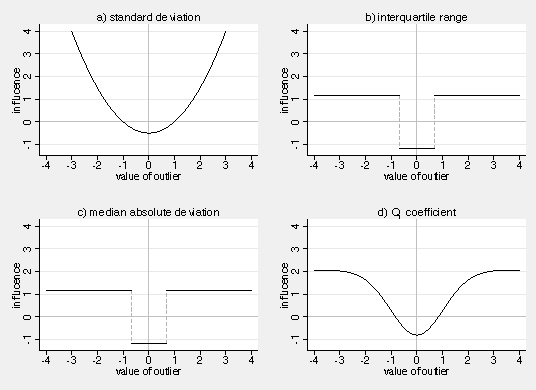
\epsfig{file=eps/3/2,width=.9\textwidth}
    \caption{Influence functions of $\sigma$, $\stsc{IQR}_c$, $\stsc{MAD}$ and $Q$ under the standard normal distribution}
    \label{fig:stat:IF_scale}
\end{figure}


\subsection{The interquartile range}
\index{subject}{interquartile range|(textbf}

A common alternative scale measure, defined on the basis of quantiles, is the
\emph{interquartile range}
\[
    \stsc{IQR}= Q_{0.75} - Q_{0.25}
\]
where $Q_{0.25}$ and $Q_{0.75}$ are the first and third quartiles of
distribution $F$. Instead of $\stsc{IQR}$ one frequently uses the
\emph{corrected interquartile range} $\stsc{IQR}_c$ defined as
\[
    \stsc{IQR}_c = d \cdot \stsc{IQR}
\]
where $d$ is a constant chosen to make the estimator $\stsc{IQR}_{c;n}$
\Index[Fisher consistency]{Fisher-consistent} for the scale parameter of the
underlying distribution. For example, for a Gaussian distribution, use $d =
1 / \left(\Phi^{-1}(0.75) - \Phi^{-1}(0.25)\right) \approx 0.7413$ to make the
corrected interquartile range a consistent estimator for the usual scale
parameter $\sigma$.

The influence function of the interquartile range is bounded, but discontinuous
(see, for example, \citealp[p. 35–36]{wilcox:2005}). It is given as
\[
    \stsc{IF}(x; \stsc{IQR}, F) =
    \begin{cases}
        \frac{1}{f\left(F^{-1}(0.25)\right)} - C & \text{if $x < F^{-1}(0.25)$}\\[1ex]
        -C                                       & \text{if $F^{-1}(0.25) \leq x \leq F^{-1}(0.75)$}\\[1ex]
        \frac{1}{f\left(F^{-1}(0.75)\right)} - C & \text{if $x > F^{-1}(0.75)$}
    \end{cases}
\]
where 
\[
    C = \frac{1}{4} \left[\frac{1}{f\left(F^{-1}(0.25)\right)} + \frac{1}{f\left(F^{-1}(0.75)\right)}\right]
\]

Note that $\stsc{IF}(x; \stsc{IQR}_c, F) = d \cdot \stsc{IF}(x;
\stsc{IQR}, F)$. Figure~\ref{fig:stat:IF_scale}b displays the influence
function of $\stsc{IQR}_c$ for standard Gaussian data. Like the two quartiles
$Q_{0.25}$ and $Q_{0.75}$, $\stsc{IQR}$ and $\stsc{IQR}_c$ have an
asymptotic breakdown point equal to 25\%. This gain in robustness with respect
to the standard deviation is accompanied by a high loss in Gaussian
efficiency. Specifically, $\stsc{ASV}(\stsc{IQR}_c, \Phi) = 1.3605$ so that      \todo{Give details about $\stsc{ASV}(\stsc{IQR}_c, \Phi)$. How is it computed?}
the asymptotic Gaussian efficiency of the corrected interquartile range with
respect to the standard deviation is equal to $\stsc{ASV}(\sigma, \Phi) /
\stsc{ASV}(\stsc{IQR}_c, \Phi) = 0.5/1.3605 \approx 37\%$.

\index{subject}{interquartile range|)}

\subsection{The median absolute deviation}
\index{subject}{median absolute deviation|(textbf}

Another robust alternative is the \emph{median absolute deviation}, whose
empirical version is defined as
\[
    \stsc{MAD}_n = d \cdot \med_i\left|x_i-\med_j x_j\right|
\]
That is, the median absolute deviation is equal to the (rescaled) median of the
absolute deviations from the median of the variable of interest. For Gaussian
distributions, we need to set $d = 2 / \left(\Phi^{-1}(0.75) -
\Phi^{-1}(0.25)\right) \approx 1.4826$ to make $\stsc{MAD}_n$
Fisher-consistent for the scale parameter $\sigma$.

The functional corresponding to $\stsc{MAD}_n$ is 
\[
    \stsc{MAD} = \stsc{MAD}(F) = d \cdot G_{F}^{-1}(0.5)
\]
where $G_{F}$ is the distribution function of $|X-Q_{0.5}(F)| = |X-F^{-1}(0.5)|$ 
with $X$ as a random variable of distribution $F$. In other
words, $\stsc{MAD}$ is equal to $d$ times the median of the distribution
associated with $|X-Q_{0.5}(F)|$, the magnitude of the difference between $X$
and its median.

The median absolute deviation may appear more attractive than the
interquartile range for certain purposes. It has the same asymptotic
Gaussian efficiency as the corrected interquartile range, but performs better
in terms of robustness (e.g., \citealp[p. 1273–1274]{rousseeuw:croux:1993}):
Its asymptotic breakdown point is as high as 50\%. The influence function 
of $\stsc{MAD}$ is given as $d \cdot \stsc{IF}(x; G_{F}^{-1}(0.5), F)$ with
\[
    \stsc{IF}(x; G_{F}^{-1}(0.5), F)
    = \frac{\sign\left(|x-F^{-1}(0.5)| - G_{F}^{-1}(0.5)\right) - C \cdot \sign\left(x-F^{-1}(0.5)\right)}
    {2 \left[f\left(F^{-1}(0.5) + G_{F}^{-1}(0.5)\right) + f\left(F^{-1}(0.5) - G_{F}^{-1}(0.5)\right)\right]}
\]
where
\[
    C = \frac{f\left(F^{-1}(0.5) + G_{F}^{-1}(0.5)\right) - f\left(F^{-1}(0.5) - G_{F}^{-1}(0.5)\right)}
    {f\left(F^{-1}(0.5)\right)}
\]
(see, e.g., \citealp{wilcox:2005}). In particular, under the standard Gaussian
distribution (with $F=\Phi$ and $f=\phi$), we have                              \todo{Is it only for Gaussian data 
                                                                                that the IF for IQR and MAD is the same,
                                                                                or is this true for any symmetric 
                                                                                distribution?}
\[
    \stsc{IF}(x; \stsc{MAD}, \Phi) 
    = 1.4826 \cdot\frac{\sign\left(|x| - \Phi^{-1}(0.75)\right)}
                       {4\,\phi\left(\Phi^{-1}(0.75)\right)}
\]
which is displayed in Figure \ref{fig:stat:IF_scale}c.                          \todo{In Rousseeuw/Croux the IF of MAD is closer to that one of Q; check that...}


Despite its good robustness properties, $\stsc{MAD}$ is primarily useful for
\emph{symmetric} distributions. In fact, the $\stsc{MAD}$ corresponds to
finding the symmetric interval around the median that contains 50\% of the data
(50\% of the probability mass), which does not appear to be a very sensible
approach for asymmetric distributions. The interquartile range does not have
this restriction, as the quartiles need not be equally far away from the median.

\index{subject}{median absolute deviation|)}


\subsection{The $Q_n$ coefficient}

Finally, a very interesting but relatively unknown scale estimator is the
$Q_n$ statistic introduced by \citet{rousseeuw:croux:1993}:
\[
    Q_n =   d\cdot \{|x_i-x_j|; i<j\}_{(k)}
\]
where $d$ is a constant factor allowing $Q_n$ to be a Fisher-consistent
estimator for the scale parameter of the underlying distribution $F$ and $k =
\binom{h}{2} \approx \binom{n}{2}/4$, with $h = \lfloor n/2\rfloor + 1$ ($h$ is
roughly half the number of observations). In other words, if we omit the
constant $d$, the statistic $Q_n$ corresponds approximately to the 0.25
quantile of the $\binom{n}{2}$ distances $|x_i-x_j|$, $i<j$. Fisher-consistency for the 
scale parameter $\sigma$ at Gaussian distributions can be achieved by setting
$d = 1/\left(\sqrt{2}\Phi^{-1}(5/8)\right) \approx 2.2191$.                     \todo{In Rousseeuw/Croux the value is 2.2219,
                                                                                 which seems to be an error.}

The functional counterpart of $Q_n$ is 
\[
    Q = Q(F) = d\cdot H_{F}^{-1}(0.25)
\]
where $H_{F}$ is the distribution function of $|X-Y|$ with $X$ and $Y$ being two
independent random variables of distribution $F$. Note that $Q(F_n)$ is not
exactly the same as $Q_n$, where we take an order statistic among $\binom{n}{2}$
elements instead of $n^2$ elements, but asymptotically this makes no difference.

The scale estimator $Q_n$ has globally better properties than the previous
scale estimators we have presented. Like the $\stsc{MAD}$, it has an asymptotic
breakdown point equal to 50\%. Yet, unlike the $\stsc{MAD}$, $Q_n$ is not
slanted towards symmetric distributions. Moreover, its influence function is
not only bounded, but also smooth:                                              \todo{I use numerical integration to obtain 
                                                                                the value of the denominator (used for the 
                                                                                graph and for the computation of the efficiency).
                                                                                Is there also a closed-form solution?}
\[
    \stsc{IF}(x; Q, F) = d\cdot \frac{0.25 - F(x+d^{-1}) + F(x-d^{-1})}{\int_{-\infty}^\infty f(y+d^{-1}) \dif F(y)}
\]
Figure~\ref{fig:stat:IF_scale}d displays the influence function of $Q_n$ for 
standard Gaussian data.                                                         

Finally, $Q_n$ is asymptotically more efficient than the median absolute
deviation under Gaussian distributions. In particular, numerical integration of
$\int_{-\infty}^\infty \stsc{IF}(x;Q,\Phi)^2 \dif \Phi(x)$ yields
$\stsc{ASV}(Q,\Phi) \approx .6089$, corresponding to an asymptotic Gaussian        \todo{I get 0.6089, not 0.6077.}
relative efficiency with respect to the standard deviation of
$\stsc{ASV}(\sigma, \Phi) / \stsc{ASV}(Q, \Phi) \approx 0.5/.6089 \approx 82\%$,
which is surprisingly high.

\todo{The following output shows my computations. Results should     be precise (e.g., they do not change if I increase the number of              integration points to 100000). This is just for you. It will be removed       later on.}
\begin{stlog}
. use Star.dta, clear
{\smallskip}
. regress log_intensity log_temperature
{\smallskip}
      Source {\VBAR}       SS           df       MS      Number of obs   =        47
\HLI{13}{\PLUS}\HLI{34}   F(1, 45)        =      2.08
       Model {\VBAR}  .664593334         1  .664593334   Prob > F        =    0.1557
    Residual {\VBAR}  14.3463934        45  .318808743   R-squared       =    0.0443
\HLI{13}{\PLUS}\HLI{34}   Adj R-squared   =    0.0230
       Total {\VBAR}  15.0109868        46  .326325799   Root MSE        =    .56463
{\smallskip}
\HLI{14}{\TOPT}\HLI{64}
log_intensity {\VBAR}      Coef.   Std. Err.      t    P>|t|     [95\% Conf. Interval]
\HLI{14}{\PLUS}\HLI{64}
log_tempera{\tytilde}e {\VBAR}  -.4133041   .2862575    -1.44   0.156    -.9898562     .163248
        _cons {\VBAR}   6.793468   1.236516     5.49   0.000     4.302998    9.283939
\HLI{14}{\BOTT}\HLI{64}
{\smallskip}

\end{stlog}

\subsection{Summary}

To conclude, Table \ref{tab:stat:scale} summarizes the different properties of the
presented estimators of scale. As is evident, the $Q_n$ coefficient has superior
properties in terms of robustness and efficiency compared to the other robust 
estimators.

\begin{table}[h!]
    \centering
    \caption{Characteristics of the four scale estimators}
    \label{tab:stat:scale}
    \begin{tabular}{lcccc}
        \toprule
        Estimator
        & Class  
        & \subtab{c}{Gaussian\\ efficiency}
        & \subtab{c}{Asymptotic\\ breakdown\\ point} 
        & \subtab{c}{Bounded\\ influence\\ function}
        \\\midrule
        standard deviation $\sigma_n$              & moment   & 100\% &  0\% & no
        \\\addlinespace
        interquartile range $\stsc{IQR}_n$       & quantile & 37\%  & 25\% & yes
        \\\addlinespace
        median absolute deviation $\stsc{MAD}_n$ & quantile & 37\%  & 50\% & yes
        \\\addlinespace
        $Q_n$ coefficient                 & pairwise & 82\%  & 50\% & yes
        \\\bottomrule
    \end{tabular}
\end{table}

\index{subject}{scale estimators|)}


\section{Robust estimation of skewness}
\label{subsec:skewness}
\index{subject}{skewness estimators|(textbf}

\subsection{The Fisher coefficient}
\index{subject}{Fisher coefficient|(textbf}

As far as skewness is concerned, the most classic estimator is the \emph{Fisher
coefficient}. Given sample $\stmat{X}_n$ the Fisher coefficient is defined as
\[
    \gamma_{1; n} = \frac{1}{n} \sum_{i=1}^n\left(\frac{x_i - \mu_n}{\sigma_n}\right)^{3}
\]
with $\mu_n$ and $\sigma_n$ as the sample \Index{mean} and the 
\Index{standard deviation}. This estimator is associated with the functional
\[
    \gamma_1 = \gamma_1(F) = \mu_{3}(F)/\sigma(F)^3
    \qquad\text{where}\quad
    \mu_{3}(F) = \int_{-\infty}^\infty \left(x-\mu(F)\right)^3 \dif F(x)
\]
which is equal to zero at symmetric $F$. 

Since the Fisher coefficient relies on the \Index{mean} and the \Index{standard
deviation}, it is not surprising that its resistance to outliers is poor. More
precisely, its asymptotic \Index{breakdown point} is equal to 0\% and its
\Index{influence function} is unbounded (see, for example,
\citealp{groeneveld:1991}). For a \emph{symmetric} distribution $F$, assuming $\mu(F)
= 0$ and $\sigma(F) = 1$ without loss of generality, the influence function of  \todo{What exactly does this mean? Is the IF always 
                                                                                like that irrespective of $\mu$ and $\sigma$ or 
                                                                                is it different, but does not change shape? (In this case: What would be 
                                                                                the IF for $\mu\neq 0$ and $\sigma\neq 1$?)}
the Fisher coefficient is given as
\[
    \stsc{IF}(x; \gamma_1, F) = x^{3} - 3x
\]
See Figure~\ref{fig:stat:IF_skew}a for a graphical display. The influence
function for an \emph{asymmetric} distribution is more complex. However,
although no longer being an odd function of $x$, it has a quite similar form to
that found for symmetric $F$. Also note, for comparisons with other skewness
estimators, that $\stsc{ASV}(\gamma_1, \Phi) = 6$.                            \todo{How is this found?}

\index{subject}{Fisher coefficient|)}


\begin{figure}[h!]
    \centering
    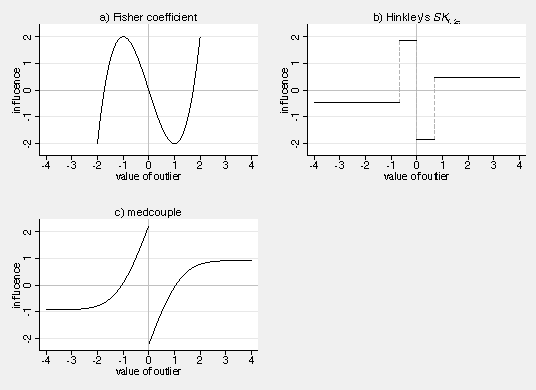
\epsfig{file=eps/3/4,width=.9\textwidth}
    \caption{Influence functions of $\gamma_1$, $\stsc{SK}_{0.25}$ and $\stsc{MC}$ under the standard normal distribution}
    \label{fig:stat:IF_skew}
\end{figure}

\subsection{Yule and Kendall, and Hinkley skewness measures}
\index{subject}{Yule and Kendall skewness|(textbf}
\index{subject}{Hinkley skewness|(textbf}

Alternative estimators of skewness, such as $(\mu_n-\text{mode}_n)/\sigma_n$ 
and $(\mu_n-Q_{0.5;n})/\sigma_n$ as proposed by Karl Pearson,
are just as fragile with respect to outliers as the standard
skewness estimator. 

Fortunately, robust alternatives based on quantiles are
available. For example, Yule and Kendall have proposed the skewness measure     \todo{Do you have a citation for this?}
\[
    \stsc{SK}_{\stsc{YK}}
    = \frac{(Q_{0.75} - Q_{0.5}) - (Q_{0.5}-Q_{0.25})}{Q_{0.75} - Q_{0.25}}
    = \frac{Q_{0.25} + Q_{0.75} - 2Q_{0.5}}{Q_{0.75} - Q_{0.25}}
\]
where $Q_{0.25}$, $Q_{0.5}$, and $Q_{0.75}$ are the three quartiles.

\citet{hinkley:1975} generalized this formula to other quantiles:
\[
    \stsc{SK}_p 
    = \frac{(Q_{1-p} - Q_{0.5}) - (Q_{0.5} - Q_p)}{Q_{1-p} - Q_p}
    = \frac{Q_p + Q_{1-p} - 2Q_{0.5}}{Q_{1-p} - Q_p},
\]
where $Q_p$ and $Q_{1-p}$ are the quantiles of order $p$ and $1-p$ (with
$0<p<0.5$). Hinkley's measure $\stsc{SK}_p$ is equal to zero for symmetric
distributions, is positive for right tailed (left skewed) and negative for left
tailed (right skewed) distributions. It has a much smaller asymptotic variance
under the standard normal distribution than $\gamma_1$. For instance,
$\stsc{ASV}(\stsc{SK}_{0.25}, \Phi) = 1.8421$.                                  \todo{How is the ASV derived? Plus: what is the expected value of $Q_{0.25}$ for Gaussian data?}
The asymptotic breakdown point of $\stsc{SK}_p$ is equal to $100p\%$ (in
particular, the Yule and Kendall skewness estimator, corresponding to $p=0.25$,
has an asymptotic breakdown point equal to 25\%).

For a \emph{symmetric} distribution $F$ with density $f$ and, without loss of
generality, $\mu(F) = F^{-1}(0.5) = 0$ and $\sigma(F) = 1$, the influence
function of $\stsc{SK}_p$ is
\[
    \stsc{IF}(x; \stsc{SK}_p, F) =
    \begin{cases}
        \frac{-1 / f(0)}{F^{-1}(1-p) - F^{-1}(p)}                            & \text{if $0\leq x < F^{-1}(1-p)$} \\[1ex]
        \frac{1/f\left(F^{-1}(1-p)\right) - 1/f(0)}{F^{-1}(1-p) - F^{-1}(p)} & \text{if $F^{-1}(1-p)\leq x$}
    \end{cases}
\]
for $x \geq 0$ and $\stsc{IF}(x; \stsc{SK}_p, F) = -\stsc{IF}(-x;
\stsc{SK}_p, F)$ for $x<0$. The influence function for standard Gaussian data
is displayed in Figure~\ref{fig:stat:IF_skew}b. In case of an
\emph{asymmetric} distribution the influence function is much more complex
and is no longer an odd function of $x$ (see \citealp[p.~101]{groeneveld:1991}).

\index{subject}{Yule and Kendall skewness|)}
\index{subject}{Hinkley skewness|)}

\subsection{The medcouple}
\index{subject}{medcouple|(textbf}

As usual when working with quantiles, the influence function of $\stsc{SK}_p$
is not smooth. To tackle this problem, \citet{brys:etal:2004a} propose to
replace the quantiles $Q_p$ and $Q_{1-p}$ in $\stsc{SK}_p$ by actual data
points and introduce a new skewness measure called \emph{medcouple}. 
Let $x_{(1)}\leq x_{(2)}\leq\dots\leq x_{(n)}$ be the $n$ order
statistics associated to the sample $\stmat{X}_n$ and $Q_{0.5;n}$ be 
the sample median. The medcouple is then defined as
\[
    \stsc{MC}_n =\med_{x_{(i)} \leq Q_{0.5;n} \leq x_{(j)}} 
    h \left(x_{(i)}, x_{(j)}\right)
\]
where, for all $x_{(i)} \neq x_{(j)}$, the kernel function $h$ is given as
\[
    h\left(x_{(i)}, x_{(j)}\right) = 
    \frac{\left(x_{(j)} - Q_{0.5;n}\right) - \left(Q_{0.5;n} - x_{(i)}\right)}{x_{(j)}-x_{(i)}}
\]
For the special case $x_{(i)}=x_{(j)}=Q_{0.5;n}$, the kernel is defined as
follows: let $m_1 < \dots < m_{k}$ denote the indices of the order statistics
that are tied to the median $Q_{0.5;n}$ (that is $x_{(m_{l})}  =Q_{0.5;n}$ for  \todo{What about other ties, i.e. $x_{(i)}=x_{(j)}\neq 
                                                                                Q_{0.5;n}$? $h()$ is not defined for these cases because
                                                                                the denominator is 0. Should $h()$ be defined as 0 in this 
                                                                                case?}
all $l=1,\dots,k$). Then,
\[
    h \left(x_{(m_i)}, x_{(m_j)}\right) =
    \begin{cases}
        -1  & \text{if $i+j<k+1$}\\
        0   & \text{if $i+j=k+1$}\\
        1   & \text{if $i+j>k+1$}\\
    \end{cases}
\]
Due to the denominator it is clear that $h\left(x_{(i)}, x_{(j)}\right)$, 
and hence $\stsc{MC}_n$, will always lie between $-1$ and $1$ (similar to
$\stsc{SK}_p$).

The functional form of the medcouple is simply defined at any continuous
distribution $F$ as 
\[
    \stsc{MC} = \stsc{MC}(F) = \med_{X \leq Q_{0.5} \leq Y} h(X,Y)
\]
where $Q_{0.5}=F^{-1}(0.5)$ is the median of $F$ and $X$ and $Y$ are i.i.d.
random variables of distribution $F$. The kernel $h$ is the same as above with
the finite-sample median $Q_{0.5;n}$ replaced by $Q_{0.5}$. This functional
$\stsc{MC}$ is equal to zero in case of a symmetric distribution $F$. It is
positive for right tailed (left skewed) and negative left tailed (right skewed)
distributions.

The asymptotic breakdown point of the medcouple is equal to 25\%, which is the
same as for the quartile skewness $\stsc{SK}_{0.25}=\stsc{SK}_\stsc{YK}$. 
The advantage of $\stsc{MC}$, however, lies in the fact that its
influence function resembles a smoothed version of the influence function
of $\stsc{SK}_p$ ($0<p<0.5$). In particular, for standard Gaussian $F$, the   \todo{Why $\stsc{SK}_p$? Why not $\stsc{SK}_{0.25}$?} 
influence function is given as
\[
    \stsc{IF}(x; \stsc{MC}, \Phi) = \pi \left(2\Phi(x) - 1 - \frac{\sign(x)}{\sqrt{2}}\right)
\]
(see Figure~\ref{fig:stat:IF_skew}c). This leads to an asymptotic variance for
Gaussian data of                                                                \todo{Is 1.25 an exact result? How do you compute that? Plus: what is the expected value of medcouple for Gaussian data?}
\[
    \stsc{ASV}(\stsc{MC}, \Phi) = \int_{-\infty}^{\infty} \stsc{IF}(x;\stsc{MC},\Phi)^2 \dif \Phi(x) = 1.25
\]


\index{subject}{medcouple|)}

\subsection{Summary}

Table \ref{tab:stat:skewness} provides an overview of the
properties of the discussed skewness estimators. As can be seen, both proposed
robust estimators are more robust and, at the same time, more efficient than 
the standard skewness coefficient.                                              \todo{How to compute efficiency? Need to rescale...}

\begin{table}[h!]
    \centering
    \caption{Characteristics of the three skewness estimators}
    \label{tab:stat:skewness}
    \begin{tabular}{lcccc}
        \toprule
        Estimator
        & Class  
        & \subtab{c}{Gaussian\\ efficiency\textsuperscript{\textit{a}}}
        & \subtab{c}{Asymptotic\\ breakdown\\ point} 
        & \subtab{c}{Bounded\\ influence\\ function}
        \\\midrule
        Fisher coefficient $\gamma_{1;n}$     & moment   & 100\%        &  0\% & no
        \\\addlinespace
        Hinkley's $\stsc{SK}_{0.25;n}$      & quantile & \alert{???} & 25\% & yes
        \\\addlinespace
        medcouple $\stsc{MC}_n$             & pairwise & \alert{???} & 25\% & yes
        \\\bottomrule
        \multicolumn{5}{l}{\footnotesize\textsuperscript{\textit{a}} relative to the 
        efficiency of the Fisher coefficient}
    \end{tabular}
\end{table}

\index{subject}{skewness estimators|)}

\section{Robust estimation of the tails heaviness}
\label{subsec:kurtosis}
\index{subject}{kurtosis estimators|(textbf}

\subsection{The classical kurtosis coefficient}

The classical \emph{kurtosis coefficient} is defined by the functional
\[
    \gamma_2 = \gamma_2(F) = \mu_{4}(F)/\sigma(F)^{4}
\]
with
\[
    \mu_{4}(F) = \int_{-\infty}^\infty \left(x-\mu(F)\right)^{4} \dif F(x)
\]
Given a sample $\stmat{X}_n$, $\gamma_{2;n}$ is computed as
\[
    \gamma_{2;n} = \frac{1}{n} \sum_{i=1}^n \left(\frac{x_i-\mu_n}{\sigma_n}\right)^{4}
\]
with $\mu_n$ and $\sigma_n$ as the sample \Index{mean} and the \Index{standard
deviation}. 

The kurtosis coefficient is often considered as a measure of the
tail heaviness of a distribution relative to that of the normal distribution.
In particular, $\gamma_2$ is equal to three in case of distributions with a
tails heaviness similar to the normal distribution, is larger than three for
leptokurtic distributions (i.e., distributions with heavier tails than the
normal distribution) and is smaller than three for platokurtic distributions
(i.e., distributions with lighter tails than the normal distribution).
However, since the coefficient also measures the peakedness of a
distribution, there is no agreement on what the kurtosis really estimates. Another
disadvantage of the kurtosis is that its interpretation, and consequently its
use, is restricted to symmetric distributions (due of its intrinsic
comparison with the symmetric normal distribution). Moreover, as usual for
estimators relying on the mean and the standard deviation, the kurtosis
coefficient is very sensitive to outliers in the data. This is reflected in
the asymptotic breakdown point being equal to zero. The influence function is unbounded 
and is given as
\[
    \stsc{IF}(x; \gamma_2,F) = (z^2-\gamma_2)^2 - \gamma_2(\gamma_2-1) - 4\gamma_1 z,
\]
where $z = \left(x-\mu(F)\right)/\sigma(F)$, $\gamma_1 = \mu_{3}(F)/\sigma(F)^{3}$ and
$\gamma_2 = \mu_{4}(F)/\sigma(F)^{4}$ (see \citealp{ruppert:1987}).
See Figure~\ref{fig:stat:IF_tail}a for a graphical display of the influence function for 
standard Gaussian $F$, which is given as $\stsc{IF}(x; \gamma_2, \Phi) = (x^2-3)^2-6$.
The form of the influence function indicates that contamination
at the center has far less influence than that in the extreme tails. This
suggests that $\gamma_2$ is primarily a measure of tail behavior, and only
to a lesser extent of peakedness. The asymptotic variance of $\gamma_2$ for Gaussian 
data is given as $\stsc{ASV}(\gamma_2, \Phi) = 24$.                           \todo{Closed form solution?}



\begin{figure}[h!]
    \centering
    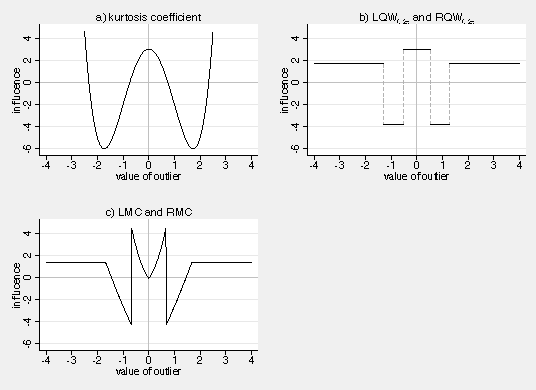
\epsfig{file=eps/3/5,width=.9\textwidth}
    \caption{Influence functions of $\gamma_2$, $\stsc{LQW}_{0.25}$ and $\stsc{RQW}_{0.25}$, $\stsc{LMC}$ and $\stsc{RMC}$ under the standard normal distribution}
    \label{fig:stat:IF_tail}
\end{figure}

\subsection{The quantile and medcouple tail weight measures}

To overcome the problems of the kurtosis coefficient, \citet{brys:etal:2006}
have proposed two measures of \emph{left} and \emph{right} tail weight for
univariate continuous distributions. As discussed below, these measures have
the advantage that they can be applied to symmetric as well as asymmetric
distributions that do not need to have finite moments. Moreover, their
interpretation is unambiguous and they are robust against outlying values.

More precisely, \citet{brys:etal:2006} defined \emph{left} and \emph{right}
tail measures as measures of skewness that are applied to the half of the
probability mass lying on the left side or on the right side of the median
$Q_{0.5}$ of the distribution $F$, respectively. As candidate measures of skewness 
they use both, $\stsc{SK}_p$ ($0<p<0.5$) and $\stsc{MC}$ (see above).

Recall that $\stsc{SK}_p$ is a measure of skewness of the distribution $F$
around $Q_{0.5}$, involving the quantiles $Q_p$ and $Q_{1-p}$ of orders $p$
and $(1-p)$ of $F$. Applying $-\stsc{SK}_{p/2}$ to the left half of the
distribution $F$ (i.e., to $x<Q_{0.5}$) leads to the \emph{Left Quantile
Weight} $\stsc{LQW}_p = \stsc{LQW}_p(F)$, which corresponds to (the
opposite of) a measure of skewness of the left half of $F$ around the first
quartile $Q_{0.25}$ involving the quantiles $Q_{p/2}$ and $Q_{0.5-p/2}$:
\[
    \stsc{LQW}_p 
    = -\frac{(Q_{0.5-p/2} - Q_{0.25}) - (Q_{0.25} - Q_{p/2})}{Q_{0.5-p/2}-Q_{p/2}}
    = -\frac{Q_{p/2}  +Q_{0.5-p/2} - 2 Q_{0.25}}{Q_{0.5-p/2} - Q_{p/2}}.
\]
Similarly, applying $\stsc{SK}_{p/2}$ to the right half of the distribution
$F$ (i.e., to $x>Q_{0.5}$) provides the \emph{Right Quantile Weight}
$\stsc{RQW}_p = \stsc{RQW}_p(F)$ which corresponds to a measure of
skewness of the right half of $F$ around the third quartile $Q_{0.75}$
involving the quantiles $Q_{0.5+p/2}$ and $Q_{1-p/2}$:
\[
    \stsc{RQW}_p
    = \frac{(Q_{1-p/2} - Q_{0.75}) - (Q_{0.75} - Q_{0.5+p/2})}{Q_{1-p/2} - Q_{0.5+p/2}}
    = \frac{Q_{0.5+p/2} + Q_{1-p/2} - 2 Q_{0.75}}{Q_{1-p/2} - Q_{0.5+p/2}}.
\]
With $p = 1/4 = 0.25$, we obtain
%
\begin{align*}
    \stsc{LQW}_{0.25} & = -\frac{Q_{0.125} + Q_{0.375} - 2 Q_{0.25}}{Q_{0.375} - Q_{0.125}}\\[1ex]
    \stsc{RQW}_{0.25} & =  \frac{Q_{0.625} + Q_{0.875} - 2 Q_{0.75}}{Q_{0.875} - Q_{0.625}}
\end{align*}
%
Note that the sample versions $\stsc{LQW}_{p;n}$ and $\stsc{RQW}_{p;n}$
are easily found by using the quantiles of $F_n$, the empirical distribution
function of $\stmat{X}_n$.

As with $\stsc{LQW}$ and $\stsc{RQW}$, we can also apply the $\stsc{MC}$ to
each side of the distribution, leading to the \emph{Left Medcouple}
($\stsc{LMC}$) and to the \emph{Right Medcouple} ($\stsc{RMC}$), defined
as
%
\begin{align*}
    \stsc{LMC} &=\stsc{LMC}(F) = -\stsc{MC}(x<Q_{0.5})\\[1ex]
    \stsc{RMC} &=\stsc{RMC}(F) = \stsc{MC}(x>Q_{0.5})
\end{align*}
%
By using $\stsc{MC}_n$, the finite-sample version of $\stsc{MC}$, we
obtain the finite-sample versions $\stsc{LMC}_n$ and $\stsc{RMC}_n$.

Since both the quantile and the medcouple tail weight measures only depend on
quantiles, they are given for any distribution, even for distributions without
finite moments. Note that $\stsc{LQW}$ and $\stsc{RQW}$ require to fix the
parameter $p$ in advance (depending on the degree of robustness one wants to
attain), whereas $\stsc{LMC}$ and $\stsc{RMC}$ do not require any
additional parameter to be set.

Some general properties of the tail weight measures are as follows. 
Let $X$ be a random variable with continuous distribution $F_X$. Furthermore, 
let $\stsc{W}$ stand for any of the defined tail weight measures; 
let $\stsc{LW}$ stand for left tailed measures and $\stsc{RW}$ 
for the right tailed measures. Then:
\begin{itemize}
    \item Like the skewness measures $\stsc{SK}_p$ and $\stsc{MC}$,
    $\stsc{W}$ is location and scale invariant. That is, $\stsc{W}(F_{aX+b}) = \stsc{W}(F_X)$.

    \item $\stsc{LW}(F_{-X}) = \stsc{RW}(F_X)$.

    \item If $F$ is symmetric, then $\stsc{LW}(F) = \stsc{RW}(F)$.

    \item $\stsc{W} \in[-1,1]$.
\end{itemize}

The medcouple tail weight measures can resist up to 12.5\% outliers in the
data. In a similar way, it can be shown that the left and right quantile tail
weight measures $\stsc{LQW}_p$ and $\stsc{RQW}_p$ have an asymptotic
breakdown point equal to $(100p/2)\%$; in particular, $\stsc{LQW}_{0.25}$
and $\stsc{RQW}_{0.25}$ have the same asymptotic breakdown point as
$\stsc{LMC}$ and $\stsc{RMC}$, and $\stsc{LQW}_{0.125}$ and
$\stsc{RQW}_{0.125}$ have an asymptotic breakdown point of 6.25\%.

Moreover, the influence functions of $\stsc{LMC}$ and $\stsc{RMC}$ are
smooth versions of the influence functions of $\stsc{LQW}_{0.25}$ and
$\stsc{RQW}_{0.25}$, as shown in Figure~\ref{fig:stat:IF_tail}b and c for
standard Gaussian $F$.\footnote{Figure~\ref{fig:stat:IF_tail} shows only the
left part (defined on ${\mathbb{R}}^{-}$) of the influence functions of
$\stsc{LMC}$ and $\stsc{LQW}_{0.25}$, and the right part (defined on
${\mathbb{R}}^{+}$) of the influence functions of $\stsc{RMC}$ and
$\stsc{RQW}_{0.25}$.} All these influence functions are bounded. More
precisely, if $F$ is a continuous distribution with density $f$ and if we
denote, as usual, the quantile of order $p$ of $F$ by $Q_p=F^{-1}(p)$, we have
\[
    \stsc{IF}(x; \stsc{LQW}_p, F) 
         = 2\, \frac{\begin{array}{@{}l@{}}
                    \left(\stsc{IF}(x; Q_{0.25}, F) - \stsc{IF}(x; Q_{0.5-p/2}, F)\right)
                                       \left(q_{0.25} - Q_{p/2}\right)\\
                    \qquad - \left(\stsc{IF}(x; Q_{p/2}, F) - \stsc{IF}(x;Q_{0.25},F)\right) 
                                       \left(Q_{0.5-p/2} - Q_{0.25}\right)
                    \end{array}}
            {\left(Q_{0.5-p/2} - Q_{p/2}\right)^2}
\]
and
\[
    \stsc{IF}(x; \stsc{RQW}_p, F) 
         = 2\, \frac{\begin{array}{@{}l@{}}
                    \left(\stsc{IF}(x; Q_{0.5+p/2}, F) - \stsc{IF}(x; Q_{0.75}, F)\right)
                                       \left(q_{1-p/2} - Q_{0.75}\right)\\
                    \qquad - \left(\stsc{IF}(x; Q_{0.75}, F) - \stsc{IF}(x;Q_{1-p/2},F)\right) 
                                       \left(Q_{0.75} - Q_{0.5+p/2}\right)
                    \end{array}}
            {\left(Q_{1-p/2} - Q_{0.5+p/2}\right)^2}
\]
with 
\[
    \stsc{IF}(x; Q_p, F) = \frac{p - \I[x<Q_p]}{f(Q_p)}
\]
The expression of the influence functions of $\stsc{LMC}$ and $\stsc{RMC}$
is more complex and can be found in \citet[p.~740--741]{brys:etal:2006}.        \todo{(maybe have a look and then 
                                                                                check computation of graph; it seems IF
                                                                                has a discontinuity; need to use shortdash)}

Finally, the asymptotic variances of the left and right tail weight measures    
under Gaussian distributions are much smaller than the variance of the classical
kurtosis coefficient $\gamma_2$. In particular:                                 \todo{How are these numbers computed? Furthermore,
                                                                                is it a fair comparison. That is, are L/RQW and L/RMC
                                                                                similar in size to the kurtosis for Gaussian data or
                                                                                do they have to be rescaled? Only if the measures 
                                                                                have the same size the variances can be compared.}
%
\begin{align*}
    \stsc{ASV}(\stsc{LQW}_{0.25}, \Phi)   & = \stsc{ASV}(\stsc{RQW}_{0.25}, \Phi)  = 3.71 \\
    \stsc{ASV}(\stsc{LQW}_{0.125}, \Phi)  & = \stsc{ASV}(\stsc{RQW}_{0.125}, \Phi) = 2.23
\end{align*}
%
and
\[
    \stsc{ASV}(\stsc{LMC}, \Phi)  = \stsc{ASV}(\stsc{RMC}, \Phi) = 2.62
\]


\subsection{Summary}

Table \ref{tab:stat:kurt} summarizes the properties of the presented tails
heaviness estimators. \alert{[Another sentence needed here!]}           \todo{How to compute efficiency? (need to rescale)}

\begin{table}[h!]
    \centering
    \caption{Characteristics of the three tails heaviness estimators}
    \label{tab:stat:kurt}
    \begin{tabular}{lcccc}
        \toprule
        Estimator
        & Class  
        & \subtab{c}{Gaussian\\ efficiency\textsuperscript{\textit{a}}}
        & \subtab{c}{Asymptotic\\ breakdown\\ point} 
        & \subtab{c}{Bounded\\ influence\\ function}
        \\\midrule
        kurtosis coefficient $\gamma_{2;n}$                  & moment   & 100\%        &  0\% & no
        \\\addlinespace
        $\stsc{LQW}_{0.25;n}$ and $\stsc{RQW}_{0.25;n}$      & quantile & \alert{???} & 12.5\% & yes
        \\\addlinespace
        $\stsc{LMC}_n$ and $\stsc{RMC}_n$                    & pairwise & \alert{???} & 12.5\% & yes
        \\\bottomrule
        \multicolumn{5}{l}{\footnotesize\textsuperscript{\textit{a}} relative to the 
        efficiency of the kurtosis coefficient}
    \end{tabular}
\end{table}

\index{subject}{kurtosis estimators|)}

\section{Example}                                                               \todo{The examples will be replaced 
                                                                                later by the \stcmd{robstat} command. 
                                                                                Possibly, it would be good to split 
                                                                                the example into parts and include the
                                                                                parts at appropriate placed in the 
                                                                                sections above.}

As an illustrative example we will generate two datasets (of size $n = 1000$),
one drawn from a standard normal distribution and one drawn from a chi-square
distribution with one degree of freedom. All descriptive statistics presented
above will be calculated for both samples. To simplify interpretation we will
present the excess kurtosis rather than the kurtosis (in other words, the
reported tail heaviness statistics are equal to zero for the normal
distribution). We then contaminate the datasets by replacing a random selection
of 5\% of the observations by value 5 for the normally distributed sample and
by $F_{\chi_1^2}^{-1}(\Phi(5))$ for the chi-square distributed sample,
$F_{\chi_1^2}^{-1}$ and $\Phi$ are the quantile function of the $\chi_1^2$
distribution and the normal cumulative distribution function, respectively. In
this way the degree of outlyingness is comparable between the two setups.

When we compare the classical, quantile-based and pairwise-based estimates
obtained for the normally distributed dataset free of outliers (see the upper
part of table~\ref{tab:clear_samples_estimates}), we do not see big differences
between the three types of approaches. Indeed, the estimates all point towards
a symmetrical distribution centered at zero with non-excessive tails and a
dispersion of about one. If one looks at these statistics for the case of the
chi-squared distributed data (see the lower part of
table~\ref{tab:clear_samples_estimates}), the location estimate is, as
expected, not the same since the mean is more attracted by the tail than the
robust competitors. A similar phenomenon occurs for skewness and tails
heaviness.

\begin{table}[h!]
    \centering
    \caption{The estimates of location, scale, skewness and tails heaviness in 
    the original (uncontaminated) datasets}
    \label{tab:clear_samples_estimates}
    \begin{tabular}[c]{l*{5}{D{.}{.}{2.3}}}
        \toprule
                        &&&& \multicolumn{2}{c}{Tails heaviness}
                        \\\cmidrule(lr){5-6}
                        & \multicolumn{1}{c}{Location}
                        & \multicolumn{1}{c}{Scale}
                        & \multicolumn{1}{c}{Skewness}
                        & \multicolumn{1}{c}{Left} 
                        & \multicolumn{1}{c}{Right}
                        \\
        \midrule
        \textit{Normally distributed sample}                                            \\
        Classical       & 0.015     & 0.977     & -0.006    & \multicolumn{2}{c}{0.157} \\
        Quantile-based  & 0.031     & 0.946     & -0.088    & 0.025     & 0.0139        \\
        Pairwise-based  & 0.017     & 0.973     & -0.024    & 0.038     & 0.075         \\
        \addlinespace
        \textit{Chi-square distributed sample}                                          \\
        Classical       & 0.993     & 1.406     & 2.322     & \multicolumn{2}{c}{6.323} \\
        Quantile-based  & 0.414     & 0.908     & 2.491     & -0.439    & 0.135         \\
        Pairwise-based  & 0.652     & 0.496     & 0.539     & -0.491     & 0.190        \\
        \bottomrule
    \end{tabular}
\end{table}

When the dataset is contaminated by a small portion of outliers, the classical
statistics change substantially, while the effect on their robust equivalent is
only marginal (table~\ref{tab:contaminated_samples_estimates}). For example,
for the normal case, classical statistics would point towards a right-tailed
skewed distribution with relatively large dispersion and big-tail heaviness.
The robust counterparts would still point towards the standard normal
distribution. A similar phenomenon is observable for the chi-square.

\begin{table}[h!]
    \centering
    \caption{The estimates of location, scale, skewness and tails heaviness in 
    the contaminated datasets}
    \label{tab:contaminated_samples_estimates}
    \begin{tabular}[c]{l*{5}{D{.}{.}{2.3}}}
        \toprule
                        &&&& \multicolumn{2}{c}{Tails heaviness}
                        \\\cmidrule(lr){5-6}
                        & \multicolumn{1}{c}{Location}
                        & \multicolumn{1}{c}{Scale}
                        & \multicolumn{1}{c}{Skewness}
                        & \multicolumn{1}{c}{Left} 
                        & \multicolumn{1}{c}{Right}
                        \\
        \midrule
        \textit{Normally distributed sample}                                            \\
        Classical       & 0.263     & 1.447     & 1.530     & \multicolumn{2}{c}{3.465} \\
        Quantile-based  & 0.086     & 1.012     & 0.016     & 0.023     & 0.055         \\
        Pairwise-based  & 0.109     & 1.072     & 0.041     & 0.030     & 0.145         \\
        \addlinespace
        \textit{Chi-square distributed sample}                                          \\
        Classical       & 1.011     & 1.416     & 2.311     & \multicolumn{2}{c}{6.276} \\
        Quantile-based  & 0.437     & 0.923     & 2.305     & -0.458    & 0.135         \\
        Pairwise-based  & 0.672     & 0.518     & 0.522     & -0.492    & 0.189         \\
        \bottomrule
    \end{tabular}
\end{table}

\alert{
\begin{stlog}
. robreg lts log_light log_temp
{\smallskip}
enumerating 500 samples (percent completed)
0 \HLI{5} 20 \HLI{6} 40 \HLI{6} 60 \HLI{6} 80 \HLI{5} 100
..................................................
{\smallskip}
LTS regression                                  Number of obs     =         47
                                                  Breakdown point =         .5
                                                  Subsamples      =        500
                                                  Scale estimate  =  .40961741
{\smallskip}
\HLI{13}{\TOPT}\HLI{64}
   log_light {\VBAR}      Coef.
\HLI{13}{\PLUS}\HLI{64}
    log_temp {\VBAR}   4.727267
       _cons {\VBAR}  -15.81634
\HLI{13}{\BOTT}\HLI{64}
{\smallskip}

\end{stlog}
}

\section{Robust tests of normality}

The estimates of location, scale, skewness and tails heaviness can be used to
characterize the underlying distribution. In particular, they can be used to
test for normality. For example, \citet{Jarque:Bera:1980} have proposed a
normality test relying on the classical skewness and kurtosis coefficients.
More precisely, under the normality assumption ($\gamma_1=0$ and $\gamma_2=3$),
we have
\[ 
    \sqrt{n}
    \begin{bmatrix}
        \gamma_{1;n} \\
        \gamma_{2;n} - 3
    \end{bmatrix}
    \stackrel{d}{\rightarrow}
    \mathcal{N}\left(
    \begin{bmatrix}
        0 \\
        0
    \end{bmatrix},
    \begin{bmatrix}
        6 & 0\\
        0 & 24
    \end{bmatrix}
    \right)
\]
which leads to the Jarque-Bera test statistic
\[
    T = n \left(\frac{\gamma_{1;n}^2}{6} + 
          \frac{\left(\gamma_{2;n} - 3\right)^2}{24}\right)
    \approx \chi_2^2
\]

The Jarque-Bera test is a very popular and interesting test for normality. It
has been shown that, for a wide range of alternative distributions, it
outperforms tests such as the Kolmogorov-Smirnov test, the Cramér-von Mises
test and the Durbin test. Unfortunately, despite its good power properties and
computational simplicity, the Jarque-Bera test is highly sensitive to outliers
because it is constructed from the moment-based skewness and kurtosis measures.

Robust alternatives to the Jarque-Bera test have been proposed and studied in
\citet{brys:etal:2004b}. The authors start from the fact that the Jarque-Bera
test can be seen as a special case of the following general testing procedure.
Let $\sthat{\boldsymbol\theta} = (\sthat{\theta}_1, \dots, \sthat{\theta}_p)'$
be a vector of estimators of $\boldsymbol\theta = (\theta_1, \dots, \theta_p)'$
(a vector of characteristic parameters of the underlying distribution) such
that, under the null hypothesis of normality,
\[
    \sqrt{n} \left(\sthat{\boldsymbol\theta} - \boldsymbol{\theta}\right)'
    \stackrel{d}{\rightarrow}
    \mathcal{N}(\stvec{0},\boldsymbol\Omega)
\]
Then, the general test consists in rejecting, at level $\alpha$, the null
hypothesis of normality if
\[
    T = n\left(\sthat{\boldsymbol\theta} - \boldsymbol\theta\right)'
    \boldsymbol\Omega^{-1}
    \left(\sthat{\boldsymbol\theta} - \boldsymbol\theta\right)
    > \chi_{p;1-\alpha}^2
\]
where $\chi_{p;1-\alpha}^2$ is the $(1-\alpha)$-quantile of the chi-square
distribution with $p$ degrees of freedom. \citet{brys:etal:2004b} then propose
to use, in this general testing procedure, the robust skewness estimator
$\stsc{MC}_n$ or the tails heaviness estimators $\stsc{LMC}_n$ and
$\stsc{RMC}_n$.

Three tests have been studied. The first one is only based on the skewness
estimator $\stsc{MC}_n$ (the medcouple). In this case, $k=1$, $\sthat{\theta} =
\stsc{MC}_n$ and $\Omega = 1.25$. The second one is based on the left and right
tail heaviness estimators $\stsc{LMC}_n$ (left medcouple) and $\stsc{RMC}_n$
(right medcouple). In this case, $k=2$, $\sthat{\boldsymbol\theta} =
(\stsc{LMC}_n, \stsc{RMC}_n)'$, $\boldsymbol\theta = (0.199, 0.199)'$ and
\[
    \boldsymbol\Omega = 
    \begin{bmatrix}
        2.62    & -0.0123\\
        -0.0123 & 2.62
    \end{bmatrix}
\]
The third test combines $\stsc{MC}_n$, $\stsc{LMC}_n$ and $\stsc{RMC}_n$. In
this case, $k=3$, $\sthat{\boldsymbol\theta} = (\stsc{MC}_n, \stsc{LMC}_n,
\stsc{RMC}_n)'$, $\boldsymbol\theta = (0, 0.199, 0.199)'$ and
\[
    \boldsymbol\Omega =
    \begin{bmatrix}
        1.25   & 0.323   & -0.323  \\
        0.323  & 2.62    & -0.0123 \\
        -0.323 & -0.0123 & 2.62
    \end{bmatrix}
\]
This last test seems to have the best overall performance.

\begin{stexample}                                                               \todo{The example will be revised to 
                                                                                so that the relevant Stata code is 
                                                                                visible.}
We will analyze the body weight of 64 different animal species. The dataset we
use is available online.\footnote{See
\url{http://onlinestatbook.com/stat\_sim/transformations/body\_weight.html}}
These data have been made available by Rice University, University of Houston
Clear Lake and Tufts University.

To start the analysis, we first calculate the classic estimators of
location, scale, skewness and kurtosis using Stata's \stcmd{summary} command
with the \stcmd{detail} option. The results are presented in the first line
of Table~\ref{tab:estimates_original_data}. In the second line of the table we
present the results obtained using the commands for robust estimators (that is,
\stcmd{hl}, \stcmd{qn}, \stcmd{medcouple} and \stcmd{medcouple} with the
\stcmd{lmc} and \stcmd{rmc} options).

\begin{table}[h!]
    \centering
    \caption{Classic estimates of location, scale, skewness and tails heaviness
    as well as estimates based on pairwise combinations}
    \label{tab:estimates_original_data}
    \begin{tabular}{lcccc}
        \toprule
                  & Location 
                  & Dispersion 
                  & Skewness 
                  & Tails
        \\\midrule
        Classic   & $\mu_n          = \numprint{3111355}$ 
                  & $\sigma_n       = \numprint{1.3e7}$ 
                  & $\gamma_{1;n}   = \numprint{5.461}$ 
                  & $\gamma_{2;n}   = \numprint{32.77}$
        \\\addlinespace
        Robust    & $Q_{0.5;n}      = \numprint{3500}$
                  & $Q_n            = \numprint{6667.5}$
                  & $\stsc{MC}_n    = \numprint{0.985}$
                  & $\stsc{LMC}_n   = \numprint{-0.090}$
        \\
                  & $\stsc{HL}_n    = \numprint{94307}$
                  &
                  &
                  & $\stsc{RMC}_n   = \numprint{0.915}$
        \\\bottomrule
    \end{tabular}
\end{table}

If we would only look at the classic estimators, we would conclude that the
average animal weight is very high, but with a huge dispersion. The asymmetry
is large and positive and tails are very heavy. When we look at the equivalent
robust statistics, we see that the median weight is much lower than the mean
weight. The robust dispersion is also much smaller than that suggested by the
standard deviation and right skewness is extreme. As far as the heaviness of
the tails is concerned, the right tail is extremely heavy while the left one is
similar to the left tail of the normal (even slightly lighter). When looking at
the difference between classical and robust estimators, it is evident that
outliers are present in the dataset.

A first way to tackle this problem is to transform the data to reduce the
excessive importance of very big animals (such as dinosaurs). Given that
weights are strictly positive, we consider a logarithmic transformation and
redo the above descriptive statistics analysis (see
Table~\ref{tab:estimates_transformed_data}).


\begin{table}[h!]
    \centering
    \caption{Classic estimates of location, scale, skewness and tails heaviness
    as well as estimates based on pairwise combinations based on transformed data}
    \label{tab:estimates_transformed_data}
    \begin{tabular}{lcccc}
        \toprule
                  & Location 
                  & Dispersion 
                  & Skewness 
                  & Tails
        \\\midrule
        Classic   & $\mu_n          = \numprint{9.313}$ 
                  & $\sigma_n       = \numprint{4.135}$ 
                  & $\gamma_{1;n}   = \numprint{0.304}$ 
                  & $\gamma_{2;n}   = \numprint{2.192}$
        \\\addlinespace
        Robust    & $Q_{0.5;n}      = \numprint{8.161}$
                  & $Q_n            = \numprint{4.281}$
                  & $\stsc{MC}_n    = \numprint{0.386}$
                  & $\stsc{LMC}_n   = \numprint{0.515}$
        \\
                  & $\stsc{HL}_n    = \numprint{9.289}$
                  &
                  &
                  & $\stsc{RMC}_n   = \numprint{0.241}$
        \\\bottomrule
    \end{tabular}
\end{table}

When we do this transformation, we see that the differences between classic
and robust estimators become much smaller. Indeed the mean is only slightly
larger than the median, the dispersion estimate is very similar for both
methods as well as the skewness estimate that only points towards evidence of
very moderate positive skewness. As far as the heaviness of the tails is
concerned, the classic estimator is close to 3 which is the value of the
kurtosis of the normal distribution and therefore points towards standard tails.
Nevertheless when we look at the robust estimate for the latter, there is
evidence of a heavy left tail. This last point is very important.

The classic and the robust tests for the normality of the log-transformed body
weight variable lead to different findings. The standard Jarque-Bera statistic
is 2.726, which is much smaller than the critical value of $\chi_{2;0.95}^2 =
5.99$. That is, the standard Jarque-Bera test does not reject the null
hypothesis of normality. On the other hand, the robust test statistic involving
$\stsc{MC}_n$, $\stsc{LMC}_n$ and $\stsc{RMC}_n$ is equal to 9.266, which is
larger than the critical value of $\chi_{3;0.95}^2 = 7.815$. That is, the null
hypothesis of normality is rejected by the robust test. Even though the
logarithmic transformation substantially reduces the effect of atypical
observations, outliers still bias the classic test. In particular, we believe
that the heaviness of the left tail is not satisfactorily identified by the
classic kurtosis coefficient, and this affects the result of the normality test.
\end{stexample}



\section{Robust boxplots}

As stated by \citet{Bruffaerts:etal:2014}, among others, the boxplot is without
any doubt the most commonly used tool to represent the distribution of the data
and identify atypical observations in a univariate dataset. An observation is
considered as atypical (or extreme) when it is above the upper whisker or below
the lower whisker. An important issue with the standard boxplot is that, as
soon as asymmetry or tail heaviness appears, the percentage of values
identified as atypical becomes excessive. To cope with this,
\citet{hubert:vandervieren:2008} proposed an \emph{adjusted} boxplot for skewed
data. Their idea is to modify the whiskers according to the degree of asymmetry
in the data, which can be robustly measured by the medcouple. Alternatively,
\citet{Bruffaerts:etal:2014} propose to apply a simple rank-preserving
transformation on the original data so that the transformed observations can be
adjusted by a so-called \emph{Tukey g-and-h distribution}. Using the quantiles
of this distribution, it is then relatively easy to recover whiskers of the
boxplot related to the original data. Given the result of simulations, the
latter seems to be more efficient and we therefore concentrate on that too here.

\subsection{The classic boxplot and the adjusted boxplot}

In a univariate setup, an observation is often considered as atypical as soon
as its value does not belong to the interval $[Q_{0.25} - 1.5\,\stsc{IQR};
Q_{0.75} + 1.5\,\stsc{IQR}]$, where $Q_{0.25}$ and $Q_{0.75}$ are the first and
third quartiles, and $\stsc{IQR}$ is the interquartile range. For Gaussian
data, approximately 0.7\% of the observations will lie outside this interval.
Unfortunately, as soon as asymmetry or tail heaviness appears, the percentage
of values detected as atypical becomes excessively high. To deal with the above
drawbacks of the standard boxplot, \citet{hubert:vandervieren:2008} suggested
to use an alternative boxplot, called the adjusted boxplot, where the interval
for the boxplot is
\[
    \left[Q_{0.25} - 1.5 e^{-4\,\stsc{MC}} \stsc{IQR},\,
          Q_{0.75} + 1.5 e^{3\,\stsc{MC}} \stsc{IQR}\right] \quad \text{if $\stsc{MC} \geq 0$}
\]
and 
\[
    \left[Q_{0.25} - 1.5 e^{-3\,\stsc{MC}} \stsc{IQR},\,
    Q_{0.75} + 1.5e^{4\,\stsc{MC}} \stsc{IQR}\right] \quad \text{if $\stsc{MC} < 0$}
\]
where $\stsc{MC}$ is the medcouple.

Although this rule works well for most commonly used distributions, it presents
some limitations and drawbacks (see \citealp{Bruffaerts:etal:2014}), the most
restrictive probably being that it does not deal with excessive tail heaviness.
\citet{Bruffaerts:etal:2014} deal with most of these limitations. Since this
method relies on the Tukey $g$-and-$h$ distribution, we briefly describe this
distribution before explaining the methodology of \citet{Bruffaerts:etal:2014}.

\subsection{The Tukey $g$-and-$h$ distribution}

The Tukey $g$-and-$h$ family of distributions covers a large variety of
distributions which can substantially differ from normality in both skewness
and heaviness of the tails. If $Z$ is a random variable with standard normal
distribution, and $g$ and $h$ are two constants ($g \neq 0$, $h \in
\mathbb{R}$), then the random variable $Y$ given by
\[
    Y = \frac{1}{g} \left(\exp(g Z) - 1\right) \exp(h Z^2/2)
\]
is distributed as a Tukey $g$-and-$h$ distribution, that is $Y \sim
T(g,h)$.\footnote{Note that $Y$ is a strictly increasing transformation of
$Z$, driven by the values of $g$ and $h$. Hence, for every order $p \in (0,
1)$, $y_p = \frac{1}{g} \left(\exp(g z_p) - 1\right) \exp(h z_p^2/2)$, where
$y_p$ and $z_p$ are the quantiles of order $p$ of the distributions of $Y$ and
$Z$ respectively. This implies in particular that the median $y_{0.5}$ of $Y$
is equal to zero.} The constants $g$ and $h$ control the skewness and the tail
weight (or elongation) of the distribution, respectively. They can be estimated
from the empirical quantiles\footnote{The expression $Q_p(\{y_j\})$ denotes the
empirical quantile of order $p$ related to the series $\{y_1, \dots, y_n\}$.
The notation $\min(\{x_j\})$ and $\max(\{x_j\})$ is later used to define the
minimum and maximum values of the series $\{x_1, \dots, x_n\}$.}                \todo{Why such complicated notation?}
$Q_{1-p}(\{y_j\}) $ and $Q_p(\{y_j\})$ of order $(1-p)$ and $p$ ($0.5 < p < 1$)
of $n$ independent realizations $\{y_1, \dots, y_n\}$ of $Y$ (see
\citealp{Jimenez:2011}). Following \citet{Jimenez:2011}, $g$ and $h$ can be
estimated as follows:
%
\begin{equation}\label{eq:ghat_hhat}
    \sthat{g} = \frac{1}{z_p} \ln\left(-\frac{Q_p(\{y_j\})}{Q_{1-p}(\{y_j\})}\right)
    \qquad\text{and}\qquad
    \sthat{h} = \frac{2\ln\left(-\sthat{g}\, \frac{Q_p(\{y_j\}) Q_{1-p}(\{y_j\})}
                {Q_p(\{y_j\}) + Q_{1-p}(\{y_j\})}\right)}{z_p^2}
\end{equation}
%
where $z_p$ is the quantile of order $p$ of the standard normal distribution.
Note that the chosen order $p$ for the quantiles determines the robustness of
the method with respect to outliers. For example, if we set $p = 0.9$, the
breakdown point of the estimators of $g$ and $h$ is set to $1 - p = 10\%$, as
the method provides meaningful results if there are up to 10\% of outliers. For
estimation purposes, we suggest using $p = 0.9$, except if one believes that
the contamination rate is larger than 10\%. Working with a lower value for $p$
would increase robustness with respect to outliers, but at the cost of lowering
the efficiency. Furthermore, it would not make sense to work with a $p \leq
0.75$, as a contamination of more than 25\% would make the first and/or third
quartile of the boxplot break down.

\subsection{A generalized boxplot}

The method proposed by \citet{Bruffaerts:etal:2014} overcomes most of the
limitations of the adjusted boxplot. Based on an initial 
dataset $\{x_1, \dots, x_n\}$, their procedure is as follows. 

\begin{enumerate}
    \item Reduce the data by a scale factor $s_0$:
    \[
        x^*_i = \frac{x_i}{s_0}, \quad i= 1, \dots, n
    \]
    with $s_0 = \stsc{IQR}(\{x_j\})$, where $\stsc{IQR}(\{x_j\})$ is the
    interquartile range of the series $\{x_1, \dots, x_n\}$.

    \item Shift the dataset to obtain only strictly positive values: compute
    \[
        r_i = x^*_i - \min(\{x^*_j\}) + \zeta, \quad i= 1, \dots, n
    \]
    where $\zeta > 0$ is a small quantity. They propose to use $\zeta = 0.1$

    \item Standardize the values obtained in step 2 in order to obtain new values
    belonging to the open interval $(0,1)$: compute
    \[
        \widetilde{r}_i = \frac{r_i}{\min(\{r_j\})+ \max(\{r_j\})}, \quad i= 1, \dots, n
    \]

    \item Apply the inverse normal (probit) transformation
    \[
        w_i  =\Phi^{-1}(\widetilde{r}_i), \quad i= 1, \dots, n
    \]
     where $\Phi(\cdot)$ denotes the cumulative distribution
     function of the standard normal.

     \item Center and reduce the values $w_i$: compute
     \[
         w^*_i = \frac{w_i - Q_{0.5}(\{w_j\})}{\stsc{IQR}(\{w_j\})/1.3426}, 
         \quad i= 1, \dots, n
     \]
    where $Q_{0.5}(\{w_j\})$ and $\stsc{IQR}(\{w_j\})$ are the median and the
    interquartile range of the series $\{w_1,\dots, w_n\}$. The constant 1.3426
    ensures, in the Gaussian case, the consistency of the scale estimator
    $\stsc{IQR}(\{x_j\})$ with the scale parameter $\sigma$ (the standard
    deviation).

    \item Adjust the distribution of the values $w^*_i$, $i = 1, \dots, n$, by  \todo{I don't understand. What is exactly done in this step?}
    the Tukey $T(\sthat{g}^*,\sthat{h}^*)$ distribution, where $\sthat{g}^*$
    and $\sthat{h}^*$ are the estimates of the skewness and tail weight
    parameters $g$ and $h$ obtained by applying equation (\ref{eq:ghat_hhat})
    to the empirical quantiles $Q_{0.1}(\{w^*_j\})$ and $Q_{0.9}(\{w^*_j\})$ of
    orders 0.1 and 0.9 of the series $\{w^*_1, \dots, w^*_n\}$.

    \item Determine the quantiles $\xi^*_{\alpha/2}$ and $\xi^*_{1-\alpha/2}$ 
    of orders $\alpha/2$ and $1-\alpha/2$, $\alpha \in (0, 1)$, of the 
    $T_{\sthat{g}^*,\sthat{h}^*}$ distribution specified in the previous step, 
    where $\alpha$ corresponds to the desired detection rate of atypical values 
    in the absence of contamination with outliers. Let 
    \[
    \mathcal{I} = \left\{i=1, \dots, n 
        \left| w^*_i \notin \left[\xi^*_{\alpha/2},\, \xi^*_{1-\alpha/2}\right] \right.
        \right\}
    \] 
     be the set of indices of the values $w_i^{\ast}$ that are detected as
     atypical in the series $\{w^*_1, \dots, w^*_n\}$. The values $x_i$ for
     which $i \in \mathcal{I}$ are considered as atypical observations in the
     initial dataset.

     \item Based on the above steps, it is possible to come up with a
     \emph{generalized} boxplot which is associated to the original dataset.
     From the detection bounds $L^*_{-} = \xi^*_{\alpha/2}$ and $L^*_{+} =
     \xi^*_{1-\alpha/2}$ computed in step 7, one can build the respective
     detection bounds $B^*_{-}$ and $B^*_{+}$ for the related original dataset
     ($B^*_{-}$ and $B^*_{+}$ are the extremities of the lower and upper
     whiskers of the generalized boxplot):
     \begin{align*}
     B^*_{\pm} &= 
         \biggl(\Phi\left(Q_{0.5}(\{w_j\}) + \frac{\stsc{IQR}(\{w_j\})}{1.3426} L^*_{\pm}\right)
         \\
         &\quad \times \left\{\min(\{r_j\})+\max(\{r_j\})\right\}  + \min(\{x^*_j\}) - \zeta\biggr) s_0
     \end{align*}
\end{enumerate}


\begin{stexample}
We illustrate the use of the robust boxplot by an example from
\citealp{Bruffaerts:etal:2014}. The data contain daily earnings (in British
pounds) of 50 top soccer players.\footnote{Source:
\url{http://www.paywizard.co.uk/main/pay/vip-celebrity-salary/football-players-s
alary}} The left panel in Figure~\ref{fig:football} displays the kernel density
estimate of the earnings variable.\footnote{We use an Epanechnikov kernel with
Silverman's rule-of-thumb bandwidth.} The right panel displays the three
flavors of boxplots. Daily earnings appear to be slightly asymmetrically
distributed with a relatively heavy tail. A medcouple measure of 0.12 indicates
that the distribution is slightly asymmetric, but not too much. This explains
why the upper whisker of the generalized boxplot goes beyond the upper whisker
of the two other boxplots.
\end{stexample}


\begin{figure}[h!]
    \centering
    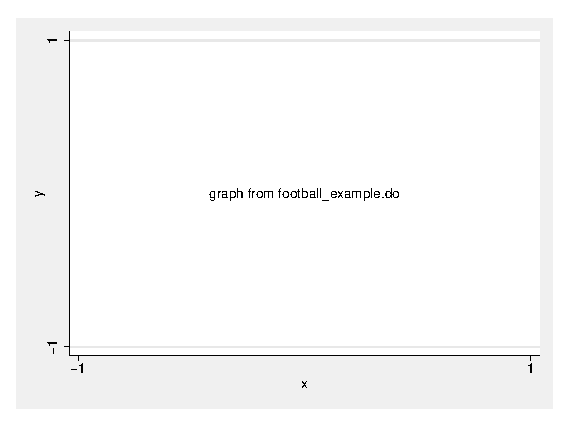
\epsfig{file=eps/3/7}
    \caption{Classic, adjusted, and generalized boxplot \alert{[will be inserted after revising the boxplot program]}}
    \label{fig:football}
\end{figure}
  % Univariate robust statistics

\part{Robust regression}
\label{part2}



\chapter{Robust linear regression}
\label{chap:robreg}

This chapter is devoted to the estimation of the parameters of linear
regression models. Let us first precise some notations.

\section{The linear regression model}

In a linear regression model, we try to explain a variable $y$---the
\emph{dependent} variable---as a linear function of some \emph{explanatory}
variables (or \emph{predictors}) $x_{1}, \dots, x_{p}$: we assume that
%
\begin{equation}
    \label{eq:linear_regr_model}
    y = \beta_{0} + \beta_{1}x_{1} + \dots + \beta_{p}x_{p} + \varepsilon
\end{equation}
%
where $\beta_{0}, \beta_{1}, \dots, \beta_{p}$ are unknown regression
coefficients---$\beta_{0}$ is called the \emph{intercept} and $\beta_{1},
\dots, \beta_{p}$ are the \emph{slopes}---that have to be estimated and
$\varepsilon$ is a random error term (the error of the statistical model, due
to omitted factors, errors of measurement, random effects, etc.).

To estimate the regression coefficients, we need a random sample of
realizations of $(y_{i}, x_{i1}, \ldots, x_{ip})$, $i=1, \dots, n$, where $n$
is the sample size. We have
%
\begin{equation}
    \label{eq:linear_regr_model_sample}
    y_{i} = \beta_{0} + \beta_{1}x_{i1} + \dots + \beta_{p}x_{ip} + \varepsilon_{i},
    \qquad i = 1, \dots, n
\end{equation}
%
where $\varepsilon_{i}$'s are generally assumed to be i.i.d.\ random variables.
That is,
\[
    \varepsilon_{i} \stackrel{\text{i.i.d.}}{\sim} F_{0, \sigma}
\]
where distribution $F_{0, \sigma}$ has a location (centrality) parameter equal
to zero and a scale parameter equal to $\sigma$.

Denoting by $\stvec{x}_{i}$ and $\boldsymbol\beta$ the $(p+1)$ dimensional
column vectors with coordinates $(1, x_{i1}, \dots, x_{ip})$ and $(\beta_{0},
\beta_{1}, \dots, \beta_{p})$, respectively, equation
(\ref{eq:linear_regr_model_sample}) can be more compactly written as
%
\begin{equation}
    \label{eq:linear_regr_model_sample_bis}
    y_{i} = \stvec{x}_{i}^t\boldsymbol\beta + \varepsilon_{i},
    \qquad i = 1, \dots, n.
\end{equation}
%
Furthermore, letting $\stvec{y} = (y_{1}, \dots, y_{n})^t$,
$\boldsymbol\varepsilon = (\varepsilon_{1}, \dots, \varepsilon_{n})^t$ and
\[
    \stmat{X} = 
    \begin{bmatrix}
        1       & x_{11} & \dots & x_{1p} \\
        1       & x_{21} & \dots & x_{2p} \\
        \vdots  & \vdots & \dots & \vdots \\
        1       & x_{n1} & \dots & x_{np}
    \end{bmatrix}
    = 
    \begin{bmatrix}
        \stvec{x}_{1}^t \\
        \stvec{x}_{2}^t \\
        \vdots         \\
        \stvec{x}_{n}^t
    \end{bmatrix}
\]
equations (\ref{eq:linear_regr_model_sample_bis}) takes the matrix-notation form
\[
    \stvec{y} = \stmat{X}\boldsymbol\beta + \boldsymbol\varepsilon.
\]

Let us note here that, \emph{conditionally to the predictors}, the linear
regression model (\ref{eq:linear_regr_model_sample_bis}) may be considered as a
location-scale model. Indeed, under the assumption of homoscedasticity---an
identical scale parameter $\sigma$ for each error term
$\varepsilon_{i}$---regression model (\ref{eq:linear_regr_model_sample_bis})
may be formulated as follows:
%
\begin{equation}
    \label{eq:location_scale_regr_model}
    y_{i} = \stvec{x}_{i}^t\boldsymbol\beta + \sigma\nu_{i}, 
    \qquad i = 1, \dots, n
\end{equation}
%
where the $\nu_{i}$'s are i.i.d.\ with distribution function $F_{0,1}$ (a
distribution with a location parameter equal to zero and a scale parameter
equal to one). In this case, the conditional distribution of $y_{i}$ given
$\stvec{x}_{i}$ is of the form:
%
\begin{equation}
    \label{eq:distr_function_yi}
    F_{y_{i} | \stvec{x}_{i}}(y) 
    = \Pr(y_{i} \leq y | \stvec{x}_{i}) 
    = \Pr\left(\nu_{i} \leq \frac{y - \stvec{x}_{i}^t\boldsymbol\beta}{\sigma} \bigg| \stvec{x}_{i}\right)
    = F_{0,1}\left(\frac{y - \stvec{x}_{i}^t\boldsymbol\beta}{\sigma}\right)
\end{equation}
%
Furthermore, if $f_{0,1}$ denotes the density function of the error terms 
$\nu_{i}$, that is,
\[
    f_{0,1}(u) = \frac{d F_{0,1}(u)}{d u} = F_{0,1}'(u)
\]
then
%
\begin{equation}
    \label{eq:dens_function_yi}
    f_{y_{i} | \stvec{x}_{i}}(y) 
    = \frac{1}{\sigma} f_{0,1}\left(\frac{y - \stvec{x}_{i}^t\boldsymbol\beta}{\sigma}\right).
\end{equation}
%
Hence, $\stvec{x}_{i}^t\boldsymbol\beta$ corresponds to the unknown location
parameter of the distribution of $y_{i}$ and $\sigma$ is the scale parameter of
the distribution of $y_{i}$. For simplicity, we will consider that the
distribution $F_{0,1}$ is continuous and symmetric around zero (and exception
is Section \ref{sec:inference}).

\begin{stremark}
The classic \emph{location-scale model} may be seen as a particular case of
regression model (\ref{eq:location_scale_regr_model}). It suffices to set
$\beta_{1} = \dots = \beta_{p} = 0$ and to assume that the $\nu_{i}$'s are
i.i.d.\ with distribution $F_{0,1}$ (such that $E(\nu_{i})=0$). In this case,
the observations
%
\begin{equation}
    \label{eq:location_scale_model}
    y_{i} = \beta_{0} + \sigma\nu_{i},
    \qquad i=1, \dots, n,
\end{equation}
%
are i.i.d.\ with a common distribution $F$ characterized by mean $\mu =
\beta_{0}$ and scale parameter $\sigma$.
\end{stremark}

\begin{stremark}
Most textbook presentations of the linear regression model assume the
explanatory variables to be fixed (and measured without error). That is, the
explanatory variables are not assumed to be random variables. In the context of
a \emph{designed experiment}, this assumption is reasonable since the values of
the experimental factors are determined \emph{a priori} by the researchers. In
other contexts such as, for example, when using social-science survey data, the
assumption makes no sense. 
    \todo{Say here what the consequence is: The fact that the $X$'s are random
    doesn't really change anything. (unlike measurement error which attenuates
    the estimates)}

Nonetheless, since we focus on the problem of outlying values, we will ignore
the issue in this chapter and consider $x_{ij}$, $i = 1, \dots, n$, $j = 1,
\dots, p$, as predetermined. That is, results will always be conditional on the
particular \emph{values} taken by the explanatory variables.
    \todo{I'm not sure whether this remark makes sense. First, LS results are
    valid also if the $X$'s are random. Second, if we talk about $X$ outliers
    it makes not much sense to assume $X$ fixed.}
\end{stremark}


\section{Different types of outliers}

Model (\ref{eq:linear_regr_model}) assume that \emph{all} units of the
population and, \emph{de facto}, all units of the sample are consistent with
the supposed linear model. If a unit has a behavior that does not respect the
underlying theoretical model, we define it as an \emph{outlying} unit with
respect to the model.

Of course, in the case of \emph{simple} linear regression model ($p=1$), a
visual inspection of the scatterplot is generally sufficient to detect the
outliers. But, when the number of explanatory variables is greater than two,
it becomes impossible to visualize all the data set and the use of robust
methods to estimate the regression parameters is then essential. More
precisely, we aim at developing procedures that provide a good fit to the bulk
of the data without being perturbed by a small proportion of outliers, and
that do not require deciding previously which observations are outliers.
Moreover, the comparison between the estimations provided by the classical
least squares estimator and those obtained using a robust estimation procedure
will allow to bring to the fore the outlyingness of some data.

In cross-sectional regression analysis, three types of outliers may influence
the estimations. \citet{rousseeuw:leroy:1987} define them as \emph{vertical
outliers}, \emph{good leverage points} and \emph{bad leverage points}. To
illustrate this terminology, consider a simple linear regression as shown in
figure~\ref{fig:outlier_types} (the generalization to higher dimensions is
straightforward). \emph{Vertical outliers} are those observations that have
outlying values for the corresponding error term (that is, in the
$y$-dimension) but are not outlying in the space of explanatory variables (in
the $x$-dimension). \emph{Good leverage points} are observations that are
outlying in the space of explanatory variables but that are located close to
the regression hyperplane. Finally, \emph{bad leverage points} are observations
that are both outlying in the space of explanatory variables and located far
from the true regression hyperplane.


\begin{figure}[h!]
    \centering
    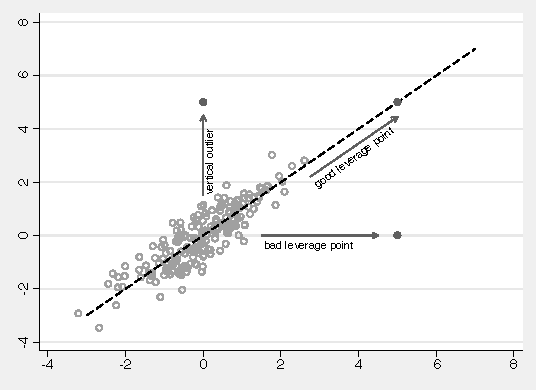
\epsfig{file=eps/4/1}
    \caption{Vertical outlier, good leverage point and bad leverage point}
    \label{fig:outlier_types}
\end{figure}

All these types of outliers risk to affect the estimation of the regression
hyperplane but their effect changes according to the estimator we will
consider and the type of outlyingness. For the classical least squares
estimation method, for instance, the bad leverage points are considered as the
most dangerous outliers because their presence can change the sign of the
slope of the regression line (in simple regression); the good leverage points
have little influence on the estimation of the regression coefficients but
they have an impact on the variances and covariances of the regression
coefficients' estimators and, consequently, risk to influence the inferential
procedures (tests and confidence intervals).

The most popular estimation method in linear regression is certainly the
\emph{least squares} (\stsc{LS}) method introduced in 1805 by Legendre.          \todo{Please provide citation details!}
One of its principal advantage is the simplicity of the
computation of the \stsc{LS} estimates. Its popularity has also be reinforced
by the fact that, under the normality of the error terms, \stsc{LS} estimates
of the regression coefficients coincide with the maximum likelihood estimates.
We will first briefly review the logic behind least squares (\stsc{LS})
estimation and recall why the \stsc{LS} estimator is particularly affected by
the presence of atypical individuals. We will thereafter introduce some
alternative estimation methods that have been proposed to try to cope with
outliers.


\section{LS estimation}

Let us denote by $\sthat{y}_{i}(\boldsymbol\beta)$ the value fitted by the
regression model for the $i$th statistical unit of the sample when taking
$\boldsymbol\beta$ as value for the vector of regression coefficients:
\[
    \sthat{y}_{i}(\boldsymbol\beta)  = \stvec{x}_{i}^t\boldsymbol\beta, 
    \qquad i = 1, \dots, n
\]
The difference between the observed value $y_{i}$ and the fitted value
$\sthat{y}_{i}(\boldsymbol\beta)$ is the residual $r_{i}(\boldsymbol\beta)$:
\[
    r_{i}(\boldsymbol\beta) = y_{i} - \sthat{y}_{i}(\boldsymbol\beta),
    \qquad i = 1, \dots, n.
\]

Although $\boldsymbol\beta$ can be estimated in several ways, the underlying
idea is often to take an estimate $\sthat{\boldsymbol\beta}$ in such a way that
the fitted values $\sthat{y}_{i}(\sthat{\boldsymbol\beta})$ for the dependent
variable are as close as possible to the observed values $y_{i}$ ($i = 1,
\dots, n$), i.e., in such a way that we minimize globally the magnitude of the
residuals $r_{i}(\sthat{\boldsymbol\beta})$. This idea leads to try to find the
estimate $\sthat{\boldsymbol\beta}$ that minimizes a specific aggregate
prediction error.

In the case of the well-known ordinary least squares (\stsc{LS}), this
aggregate prediction error is defined as the sum of squared residuals:
%
\begin{equation}\label{eq:LS_min}
    \sthat{\boldsymbol\beta}_{\stsc{LS}} = \argmin_{\boldsymbol\beta} 
    \sum_{i=1}^{n} r_{i}^{2}(\boldsymbol\beta)
\end{equation}
%
where “$\argmin$” stands for “the value minimizing”. In other terms,
$\sthat{\boldsymbol\beta}_{\stsc{LS}}$ is solution of the so called
\emph{normal equations} system --- we will also call it the \emph{estimating
equations} system --- obtained by differentiating the function $\sum_{i=1}^{n}
r_{i}^{2}(\boldsymbol\beta)$ to minimize with respect to each component of
$\boldsymbol\beta$, that is, $\sthat{\boldsymbol\beta}_{\stsc{LS}}$ is the
solution of
%
\begin{equation}\label{eq:LS_equations}
    \sum_{i=1}^{n}  r_{i}(\boldsymbol\beta)\stvec{x}_{i} = \stvec{0}
\end{equation}
%
which is equivalent to the linear equations system
\[
    \stmat{X}^t\stmat{X}\boldsymbol\beta = \stmat{X}^t\stvec{y}.
\]
If $\stmat{X}$ has full rank\footnote{The matrix of predictors $\stmat{X}$ is
said to have \emph{full rank} if its columns are linearly independent (absence
of multicollinearity), that is, if $\stmat{X}\stvec{a}\neq\stvec{0}$ for all
$\stvec{a}\neq\stvec{0}$. This is equivalent to the nonsingularity of
$\stmat{X}'\stmat{X}$.}, then the solution of (\ref{eq:LS_equations}) is unique
and is given by
%
\begin{equation}\label{eq:LS_estimator}
    \sthat{\boldsymbol\beta}_{\stsc{LS}}
    = \sthat{\boldsymbol\beta}_{\stsc{LS}}(\stmat{X}, \stvec{y})
    = (\stmat{X}^t\stmat{X})^{-1} \stmat{X}^t\stvec{y}.
\end{equation}
%
This estimate can be computed in Stata using the \stcmd{regress} command (see
\rref{regress}).

Note here that, if the model contains a constant term $\beta_{0}$, that is, if
the first component of the vectors $\stvec{x}_{i}$, $i = 1, \dots, n$, is equal
to one, it follows from (\ref{eq:LS_equations}) that the residuals
$r_{i}(\sthat{\boldsymbol\beta}_{\stsc{LS}})$, $i = 1, \dots, n$, have zero
average.

It is easy to verify that the \stsc{LS} estimator satisfies 
(see \citealp[92]{maronna:etal:2006})
%
\begin{align}
    \label{eq:regression_equivariance}
    \sthat{\boldsymbol\beta}_{\stsc{LS}}(\stmat{X},\stvec{y}+\mathbf{X}\boldsymbol\gamma) 
        &= \sthat{\boldsymbol\beta}_{\stsc{LS}}(\stmat{X},\stvec{y})+\boldsymbol\gamma
        \qquad\text{for all $\boldsymbol\gamma\in\mathbb{R}^{p+1}$} \\
    \label{eq:scale_equivariance}
    \sthat{\boldsymbol\beta}_{\stsc{LS}}(\stmat{X},\lambda\stvec{y})
        &= \lambda\sthat{\boldsymbol\beta}_{\stsc{LS}}(\stmat{X}, \stvec{y})
        \qquad\text{for all $\lambda\in\mathbb{R}$}
\end{align}
%
and, for any nonsingular $(p+1) \times (p+1)$ matrix $\stmat{A}$,
%
\begin{equation}\label{eq:affine_equivariance}
    \sthat{\boldsymbol\beta}_{\stsc{LS}}(\stmat{X}\stmat{A},\stvec{y})
    = \stmat{A}^{-1}\sthat{\boldsymbol\beta}_{\stsc{LS}}(\stmat{X},\stvec{y}).
\end{equation}
%
The properties (\ref{eq:regression_equivariance}),
(\ref{eq:scale_equivariance}) and (\ref{eq:affine_equivariance}) are called
\emph{regression}, \emph{scale} and \emph{affine equivariance} of
$\sthat{\boldsymbol\beta}_{\stsc{LS}}$, respectively. In the sequence, it will
be desirable that every other estimator of $\boldsymbol\beta$ also satisfies
these natural properties.

It is also well known that the \stsc{LS} estimator of $\boldsymbol\beta$ coincides
with the maximum likelihood estimator in case of normally distributed error
terms in (\ref{eq:linear_regr_model_sample}). Hence, $\widehat
{\boldsymbol\beta}_{\stsc{LS}}$ is the most efficient estimator of
$\boldsymbol\beta$ in the Gaussian regression model.

However, an important drawback of \stsc{LS} is that, by considering squared
residuals, it tends to award an excessive importance to observations with large
residuals and, consequently, distort parameters estimation when outliers exist.

\section{M estimation}

\subsection{L\textsubscript{1} or Least Absolute Deviation (LAD) estimation}

\citet{edgeworth:1887} realized that due to the squaring of the residuals,
\stsc{LS} becomes extremely vulnerable to the presence of outliers. To cope
with this, he proposed a method consisting in minimizing the sum of the
absolute values of the residuals rather than the sum of their squares. More
precisely, his method defines the $L_{1}$ or \emph{least absolute deviation}
(\stsc{LAD}) estimate as
%
\begin{equation}\label{eq:L1_min}
    \sthat{\boldsymbol\beta}_{\stsc{LAD}} 
        = \argmin_{\boldsymbol\beta} \sum_{i=1}^{n} |r_{i}(\boldsymbol\beta)|.
\end{equation}
%
This estimate is solution of the estimating equations system obtained by
differentiating the sum of the absolute values of the residuals with respect
to each component of $\boldsymbol\beta$:
%
\begin{equation}\label{eq:L1_equations}
    \sum_{i=1}^{n}\sign(r_{i}(\sthat{\boldsymbol\beta}_{\stsc{LAD}})) 
    \stvec{x}_{i} = \stvec{0}
\end{equation}
%
If the model contains an intercept term, (\ref{eq:L1_equations}) implies that
the residuals $r_{i}(\sthat{\boldsymbol\beta}_{\stsc{LAD}})$, $i = 1, \dots,
n$, have a median equal to zero; this motivates the fact that the \stsc{LAD}
regression estimator is also sometimes called the \emph{median regression
estimator}.

Unlike for $\sthat{\boldsymbol\beta}_{\stsc{LS}}$, there is no explicit
expression for $\sthat{\boldsymbol\beta}_{\stsc{LAD}}$.\footnote{Note also that
the \stsc{LAD} estimate of $\boldsymbol\beta$ may not be unique and has the
property that at least $(p+1)$ residuals are equal to zero.} However, there
exist very fast algorithms to compute it and
$\sthat{\boldsymbol{\beta}}_{\stsc{LAD}}$ is available in Stata via the
\stcmd{qreg} command as a standard function (see \rref{qreg}).

Finally, it can easily be seen from (\ref{eq:L1_min}) and
(\ref{eq:L1_equations}) that this estimator does protect against vertical
outliers (but not against bad leverage points). However, this gain in
robustness with respect to the \stsc{LS} estimator comes with an important loss
of efficiency: the asymptotic relative efficiency of
$\sthat{\boldsymbol{\beta}}_{\stsc{LAD}}$ with respect to
$\sthat{\boldsymbol\beta}_{\stsc{LS}}$ is equal to $2/\pi = 63.7\%$ at a
Gaussian error distribution (see \citealp{huber:1981}).

\subsection{The principle of M estimation}

\citet{huber64} hence generalized median regression to a wider class of
estimators, called \stsc{M} estimators, by considering other functions than
the absolute value in (\ref{eq:L1_min}) in order to find a reasonable balance
between robustness and Gaussian efficiency.

An \stsc{M} estimate $\sthat{\boldsymbol\beta}_{\stsc{M};\rho}$ of
$\boldsymbol\beta$ is defined by
%
\begin{equation}
    \label{eq:M_min}
    \sthat{\boldsymbol\beta}_{\stsc{M};\rho} 
        = \argmin_{\boldsymbol\beta}\sum_{i=1}^{n} 
            \rho\left(\frac{y_{i} - \stvec{x}_{i}^t\boldsymbol\beta}{\sthat{\sigma}}\right)
        = \argmin_{\boldsymbol\beta}\sum_{i=1}^{n}
            \rho\left(\frac{r_{i}(\boldsymbol\beta)}{\sthat{\sigma}}\right)
\end{equation}
%
where $\rho(u)$ is a loss function that is positive, even such that $\rho(0) =
0$, and non decreasing for positive values $u$, and $\sthat{\sigma}$ is an
auxiliary estimate of the scale parameter $\sigma$ required to standardize the
residuals and to make $\sthat{\boldsymbol\beta}_{\stsc{M};\rho}$ scale
equivariant; see (\ref{eq:scale_equivariance}). In most situations,
$\sthat{\sigma}$ is computed in advance, but it can also be computed
simultaneously through a scale \stsc{M} estimating equation. This problem will
be discussed in more details later.

\begin{stremark}
The \stsc{LS} estimate and the \stsc{LAD} estimate correspond respectively to
$\rho(u) = u^{2}$ and $\rho(u) = |u|$. In these two cases, $\sthat{\sigma}$
becomes a constant factor outside the summation sign in (\ref{eq:M_min}) and
\[
    \argmin_{\boldsymbol\beta} \sum_{i=1}^{n} \rho\left(\frac{r_{i}(\boldsymbol\beta)}{\sthat{\sigma}}\right)
    = \argmin_{\boldsymbol\beta}\sum_{i=1}^{n}\rho(r_{i}(\boldsymbol\beta)).
\]
Thus neither the \stsc{LS} nor the \stsc{LAD} estimate require an auxiliary
scale estimate.
\end{stremark}

Of course, if we want a \stsc{M} estimator more robust against vertical
outliers than the \stsc{LS} estimator, we have to take a loss function $\rho$
that is less rapidly increasing than the square function in order to give less
weight to big (in absolute value) residuals in the minimization problem. In
order to combine robustness and efficiency under a Gaussian error distribution,
\citet{huber64} has suggested to use for $\rho$ a function of the form (see
figure~\ref{fig:rho_psi_Huber}):
\[
    \rho_{\kappa}^{\stsc{H}}(u) = 
    \begin{cases}
        u^{2}                    & \text{if $|u| \leq \kappa$}\\
        2\kappa |u| - \kappa^{2} & \text{if $|u| > \kappa$}
    \end{cases}
\]
where $\kappa$ is a constant determining the trade-off between robustness and
efficiency. These functions of Huber are convex on the whole real line and may
be seen as intermediate functions between the quadratic function (leading to
the non robust but efficient \stsc{LS} estimate) and the absolute value function
(associated with the robust but poorly efficient \stsc{LAD} estimate).

Another class of loss functions $\rho$ widely used in the literature is the
class of the Tukey-Biweight                                                     \todo{Please provide citation!} 
functions (see figure~\ref{fig:rho_psi_Biweight})
%
\begin{equation}
    \label{eq:Tukey_Biweight_function}
    \rho_{\kappa}^{\stsc{B}}(u) = 
        \begin{cases}
            \frac{\kappa^{2}}{6} \left[1 - \left(1 - \left(\frac{u}{\kappa}\right)^{2}\right)^{3}\right] 
                & \text{if $|u| \leq \kappa$}\\
            \frac{\kappa^{2}}{6} 
                & \text{if $|u| > \kappa$}
        \end{cases}
\end{equation}
%
These functions are bounded. Once again, the constant $\kappa$ allows the
trade-off between robustness and Gaussian efficiency. We will show the
advantage and disadvantage to use a bounded function $\rho$ hereafter.

We may also characterize $\sthat{\boldsymbol\beta}_{\stsc{M};\rho}$ as a
solution of the estimating equations system obtained by differentiating the
function to minimize in (\ref{eq:M_min}) with respect to each component of
$\boldsymbol\beta$, that is, as a solution of the equations system
%
\begin{equation}\label{eq:M_equations}
    \sum_{i=1}^{n} \psi\left(\frac{r_{i}(\boldsymbol\beta)}{\sthat{\sigma}}\right) \stvec{x}_{i} = \stvec{0}
\end{equation}
%
where $\psi(u) = d\rho(u) / du = \rho'(u)$. For instance, taking
$\rho(u)=\rho_{\kappa}^{\stsc{H}}(u)$, we have
\[
    \psi_{\kappa}^{\stsc{H}}(u) = 
    \begin{cases}
        -2\kappa    & \text{if $u<-\kappa$}\\
        2u          & \text{if $-\kappa\leq u\leq\kappa$}\\
        2\kappa     & \text{if $u>\kappa$}
    \end{cases}
\]
for $\rho(u) = \rho_{\kappa}^{\stsc{B}}(u)$, we obtain
\[
    \psi_{\kappa}^{\stsc{B}}(u) =
    \begin{cases}
        u\left(1 - \left(\frac{u}{\kappa}\right)^{2}\right)^{2} & \text{if $|u| \leq \kappa$}\\
        0                                                       & \text{if $|u| > \kappa$}
    \end{cases}
\]
(see figures \ref{fig:rho_psi_Huber} and \ref{fig:rho_psi_Biweight}). If the
loss function $\rho$ is convex on $\mathbb{R}$---this is the case for
$\rho_{\kappa}^{\stsc{H}}$---the score function $\psi$ is monotone (non
decreasing) on $\mathbb{R}$ and $\sthat{\boldsymbol\beta}_{\stsc{M};\rho}$ is
called a \emph{monotone} regression \stsc{M} estimator; if $\rho$ is
bounded---this is the case for $\rho_{\kappa}^{\stsc{B}}$---the score function
$\psi$ vanishes out of a certain interval of $\mathbb{R}$ and
$\sthat{\boldsymbol\beta}_{\stsc{M};\rho}$ is then called a \emph{redescending}
regression \stsc{M} estimator.


\begin{figure}[h!]
    \centering
    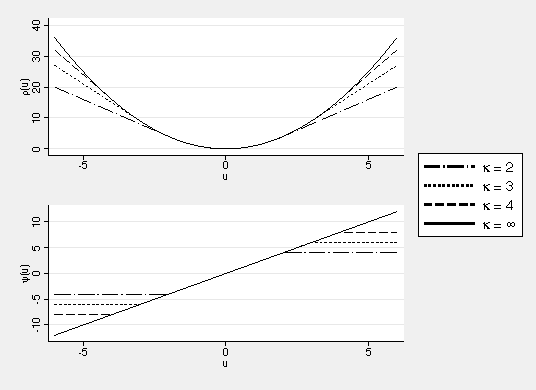
\epsfig{file=eps/4/2}
    \caption{Huber loss function $\rho_{\kappa}^{\stsc{H}}$ and score function $\psi_{\kappa}^{\stsc{H}}$}
    \label{fig:rho_psi_Huber}
\end{figure}

\begin{figure}[h!]
    \centering
    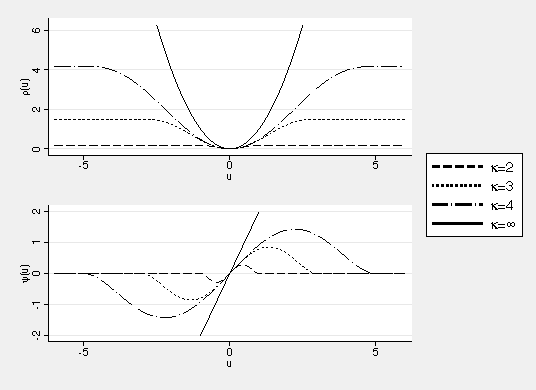
\epsfig{file=eps/4/3}
    \caption{Tukey-Biweight loss function $\rho_{\kappa}^{\stsc{B}}$ and score function $\psi_{\kappa}^{\stsc{B}}$}
    \label{fig:rho_psi_Biweight}
\end{figure}

The main advantage of monotone score functions $\psi$ is that all solutions of
(\ref{eq:M_equations}) are solutions of (\ref{eq:M_min}). In the case of
redescending score functions $\psi$, the estimating equations
(\ref{eq:M_equations}) may have multiple solutions corresponding to multiple
local minima of $\sum_{i=1}^{n}\rho(r_{i}(\boldsymbol\beta)/\sthat{\sigma})$,
and generally only one of them (the “good” solution) corresponds to the global
minimizer $\sthat{\boldsymbol\beta}_{\stsc{M};\rho}$ defined by
(\ref{eq:M_min}), which makes the computation of the \stsc{M} estimate
considerably more complex.

\begin{stremark}
Applying the \stsc{M} estimation procedure in the particular case of the
location-scale model (\ref{eq:location_scale_model}) leads to the \stsc{M}
\emph{estimators of location and scale}---we just mentioned the existence of
these estimators in the previous chapter. The interested reader will find some
results relative to these specific estimators in appendix
\ref{sec:robreg:appendix1} at the end of this chapter.
\end{stremark}

\subsection{M estimation as a generalization of maximum likelihood (ML) estimation}

The \stsc{M} estimation as defined above may be seen, as already explained, as
a generalization of the \stsc{LS} or \stsc{LAD} estimation, but also as a
generalization of the maximum-likelihood (\stsc{ML}) estimation (see, for
instance, \citealp{maronna:etal:2006}). Indeed, assuming model
(\ref{eq:location_scale_regr_model}) with fixed $\stvec{x}_{i}$ and with
$\nu_{i}$, $i = 1, \dots, n$, i.i.d.\ of density $f_{0,1}$, the likelihood of
the sample $\{y_{1}, \dots, y_{n}\}$ is given by                                \todo{Couldn't we also just use unspecified $f$ instead of $f_{0,1}$?}
\[
    \frac{1}{\sigma^{n}}\prod\limits_{i=1}^{n}
    f_{0,1}\left(\frac{y_{i}-\stvec{x}_{i}^t\boldsymbol\beta}{\sigma}\right).
\]
Hence, maximum likelihood estimation of the parameters $\boldsymbol\beta$
and $\sigma$ consists in looking for
%
\begin{align}
    \left(\sthat{\boldsymbol\beta}_{\stsc{ML}}^t,\sthat{\sigma}_{\stsc{ML}}\right)^t
    &= \arg\max_{\boldsymbol\beta,\sigma} \frac{1}{\sigma^{n}} \prod\limits_{i=1}^{n}
        f_{0,1}\left(\frac{y_{i}-\stvec{x}_{i}^t\boldsymbol\beta}{\sigma}\right)
    \nonumber\\
    &= \arg\max_{\boldsymbol\beta,\sigma} \left[\sum_{i=1}^{n}
        \ln f_{0,1}\left(\frac{y_{i}-\stvec{x}_{i}^t\boldsymbol\beta}{\sigma}\right) - n\ln\sigma\right]
    \nonumber\\
    & = \argmin_{\boldsymbol\beta,\sigma} \left[\sum_{i=1}^{n}
        \rho_{\stsc{ML}}\left(\frac{r_{i}(\boldsymbol\beta)}{\sigma}\right) + n\ln\sigma\right]
    \label{eq:ML_beta_sigma_min}
\end{align}
%
where $\rho_{\stsc{ML}}(u) = -\ln f_{0,1}(u)$. If $\sigma$ is known, the
minimization problem simply becomes
%
\begin{equation}\label{eq:ML_beta_min}
    \sthat{\boldsymbol\beta}_{\stsc{ML}} 
        = \argmin_{\boldsymbol\beta}\sum_{i=1}^{n} 
            \rho_{\stsc{ML}}\left(\frac{r_{i}(\boldsymbol\beta)}{\sigma}\right)
\end{equation}
%
and $\sthat{\boldsymbol\beta}_{\stsc{ML}}$ is solution of the estimating
equations system
\[
    \sum_{i=1}^{n} \psi_{\stsc{ML}}\left(\frac{r_{i}(\boldsymbol\beta)}{\sigma}\right) \stvec{x}_{i} = \stvec{0}
\]
where $\psi_{\stsc{ML}}(u) = \rho_{\stsc{ML}}'(u) = - (1/f_{0,1}(u))
f_{0,1}'(u)$. If $f_{0,1}$ is the standard normal density function,
$\sthat{\boldsymbol\beta}_{\stsc{ML}}$ coincides with
$\sthat{\boldsymbol\beta}_{\stsc{LS}}$. If $f_{0,1}$ is the density function of
the Laplace distribution, that is, if $f_{0,1}(u) =
\frac{1}{\sqrt{2}}\exp(-\sqrt{2}|u|)$, $u\in\mathbb{R}$, then
$\sthat{\boldsymbol\beta}_{\stsc{ML}}$ is equal to
$\sthat{\boldsymbol\beta}_{\stsc{LAD}}$.

If $\sigma$ is not known but is estimated beforehand and fixed in
(\ref{eq:ML_beta_min}), the estimating equations system becomes
\[
    \sum_{i=1}^{n} \psi_{\stsc{ML}}\left(\frac{r_{i}(\boldsymbol\beta)}{\sthat{\sigma}}\right) \stvec{x}_{i} = \stvec{0}
\]
Note that, if $\boldsymbol\beta$ and $\sigma$ are estimated simultaneously,
the estimating equations system related to (\ref{eq:ML_beta_sigma_min}) is
%
\begin{equation}\label{eq:ML_beta_sigma_equations}
    \begin{cases}
        \sum\limits_{i=1}^{n} \psi_{\stsc{ML}}\left(\frac{r_{i}(\boldsymbol\beta)}{\sigma}\right) \stvec{x}_{i} = \stvec{0}\\
        \frac{1}{n} \sum\limits_{i=1}^{n} \rho_{\stsc{ML};\mathrm{scale}}\left(\frac{r_{i}(\boldsymbol\beta)}{\sigma}\right) = \delta
    \end{cases}
\end{equation}
%
where $\rho_{\stsc{ML};\mathrm{scale}}(u) = u\psi_{\stsc{ML}}(u)$ and
$\delta=1$.

\subsection{Practical implementation of M estimates}
\label{subsec:practical_implementation_Mestimate}

Let us first assume, for simplicity, that the scale parameter $\sigma$ is
known. In that case, the regression M-estimate
$\sthat{\boldsymbol\beta}_{\stsc{M};\rho}$ is solution of the estimating
equations system (\ref{eq:M_equations}) where $\sthat{\sigma}$ is replaced by
$\sigma$. Defining the weight function $w$ by
\[
    w(u) = 
    \begin{cases}
        \frac{\psi(u)}{u} & \text{if $u\neq0$}\\
        \psi'(0)          & \text{if $u=0$}
    \end{cases}
\]
the estimating system (\ref{eq:M_equations}) can be rewritten as
%
\begin{equation}\label{eq:weighted_LS_equations}
    \sum_{i=1}^{n} w_{i} r_{i}(\boldsymbol\beta) \stvec{x}_{i} = \stvec{0}
\end{equation}
%
where $w_{i} = w(r_{i}(\boldsymbol\beta)/\sigma)$. Hence, the equations to
solve in the \stsc{M} estimation procedure appear as \emph{weighted} versions
of the normal equations (\ref{eq:LS_equations}) related to \stsc{LS}
estimation, and if the $w_{i}$'s were known, the equations
(\ref{eq:weighted_LS_equations}) could be solved by applying \stsc{LS} to
$\sqrt{w_{i}}y_{i}$ and $\sqrt{w_{i}}\stvec{x}_{i}$. But the weights $w_{i}$
are functions of $\boldsymbol\beta$ and depend upon the data, and hence are not
known. So we have to use an iterative procedure. Using an initial estimate
$\sthat{\boldsymbol\beta}_0$ for $\boldsymbol\beta$ (for instance, the
\stsc{LAD} estimate of $\boldsymbol\beta$), the weights can be computed and
serve as the start of an \emph{iteratively reweighted least squares algorithm}
(\stsc{IRWLS}). Note however that the latter is guaranteed to converge to the
global minimum of (\ref{eq:M_min}) only if the loss function $\rho$ is convex
on the whole real line $\mathbb{R}$ (which is the case for the
$\rho_{c}^{\stsc{H}}$ functions introduced by Huber).\footnote{In the case of
a convex loss function $\rho$, the convergence of the algorithm to the global
minimum of (\ref{eq:M_min}) is guaranteed whatever the starting point
$\sthat{\boldsymbol\beta}_0$.}

If $\sigma$ is not known, it can be estimated (in a robust way) beforehand
using the residuals $r_{i}(\sthat{\boldsymbol\beta}_0)$, $i = 1, \dots, n$,
and then fixed in the iterative procedure described above. It is of course
also possible to estimate simultaneously $\boldsymbol\beta$ and $\sigma$ in
this procedure, by updating $\sthat{\sigma}$ at each iteration (see
\citealp{maronna:etal:2006} for more details).

\subsubsection{Regression M estimate with preliminary scale estimation}

In practice, we may take the \stsc{LAD} estimate as initial estimate
$\sthat{\boldsymbol\beta}_0$ for $\boldsymbol\beta$ (recall that the \stsc{LAD}
estimate does not require estimating a scale). Then we may estimate $\sigma$
using normalized \stsc{MAD} of the residuals
$r_{i}(\sthat{\boldsymbol\beta}_0)$. More precisely, we may take
\[
    \sthat{\sigma} = 1.4826 \cdot 
    \med_{i}\left(\left|r_{i}(\sthat{\boldsymbol\beta}_0)\right|; r_{i}(\sthat{\boldsymbol\beta}_0) \neq 0\right).
\]
The reason for using only \emph{non null} residuals is that, since at least
$(p+1)$ residuals $r_{i}(\sthat{\boldsymbol\beta}_0) =
r_{i}(\sthat{\boldsymbol\beta}_{\stsc{LAD}})$ are equal to zero, determining
the \stsc{MAD} of the $n$ residuals could lead to underestimating $\sigma$ when
$p$ is large.

Since $\sthat{\boldsymbol\beta}_{\stsc{LAD}}$ is regression, scale and
affine equivariant, it is easy to show that
%
\begin{align*}
    \sthat{\sigma}(\stmat{X}, \stvec{y} + \stmat{X}\boldsymbol\gamma)
        &= \sthat{\sigma}(\stmat{X}, \stvec{y})
        \qquad\text{for all $\boldsymbol\gamma \in \mathbb{R}^{p+1}$}\\
    \sthat{\sigma}(\stmat{X}\stmat{A}, \stvec{y})
        &= \sthat{\sigma}(\stmat{X}, \stvec{y})
        \qquad\text{for any nonsingular $\mathbf{A} \in \mathbb{R}^{(p+1)\times(p+1)}$}
\end{align*}
%
and
\[
    \sthat{\sigma}(\stmat{X}, \lambda\stvec{y}) 
    = |\lambda| \sthat{\sigma} (\stmat{X}, \stvec{y})
    \qquad\text{for all $\lambda\in\mathbb{R}$.}
\]
Hence, $\sthat{\sigma}$ is regression and affine invariant, as well as scale
equivariant, which ensures the regression, scale end affine equivariance of
the \stsc{M} estimator $\sthat{\boldsymbol\beta}_{\stsc{M};\rho}$.


\subsection{Regression quantiles as regression M estimates}

Let
\[
    \rho_{\alpha}(u)=
    \begin{cases}
        \alpha u     & \text{if $u\geq0$}\\
        -(1-\alpha)u & \text{if $u<0$}
    \end{cases}
\]
for $\alpha \in (0,1)$. \citet{Koenker:1978} defined the \emph{regression $\alpha$-quantile} 
$\sthat{\boldsymbol\beta}_{\alpha}$ as follows:
%
\begin{equation}\label{eq:quantile_regr_min}
    \sthat{\boldsymbol\beta}_{\alpha} 
    = \argmin_{\boldsymbol\beta} \sum_{i=1}^{n} \rho_{\alpha}(y_{i}-\stvec{x}_{i}^t\boldsymbol\beta)
\end{equation}

The case $\alpha=0.5$ corresponds to the \stsc{LAD} estimate. Assume the model
\[
    y_{i} = \stvec{x}_{i}^t \boldsymbol\beta_{\alpha} + \epsilon_{i},
    \qquad i = 1, \dots, n
\]
where the $\stvec{x}_{i}$'s are fixed and the $\alpha$-quantile of
$\epsilon_{i}$ is zero; this is equivalent to assuming that the
$\alpha$-quantile of $y_{i}$ is, conditionally to $\stvec{x}_{i}$, equal to
$\stvec{x}_{i}^t\boldsymbol\beta_{\alpha}$. Then $\widehat
{\boldsymbol\beta}_{\alpha}$ defined by (\ref{eq:quantile_regr_min}) is an
estimate of $\boldsymbol\beta_{\alpha}$. It may be seen as a generalization of
the \stsc{LAD} estimate as well as a specific case of \stsc{M} estimate.

Regression quantiles are especially useful with heteroskedastic data. There is
a very large literature on regression quantiles; see, for instance,
\citet{Koenker:2005}.

\subsection{Monotone vs. redescending M estimators}

As already mentioned, taking a loss function $\rho(u)$ in the minimization
problem (\ref{eq:M_min}) that is less rapidly increasing than the square
function provides a certain robustness of the regression \stsc{M} estimate with
respect to the vertical points. But what about the robustness of
$\sthat{\boldsymbol\beta}_{\stsc{M};\rho}$ with respect to leverage points? To
answer to this question, let us recall that
$\sthat{\boldsymbol\beta}_{\stsc{M};\rho}$ is solution of the estimating
equations system (\ref{eq:M_equations}).

It is easy to see that \emph{monotone} \stsc{M} estimates break down in
presence of a single bad leverage point. Indeed, if $\psi(u)$ is a monotone
function, an $\stvec{x}$-outlier will dominate the solution of
(\ref{eq:M_equations}) in the following sense: if for some $i$, $\stvec{x}_{i}$
is “much larger than the rest”, then in order to make the sum in the left part
of (\ref{eq:M_equations}) to zero, the residual
$r_{i}(\sthat{\boldsymbol\beta}) = y_{i} -
\stvec{x}_{i}^t\sthat{\boldsymbol\beta}$ must be near zero, that is, the
regression hyperplane has to fit the point $(\stvec{x}_{i}, y_{i})$ as well as
possible, and hence $\sthat{\boldsymbol\beta}$ is essentially determined by
this leverage point $(\stvec{x}_{i}, y_{i})$.

This does not happen with the \emph{redescending} \stsc{M} estimate since the
use of a function $\psi$ that vanishes for “outlying” residuals allows to find
a solution $\widehat{\boldsymbol\beta}_{\stsc{M};\rho}$ of
(\ref{eq:M_equations}) which is not affected by the presence of a bad leverage
point $(\stvec{x}_{i}, y_{i})$ in the data set. Hence, from the robustness
point of view, the redescending regression \stsc{M} estimators are more interesting
than the monotone \stsc{M} estimators. Unfortunately, as already explained, the
practical implementation of \stsc{M} estimators is less easy for the
redescending than for the monotone ones.

\subsection{GM estimation}

Other approaches have been considered to limit the influence of leverage points
on the estimation of the regression coefficients. For instance, defining
$\underline{\stvec{x}}_{i} = (x_{i1}, \ldots, x_{ip})'$ such that
$\stvec{x}_{i} = (1,\underline{\stvec{x}}_{i}')'$, a simple way to robustify a
monotone \stsc{M} estimate is to downweight the influential
$\underline{\stvec{x}}_{i}$'s to prevent them from dominating the estimating
equations. Hence we may define an estimate as solution of
\begin{equation}\label{eq:GM_equations_1}
    \sum_{i=1}^{n} \psi\left(\frac{r_{i}(\boldsymbol\beta)}{\sthat{\sigma}}\right) 
    \widetilde{w}(d(\underline{\stvec{x}}_{i})) \stvec{x}_{i} = \stvec{0}
\end{equation}
where $\widetilde{w}$ is a weight function and $d(\underline{\stvec{x}}_{i})$
is some measure of the “largeness” of $\underline{\stvec{x}}_{i}$. Here $\psi$
is monotone and $\sthat{\sigma}$ is simultaneously estimated by an \stsc{M}
estimating equation of the form
\[
    \frac{1}{n}\sum_{i=1}^{n} \rho_{\mathrm{scale}}\left(\frac{r_{i}(\boldsymbol\beta)}{\sigma}\right)  = \delta.
\]
In order to bound the effect of influential points, $\widetilde{w}$ must be
such that $\widetilde{w}(t)t$ is bounded.

More generally, we may let the weights depend on the residuals as well as on
the predictor variables, and use a \emph{generalized} \stsc{M} estimate
(\stsc{GM} estimate) $\sthat{\boldsymbol\beta}_{\stsc{GM}}$ defined as solution
of
%
\begin{equation}\label{eq:GM_equations_2}
    \sum_{i=1}^{n}\eta\left(d(\underline{\stvec{x}}_{i}), \frac{r_{i}(\boldsymbol\beta)}{\sthat{\sigma}}\right)
    \stvec{x}_{i} = \stvec{0}
\end{equation}
%
where for each $s$, $\eta(s,u)$ is a nondecreasing and bounded $\psi$-function
of $u$. The estimating equations system (\ref{eq:GM_equations_1}) may be seen
as a particular case of (\ref{eq:GM_equations_2}) when choosing $\eta(s,u) =
\widetilde{w}(s) \psi(u)$. This particular choice corresponds to the class of
\emph{Mallows estimates} (see \citealp{Mallows:1975}) which has been
extensively studied in the literature.

The most usual way to measure the “largeness” of $\underline{\stvec{x}}_{i}$,
$i=1, \dots, n$, is to take the \emph{leverage} of $\underline{\stvec{x}}_{i}$,
that is, to consider
%
\begin{equation}
    \label{eq:leverage}
    d(\underline{\stvec{x}}_{i}) = 
    \sqrt{\left(\underline{\stvec{x}}_{i} - \sthat{\boldsymbol\mu}_{\underline{\stvec{x}}}\right)^t
    \sthat{\boldsymbol\Sigma}_{\underline{\stvec{x}}}^{-1}
    \left(\underline{\stvec{x}}_{i} - \sthat{\boldsymbol\mu}_{\underline{\stvec{x}}}\right)}
\end{equation}
%
where $\sthat{\boldsymbol\mu}_{\underline{\stvec{x}}}$ and
$\sthat{\boldsymbol\Sigma}_{\underline{\stvec{x}}}$ are a robust location
vector and robust dispersion matrix of the $\underline{\stvec{x}}_{i}$'s,
respectively (see chapter~\ref{chap:mv}). If
$\sthat{\boldsymbol\mu}_{\underline{\stvec{x}}}$ and
$\sthat{\boldsymbol\Sigma}_{\underline{\stvec{x}}}$ are the sample mean and
covariance matrix, $d(\cdot)$ is known as the Mahalanobis distance.

As stated in \citet{rousseeuw:leroy:1987}, the \stsc{GM} estimators were
constructed in the hope of bounding the influence of a single outlying
observation. Relying on this, optimal choices of $\psi$ and $\widetilde{w}$
were made (see, among others, \citealp{Ronchetti:Rousseeuw:1985} for a survey).
However, \citet{Maronna:1979} have proven that the breakdown point of all
\stsc{GM} estimators is non-zero but decreases as a function of $p$ (i.e., the
breakdown point is less or equal to $1/(p+1)$) pointing out that a
\stsc{GM} estimator is interesting to be used only when the number of
explanatory variables is very small. Furthermore, \citet{maronna:etal:2006}
show that, to obtain affine equivariance of
$\sthat{\boldsymbol\beta}_{\stsc{GM}}$, it is necessary that
$\sthat{\boldsymbol\mu}_{\underline{\stvec{x}}}$ and
$\sthat{\boldsymbol\Sigma}_{\underline{\stvec{x}}}$ used in (\ref{eq:leverage})
are affine equivariant, which presents the same computational difficulties as
for redescending \stsc{M} estimates and reduce substantially the appeal of this
estimator.

\section{Robust regression with a high breakdown point}

As explained previously, \stsc{LS} regression is now being criticized more and
more for its dramatic lack of robustness. Indeed, one single outlier can have
an arbitrarily large effect on the estimate: the breakdown point
$\varepsilon^*$ of $\sthat{\beta}_{\stsc{LS}}$ is clearly equal to zero.
Although \stsc{LAD} regression protects against outlying $y_{i}$, it cannot
cope with grossly aberrant values of $\stvec{x}_{i}$: \stsc{LAD} regression
yields the same value $\varepsilon^*=0$ as \stsc{LS}. \stsc{M} estimation
provides a certain robustness with respect to vertical points, but not with
respect to bad leverage points when the loss function $\rho$ is unbounded: the
breakdown point $\varepsilon^*$ associated with a monotone \stsc{M} estimator
is then still equal to zero.

Because of this vulnerability to bad leverage points, generalized \stsc{M}
estimators (\stsc{GM} estimators) were introduced, with the basic purpose of
bounding the influence of outlying $\stvec{x}_{i}$. It turns out, however, that
the GM-estimators now in use have a breakdown point of at most $1/(p+1)$, where
$(p+1)$ is the dimension of $\stvec{x}_{i}$. Various other estimators have been
proposed by \citet{Theil:1950}, \citet{Brown:1951}, \citet{Sen:1968},
\citet{Jaeckel:1972}, and \citet{Andrews:1974}, but none of them achieves
$\varepsilon^*=30\%$ in the case of simple regression ($p=1$).

All of this raises the question whether robust regression with a high breakdown
point is at all possible. The affirmative answer was given by
\citet{Siegel:1982}, who proposed an estimator (the \emph{repeated median})
with a 50\% breakdown point. Note that 50\% is the best that can be expected:
for larger amounts of contamination, it becomes impossible to distinguish
between the “good” and the “bad” parts of the sample. Siegel's estimator can be
calculated explicitly but is not equivariant for linear transformations of the
$\stvec{x}_{i}$ (it is not affine equivariant). This explains why we do not
study this estimator in more details and prefer to present other estimators
introduced by Rousseeuw and Yohai, and all based on a robust scale measure.

\subsection{LTS and LMS estimation}

Robustness can be achieved by tackling the estimation of the regression
parameters vector $\boldsymbol\beta$ from a different perspective. We know that
\stsc{LS} estimation is based on the minimization of the variance of the
residuals. However, since the variance is highly sensitive to outliers,
LS-estimate will be sensitive to them as well. An interesting idea would then
consist in minimizing a measure of the residual dispersion
$s(r_{1}(\boldsymbol\beta), \dots, r_{n}(\boldsymbol\beta))$ that is less
sensitive to extreme residuals.

Relying on this idea, \citet{Rousseeuw:1983} introduced the \emph{Least Trimmed
Sum of Squares} (\stsc{LTS}) estimator which is based on the minimization of a
trimmed variance of the residuals:
\[
    \sthat{\boldsymbol\beta}_{\stsc{LTS}}
     = \argmin_{\boldsymbol\beta}s_{\stsc{LTS}}(r_{1}(\boldsymbol\beta), \dots, r_{n}(\boldsymbol\beta))
\]
with
\[
    s_{\stsc{LTS}}(r_{1}(\boldsymbol\beta), \dots, r_{n}(\boldsymbol\beta))
    = \sqrt{\frac{1}{\lceil\alpha n\rceil} 
      \sum_{i=1}^{\lceil\alpha n\rceil}r_{(i)}^{2}(\boldsymbol\beta)}
\]
where $1/2 \leq \alpha \leq 1$ and $r_{(1)}^{2}(\boldsymbol\beta) \leq \dots
\leq r_{(n)}^{2}(\boldsymbol\beta)$ are the ordered squared residuals. The
constant $\alpha$ determines the trade-off between the robustness and the
efficiency of the estimator. Indeed, if $\alpha$ tends to one, the \stsc{LTS}
estimator tends to the \stsc{LS} estimator. In contrast, if $\alpha = 1/2$, the
\stsc{LTS} estimator will resist up to 50\% of outlying data and, consequently,
will have a breakdown point equal to 50\%. Unfortunately, even if
$\sthat{\boldsymbol\beta}_{\stsc{LTS}}$ converges to $\boldsymbol\beta$ at a
rate of $1/\sqrt{n}$, its efficiency is low (under Gaussian conditions, the
asymptotic relative efficiency of $\sthat{\boldsymbol\beta}_{\stsc{LTS}}$ with
respect to $\sthat{\boldsymbol\beta}_{\stsc{LS}}$ reaches only 7\% when 50\% of
the data are trimmed).

Despite its relatively low efficiency, the \stsc{LTS} estimator is quite popular
because it can be quickly computed using the \emph{Fast-lts algorithm}
developed by \citet{rousseeuw&vdriessen99}; this estimator is available in
Stata through the command \stcmd{robreg lts}.

Following the same idea, \citet{rousseeuw:1984} introduced the \emph{Least Median
Squares} (\stsc{LMS}) estimator based on the minimization of the median of
the squared residuals:\footnote{The variance of the residuals corresponds to
the arithmetic mean of the squared residuals; why not replace the mean by the
more robust median?}
\[
    \sthat{\boldsymbol\beta}_{\stsc{LMS}} 
    = \argmin_{\boldsymbol\beta} s_{\stsc{LMS}}(r_{1}(\boldsymbol\beta), \dots, r_{n}(\boldsymbol\beta))
\]
with
\[
    s_{\stsc{LMS}}(r_{1}(\boldsymbol\beta), \dots, r_{n}(\boldsymbol\beta)) 
    = \sqrt{\mathrm{med}_{i}\;r_{i}^{2}(\boldsymbol\beta)}.
\]
\stsc{LMS} satisfies $\varepsilon^* = 50\%$ but has unfortunately a very low
efficiency because of its $1/\sqrt[3]{n}$ convergence rate. The \stsc{LMS}
estimator is available in Stata through the command \stcmd{robreg lms}.        \todo{Add paragraph on LQS, as this is also supported by robreg.}

\subsection{S estimation}

Following always the same principle, \citet{rousseeuw:yohai:1984} have
introduced a more general class of estimators: the regression
\stsc{S} estimators.

In order to well understand the basic intuition behind the \stsc{S} estimation,
let us consider once again the \stsc{LS} estimation. For \stsc{LS} estimation,
we actually are looking for the value of the regression coefficients vector
$\boldsymbol{\beta}$ that minimizes the variance (or standard deviation) of the
residuals $r_{i}(\boldsymbol\beta)$, $i = 1, \dots, n$. More formally, we have
\[
    \sthat{\boldsymbol\beta}_{\stsc{LS}} 
    = \argmin_{\boldsymbol\beta} s_{\stsc{LS}}(r_{1}(\boldsymbol\beta), \dots, r_{n}(\boldsymbol\beta))
\]
with
\[
    s_{\stsc{LS}}(r_{1}(\boldsymbol\beta), \dots, r_{n}(\boldsymbol\beta)) 
    = \sqrt{\frac{1}{n}\sum_{i=1}^{n} r_{i}^{2}(\boldsymbol\beta)}.
\]
The dispersion measure $s_{\stsc{LS}}$ may be characterized as follows: given
the realizations $e_{1}, \dots, e_{n}$ of $n$ i.i.d.\ random variables whose
distribution is characterized by a mean equal to zero and a scale parameter
$\sigma$, the dispersion measure $s_{\stsc{LS}}(e_{1}, \dots, e_{n})$ of the
sample is an estimate of $\sigma$ satisfying the equality
\[
    \frac{1}{n}\sum_{i=1}^{n} \left(\frac{e_{i}}{s_{\stsc{LS}}(e_{1}, \dots, e_{n})}\right)^{2} = 1
\]
or, taking $\rho(u) = u^{2}$,
\[
    \frac{1}{n}\sum_{i=1}^{n} \rho\left(\frac{e_{i}}{s_{\stsc{LS}}(e_{1}, \dots, e_{n})}\right) = 1.
\]
Moreover, if $u \sim \mathcal{N}(0,1)$, then $E(\rho(u)) = E(u^{2}) = 1$.

The \stsc{S} estimation procedure proposed by \citet{rousseeuw:yohai:1984}
relies on the same philosophy as the one underlying the \stsc{LS} estimation,
but introduces robustness by using specific robust residual dispersion measures
which correspond to \stsc{M} estimators of the scale parameter $\sigma$. More
formally, given the realizations $e_{1}, \dots, e_{n}$ of $n$ i.i.d.\ random
variables with scale parameter $\sigma$ (and a location parameter equal to
zero), the \stsc{M} estimate $\sthat{\sigma}_{\rho}$ of $\sigma$ is the
measure of dispersion $s_{\rho}(e_{1}, \dots, e_{n})$ defined as the solution
of the equation
%
\begin{equation}\label{eq:M_scale_equation}
    \frac{1}{n}\sum_{i=1}^{n} \rho\left(\frac{e_{i}}{s_{\rho}(e_{1}, \dots, e_{n})}\right) = \delta
\end{equation}
%
where
\begin{itemize}
    \item the function $\rho(\cdot)$ is positive, even (such that
    $\rho(0) = 0$), non decreasing for positive values and bounded;

    \item the constant $\delta$ is defined such that $\sthat{\sigma}_{\rho} =
    s_{\rho}(e_{1}, \dots, e_{n})$ is a consistent estimate of $\sigma$ for the
    Gaussian regression model (generally $\delta$ is defined by $\delta =
    E(\rho(u))$ for $u \sim \mathcal{N}(0,1)$; the consistency parameter
    $\delta$ would therefore be nothing else than the population counterpart of
    the lefthand side of equation (\ref{eq:M_scale_equation})).
\end{itemize}

Then \citet{rousseeuw:yohai:1984} defined an \stsc{S} estimate of
$\boldsymbol\beta$ by
\[
    \sthat{\boldsymbol\beta}_{\stsc{S};\rho} 
    = \argmin_{\boldsymbol\beta}s_{\rho} (r_{1}(\boldsymbol\beta), \dots, r_{n}(\boldsymbol{\beta}))
\]
where $s_{\rho}$ is a measure of dispersion defining a scale \stsc{M} estimator, that is,
satisfying
%
\begin{equation}\label{eq:M_scale_equation_res}
    \frac{1}{n}\sum_{i=1}^{n} \rho\left(\frac{r_{i}(\boldsymbol{\beta})}%
        {s_{\rho}(r_{1}(\boldsymbol\beta), \dots, r_{n}(\boldsymbol\beta))}\right) = \delta
    \qquad\text{for all $\boldsymbol\beta \in \mathbb{R}^{p+1}$.}
\end{equation}

One important fact is that an \stsc{S} estimate of $\boldsymbol\beta$ is also an
\stsc{M} estimate. More precisely, $\sthat{\boldsymbol\beta}_{\stsc{S};\rho}$
is an \stsc{M} estimate (in the sense of \ref{eq:M_min}) in that
%
\begin{equation}\label{eq:S_Minequality_1}
    \sum_{i=1}^{n}\rho\left(\frac{r_{i}(\sthat{\boldsymbol\beta}_{\stsc{S};\rho})}{\sthat{\sigma}_{\rho}}\right) 
    \leq \sum_{i=1}^{n}\rho\left(\frac{r_{i}(\widetilde{\boldsymbol\beta})}{\sthat{\sigma}_{\rho}}\right)
    \qquad
    \text{for all $\widetilde{\boldsymbol\beta} \in \mathbb{R}^{p+1}$}
\end{equation}
%
where the residuals are standardized by the same scale \stsc{M} estimate
$\sthat{\sigma}_{\rho} =
s_{\rho}(r_{1}(\sthat{\boldsymbol\beta}_{\stsc{S};\rho}),\allowbreak
\dots,\allowbreak r_{n}(\sthat{\boldsymbol\beta}_{\stsc{S};\rho}))$ of $\sigma$
on both sides of the inequality (\ref{eq:S_Minequality_1}). Indeed,
$\sthat{\boldsymbol\beta}_{\stsc{S};\rho}$ minimizes the residual dispersion
measure $s_{\rho}(r_{1}(\boldsymbol\beta), \dots, r_{n}(\boldsymbol\beta))$
which satisfies (\ref{eq:M_scale_equation_res}). This means that, if we denote
$\sthat{\sigma}_{\rho} =
s_{\rho}(r_{1}(\sthat{\boldsymbol\beta}_{\stsc{S};\rho}), \dots,
r_{n}(\sthat{\boldsymbol\beta}_{\stsc{S};\rho}))$ and
$\widetilde{\sigma}_{\rho} = s_{\rho}(r_{1}(\widetilde{\boldsymbol\beta}),
\dots, r_{n}(\widetilde{\boldsymbol\beta}))$ for $\widetilde{\boldsymbol\beta}
\in \mathbb{R}^{p+1}$, we have $\sthat{\sigma}_{\rho} \leq
\widetilde{\sigma}_{\rho}$ and
\[
    \sum_{i=1}^{n} \rho\left(\frac{r_{i}(\sthat{\boldsymbol\beta}_{\stsc{S};\rho})}{\sthat{\sigma}_{\rho}}\right) 
    = n\delta
    = \sum_{i=1}^{n}\rho\left(\frac{r_{i}(\widetilde{\boldsymbol\beta})}{\widetilde{\sigma}_{\rho}}\right)
\]
Then, since $\rho$ is monotone and $\sthat{\sigma}_{\rho} \leq
\widetilde{\sigma}_{\rho}$, we necessarily have
\[
    \sum_{i=1}^{n} \rho\left(\frac{r_{i}(\sthat{\boldsymbol\beta}_{\stsc{S};\rho})}{\sthat{\sigma}_{\rho}}\right)
    = \sum_{i=1}^{n} \rho\left(\frac{r_{i}(\widetilde{\boldsymbol\beta})}{\widetilde{\sigma}_{\rho}}\right)
    \leq \sum_{i=1}^{n}\rho\left(\frac{r_{i}(\widetilde{\boldsymbol\beta})}{\sthat{\sigma}_{\rho}}\right)
\]
which proves (\ref{eq:S_Minequality_1}).

If $\rho$ has a derivative $\psi$, it follows that
$\sthat{\boldsymbol{\beta}}_{\stsc{S};\rho}$ is also an \stsc{M} estimate in
the sense of (\ref{eq:M_equations}), but with the condition that the scale
parameter $\sigma$ is estimated simultaneously with $\boldsymbol\beta$. More
formally, $\boldsymbol\beta$ is estimated by
$\sthat{\boldsymbol\beta}_{\stsc{S};\rho}$ and $\sigma$ by
$\sthat{\sigma}_{\rho}=s_{\rho}(r_{1}(\sthat{\boldsymbol\beta}_{\stsc{S};\rho}),
 \dots, r_{n}(\sthat{\boldsymbol\beta}_{\stsc{S};\rho}))$, with
$\sthat{\boldsymbol\beta}_{\stsc{S};\rho}$ and $\sthat{\sigma}_{\rho}$ such that
\[
    \begin{cases}
        \sum_{i=1}^{n} 
        \psi\left(\frac{r_{i}(\sthat{\boldsymbol\beta}_{\stsc{S};\rho})}{\sthat{\sigma}_{\rho}}\right) 
        \stvec{x}_{i} = \stvec{0}
        \\[1em]
        \frac{1}{n} \sum_{i=1}^{n}
        \rho\left(\frac{r_{i}(\sthat{\boldsymbol\beta}_{\stsc{S};\rho})}{\sthat{\sigma}_{\rho}}\right)
        = \delta
    \end{cases}
\]
Note that, taking $\rho(u) = u^{2}$ and $\delta=1$, we retrieve
the standard \stsc{LS} minimization problem.

The choice of $\rho(\cdot)$ is crucial to have good robustness
properties\footnote{Note that the function $\rho$ defining the \stsc{S}
estimator needs to be \emph{bounded} to get a positive breakdown point for the
regression estimator $\sthat{\boldsymbol\beta}_{\stsc{S};\rho}$.} and a high
Gaussian efficiency. The Tukey-Biweight function defined in
(\ref{eq:Tukey_Biweight_function}), with $\kappa = 1.547$, is a common choice.
This \stsc{S} estimator resists to a contamination of up to 50\% of outliers
and, hence, has a breakdown point of 50\%. Unfortunately, this \stsc{S}
estimator has a Gaussian efficiency of only 28.7\%. If $\kappa = 5.182$, the
Gaussian efficiency raises to 96.6\% but the breakdown point drops to 10\%.
Actually an \stsc{S} estimator cannot simultaneously have a high breakdown
point and a high efficiency. In particular, \citet{Hossjer:1992} has shown that the
maximum Gaussian asymptotic efficiency of an \stsc{S} estimator with a
breakdown point of 50\% is 33\%.

\subsection{MM estimation}
\label{subsec:MM_estimation}

We have just seen that \stsc{S} estimation does not allow to reach jointly a
high breakdown point and a high Gaussian efficiency. How should we then
estimate the parameters of the regression model if we aim to combine high
efficiency under normal errors with a high breakdown point? Several proposals
have been made: the \stsc{MM} estimators of \citet{yohai:1987}, the $\tau$
estimators of \citet{Yohai:1988}, the constrained \stsc{M} (\stsc{CM})
estimators of \citet{Mendes:1996}. All these estimators can have a Gaussian
asymptotic efficiency as close to 1 as desired, and simultaneously a breakdown
point of 50\%. Furthermore, \citet{Gervini:2002} proposed one estimator that
has a breakdown point of 50\% and an efficiency equal to 1.

Let us here focus our attention on the regression \stsc{MM} estimators since
they are based on the \stsc{M} and \stsc{S} estimation procedures studied in
the previous sections. An \stsc{MM} estimator is defined in two successive
steps:

\begin{enumerate}
    \item Take an \stsc{S} estimate $\sthat{\boldsymbol\beta}_{\stsc{S};\rho_{0}}$
    with high breakdown point (but possibly low Gaussian efficiency) where the scale
    measure $s_{\rho_{0}}$ is defined by
    \[
        \frac{1}{n} \sum_{i=1}^{n}\rho_{0}\left(\frac{r_{i}(\boldsymbol\beta)}
            {s_{\rho_{0}}(r_{1}(\boldsymbol\beta), \dots, r_{n}(\boldsymbol\beta))}\right) 
            = \delta
        \qquad\text{for all $\boldsymbol\beta\in\mathbb{R}^{p+1}$}
    \]
    ($s_{\rho_{0}}$ is associated with the function $\rho_{0}(\cdot)$ and the
    constant $\delta$). Let $\sthat{\sigma}_{\rho_{0}} =
    s_{\rho_{0}}(r_{1}(\sthat{\boldsymbol\beta}_{\stsc{S};\rho_{0}}),\allowbreak
    \dots,\allowbreak r_{n}(\sthat{\boldsymbol\beta}_{\stsc{S};\rho_{0}}))$.

    \item Take any other function $\rho(\cdot) \leq \rho_{0}(\cdot)$ and find
    the \stsc{MM} estimate $\sthat{\boldsymbol\beta}_{\stsc{MM};\rho_{0},\rho}$
    as a local minimum of
    %
    \begin{equation}\label{eq:MM_min}
        \sum_{i=1}^{n} \rho\left(\frac{r_{i}(\boldsymbol\beta)}{\sthat{\sigma}_{\rho_{0}}}\right)
    \end{equation}
    %
    such that
    %
    \begin{equation}\label{eq:MM_inequality}
        \sum_{i=1}^{n} \rho\left(\frac{r_{i}(\sthat{\boldsymbol\beta}_{\stsc{MM};\rho_{0},\rho})}
            {\sthat{\sigma}_{\rho_{0}}}\right)
     \leq \sum_{i=1}^{n}\rho\left(\frac{r_{i}(\sthat{\boldsymbol\beta}_{\stsc{S};\rho_{0}})}
         {\sthat{\sigma}_{\rho_{0}}}\right).
    %
    \end{equation}
    %
\end{enumerate}

The key result is given in \citet{yohai:1987}. Recall that all local minima of
(\ref{eq:MM_min}) are solutions of the estimating equations
(\ref{eq:M_equations}) with $\psi(u) = \rho^{\prime}(u)$ and $\sthat{\sigma} =
\sthat{\sigma}_{\rho_{0}}$:
%
\begin{equation}\label{eq:MM_equations}
    \sum_{i=1}^{n} \psi\left(\frac{r_{i}(\boldsymbol\beta)}{\sthat{\sigma}_{\rho_{0}}}\right)
    \stvec{x}_{i} = \stvec{0}
\end{equation}
%
\citeauthor{yohai:1987} shows that if $\rho(u) \leq \rho_{0}(u)$ for all $u \in
\mathbb{R}$ and if (\ref{eq:MM_inequality}) is satisfied, then
$\sthat{\boldsymbol\beta}_{\stsc{MM};\rho_{0},\rho}$ is consistent. Moreover,
it can be shown that the \stsc{MM} estimator
$\sthat{\boldsymbol\beta}_{\stsc{MM};\rho_{0},\rho}$ has the same breakdown
point than the \stsc{S} estimator
$\sthat{\boldsymbol\beta}_{\stsc{S};\rho_{0}}$ of the first step, determined by
the function $\rho_{0}(\cdot)$. If, furthermore,
$\sthat{\boldsymbol\beta}_{\stsc{MM};\rho_{0},\rho}$ is any solution of
(\ref{eq:MM_equations}), then it has the same efficiency---this efficiency is
determined by the choice of the function $\rho(\cdot)$---as the global minimum
of (\ref{eq:MM_min}). In conclusion, it is not necessary to find the absolute
minimum of (\ref{eq:MM_min}) to ensure consistency, a high breakdown point and
a high efficiency.

It is common to use a Tukey-Biweight $\rho_{\kappa}^{\stsc{B}}(\cdot)$ function
for both the preliminary \stsc{S} estimator and the final \stsc{MM} estimator.
The tuning constant $\kappa$ can be set to 1.547 for the preliminary \stsc{S}
estimator to guarantee a 50\% breakdown point, and it can be set to 4.685 for
the second step \stsc{MM} estimator to guarantee a 95\% asymptotic Gaussian
efficiency of this final estimator. Note, however, that though not
breaking-down, an \stsc{MM} estimator with a very high efficiency may have a
high bias \emph{under moderate contamination}: the larger the efficiency, the
larger the bias. It is therefore important to choose the efficiency so as to
maintain reasonable bias control. Results in Section 5.9 of
\citet{maronna:etal:2006} show that an efficiency of 0.95 yields too high a
bias, and hence it is safer to choose an efficiency of 0.85 which gives a
smaller bias while retaining a sufficiently high efficiency. We will raise once
again this problem of bias in section~\ref{subsec:Hausman}.

\subsubsection{Numerical computation of the S and MM estimate}

The numerical computation of the estimate
$\sthat{\boldsymbol\beta}_{\stsc{MM};\rho_{0},\rho}$ at the second step of the
procedure follows the approach described in
section~\ref{subsec:practical_implementation_Mestimate}: starting with
$\sthat{\boldsymbol\beta}_{\stsc{S};\rho_{0}}$, we use the iteratively
reweighted least squares (\stsc{IRWLS}) algorithm to attain a solution of the
equation (\ref{eq:MM_equations}). It may be shown (see
\citet{maronna:etal:2006} that (\ref{eq:MM_min}) decreases at each iteration,
which insures (\ref{eq:MM_inequality}). Hence, once the initial \stsc{S}
estimate is computed, $\sthat{\boldsymbol\beta}_{\stsc{MM};\rho_{0},\rho}$
comes at almost no additional computational cost.

We programmed an \stsc{S} and an \stsc{MM} estimator in Stata (with
Tukey-Biweight loss function) using the fast algorithm of
\citet{salibian:yohai:2006} for computing the \stsc{S} estimator. Explicit
formulas for the estimators are not available and it is necessary to call on
numerical optimization to compute them. We present just below a sketch of the
fast algorithm for regression \stsc{S} estimates we implemented in Stata.

Consider an estimate $\sthat{\boldsymbol\beta}_{\stsc{S};\rho}$ defined as
%
\begin{equation}\label{eq:S_min}
    \argmin_{\boldsymbol\beta\in\mathbb{R}^{p+1}}
    s_{\rho}(r_{1}(\boldsymbol\beta), \dots, r_{n}(\boldsymbol\beta)).
\end{equation}
%
An approximate solution of (\ref{eq:S_min}) can be obtained by finding
$\sthat{\boldsymbol\beta}$ equal to
\[
    \argmin_{\boldsymbol\beta\in\mathcal{D}_{N}}
    s_{\rho}(r_{1}(\boldsymbol\beta), \dots, r_{n}(\boldsymbol\beta))
\]
where
\[
    \mathcal{D}_{N} = \{\sthat{\boldsymbol\beta}_{1}, \dots, \sthat{\boldsymbol\beta}_{N}\}
\]
is a finite set of well selected candidates for
$\sthat{\boldsymbol\beta}_{\stsc{S};\rho}$. One way to select these candidates
is by subsampling elementary sets among the sample $(\stvec{x}_{1}, y_{1}),
\dots, (\stvec{x}_{n},y_{n})$ (see \citealp{rousseeuw:1984}). More formally,
take a first random subsample of $(p+1)$ observations\footnote{Recall that
$(p+1)$ is the number of regression parameters to estimate, that is the
dimension of the regression coefficients vector $\boldsymbol\beta$ to estimate.}
\[
    (\stvec{x}_{i_{1}}, y_{i_{1}}), \dots, (\stvec{x}_{i_{(p+1)}}, y_{i_{(p+1)}});
\]
then the candidate $\sthat{\boldsymbol\beta}_{1}$ is obtained by fitting a
hyperplane containing these $(p+1)$ points:
\[
    \stvec{x}_{i_{j}}^t \sthat{\boldsymbol\beta}_{1} = y_{i_j},\quad j = 1, \dots, p+1.
\]
Taking $N$ subsamples we obtain the $N$ candidates. Note that if a subsample
is collinear, it is replaced by another.

How large should $N$ be? We have to guarantee that $\mathcal{D}_{N}$ includes
at least one “good” candidate with high probability, say $(1 - \alpha)$ (with,
for example, $\alpha = 0.01$). A necessary condition to have a “good” candidate
is that it comes from a clean subsample, i.e., a subsample without outliers.

The probability of getting a clean subsample depends on the fraction of
outliers in the sample and on $p$. When the fraction of outliers in the sample
increases, the probability of getting a clean subsample decreases. Suppose the
sample contains a proportion $\xi$ of outliers. Then the probability of an
outlier-free subsample is $\gamma = (1-\xi)^{p+1}$, and the probability of at
least one clean subsample among the $N$ selected subsamples is equal to
$1-(1-\gamma)^N$. If we want this probability to be larger than $(1-\alpha)$,
we must have
\[
    \log\alpha \geq N\log(1-\gamma) \approx -N\gamma
\]
and hence
%
\begin{equation}\label{eq:N}
    N \geq \frac{|\log\alpha|}{|\log(1 - (1-\xi)^{p+1})|}
    \approx \frac{|\log\alpha|}{(1-\xi)^{p+1}}
\end{equation}
%
for $p$ not too small (see \citealp{Salibian-Barrera:2004}). Therefore $N$
must grow exponentially with $p$.

The following observation allows to save much computing time. Suppose we have
examined $(M-1)$ subsamples and
\[
    \sthat{\sigma}_{\rho;M-1} = 
    s_{\rho} \left(r_{1}(\widehat{\boldsymbol\beta}_{M-1}), \dots,
    r_{n}(\widehat{\boldsymbol\beta}_{M-1})\right)
\]
is the current minimum of the residual dispersion measure $s_{\rho}$. Now we
draw the $M$-th subsample which yields the candidate
$\widehat{\boldsymbol\beta}_{M}$. Let us consider $\sthat{\sigma}_{\rho;M} =
s_{\rho}(r_{1}(\sthat{\boldsymbol\beta}_{M}),\allowbreak \dots,\allowbreak
r_{n}(\sthat{\boldsymbol\beta}_{M}))$. Since $\rho$ is a monotone function, the
inequality $\sthat{\sigma}_{\rho;M} < \sthat{\sigma}_{\rho;M-1}$ implies that
%
\begin{equation}\label{eq:S_algorithm}
    n\delta = \sum_{i=1}^{n} 
    \rho\left(\frac{r_{i}(\widehat{\boldsymbol\beta}_{M})}{\sthat{\sigma}_{\rho;M}}\right)
    \geq \sum_{i=1}^{n}
    \rho\left(\frac{r_{i}(\sthat{\boldsymbol\beta}_{M})}{\sthat{\sigma}_{\rho;M-1}}\right).
\end{equation}
%
Consequently, if we observe that $\sum_{i=1}^{n}
\rho(r_{i}(\sthat{\boldsymbol\beta}_{M})/\sthat{\sigma}_{\rho;M-1}) > n\delta$,
this necessarily means that $\sthat{\sigma}_{\rho;M} \geq
\sthat{\sigma}_{\rho;M-1}$ and we may spare the effort of computing the scale
estimate $\sthat{\sigma}_{\rho;M}$ and discard
$\widehat{\boldsymbol\beta}_{M}$. Therefore $\sthat{\sigma}_{\rho}$ has to be
computed only for those subsamples that verify the inequality
(\ref{eq:S_algorithm}).

Although the $N$ given by (\ref{eq:N}) ensures that the approximation
$\sthat{\boldsymbol\beta}$ of $\sthat{\boldsymbol\beta}_{\stsc{S};\rho}$ 
has the desired breakdown point, it does not imply that it is a good
approximation to the exact \stsc{S} estimate. To solve this problem, 
\citet{salibian:yohai:2006} have proposed a procedure based on a “local
improvement” step of the resampling initial candidates. This
allows for a substantial reduction of the number of candidates required to
obtain a good approximation to the optimal solution.

This algorithm can be called in Stata either directly using the \stcmd{robreg
s} function\footnote{The default values that are used in Stata for the
implementation of the fast \stsc{S} algorithm are $\xi = 0.2$ and $\alpha =
0.01$.} or indirectly using the \stcmd{robreg mm} function developed to compute
\stsc{MM} estimate, and invoking the \stcmd{initial} option. Once the \stsc{S}
estimate is obtained, the \stsc{MM} estimate directly follows by applying the
iteratively reweighted least squares algorithm up to convergence. As far as
inference is concerned, standard errors robust to heteroskedasticity (and
asymmetric errors) are computed according to the formulas available in the
literature (see Section \ref{sec:inference}).

\subsection{MS estimation}

Explicit formulas for $\sthat{\boldsymbol\beta}_{\stsc{S};\rho}$ are generally
not available and, as explained in the previous section, empirical
implementation of \stsc{S} estimation requires numerical optimization based on
a subsampling algorithm. But this method presents an Achille's heel: it becomes
inapplicable in practice when several \emph{dummy} explanatory variables are
involved in the regression model (\ref{eq:linear_regr_model}). Indeed, when
several of the explanatory variables are binary, there is a high probability
that random selection of subsamples yields collinear subsamples.

To cope with this, \citet{maronna:yohai:2000} have introduced the \stsc{MS} estimator.
The intuition behind this estimator is simple. For the sake of clarity, let us
separate continuous and dichotomous variables in (\ref{eq:linear_regr_model})
and rewrite the regression model equation as follows:
%
\begin{equation}\label{eq:linear_regr_model_MS}
    y = (\beta_0 + \beta_1x_1 + \dots + \beta_{p_1}x_{p_1})
    + (\beta_1^*x_1^* + \dots + \beta_{p_2}^*x_{p_2}^*) + \varepsilon
\end{equation}
%
where $x_1, \dots, x_{p_1}$ are $p_1$ continuous explanatory variables and
$x_1^*, \dots, x_{p_2}^*$ are $p_2$ dichotomous explanatory variables ($p = p_1
+ p_2$). If $\boldsymbol\beta = (\beta_0, \beta_1, \dots, \beta_{p_1})^t$ was
known in equation (\ref{eq:linear_regr_model_MS}), then $\boldsymbol\beta^*% =
(\beta_1^*, \dots, \beta_{p_2}^*)^t$ would be robustly estimated using a
monotone \stsc{M} estimator (since $x_1^*, \dots, x_{p_2}^*$ are all dummy
variables, the data set can only contain, at worst, vertical outliers). On the
other hand, if $\boldsymbol\beta^*$ was known, then $\boldsymbol\beta$ should
be estimated using an \stsc{S} estimator\footnote{Since $x_1, \dots, x_{p_1}$
are continuous explanatory variables, we cannot assume that there are no
leverage points.} and the subsampling algorithm should not generate collinear
subsamples since all explanatory variables are continuous. The idea is then to
alternate these two estimators till convergence.

Technically speaking, an \stsc{MS} regression estimate is obtained iteratively;
at the $k$-th step, we define $\sthat{\boldsymbol\beta}_{\stsc{MS}}^{(k)}$ and
$\sthat{\boldsymbol\beta}_{\stsc{MS}}^{*(k)}$ as follows. Let $s_\rho$ be a
measure of dispersion satisfying (\ref{eq:M_scale_equation_res}), $\stvec{x}_i
= (1, x_{i1}, \dots, x_{ip_1})^t$ and $\stvec{x}_i^* = (x_{i1}^*, \dots,
x_{ip_2}^*)^t$:
\[
    \begin{cases}
        \sthat{\boldsymbol\beta}_{\stsc{MS}}^{(k)} 
        = \displaystyle\argmin_{\boldsymbol\beta \in \mathbb{R}^{p_1 + 1}}
        s_\rho\left(\left[y_{i} - (\stvec{x}_i^*)^t \sthat{\boldsymbol\beta}_{\stsc{MS}}^{*(k-1)}\right] 
        - \stvec{x}_i^t \boldsymbol\beta; i = 1, \dots, n\right)
        \\
        \sthat{\boldsymbol\beta}_{\stsc{MS}}^{*(k)} 
        = \displaystyle\argmin_{\boldsymbol\beta^* \in \mathbb{R}^{p_2}}
        \sum_{i=1}^{n} \rho\left(\frac{\left[y_i - \stvec{x}_i^t\sthat{\boldsymbol\beta}_{\stsc{MS}}^{(k-1)}\right] 
        - \left(\stvec{x}_i^*\right)^t \boldsymbol\beta^*}{\sthat{\sigma}^{(k-1)}}\right)
    \end{cases}
\]
where 
\[
    \sthat{\sigma}^{(k-1)} = s_\rho 
    \left(y_{i} - \stvec{x}_i^t \sthat{\boldsymbol\beta}_{\stsc{MS}}^{(k-1)}
    - (\stvec{x}_i^*)^t \sthat{\boldsymbol\beta}_{\stsc{MS}}^{*(k-1)}
    ; i = 1, \dots, n\right).
\]
Note that \stcmd{robreg s} and \stcmd{robreg mm} automatically recognize the
presence of dummy variables among the explanatory variables and, if
appropriate, automatically apply the \stsc{MS} procedure.

Unfortunately, as stated above, the price to pay for robustness is efficiency.
However this \stsc{MS} estimator can be particularly helpful in the fixed
effects panel data models, as suggested by \citet{bramati:croux:2007}.

\section{Robust inference for M, S and MM estimators}
\label{sec:inference}

Consistency and asymptotic normality of \stsc{M} estimators under the
assumption of i.i.d.\ error terms have been studied by \citet{Yohai:1979} and
for \stsc{MM} estimators by \citet{yohai:1987}. Under fairly general
conditions, allowing also for heteroskedasticity, asymptotic normality for
\stsc{S} and \stsc{MM} estimators has been shown by
\citet{Salibian-Barrera:2004} in the location case. Some of these results are
summarized in \citet{maronna:etal:2006} with a distinction made between the
case of \emph{fixed} predictors and the case of \emph{random} predictors.

\citet{Croux:2003} have established the asymptotic normality of \stsc{M},
\stsc{S} and \stsc{MM} estimators in the regression case under quite general
conditions: they only assume that the observations $(\stvec{x}_1, y_1), \dots,
(\stvec{x}_n, y_n)$ are generated by a \emph{stationary} and \emph{ergodic}
process $H$.\footnote{A \emph{stationary} process is a stochastic process whose
joint probability distribution does not change when shifted in time or space.
Consequently, parameters such as the mean and the variance, if they exist, also
do not change over time or position. Hence, the mean and the variance of the
process do not follow trends. Furthermore, a stochastic process is said to be
\emph{ergodic} if its statistical properties (such as its mean and variance)
can be estimated consistently from a single, sufficiently long sample
(realization) of the process.} Under this assumption, the observations do not
need to be independent, we may have heteroskedasticity (the processes
$\stvec{x}_i$ and $\varepsilon_i$ are not necessarily independent) and the
distribution of the error terms is not necessarily symmetric. In this context,
the authors of \citet{Croux:2003} have showed that the \stsc{M}, \stsc{S} and
\stsc{MM} estimators of the regression parameters $\boldsymbol\beta$ and of the
scale parameter $\sigma$ are first-order equivalent with exactly-identified GMM
(Generalized Method of Moments) estimators and have then deduced the asymptotic
variance matrix of the \stsc{M}, \stsc{S} and \stsc{MM} estimators of
$\boldsymbol\beta$ from results established for \stsc{GMM} (see
\citealp{Hansen:1982}). The interest of the results of \citet{Croux:2003} is
multiple. They propose explicit formulas for the asymptotic variance matrices
of the robust regression estimators, so recourse to bootstrap techniques is not
necessary. Moreover, these variances are valid in the presence of
autocorrelation and heteroskedasticity; as we will show it, if we impose the
independence between the observations, the absence of heteroskedasticity or the
symmetry of the distribution of the error terms, the expressions of the
variances become much simpler and coincide with the results previously proved
by other authors. The robustness with respect to outliers of the estimates of
the variance matrices is also taken into account. Finally, the results of
\citet{Croux:2003} may be used to develop robust confidence intervals and
robust tests for the regression parameters; they are also on the basis of the
extension of the Hausman test presented at the end of this section, which
allows to check for the presence of outliers---by comparing the regression
coefficients estimated by least squares and by a robust \stsc{S}
procedure---and to fix the maximal efficiency that may have an \stsc{MM}
estimator without suffering of significant bias in the presence of
contamination of the data set by (moderately) bad leverage points---by
comparing an \stsc{S} estimate of $\boldsymbol\beta$ with several \stsc{MM}
estimates of different efficiencies.

\subsection{Asymptotic distribution of M, S and MM estimators}
\label{subsec:asymptotic_distr_M_S_MM_estimators}

Let us here present some of the fundamental results established by
\citet{Croux:2003} for the asymptotic distribution of \stsc{M}, \stsc{S} and
\stsc{MM} estimators. The interested reader will find some details about the
main steps of the approach used to demonstrate these results in Appendix~2
(Section~\ref{sec:robreg:appendix2}) at the end of this chapter.

Let $y$ be the scalar dependent variable and $\stvec{x} = (1, x_1, \dots,
x_p)^t$ be the $(p+1)$-vector of covariates. Consider once again the regression
model (\ref{eq:location_scale_regr_model}). Here, the observations
$(\stvec{x}_1, y_1), \dots, (\stvec{x}_n, y_n)$ are assumed to be generated by
a \emph{stationary} and \emph{ergodic} process. To avoid too much
technicalities, we also assume that the observations $(\stvec{x}_i, y_i)$, $i =
1, \dots, n$, are \emph{independent}.\footnote{The interested reader can find
very general results, valid in presence of \emph{autocorrelation}, in
\citet{Croux:2003}.}

Let us denote by $\sthat{\boldsymbol\beta}_{\stsc{S};\rho_0}$ the
\stsc{S} estimator of $\boldsymbol\beta$ associated with the loss function
$\rho_{0}$:
\[
    \sthat{\boldsymbol\beta}_{\stsc{S};\rho_0} = 
    \argmin_{\boldsymbol{\beta}} s_{\rho_0}(r_1(\boldsymbol\beta), \dots, 
    r_{n}(\boldsymbol\beta))
\]
where $s_{\rho_0}$ is a measure of dispersion satisfying
\[
    \frac{1}{n} \sum_{i=1}^{n} 
    \rho_0\left(\frac{r_{i}(\boldsymbol\beta)}{s_{\rho_0}(r_1(\boldsymbol\beta), 
        \dots, r_n(\boldsymbol\beta))}\right) 
    = \delta\quad\text{for all $\boldsymbol\beta \in \mathbb{R}^{p+1}$.}
\]
This leads to the scale \stsc{M} estimator
\[
    \sthat{\sigma}_{\rho_0} = 
    s_{\rho_0} \left(r_1(\widehat{\boldsymbol\beta}_{\stsc{S};\rho_0}), \dots, 
    r_n(\sthat{\boldsymbol\beta}_{\stsc{S};\rho_0})\right).
\]

Let $\sthat{\boldsymbol\beta}_{\stsc{MM};\rho_0,\rho}$ be the \stsc{MM}
estimator of $\boldsymbol\beta$ associated with the loss function $\rho_0$ for
the first step of the estimation procedure (\stsc{S} estimation) and with the
loss function $\rho$ for the second step (\stsc{M} estimation):
$\sthat{\boldsymbol\beta}_{\stsc{MM};\rho_0,\rho}$ is a (local) minimum of
\[
    \sum_{i=1}^{n} \rho\left(\frac{r_i(\boldsymbol\beta)}{\sthat{\sigma}_{\rho_0}}\right).
\]

To avoid any ambiguity in the formulation of the results, we will denote the
vector of regression parameters by $\boldsymbol\beta$ when it is estimated by
$\sthat{\boldsymbol\beta}_{\stsc{MM};\rho_0,\rho}$ and by $\boldsymbol\beta_0$
when it is estimated by $\sthat{\boldsymbol\beta}_{\stsc{S};\rho_0}$. Moreover,
we will use the generic notations $u_0 =
(y-\stvec{x}^t\boldsymbol\beta_0)/\sigma$ and $u =
(y-\stvec{x}^t\boldsymbol\beta)/\sigma$, and we will simply replace $\psi(u) =
\rho'(u)$ by $\psi$, and $\rho_0(u_0)$ by $\rho_0$.

Using these notations, we may formulate the results shown by \citet{Croux:2003}
as follows.

\begin{stproposition}
If the observations $(\stvec{x}_i, y_i)$, $i = 1, \dots, n$, are generated 
by a stationary and ergodic process, and are independent (Assumption A), then
\[
    \sqrt{n} \left(
    \begin{bmatrix}
        \sthat{\boldsymbol\beta}_{\stsc{MM};\rho_0,\rho}\\
        \sthat{\boldsymbol\beta}_{\stsc{S};\rho_0}      \\
        \sthat{\sigma}_{\rho_0}
    \end{bmatrix}
    - 
    \begin{bmatrix}
        \boldsymbol\beta\\
        \boldsymbol\beta_0\\
        \sigma
    \end{bmatrix}
    \right) \rightarrow^d \mathcal{N}(\stvec{0},\stmat{V}_{\stsc{MM}})
\]
where
%
\begin{equation}\label{eq:V_MM}
    \stmat{V}_\stsc{MM} = \stmat{G}_\stsc{MM}^{-1}
    \boldsymbol\Omega_\stsc{MM} \left(\stmat{G}_\stsc{MM}^t\right)^{-1}
%
\end{equation}
%
with the matrices $\stmat{G}_\stsc{MM}$ and $\boldsymbol\Omega_\stsc{MM}$ given 
by:
%
\begin{equation}\label{eq:G_MM}
    \stmat{G}_\stsc{MM} = - \frac{1}{\sigma} 
    E\begin{pmatrix}
        \psi'\stvec{x}\stvec{x}^t & \stvec{0}                    & \psi'u\stvec{x}\\
        \stvec{0}                 & \rho_0''\stvec{x}\stvec{x}^t & \rho_0''u_0\stvec{x}\\
        \stvec{0}                 & \stvec{0}                    & \rho_0'u_0
    \end{pmatrix}
\end{equation}
%
and
%
\begin{equation}\label{eq:Omega_MM}
    \boldsymbol\Omega_\stsc{MM} = 
    E\begin{pmatrix}
        \psi^2\stvec{x}\stvec{x}^t      & \psi\rho_0'\stvec{x}\stvec{x}^t & \psi\rho_0\stvec{x} \\
        \psi\rho_0'\stvec{x}\stvec{x}^t & (\rho_0')^2\stvec{x}\stvec{x}^t & \rho_0\rho_0'\stvec{x}\\
        \psi\rho_0\stvec{x}^t           & \rho_0\rho_0'\stvec{x}^t        & \rho_0^2-\delta^2
    \end{pmatrix}.
\end{equation}
\end{stproposition}

In particular, this result establishes the consistency of the regression
\stsc{MM} estimator $\sthat{\boldsymbol\beta}_{\stsc{MM};\rho_0,\rho}$ and
\stsc{S} estimator $\sthat{\boldsymbol\beta}_{\stsc{S};\rho_0}$, and of the
scale \stsc{M} estimator $\sthat{\sigma}_{\rho_0}$.

Moreover, it allows to derive explicit formulas for the asymptotic variances
of $\sthat{\boldsymbol\beta}_{\stsc{MM};\rho_0,\rho}$ and
$\sthat{\boldsymbol\beta}_{\stsc{S};\rho_0}$---denoted hereafter by
$\mathrm{Avar}(\sthat{\boldsymbol\beta}_{\stsc{MM};\rho_0,\rho})$ and 
$\mathrm{Avar}(\sthat{\boldsymbol\beta}_{\stsc{S};\rho_0})$, respectively---, and for the asymptotic
covariance of $\sthat{\boldsymbol\beta}_{\stsc{MM};\rho_0,\rho}$ and
$\sthat{\boldsymbol\beta}_{\stsc{S};\rho_0}$---denoted by
$\mathrm{Acov}(\sthat{\boldsymbol\beta}_{\stsc{MM};\rho_0,\rho},
\sthat{\boldsymbol\beta}_{\stsc{S};\rho_0})$:
%
\begin{align}
    \label{eq:Avar_betahat_MM}
    \mathrm{Avar}(\sthat{\boldsymbol\beta}_{\stsc{MM};\rho_0,\rho})
    & = \frac{1}{n} \big[ \stmat{A} E(\psi^2\stvec{x}\stvec{x}^t)\stmat{A} 
        - \stmat{a} E(\psi\rho_0\stvec{x}^t) \stmat{A}
    \\\nonumber & \qquad 
        - \stmat{A} E(\psi\rho_0\stvec{x}) \stmat{a}^t 
        + E(\rho_0^2 - \delta^2)  \stmat{a}\stmat{a}^t \big]
    \\
    \label{eq:Avar_betahat_S}
    \mathrm{Avar}(\sthat{\boldsymbol\beta}_{\stsc{S};\rho_0})
    & = \frac{1}{n} \big[ \stmat{A}_\stsc{S} E((\rho_0')^2 \stvec{x}\stvec{x}^t) \stmat{A}_\stsc{S} 
        - \stmat{a}_\stsc{S} E(\rho_0\rho_0'\stvec{x}^t) \stmat{A}_\stsc{S}
    \\\nonumber & \qquad 
        - \stmat{A}_\stsc{S} E(\rho_0\rho_0'\stvec{x}) \stmat{a}_\stsc{S}^t 
        + E(\rho_0^2 - \delta^2) \stmat{a}_\stsc{S}\stmat{a}_\stsc{S}^t \big]
    \\
    \label{eq:Acov_betahat_MM_S}
    \mathrm{Acov}(\sthat{\boldsymbol\beta}_{\stsc{MM};\rho_0,\rho},
        \sthat{\boldsymbol\beta}_{\stsc{S};\rho_0})
    & = \frac{1}{n} \big[ \stmat{A} E(\psi\rho_0'\stvec{x}\stvec{x}^t) \stmat{A}_\stsc{S}
        - \stmat{a} E(\rho_0\rho_0'\stvec{x}^t) \stmat{A}_\stsc{S}
    \\\nonumber & \qquad 
        - \stmat{A} E(\psi\rho_0\stvec{x}) \stmat{a}_\stsc{S}^t
        + E(\rho_0^2 - \delta^2) \stmat{a}\stmat{a}_\stsc{S}^t \big]
\end{align}
%
with
%
\begin{align}
    \label{eq:A}
    \stmat{A} &  = \sigma \left[ E(\psi'\stvec{x}\stvec{x}^t)\right]^{-1}
    \\
    \label{eq:a}
    \stmat{a} &  = \stmat{A} \frac{E(\psi'u\stvec{x})}{E(\rho_0'u_0)}
    \\
    \label{eq:A_S}
    \stmat{A}_\stsc{S} & = \sigma\left[E(\rho_0''\stvec{x}\stvec{x}^t)\right]^{-1}
    \\
    \label{eq:a_S}
    \stmat{a}_\stsc{S} & = \stmat{A}_\stsc{S}\frac{E(\rho_0''u_0\stvec{x})}{E(\rho_0'u_0)}.
\end{align}

\begin{stremark}
Note that \citet{Croux:2003} have also considered the case where we estimate
the parameters $\boldsymbol\beta$ and $\sigma$ simultaneously by an \stsc{M}
estimation procedure. Some results about the asymptotic distribution of
$(\sthat{\boldsymbol\beta}_{\stsc{M};\rho}^t, \sthat{\sigma}_{\rho_0})^t$ are
presented in Appendix~2 (Section~\ref{sec:robreg:appendix2}) at the end of this
chapter.
\end{stremark}

The authors have also shown that the asymptotic variances and covariances can
be estimated consistently by taking their empirical counterpart. More
precisely, the estimates are obtained by applying the following two rules:
\begin{enumerate}
    \item Replace, in $u$ and $u_0$, the parameters $\boldsymbol\beta$,
    $\boldsymbol\beta_0$ and $\sigma$ by the estimates
    $\widehat{\boldsymbol\beta}_{\stsc{MM};\rho_0,\rho}$,
    $\sthat{\boldsymbol\beta}_{\stsc{S};\rho_0}$ and $\sthat{\sigma}_{\rho_0}$.

    \item Replace $E(\cdot)$ by $\frac{1}{n}\sum_{i=1}^{n}(\cdot)$.
\end{enumerate}
For example, the first term of
$\sthat{\mathrm{Avar}}(\widehat{\boldsymbol\beta}_{\stsc{MM};\rho_0,\rho})$ is
given by
\[
    \frac{1}{n} \left[\sthat{\stmat{A}}\left(
    \frac{1}{n} \sum_{i=1}^{n} \left[\psi\left(
    \frac{y_i - \stvec{x}_i^t\widehat{\boldsymbol\beta}_{\stsc{MM};\rho_0,\rho}}
    {\sthat{\sigma}_{\rho_0}}\right)\right]^2 \stvec{x}_i\stvec{x}_i^t\right)
    \widehat{\stmat{A}}\right]
\]
with
\[
    \sthat{\stmat{A}} = \sthat{\sigma}_{\rho_0}
    \left[\frac{1}{n} \sum_{i=1}^{n} 
    \psi'\left(\frac{y_i-\stvec{x}_i^t\widehat{\boldsymbol\beta}_{\stsc{MM};\rho_0,\rho}}
    {\sthat{\sigma}_{\rho_0}}\right) \stvec{x}_i\stvec{x}_i^t\right]^{-1}.
\]
It is interesting to note that the estimate $\sthat{\mathrm{Avar}}
(\sthat{\boldsymbol\beta}_{\stsc{MM};\rho_0,\rho})$ of the asymptotic variance
$\mathrm{Avar}(\sthat{\boldsymbol\beta}_{\stsc{MM};\rho_0,\rho})$ is robust
with respect to bad leverage points and vertical outliers. Indeed, if there are
observations yielding large residuals with respect to the robust \stsc{MM} fit,
then
$\psi((y_i-\stvec{x}_i^t\sthat{\boldsymbol\beta}_{\stsc{MM};\rho_0,\rho})/\sthat{\sigma}_{\rho_0})$
has a small value when $\psi$ is a redescending function.\footnote{Recall that,
if $\psi$ is redescending, it has the property to be equal to zero for large
arguments.} Hence, if there are bad leverage points in the sample, then their
$\stvec{x}_i$-value is large, but at the same time
$\psi((y_i-\stvec{x}_i^t\sthat{\boldsymbol\beta}_{\stsc{MM};\rho_0,\rho})/\sthat{\sigma}_{\rho_0})$ 
will be zero. This explains intuitively why vertical outliers and bad leverage
points have only a limited influence on the estimate
$\sthat{\mathrm{Avar}}(\widehat{\boldsymbol\beta}_{\stsc{MM};\rho_0,\rho})$.

\begin{stremark}
As previously explained, the \stsc{LS} estimator
$\sthat{\boldsymbol\beta}_\stsc{LS}$ may be seen as a particular \stsc{S}
estimator of $\boldsymbol{\beta}$ associated with the loss function
$\rho_0(u_0) = u_0^2$ (such that $\rho_0'(u_0) = 2 u_0$ and $\rho_0''(u_0) =
2$) and with the constant $\delta = 1$. The expression of the asymptotic
variance matrix of $\widehat{\boldsymbol\beta}_\stsc{LS}$ may then be simply
derived from the one obtained for
$\mathrm{Avar}(\sthat{\boldsymbol\beta}_{\stsc{S};\rho_0})$:
%
\begin{align}
    \label{eq:Avar_betahat_LS}
    \mathrm{Avar}(\sthat{\boldsymbol\beta}_\stsc{LS})
    & = \frac{1}{n} \big[ \stmat{A}_\stsc{LS} E(4 u_0^2\stvec{x}\stvec{x}^t) \stmat{A}_\stsc{LS}
        -\stmat{a}_\stsc{LS} E(2 u_0^3 \stvec{x}^t) \stmat{A}_\stsc{LS}
    \\\nonumber & \qquad 
        - \stmat{A}_\stsc{LS} E(2 u_0^3 \stvec{x}) \stmat{a}_\stsc{LS}^t
        + E(u_0^4 - 1) \stmat{a}_\stsc{LS}\stmat{a}_\stsc{LS}^t \big]
\end{align}
%
with
%
\begin{equation}\label{eq:A_a_LS}
    \stmat{A}_\stsc{LS} = \frac{\sigma}{2} \left[E(\stvec{x}\stvec{x}^t)\right]^{-1}
    \qquad\text{and}\qquad
    \stmat{a}_\stsc{LS} = \stmat{A}_\stsc{LS} \frac{E(u_0\stvec{x})}{E(u_0^2)}.
\end{equation}
%
If, in addition, there is homoskedasticity\footnote{There is
\emph{homoskedasticity} when the processes $\stvec{x}_i$ and $(u_i, u_{0i})$
are independent.} and if the distribution $F_{0,1}$ of the error terms is
symmetric (around 0), we retrieve the well-known asymptotic variance matrix
\[
    \frac{\sigma^2}{n} \left[E(\stvec{x}\stvec{x}^t)\right]^{-1}
\]
that we may estimate by
\[
    \frac{\sthat{\sigma}_{\rho_0}^2}{n} 
    \left[\frac{1}{n} \sum_{i=1}^{n} \stvec{x}_i\stvec{x}_i^t\right]^{-1}.
\]
Note that this latter estimator is absolutely not robust with respect to
leverage points.

Finally, since the \stsc{LS} estimation can be considered as the special case of the
\stsc{MM} estimation associated with $\rho(u) = u^2$, it can be shown that:
%
\begin{align}
    \label{eq:Acov_betahat_LS_S}
    \mathrm{Acov}(\sthat{\boldsymbol\beta}_\stsc{LS},\widehat{\boldsymbol\beta}_{\stsc{S};\rho_0})
    & = \frac{1}{n} \big[ \stmat{A} E(2 u \rho_0'\stvec{x}\stvec{x}^t) \stmat{A}_\stsc{S}
        - \stmat{a} E(\rho_0\rho_0'\stvec{x}^t) \stmat{A}_\stsc{S}
    \\\nonumber & \qquad 
        - \stmat{A} E(2 u \rho_0\stvec{x}) \stmat{a}_\stsc{S}^t
        + E(\rho_0^2 - \delta^2) \stmat{a}\stmat{a}_\stsc{S}^t \big]
\end{align}
%
with%
\[
    \stmat{A} = \stmat{A}_\stsc{LS} = \frac{\sigma}{2}\left[E(\stvec{x}\stvec{x}^t)\right]^{-1}
    \qquad\text{and}\qquad
    \stmat{a} = \stmat{A}_\stsc{LS} \frac{E(2 u \stvec{x})}{E(\rho_0'u_0)}
\]
while $\stmat{A}_\stsc{S}$ and $\stmat{a}_\stsc{S}$ remain unchanged with
respect to (\ref{eq:A_S}) and (\ref{eq:a_S}).
\end{stremark}

Of course, in absence of heteroskedasticity or if the distribution $F_{0,1}$ of
the error terms is symmetric (around 0), the expressions of the asymptotic
variances and covariances simplify quite considerably, as shown in Appendix~2
(Section~\ref{sec:robreg:appendix2}). Unfortunately, their estimates---their
empirical counterparts---are not robust anymore with respect to (good and bad)
leverage points. Hence, \citet{Croux:2003} do advise against the use of these
simplified variances and covariances, even when the assumptions of absence of
heteroskedasticity and symmetry hold.

\subsection{Robust confidence intervals and tests with robust regression estimators}

As just explained, we may consider that, under the model
(\ref{eq:location_scale_regr_model}) and Assumption A,\footnote{Recall that
Assumption A specifies that the observations $(\stvec{x}_i, y_i)$, $i = 1,
\dots, n$, are generated by a stationary and ergodic process, and are mutually
independent.} a robust \stsc{M}, \stsc{S} or \stsc{MM} estimator
$\sthat{\boldsymbol\beta}$ is, for large $n$, approximately normally
distributed with mean $\boldsymbol\beta$ and variance
$\widehat{\mathrm{Avar}}(\sthat{\boldsymbol\beta})$, where
$\sthat{\mathrm{Avar}}(\sthat{\boldsymbol\beta})$ corresponds to the empirical
counterpart of the asymptotic matrix $\mathrm{Avar}(\sthat{\boldsymbol\beta})$
specified in the previous subsection. This result underlies the inference
procedures developed for linear combinations of the regression parameters.

\subsubsection{Inference for a single linear combination of the regression parameters}

Let $\gamma$ be a linear combination of the regression coefficients:
\[
    \gamma = \stvec{b}^t \boldsymbol\beta
\]
with $\stvec{b}$ a constant (non random) vector. Then the natural estimate of
$\gamma$ is $\sthat{\gamma} = \stvec{b}^t\sthat{\boldsymbol\beta}$, which is,
under Assumption A and for large $n$, approximately $\mathcal{N}(\gamma,
\sthat{\sigma}_\gamma^2)$ where
\[
    \sthat{\sigma}_\gamma^2 = 
    \stvec{b}^t \sthat{\mathrm{Avar}}(\sthat{\boldsymbol\beta}) \stvec{b}.
\]
Hence an approximate two-sided confidence interval for $\gamma$ with
confidence level $(1- \alpha)$ is given by
\[
    \left[\sthat{\gamma} \pm z_{1-\alpha/2} \sthat{\sigma}_\gamma\right]
\]
where $z_{1-\alpha/2}$ is the $(1-\alpha/2)$-quantile of the standard normal 
distribution.

Similarly, the test of level $\alpha$ for the null hypothesis $\mathcal{H}_0:
\gamma = \gamma_0$ against the two-sided alternative $\mathcal{H}_1: \gamma
\neq \gamma_0$ has the rejection region
\[
    |\sthat{\gamma}-\gamma_0| > z_{1-\alpha/2}\sthat{\sigma}_\gamma
\]
or equivalently, since the approximate normal distribution of
$\widehat{\gamma}$ implies that
$((\sthat{\gamma}-\gamma)/\widehat{\sigma}_\gamma)^2 \approx \chi_1^2$, rejects
$\mathcal{H}_{0}$ when
\[
    T > \chi_{1; 1-\alpha}^2
\]
where
\[
    T = \left(\frac{\sthat{\gamma}-\gamma_0}{\sthat{\sigma}_\gamma}\right)^2
\]
and $\chi_{1;1-\alpha}^2$ is the $(1-\alpha)$-quantile of the chi-square
distribution with one degree of freedom.

In particular, if $\mathbf{b} = (0, \dots, 0, 1, 0, \dots, 0)^t$, that is, if
all the components of $\mathbf{b}$ are equal to zero except the $j$th component
equal to 1, we have $\gamma = \beta_j$ and $\sthat{\sigma}_\gamma^2 =
[\sthat{\mathrm{Avar}}(\sthat{\boldsymbol\beta})]_{jj}$. Then, the two-sided
confidence interval for $\beta_j$ with confidence level $(1-\alpha)$ is given by
\[
    \left[\sthat{\beta}_j \pm 
    z_{1-\alpha/2} \sqrt{[\sthat{\mathrm{Avar}}(\sthat{\boldsymbol\beta})]_{jj}}\right]
\]
and the test of level $\alpha$ for the null hypothesis $\mathcal{H}_0: \beta_j =
0$ against the alternative $\mathcal{H}_1: \beta_j \neq 0$ has the rejection
region
\[
    \frac{\sthat{\beta}_j^2}{[\sthat{\mathrm{Avar}}(\sthat{\boldsymbol\beta})]_{jj}} 
    > \chi_{1;1-\alpha}^2.
\]

\subsubsection{Inference for several linear combinations of the regression parameters}

Let us now consider several linear combinations of the $\beta_{j}$'s
represented by the vector $\boldsymbol{\gamma} = \stmat{B}\boldsymbol\beta$
where $\stmat{B}$ is a $q \times (p+1)$ matrix of rank $q$. Then
$\widehat{\boldsymbol{\gamma}} = \stmat{B}\sthat{\boldsymbol\beta}$ is, under
Assumption A and for large $n$, approximately
$\mathcal{N}_q(\boldsymbol{\gamma},
\sthat{\boldsymbol\Sigma}_{\boldsymbol\gamma})$ with
\[
    \sthat{\boldsymbol\Sigma}_{\boldsymbol\gamma} 
    = \stmat{B}\widehat{\mathrm{Avar}}(\sthat{\boldsymbol\beta})\stmat{B}^t.
\]
This implies that
\[
    (\sthat{\boldsymbol\gamma} - \boldsymbol\gamma)^t 
    \sthat{\boldsymbol\Sigma}_{\boldsymbol\gamma}^{-1} 
    (\widehat{\boldsymbol\gamma} - \boldsymbol\gamma)  \approx \chi_q^2
\]
where $\chi_q^2$ is the chi-square distribution with $q$ degrees of freedom.
Hence, to test the linear hypothesis $\mathcal{H}_{0}: \boldsymbol\gamma =
\boldsymbol\gamma_0$ for a given $\boldsymbol\gamma_0$, with level $\alpha$, we
may use the test that rejects $\mathcal{H}_0$ if
\[
    T > \chi_{q;1-\alpha}^2
\]
where
\[
    T = (\sthat{\boldsymbol\gamma} - \boldsymbol\gamma_0)^t
    \sthat{\boldsymbol\Sigma}_{\boldsymbol\gamma}^{-1}
    (\sthat{\boldsymbol\gamma} - \boldsymbol\gamma_0)
\]
and $\chi_{q;1-\alpha}^2$ is the $(1-\alpha)$-quantile of the $\chi_q^2$
distribution. The most common application of this test is when $\mathcal{H}_0$
is the hypothesis that some of the coefficients $\beta_j$ are equal to zero.
If, for example, the null hypothesis is
\[
    \mathcal{H}_0: \beta_1 = \beta_2 = \dots = \beta_q = 0
\]
then $\boldsymbol\gamma = \stmat{B}\boldsymbol\beta$ with $\stmat{B} =
(\stmat{I}_{q\times q}, \stmat{0}_{q\times(p+1-q)})$, where $\stmat{I}_{q\times
q}$ is the $(q\times q)$ identity matrix, and $\mathcal{H}_0$ takes the form
$\mathcal{H}_0: \stmat{B}\boldsymbol\beta = 0$.

\subsection{Robust R-squared}

The coefficient of determination or $R^{2}$ is a very simple tool --- probably
the most used by practitioners --- to assess the quality of fit in a multiple
linear regression. It provides an indication of the suitability of the chosen
explanatory variables in predicting the response. In the classical setting,
$R^{2}$ is usually presented as the quantity that estimates the percentage of
variance of the response variable explained by its (linear) relationship with
the explanatory variables. It is defined as the ratio
\begin{align}
R^{2}  &  =\frac{\mathrm{ESS}}{\mathrm{TSS}}=1-\frac{\mathrm{RSS}%
}{\mathrm{TSS}}\nonumber\\
&  =1-\frac{\sum_{i=1}^{n}\left(  y_{i}-\sthat{y}_{i}\right)  ^{2}}%
{\sum_{i=1}^{n}\left(  y_{i}-\overline{y}\right)  ^{2}},
\label{eq:R2_classic_SS}%
\end{align}
where $\mathrm{ESS}$, $\mathrm{TSS}$ and $\mathrm{RSS}$ are respectively the
explained, total and residual sum of squares. Note that $y_{i}-\sthat{y}%
_{i}=r_{i}\left(  \sthat{\boldsymbol\beta}_{\stsc{LS}}\right)  $ are the
LS residuals. Moreover, $\overline{y}$ is the LS estimate of $\mu
=\mathrm{E}(y)$, that is the LS estimate of the intercept $\beta_{0}$ in the
linear regression model (\ref{eq:linear_regr_model}) in which $\beta
_{1}=\ldots=\beta_{p}=0$.

When there is an intercept term in the linear model, this coefficient of
determination $R^{2}$ is actually equal to the square of the correlation
coefficient between the observed $y_{i}$'s and the predicted $\sthat{y}_{i}%
$'s (see, e.g., \citealp{Greene:1997}), i.e.,%
\begin{equation}
R^{2}=\left(  \frac{\sum_{i=1}^{n}\left(  y_{i}-\overline{y}\right)  \left(
\sthat{y}_{i}-\overline{\sthat{y}}\right)  }{\sqrt{\sum_{i=1}^{n}\left(
y_{i}-\overline{y}\right)  ^{2}}\sqrt{\sum_{i=1}^{n}\left(  \sthat{y}%
_{i}-\overline{\sthat{y}}\right)  ^{2}}}\right)  ^{2},
\label{eq:R2_classic_corr}%
\end{equation}
with $\overline{\sthat{y}}$ the arithmetic mean of the predicted responses.
Equation (\ref{eq:R2_classic_corr}) has a nice interpretation in that $R^{2}$
measures the goodness of fit of the regression model by its ability to predict
the response variable, ability measured by the correlation. Note that $R^{2}$
is a consistent estimator of the population parameter
\begin{equation}
\phi^{2}=\max_{\boldsymbol\beta}\mathrm{Corr}^{2}\left(  y,\stvec{x}%
^{t}\boldsymbol\beta\right)  , \label{eq:phi2}%
\end{equation}
that is, of the squared correlation between $y$ and the best linear
combination of the $\stvec{x}$ (cf. \citealp{Anderson:1984}). In finite
samples, $R^{2}$ is biased upward and is generally adjusted, e.g.,
\begin{equation}
R_{\mathrm{adj}}^{2}=1-\left(  1-R^{2}\right)  \left(  \frac{n-1}{n-\left(
p+1\right)  }\right)  . \label{eq:R2_adj}%
\end{equation}


It is rather obvious that the $R^{2}$ given by (\ref{eq:R2_classic_SS}) can be
driven by extreme observations, not only through the LS estimator
$\sthat{\boldsymbol\beta}_{\stsc{LS}}$ used to compute the predicted
responses $\sthat{y}_{i}$, but also through the average response
$\overline{y}$ and the possible large residuals $y_{i}-\sthat{y}_{i}$ or
deviations $y_{i}-\overline{y}$. Several robust $R^{2}$ have then been
proposed in the literature (see \citealp{Renaud:2010}). A
\emph{robust} $R^{2}$ should give an indication of the fit for the 
\emph{majority} of the data, possibly leaving aside a few outlying observations. In
other words, the (robust) goodness-of-fit criterion is used to choose a good
model for the majority of the data rather than an \textquotedblleft
average\textquotedblright\ model for all the data. Let us focus our attention
here on the two robust coefficients of determination available in Stata:
$R_{\rho}^{2}$ and $R_{w}^{2}$.

If instead of the LS estimate we use an M-estimate (associated with the loss
function $\rho$) with general scale, defined as in (\ref{eq:M_min}), a robust
coefficient of determination can be defined by
\begin{equation}
R_{\rho}^{2}=1-\frac{%
%TCIMACRO{\dsum \limits_{i=1}^{n}}%
%BeginExpansion
{\displaystyle\sum\limits_{i=1}^{n}}
%EndExpansion
\rho\left(  \dfrac{y_{i}-\stvec{x}_{i}^{t}\sthat{\boldsymbol\beta%
}_{\stsc{M};\rho}}{\sthat{\sigma}}\right)  }{%
%TCIMACRO{\dsum \limits_{i=1}^{n}}%
%BeginExpansion
{\displaystyle\sum\limits_{i=1}^{n}}
%EndExpansion
\rho\left(  \dfrac{y_{i}-\sthat{\mu}_{\stsc{M};\rho}}{\sthat{\sigma}%
}\right)  }, \label{eq:R2_rho}%
\end{equation}
where $\sthat{\mu}_{\stsc{M};\rho}$ is the M-estimate of the location
parameter $\mu=\mathrm{E}(y)$, solution of
\[
\argmin_{\mu}%
%TCIMACRO{\dsum \limits_{i=1}^{n}}%
%BeginExpansion
{\displaystyle\sum\limits_{i=1}^{n}}
%EndExpansion
\rho\left(  \dfrac{y_{i}-\mu}{\sthat{\sigma}}\right)  ,
\]
and $\sthat{\boldsymbol\beta}_{\stsc{M};\rho}$ and $\sthat{\sigma}$
are robust estimates of $\boldsymbol\beta$ and $\sigma$ for the full model
(see \citealp{maronna:etal:2006}).

Note that, independently, Croux and Dehon (2003) have proposed a class of
robust $R^{2}$ which generalizes (\ref{eq:R2_classic_SS}) given by
\begin{equation}
R_{\stsc{S}}^{2}=1-\frac{s\left(  y_{i}-\stvec{x}_{i}^{t}\widehat
{\boldsymbol\beta}\ ;i = 1, \dots, n\right)  }{s\left(  y_{i}-\sthat{\mu
}\ ;i = 1, \dots, n\right)  } \label{eq:R2_S}%
\end{equation}
where $s\left(  \cdot\right)  $ is a robust dispersion measure (see
\citealp{croux:dehon:2003}).

Although (\ref{eq:R2_rho}) and (\ref{eq:R2_S}) are direct generalizations of
(\ref{eq:R2_classic_SS}) to the robust framework, they suffer from an
important drawback: in practice, they are often biased. One possible reason
why this phenomenon happens is that the computation of $R_{\rho}^{2}$ or
$R_{\stsc{S}}^{2}$ requires and uses the estimation of two models: the full
regression model and a location model. The associate residuals $y_{i}%
-\stvec{x}_{i}^{t}\sthat{\boldsymbol\beta}$ and $y_{i}-\sthat{\mu}$ are
not influenced by model deviation (as presence of outliers, for instance) in
the same way, so that bounding these quantities directly and separately is not
necessarily appropriate in the regression model framework.

To remedy this problem, Renaud and Victoria-Freser (2010) have proposed to
\textquotedblleft robustify\textquotedblright\ the expression
(\ref{eq:R2_classic_corr}) of the coefficient of determination. Suppose
$\boldsymbol\beta$ has been estimated by an M-, S- or MM-estimate
$\sthat{\boldsymbol\beta}$ using a loss function $\rho\left(
\cdot\right)  $, and let $\sthat{\sigma}$ be the final robust estimate of
the scale parameter $\sigma$. Let, as usual, $\psi\left(  u\right)
=\rho^{\prime}\left(  u\right)  $ for $u\in\mathbb{R}$. Define, as in section
\ref{subsec:practical_implementation_Mestimate}, the weight function $W$ by
\[
W\left(  u\right)  =\left\{
\begin{array}
[c]{cc}%
\frac{\psi\left(  u\right)  }{u} & \text{if \ }u\neq0\\
\psi^{\prime}\left(  0\right)  & \text{if }u=0,
\end{array}
\right.
\]
and the weights
\[
w_{i}=W\left(  \frac{r_{i}\left(  \sthat{\boldsymbol\beta}\right)
}{\sthat{\sigma}}\right)  ,\quad i = 1, \dots, n.
\]
Note that these weights $w_{i}$ co\"{\i}ncide with those used in the last
iteration of the \emph{iteratively reweighted least squares algorithm} used
to implement the M-estimation procedure. In particular, if $\rho\left(
\cdot\right)  $ is the Tukey-Biweight function $\rho_{\kappa}^{B}\left(
\cdot\right)  $ given by (\ref{eq:Tukey_Biweight_function}), we have
\[
w_{i}=\left\{
\begin{array}
[c]{cc}%
\left(  1-\left(  \dfrac{r_{i}\left(  \sthat{\boldsymbol\beta}\right)
}{\kappa\sthat{\sigma}}\right)  ^{2}\right)  ^{2} & \text{if \ }\left\vert
\dfrac{r_{i}\left(  \sthat{\boldsymbol\beta}\right)  }{\sthat{\sigma}%
}\right\vert \leq\kappa\\
0 & \text{if }\left\vert \dfrac{r_{i}\left(  \sthat{\boldsymbol\beta%
}\right)  }{\sthat{\sigma}}\right\vert >\kappa.
\end{array}
\right.
\]
Then a robust version of (\ref{eq:R2_classic_corr}) is given by
\begin{equation}
R_{w}^{2}=\left(  \frac{\sum_{i=1}^{n}w_{i}\left(  y_{i}-\overline{y}%
_{w}\right)  \left(  \sthat{y}_{i}-\overline{\sthat{y}}_{w}\right)
}{\sqrt{\sum_{i=1}^{n}w_{i}\left(  y_{i}-\overline{y}_{w}\right)  ^{2}}%
\sqrt{\sum_{i=1}^{n}w_{i}\left(  \sthat{y}_{i}-\overline{\sthat{y}}%
_{w}\right)  ^{2}}}\right)  ^{2}, \label{eq:R2_w}%
\end{equation}
where $\sthat{y}_{i}=y_{i}-\stvec{x}_{i}^{t}\sthat{\boldsymbol\beta}$
($i = 1, \dots, n$), $\overline{y}_{w}=\left(  1/%
%TCIMACRO{\tsum }%
%BeginExpansion
{\textstyle\sum}
%EndExpansion
w_{i}\right)
%TCIMACRO{\tsum }%
%BeginExpansion
{\textstyle\sum}
%EndExpansion
w_{i}y_{i}$ and $\overline{\sthat{y}}_{w}=\left(  1/%
%TCIMACRO{\tsum }%
%BeginExpansion
{\textstyle\sum}
%EndExpansion
w_{i}\right)
%TCIMACRO{\tsum }%
%BeginExpansion
{\textstyle\sum}
%EndExpansion
w_{i}\sthat{y}_{i}$.

With the same weights and predictions, another robust coefficient of
determination can be defined from (\ref{eq:R2_classic_SS}):
\begin{equation}
\widetilde{R}_{w}^{2}=1-\frac{\sum_{i=1}^{n}w_{i}\left(  y_{i}-\sthat{y}%
_{i}\right)  ^{2}}{\sum_{i=1}^{n}w_{i}\left(  y_{i}-\overline{y}_{w}\right)
^{2}}. \label{eq:Rtilde2_w}%
\end{equation}
It is shown in \citet{Renaud:2010} that
\[
R_{w}^{2}=\widetilde{R}_{w}^{2}.
\]


Renaud and Victoria-Freser (2010) have also proposed the following more
general formulation for a robust coefficient of determination in order to take
into account consistency considerations:
\begin{equation}
\widetilde{R}_{w,a}^{2}=\frac{\sum_{i=1}^{n}w_{i}\left(  \sthat{y}%
_{i}-\overline{\sthat{y}}_{w}\right)  ^{2}}{\sum_{i=1}^{n}w_{i}\left(
\sthat{y}_{i}-\overline{\sthat{y}}_{w}\right)  ^{2}+a\sum_{i=1}^{n}%
w_{i}\left(  y_{i}-\sthat{y}_{i}\right)  ^{2}}, \label{eq:Rtilde2_w_a}%
\end{equation}
where $a$ is a constant factor. It has been shown that $R_{w}^{2}$ and
$\widetilde{R}_{w}^{2}$ are both equal to $\widetilde{R}_{w,a}^{2}$ with
$a=1$. Moreover, with no assumption on the distribution of the explanatory
variables, but under the assumption of normality of the errors and for a
consistent estimator $\sthat{\sigma}$ of the residual scale, $\widetilde
{R}_{w,a}^{2}$ is a consistent estimator of the population coefficient of
determination (\ref{eq:phi2}) if we take\footnote{For example, choosing, in
particular, $\psi\left(  u\right)  =\psi_{\kappa}^{B}\left(  u\right)
=\left(  \rho_{\kappa}^{B}\right)  ^{\prime}\left(  u\right)  $ where
$\rho_{\kappa}^{B}$ is the Tukey-Biweight loss function with $\kappa=4.685$,
leads to $a=1.2076$.}
\[
a=\frac{\mathrm{E}\left[  \frac{\psi\left(  u\right)  }{u}\right]
}{\mathrm{E}\left[  \psi\left(  u\right)  \right]  },\quad\text{with }%
u\sim\mathcal{N}\left(  0,1\right)  .
\]
As shown by a simulation study in \citet{Renaud:2010}, for
small samples and a relatively large number of covariates, using the same
rationale than for the classical $R^{2}$, the robust coefficient might benefit
of being adjusted, hence leading to the adjusted coefficient
\begin{equation}
\widetilde{R}_{w,a;\mathrm{adj}}^{2}=1-\left(  1-\widetilde{R}_{w,a}%
^{2}\right)  \left(  \frac{n-1}{n-\left(  p+1\right)  }\right)  .
\label{eq:Rtilde2_w_a_adj}%
\end{equation}


\subsection{Extension of the Hausman test to check for the presence of outliers}
\label{subsec:Hausman}

In practice, it is usual to ask oneself if it is necessary to use a robust
regression estimator or if it is preferable to use a classical estimator that
is more efficient under the model and more easy to compute. When the data are
not contaminated by outliers, classical and robust estimations of the
regression coefficients are quite similar, while a moderate contamination of
the sample may imply a possible clear difference between classical and robust
estimations. Hence, no significant difference between the classical and robust
estimations of $\boldsymbol\beta$ may lead us to conclude that the data do
not contain outliers or that the influence of the outliers is rather limited:
in such a case, we will prefer to retain the classical estimator given its
higher efficiency (its higher statistical precision). On the contrary, a
significant difference between the classical and robust estimations of
$\boldsymbol\beta$ indicates that the data are contaminated by outliers in
such a way that it biases the classical estimator: a robust estimator should
then be preferred.

But which tool may we use to compare adequately two regression estimators and
to judge if their values are significantly different or not?

To solve this question, Dehon \textit{et al.} (2009, 2012) have proposed a
statistical test, based on the methodology developed by Hausman (see
\citealp{Hausman:1978}). Their testing procedure allows to compare a robust
S-estimate and the classical LS estimate (in order to detect the presence of
outliers). But it also allows to compare an S-estimator with an \stsc{MM} estimator
with a given efficiency level; repeating this test by considering different
efficiency levels for the \stsc{MM} estimator may be seen as a procedure allowing, in
the presence of moderate contamination of the sample, to find in an
appropriate way the maximum efficiency level that may have this \stsc{MM} estimator
without suffering from too large bias.

In all the cases, the problem of test may be formalized as follows. Consider
the regression model (\ref{eq:linear_regr_model}). The null hypothesis
$\mathcal{H}_{0}$ is that this model is valid for the entire population. Thus,
at the sample level, under the null, no outliers are present. The alternative
hypothesis $\mathcal{H}_{1}$ is that the model is misspecified \ for a
minority of the population, implying a potentially moderate contamination of
the sample. Note that we will also systematically consider that, under the
null hypothesis $\mathcal{H}_{0}$, Assumption A1 is satisfied.

Before to describe the test statistics and the decision rules, let us precise
a last point: since Gervini and Yohai (2002) showed that, \emph{in the
presence of outliers}, only the $p$ slopes $\beta_{1},\ldots,\beta_{p}$ of the
regression model can be satisfactorily estimated when the error distribution
is assymmetric, the test will be based on the comparison of the slopes
estimations and the estimations of the intercept $\beta_{0}$ will be
disregarded. Hence, in the sequel of this section, we will use the following
notations to take this characteristic into account: $\boldsymbol{\underline
{\boldsymbol\beta}=}\left(  \beta_{1},\ldots,\beta_{p}\right)  ^{t}$ and
$\boldsymbol{\underline{\sthat{\boldsymbol\beta}}=}\left(  \sthat{\beta
}_{1},\ldots,\sthat{\beta}_{p}\right)  ^{t}$, such that $\boldsymbol{\beta
}=\left(  \beta_{0},\boldsymbol{\underline{\boldsymbol\beta}}^{t}\right)
^{t}$and $\sthat{\boldsymbol\beta}=\left(  \beta_{0}%
,\boldsymbol{\underline{\sthat{\boldsymbol\beta}}}^{t}\right)  ^{t}$.

\subsubsection{Some preliminary results}

The development of the tests proposed in \citet{Dehon:2012}
relies on the results presented in Subsection
\ref{subsec:asymptotic_distr_M_S_MM_estimators} providing the asymptotic
distribution of $\sthat{\boldsymbol\beta}_{\stsc{LS}}$, $\widehat
{\boldsymbol\beta}_{\stsc{S};\rho_{0}}$ and $\sthat{\boldsymbol\beta%
}_{\stsc{MM};\rho_{0},\rho}$ under $\mathcal{H}_{0}$ and Assumption A. In
Subsection \ref{subsec:asymptotic_distr_M_S_MM_estimators}, to avoid any
ambiguity, the regression parameters vector was denoted by $\boldsymbol{\beta
}_{0}$ if it was estimated by the S-estimator $\sthat{\boldsymbol\beta%
}_{\stsc{S};\rho_{0}}$, and by $\boldsymbol\beta$ if it was estimated by
the \stsc{MM} estimator $\sthat{\boldsymbol\beta}_{\stsc{MM};\rho_{0},\rho}$.
From now on, we will exclusively denote the regression parameters vector in
model (\ref{eq:location_scale_regr_model}) by $\boldsymbol\beta$ as soon as
there is no risk of confusion anymore.

We have seen that, under $\mathcal{H}_{0}$ and Assumption A, for large $n$,%
\begin{align*}
\sthat{\boldsymbol\beta}_{\stsc{MM};\rho_{0},\rho}  &  \approx
\mathcal{N}_{p+1}\left(  \boldsymbol\beta,\mathrm{Avar}\left(
\sthat{\boldsymbol\beta}_{\stsc{MM};\rho_{0},\rho}\right)  \right)  ,\\
\sthat{\boldsymbol\beta}_{\stsc{S};\rho_{0}}  &  \approx\mathcal{N}%
_{p+1}\left(  \boldsymbol\beta,\mathrm{Avar}\left(  \widehat
{\boldsymbol\beta}_{\stsc{S};\rho_{0}}\right)  \right)
\end{align*}
and
\[
\sthat{\boldsymbol\beta}_{\stsc{LS}}\approx\mathcal{N}_{p+1}\left(
\boldsymbol\beta,\mathrm{Avar}\left(  \sthat{\boldsymbol\beta%
}_{\stsc{LS}}\right)  \right)  ,
\]
where the matrices $\mathrm{Avar}\left(  \sthat{\boldsymbol\beta%
}_{\stsc{MM};\rho_{0},\rho}\right)  $, $\mathrm{Avar}\left(  \widehat
{\boldsymbol\beta}_{\stsc{S};\rho_{0}}\right)  $ and $\mathrm{Avar}\left(
\sthat{\boldsymbol\beta}_{\stsc{LS}}\right)  $ are given by
(\ref{eq:Avar_betahat_MM}), (\ref{eq:Avar_betahat_S}) and
(\ref{eq:Avar_betahat_LS}), respectively. Moreover,
\begin{align*}
&  \sthat{\boldsymbol\beta}_{\stsc{S};\rho_{0}}-\widehat
{\boldsymbol\beta}_{\stsc{MM};\rho_{0},\rho}\\
&  \approx\mathcal{N}_{p+1}\left(  \stvec{0},\mathrm{Avar}\left(
\sthat{\boldsymbol\beta}_{\stsc{S};\rho_{0}}\right)  +\mathrm{Avar}%
\left(  \sthat{\boldsymbol\beta}_{\stsc{MM};\rho_{0},\rho}\right)
-2\mathrm{Acov}\left(  \sthat{\boldsymbol\beta}_{\stsc{MM};\rho_{0}%
,\rho},\sthat{\boldsymbol\beta}_{\stsc{S};\rho_{0}}\right)  \right)  ,
\end{align*}
where $\mathrm{Acov}\left(  \sthat{\boldsymbol\beta}_{\stsc{MM};\rho
_{0},\rho},\sthat{\boldsymbol\beta}_{\stsc{S};\rho_{0}}\right)  $ is
given by (\ref{eq:Acov_betahat_MM_S}). Since $\mathrm{Avar}\left(
\sthat{\boldsymbol\beta}_{\stsc{S};\rho_{0}}\right)  $, $\mathrm{Avar}%
\left(  \sthat{\boldsymbol\beta}_{\stsc{MM};\rho_{0},\rho}\right)  $ and
$\mathrm{Acov}\left(  \sthat{\boldsymbol\beta}_{\stsc{MM};\rho_{0},\rho
},\sthat{\boldsymbol\beta}_{\stsc{S};\rho_{0}}\right)  $ may be
consistently estimated by their empirical counterparts\footnote{As explained
in Subsection \ref{subsec:asymptotic_distr_M_S_MM_estimators}, these empirical
counterparts are simply obtained by replacing, in $u$ and $u_{0}$, the
parameters $\boldsymbol\beta$, $\boldsymbol\beta_{0}$ and $\sigma$ by the
estimates $\sthat{\boldsymbol\beta}_{\stsc{MM};\rho_{0},\rho}$,
$\sthat{\boldsymbol\beta}_{\stsc{S};\rho_{0}}$ and $\sthat{\sigma
}_{\rho_{0}}$, and the mathematical esperance $\mathrm{E}\left(  \cdot\right)
$ by $\frac{1}{n}\sum_{i=1}^{n}\left(  \cdot\right)  $.} $\widehat
{\mathrm{Avar}}\left(  \sthat{\boldsymbol\beta}_{\stsc{S};\rho_{0}%
}\right)  $, $\sthat{\mathrm{Avar}}\left(  \sthat{\boldsymbol\beta%
}_{\stsc{MM};\rho_{0},\rho}\right)  $ and $\sthat{\mathrm{Acov}}\left(
\sthat{\boldsymbol\beta}_{\stsc{MM};\rho_{0},\rho},\widehat
{\boldsymbol\beta}_{\stsc{S};\rho_{0}}\right)  $, we have, under
$\mathcal{H}_{0}$ and Assumption A, for large $n$:
\[
\sthat{\boldsymbol\beta}_{\stsc{S};\rho_{0}}-\sthat{\boldsymbol{\beta
}}_{\stsc{MM};\rho_{0},\rho}\approx\mathcal{N}_{p+1}\left(  \stvec{0}%
,\sthat{\boldsymbol{\Sigma}}_{\left(  \sthat{\boldsymbol\beta%
}_{\stsc{S};\rho_{0}}-\sthat{\boldsymbol\beta}_{\stsc{MM};\rho
_{0},\rho}\right)  }\right)
\]
where
\begin{align}
\sthat{\boldsymbol{\Sigma}}_{\left(  \sthat{\boldsymbol\beta%
}_{\stsc{S};\rho_{0}}-\sthat{\boldsymbol\beta}_{\stsc{MM};\rho
_{0},\rho}\right)  }  &  =\sthat{\mathrm{Avar}}\left(  \widehat
{\boldsymbol\beta}_{\stsc{S};\rho_{0}}\right)  +\sthat{\mathrm{Avar}%
}\left(  \sthat{\boldsymbol\beta}_{\stsc{MM};\rho_{0},\rho}\right)
\label{eq:Hausman_sigmahat_S-MM}\\
&  -2\sthat{\mathrm{Acov}}\left(  \sthat{\boldsymbol\beta}%
_{\stsc{MM};\rho_{0},\rho},\sthat{\boldsymbol\beta}_{\stsc{S};\rho
_{0}}\right)  .\nonumber
\end{align}
If we only consider the slopes estimates, we simply have, under $\mathcal{H}%
_{0}$ and Assumption A, for large $n$:
\begin{equation}
\sthat{\underline{\boldsymbol\beta}}_{\stsc{S};\rho_{0}}-\widehat
{\underline{\boldsymbol\beta}}_{\stsc{MM};\rho_{0},\rho}\approx
\mathcal{N}_{p}\left(  \underline{\stvec{0}},\sthat{\underline
{\boldsymbol{\Sigma}}}_{\left(  \sthat{\boldsymbol\beta}_{\stsc{S}%
;\rho_{0}}-\sthat{\boldsymbol\beta}_{\stsc{MM};\rho_{0},\rho}\right)
}\right)  \label{eq:Hausman_normality_S-MM}%
\end{equation}
where $\sthat{\underline{\boldsymbol{\Sigma}}}_{\left(  \widehat
{\boldsymbol\beta}_{\stsc{S};\rho_{0}}-\sthat{\boldsymbol\beta%
}_{\stsc{MM};\rho_{0},\rho}\right)  }$ is the matrix $\widehat
{\boldsymbol{\Sigma}}_{\left(  \sthat{\boldsymbol\beta}_{\stsc{S}%
;\rho_{0}}-\sthat{\boldsymbol\beta}_{\stsc{MM};\rho_{0},\rho}\right)  }$
without its first line and its first column.

Following a similar approach, we have, under $\mathcal{H}_{0}$ and Assumption
A, for large $n$:
\[
\sthat{\boldsymbol\beta}_{\stsc{S};\rho_{0}}-\sthat{\boldsymbol{\beta
}}_{\stsc{LS}}\approx\mathcal{N}_{p+1}\left(  \stvec{0},\widehat
{\boldsymbol{\Sigma}}_{\left(  \sthat{\boldsymbol\beta}_{\stsc{S}%
;\rho_{0}}-\sthat{\boldsymbol\beta}_{\stsc{LS}}\right)  }\right)
\]
with
\begin{align}
\sthat{\boldsymbol{\Sigma}}_{\left(  \sthat{\boldsymbol\beta%
}_{\stsc{S};\rho_{0}}-\sthat{\boldsymbol\beta}_{\stsc{LS}}\right)  }
&  =\sthat{\mathrm{Avar}}\left(  \sthat{\boldsymbol\beta}_{\stsc{S}%
;\rho_{0}}\right)  +\sthat{\mathrm{Avar}}\left(  \sthat{\boldsymbol{\beta
}}_{\stsc{LS}}\right) \label{eq:Hausman_sigmahat_S-LS}\\
&  -2\sthat{\mathrm{Acov}}\left(  \sthat{\boldsymbol\beta}_{\stsc{LS}%
},\sthat{\boldsymbol\beta}_{\stsc{S};\rho_{0}}\right) \nonumber
\end{align}
where $\sthat{\mathrm{Avar}}\left(  \sthat{\boldsymbol\beta}%
_{\stsc{S};\rho_{0}}\right)  $, $\sthat{\mathrm{Avar}}\left(
\sthat{\boldsymbol\beta}_{\stsc{LS}}\right)  $ and $\widehat
{\mathrm{Acov}}\left(  \sthat{\boldsymbol\beta}_{\stsc{LS}}%
,\sthat{\boldsymbol\beta}_{\stsc{S};\rho_{0}}\right)  $ are the
empirical counterparts of the matrices $\mathrm{Avar}\left(  \widehat
{\boldsymbol\beta}_{\stsc{S};\rho_{0}}\right)  $, $\mathrm{Avar}\left(
\sthat{\boldsymbol\beta}_{\stsc{LS}}\right)  $ and $\mathrm{Acov}\left(
\sthat{\boldsymbol\beta}_{\stsc{LS}},\sthat{\boldsymbol\beta%
}_{\stsc{S};\rho_{0}}\right)  $ given by (\ref{eq:Avar_betahat_S}),
(\ref{eq:Avar_betahat_LS}) and (\ref{eq:Acov_betahat_LS_S}), respectively. As
a consequence, under $\mathcal{H}_{0}$ and Assumption A, for large $n$:
\begin{equation}
\sthat{\underline{\boldsymbol\beta}}_{\stsc{S};\rho_{0}}-\underline
{\sthat{\boldsymbol\beta}}_{\stsc{LS}}\approx\mathcal{N}_{p}\left(
\underline{\stvec{0}},\sthat{\underline{\boldsymbol{\Sigma}}}_{\left(
\sthat{\boldsymbol\beta}_{\stsc{S};\rho_{0}}-\sthat{\boldsymbol{\beta
}}_{\stsc{LS}}\right)  }\right)  \label{eq:Hausman_normality_S-LS}%
\end{equation}
where $\sthat{\underline{\boldsymbol{\Sigma}}}_{\left(  \widehat
{\boldsymbol\beta}_{\stsc{S};\rho_{0}}-\sthat{\boldsymbol\beta%
}_{\stsc{LS}}\right)  }$ is the matrix $\sthat{\boldsymbol{\Sigma}%
}_{\left(  \sthat{\boldsymbol\beta}_{\stsc{S};\rho_{0}}-\widehat
{\boldsymbol\beta}_{\stsc{LS}}\right)  }$ without its first line and its
first column.

\subsubsection{Comparison of LS and S}

Let us consider the classical LS estimator $\sthat{\boldsymbol\beta%
}_{\stsc{LS}}$ and the S-estimator $\sthat{\boldsymbol\beta}%
_{\stsc{S};\rho_{0}}$ associated with the loss function $\rho_{0}\left(
\cdot\right)  $. As already mentioned, the choice of $\rho_{0}$ is crucial to
guarantee robustness. The function $\rho_{0}$ usually used in the present
context is the Tukey-Biweight function (\ref{eq:Tukey_Biweight_function}): if
the tuning constant $\kappa$ is set at 1.547, $\sthat{\boldsymbol\beta%
}_{\stsc{S};\rho_{0}}$ has a breakdown point equal to 50\% (but a rather low
Gaussian efficiency of only 28\%). Under the null hypothesis (and Assumption
A), $\sthat{\boldsymbol\beta}_{\stsc{LS}}$ and $\widehat
{\boldsymbol\beta}_{\stsc{S};\rho_{0}}$ are both consistant estimators of
$\boldsymbol\beta$, but $\sthat{\boldsymbol\beta}_{\stsc{LS}}$ has a
higher Gaussian efficiency. Under the alternative hypothesis of a moderate
contamination, $\sthat{\boldsymbol\beta}_{\stsc{S};\rho_{0}}$ still
converges to $\boldsymbol\beta$ (see \citealp{Omelka:2010})
but it is not the case for $\sthat{\boldsymbol\beta}_{\stsc{LS}}$
anymore (the outliers distort the LS estimate and introduce a bias, in such a
way that $\sthat{\boldsymbol\beta}_{\stsc{LS}}$ possesses another limit
in probability than $\sthat{\boldsymbol\beta}_{\stsc{S};\rho_{0}}$).

The test statistics proposed by Dehon \textit{et al.} (2012) to check if the
LS and S-estimates of the regression coefficients are statistically different
is defined as
\begin{equation}
H=\left(  \sthat{\underline{\boldsymbol\beta}}_{\stsc{S};\rho_{0}%
}-\sthat{\underline{\boldsymbol\beta}}_{\stsc{LS}}\right)  ^{t}%
\sthat{\underline{\boldsymbol{\Sigma}}}_{\left(  \sthat{\boldsymbol{\beta
}}_{\stsc{S};\rho_{0}}-\sthat{\boldsymbol\beta}_{\stsc{LS}}\right)
}^{-1}\left(  \sthat{\underline{\boldsymbol\beta}}_{\stsc{S};\rho_{0}%
}-\sthat{\underline{\boldsymbol\beta}}_{\stsc{LS}}\right)  ,
\label{Hausman_SvsLS}%
\end{equation}
with $\sthat{\boldsymbol{\Sigma}}_{\left(  \sthat{\underline
{\boldsymbol\beta}}_{\stsc{S};\rho_{0}}-\sthat{\underline
{\boldsymbol\beta}}_{\stsc{LS}}\right)  }$ computed from
(\ref{eq:Hausman_sigmahat_S-LS}). It follows from
(\ref{eq:Hausman_normality_S-LS}) that $H$ is, under the null hyptothesis
$\mathcal{H}_{0}$ (and Assumption A), asymptotically distributed as a
$\chi_{p}^{2}$ (a chisquare distribution with $p$ degrees of freedom).
Consequently, we may consider that the classical estimate and the S-estimate
of the regression slopes are significantly different, and hence decide to
reject the null hypothesis $\mathcal{H}_{0}$, if
\[
H>\chi_{p;1-\alpha}^{2},
\]
where $\alpha$ is the given significance level and $\chi_{p;1-\alpha}^{2}$ is
the $\left(  1-\alpha\right)  $- quantile of the $\chi_{p}^{2}$ distribution.

\subsubsection{Comparison of S and MM}

Suppose now that the previous test has rejected the null hypothesis
$\mathcal{H}_{0}$: the significant difference between $\sthat{\underline
{\boldsymbol\beta}}_{\stsc{LS}}$ and $\sthat{\underline
{\boldsymbol\beta}}_{\stsc{S};\rho_{0}}$ indicates the presence of
influential outliers in the sample and a robust regression estimator should
then be preferred. In this case, it might be a good strategy to replace the
S-estimator $\sthat{\boldsymbol\beta}_{\stsc{S};\rho_{0}}$ by an
\stsc{MM} estimator $\sthat{\boldsymbol\beta}_{\stsc{MM};\rho_{0},\rho}$, since
a good choice of the loss function $\rho\left(  \cdot\right)  $ allows this
\stsc{MM} estimator to reach a much higher efficiency than the initial S-estimator
$\sthat{\boldsymbol\beta}_{\stsc{S};\rho_{0}}$\footnote{Recall here that
$\sthat{\boldsymbol\beta}_{\stsc{MM};\rho_{0},\rho}$ possesses the same
breakdown point as $\sthat{\boldsymbol\beta}_{\stsc{S};\rho_{0}}$.}. For
instance, if we take for $\rho$ the Tukey-Biweight function
(\ref{eq:Tukey_Biweight_function}) with the tuning constant $\kappa$ equal to
4.685, the Gaussian efficiency of $\sthat{\boldsymbol\beta}_{\stsc{MM}%
;\rho_{0},\rho}$ attains 95\%, and for $\kappa=6.256$, the Gaussian efficiency
of $\sthat{\boldsymbol\beta}_{\stsc{MM};\rho_{0},\rho}$ is equal to
99\%. However, as already mentioned when we have studied the MM-estimation
procedure, it is not advised to consider too highly efficient \stsc{MM} estimators:
indeed, a moderate contamination of the sample induces a bias for
$\sthat{\boldsymbol\beta}_{\stsc{MM};\rho_{0},\rho}$ and, for a fixed
sample, this bias grows when the efficiency of the estimator raises (see
\citealp{maronna:etal:2006} and \citealp{Omelka:2010}).
As a consequence, it is of the utmost importance to find the highest
efficiency we may fix for the \stsc{MM} estimator without paying the price of an
excessive bias.

The statistical comparison of $\sthat{\boldsymbol\beta}_{\stsc{S}%
;\rho_{0}}$ and $\sthat{\boldsymbol\beta}_{\stsc{MM};\rho_{0},\rho}$
(with a fixed value of the tuning constant $\kappa$ for the loss function
$\rho$, hence a fixed Gaussian efficiency for the \stsc{MM} estimator) can be made
using the statistics
\begin{equation}
H=\left(  \sthat{\underline{\boldsymbol\beta}}_{\stsc{S};\rho_{0}%
}-\sthat{\underline{\boldsymbol\beta}}_{\stsc{MM};\rho_{0},\rho}\right)
^{t}\sthat{\underline{\boldsymbol{\Sigma}}}_{\left(  \widehat
{\boldsymbol\beta}_{\stsc{S};\rho_{0}}-\sthat{\boldsymbol\beta%
}_{\stsc{MM};\rho_{0},\rho}\right)  }^{-1}\left(  \sthat{\underline
{\boldsymbol\beta}}_{\stsc{S};\rho_{0}}-\sthat{\underline
{\boldsymbol\beta}}_{\stsc{MM};\rho_{0},\rho}\right)  ,
\label{Hausman_MMvsS}%
\end{equation}
with $\sthat{\boldsymbol{\Sigma}}_{\left(  \sthat{\boldsymbol\beta%
}_{\stsc{S};\rho_{0}}-\sthat{\boldsymbol\beta}_{\stsc{MM};\rho
_{0},\rho}\right)  }$ given by (\ref{eq:Hausman_sigmahat_S-MM}). Under the
null hypothesis $\mathcal{H}_{0}$, $\sthat{\underline{\boldsymbol\beta}%
}_{\stsc{S};\rho_{0}}$ and $\sthat{\underline{\boldsymbol\beta}%
}_{\stsc{MM};\rho_{0},\rho}$ are both consistant estimators of
\underline{$\boldsymbol\beta$} and $H\approx\chi_{p}^{2}$. Under the
alternative hypothesis $\mathcal{H}_{1}$, i.e., under a moderate contamination
of the sample, the bias of $\sthat{\boldsymbol\beta}_{\stsc{MM};\rho
_{0},\rho}$ risks to be large (the magnitude of the bias depends of the fixed
efficiency of the \stsc{MM} estimator) and a potentially significant difference may
appear between the S-estimate and the MM-estimate of the regression slopes. As
a consequence, we will decide to reject $\mathcal{H}_{0}$ --- that is, in
practice, we will conclude that the contamination of the sample by outliers
significantly biases $\sthat{\underline{\boldsymbol\beta}}_{\stsc{MM}%
;\rho_{0},\rho}$ and hence distorts the MM-estimation with respect to the
S-estimation --- if
\[
H>\chi_{p;1-\alpha}^{2},
\]
where $\alpha$ is the chosen significance level. Dehon \textit{et al.} (2012)
propose to repeat this test by considering successively different values for
the constant $\kappa$ in function $\rho$ (that is, different levels for the
efficiency of $\sthat{\boldsymbol\beta}_{\stsc{MM};\rho_{0},\rho}$) and
to retain ultimately the \stsc{MM} estimator that, while not being significantly
different from $\sthat{\underline{\boldsymbol\beta}}_{\stsc{S};\rho_{0}%
}$ and hence not rejecting the null, has the highest efficiency. This way of
proceeding allows to find heuristically the highest efficiency that may have
the \stsc{MM} estimator without suffering from an excessive bias in presence of
moderate contamination of the sample by outliers.



\section{Examples}

\subsubsection{Comparing estimators} 

In the first example, we will use a dataset made available by
\citet{rousseeuw:leroy:1987}. The dataset contains 47 stars in the direction of
Cygnus. The explanatory variable is the logarithm of the effective temperature
at the surface of the star ($T_{e}$), and the dependent variable is the
logarithm of its light intensity ($L/L_{0}$). In the scatterplot of
figure~\ref{fig:stars_scatterplot}, it is evident that some stars (represented
by hollow circles) have a very different behavior than the bulk of the data. To
illustrate graphically the influence that these stars have on the estimation of
the regression line, we superpose to the scatterplot two lines estimated by (1)
ordinary least squares (solid line) and (2) a robust regression estimation
method (more precisely, S-estimation; dashed line).                             \todo{Graph-Ex-1.do was missing; I recreated the graph from the description.}


\begin{figure}[h!]
    \centering
    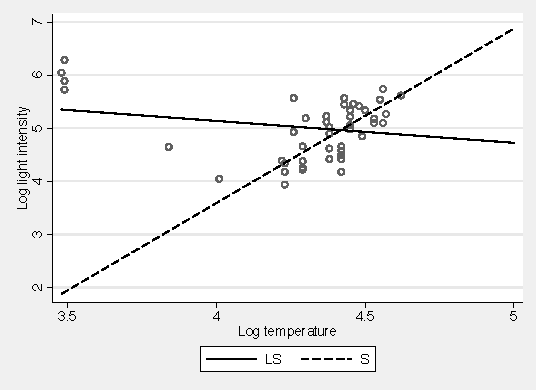
\epsfig{file=eps/4/4}
    \caption{\alert{Caption needed}}
    \label{fig:stars_scatterplot}
\end{figure}

To obtain the \stsc{LS} estimates for the intercept and slope of the regression
of log intensity on log temperature in Stata, without making any difference 
between stars, we can type:

\begin{stlog}
. use Star.dta, clear
{\smallskip}
. regress log_intensity log_temperature
{\smallskip}
      Source {\VBAR}       SS           df       MS      Number of obs   =        47
\HLI{13}{\PLUS}\HLI{34}   F(1, 45)        =      2.08
       Model {\VBAR}  .664593334         1  .664593334   Prob > F        =    0.1557
    Residual {\VBAR}  14.3463934        45  .318808743   R-squared       =    0.0443
\HLI{13}{\PLUS}\HLI{34}   Adj R-squared   =    0.0230
       Total {\VBAR}  15.0109868        46  .326325799   Root MSE        =    .56463
{\smallskip}
\HLI{14}{\TOPT}\HLI{64}
log_intensity {\VBAR}      Coef.   Std. Err.      t    P>|t|     [95\% Conf. Interval]
\HLI{14}{\PLUS}\HLI{64}
log_tempera{\tytilde}e {\VBAR}  -.4133041   .2862575    -1.44   0.156    -.9898562     .163248
        _cons {\VBAR}   6.793468   1.236516     5.49   0.000     4.302998    9.283939
\HLI{14}{\BOTT}\HLI{64}
{\smallskip}

\end{stlog}

The results of the \stsc{LS} estimation (solid line in
figure~\ref{fig:stars_scatterplot}) indicate that, against intuition, if the
temperature of a star increases, its light intensity decreases in average
(although the effect is not significantly different from zero). If instead of
using a classical estimator we use a robust estimator, the result changes
drastically. For illustrative purposes we will estimate the above model using
\stsc{LTS}, \stsc{LMS}, \stsc{M}, \stsc{GM}, \stsc{S} and \stsc{MM} (with an
efficiency fixed at 95\%) estimators. However, since it has now been widely
accepted that \stsc{S} and \stsc{MM} estimators are preferable to LTS and LMS
because of their higher efficiency and to \stsc{M} and \stsc{GM} estimator
because of their higher robustness with respect to outliers (see above), in the
subsequent examples we will focus exclusively on \stsc{S} and \stsc{MM}
estimates.

\paragraph{LTS}

A robust \stsc{LTS} estimator can be easily fit using the \stcmd{robreg} package 
running the following command:

\begin{stlog}
. robreg lts log_light log_temp
{\smallskip}
enumerating 500 samples (percent completed)
0 \HLI{5} 20 \HLI{6} 40 \HLI{6} 60 \HLI{6} 80 \HLI{5} 100
..................................................
{\smallskip}
LTS regression                                  Number of obs     =         47
                                                  Breakdown point =         .5
                                                  Subsamples      =        500
                                                  Scale estimate  =  .40961741
{\smallskip}
\HLI{13}{\TOPT}\HLI{64}
   log_light {\VBAR}      Coef.
\HLI{13}{\PLUS}\HLI{64}
    log_temp {\VBAR}   4.727267
       _cons {\VBAR}  -15.81634
\HLI{13}{\BOTT}\HLI{64}
{\smallskip}

\end{stlog}

The results from the \stsc{LTS} estimator are
very different from those obtained for the \stsc{LS} estimation. Indeed what we
observe here is that if the log of the temperature of a star increases, its
luminosity will increase as well. In term of size of effect, the \stsc{LTS} estimator
suggests that an increase of 100\% of the temperature is associated to an
increase of the luminosity of approximately 473\%.

\paragraph{LMS}

If instead of the \stsc{LTS} estimator we wish to use the \stsc{LMS} estimator,
we can type:

\begin{stlog}
. robreg lms log_light log_temp
{\smallskip}
enumerating 500 samples (percent completed)
0 \HLI{5} 20 \HLI{6} 40 \HLI{6} 60 \HLI{6} 80 \HLI{5} 100
..................................................
{\smallskip}
LMS regression                                  Number of obs     =         47
                                                  Subsamples      =        500
                                                  Scale estimate  =  .36429398
{\smallskip}
\HLI{13}{\TOPT}\HLI{64}
   log_light {\VBAR}      Coef.
\HLI{13}{\PLUS}\HLI{64}
    log_temp {\VBAR}   3.636368
       _cons {\VBAR}  -11.20184
\HLI{13}{\BOTT}\HLI{64}
{\smallskip}

\end{stlog}

Even if the size of effect seems to be slightly smaller than with \stsc{LTS},
the sign of the relation is the same pointing towards a positive association
between log-temperature and lightness of stars.

\paragraph{M-estimator}

If we use the \stsc{M} estimator (with a Huber
loss function), we do not expect the estimation to resist to outliers. Indeed, 
in the theoretical section it has been shown how this
estimator resists to vertical outliers but not to bad leverage points (i.e.
points outlying in the space of the explanatory variables). As expected, the
\stsc{M} estimation provides results very similar to those of \stsc{LS} and we can conclude
that the estimator breaks down.

The command to run the \stsc{M} estimator is:

\begin{stlog}
. robreg m log_intensity log_temperature
fitting initial LAV estimate ... done
iterating RWLS estimate ........... done
{\smallskip}
M-Regression (95\% efficiency)                   Number of obs     =         47
                                                  Huber k         =  1.3449986
                                                  Scale estimate  =  .63061122
                                                  Robust R2 (w)   =  .04761698
                                                  Robust R2 (rho) =  .03486282
{\smallskip}
\HLI{14}{\TOPT}\HLI{64}
              {\VBAR}               Robust
log_intensity {\VBAR}      Coef.   Std. Err.      z    P>|z|     [95\% Conf. Interval]
\HLI{14}{\PLUS}\HLI{64}
log_tempera{\tytilde}e {\VBAR}  -.4235066   .3992983    -1.06   0.289    -1.206117    .3591036
        _cons {\VBAR}    6.84754   1.758148     3.89   0.000     3.401634    10.29345
\HLI{14}{\BOTT}\HLI{64}
{\smallskip}

\end{stlog}

\paragraph{GM-estimator}

The Generalized \stsc{M} estimate is slightly more complicated to compute than
the \stsc{M} estimate. We first need to estimate the outlyingness of each
individual in the x-dimension, and then downweight leverage points while
estimating the model using an \stsc{M} estimator. In this example, given that
there is a single explanatory variable, the outlyingness in the horizontal
dimension can be measured by centering the data around a robustly estimated
location parameter (e.g. the Hodges-Lehman estimate or the median) and reducing
it using a robustly estimated measure of dispersion (e.g. the Croux and
Rousseeuw $Q_{n}$ estimate). In the case of multiple explanatory variables, the
outlyingness in the space of the explanatory variables will have to be measured
using robust multivariate estimates of location and scatter described in
chapter \alert{XXX}. As far as the down-weighting scheme for outliers is
concerned, several alternatives have been proposed in the literature. In this
example we award a weight equal to zero to any star associated to a leverage
larger than 2.5 and equal to one otherwise. Given that there is one single
explanatory variable, the \stsc{GM} estimator should behave satisfactory.

The commands used for \stsc{GM} estimation are:                                 \todo{To be updated}

\begin{stlog}
. robstat log_temp, statistics(hl qn)
{\smallskip}
Robust Statistics                 Number of obs   =         47
{\smallskip}
\HLI{13}{\TOPT}\HLI{48}
    log_temp {\VBAR}      Coef.   Std. Err.     [95\% Conf. Interval]
\HLI{13}{\PLUS}\HLI{48}
          HL {\VBAR}      4.375          .             .           .
          Qn {\VBAR}   .1553394   .0235479      .1079401    .2027388
\HLI{13}{\BOTT}\HLI{48}
{\smallskip}
. generate leverage = (log_temp - _b[HL])/_b[Qn]
{\smallskip}
. robreg m log_light log_temp if abs(leverage)<=2.5
fitting initial LAV estimate ... done
iterating RWLS estimate ..... done
{\smallskip}
M-Regression (95\% efficiency)                   Number of obs     =         42
                                                  Huber k         =  1.3449986
                                                  Scale estimate  =  .45145187
                                                  Robust R2 (w)   =  .50939875
                                                  Robust R2 (rho) =   .4685587
{\smallskip}
\HLI{13}{\TOPT}\HLI{64}
             {\VBAR}               Robust
   log_light {\VBAR}      Coef.   Std. Err.      z    P>|z|     [95\% Conf. Interval]
\HLI{13}{\PLUS}\HLI{64}
    log_temp {\VBAR}   2.908649   .3751616     7.75   0.000     2.173346    3.643952
       _cons {\VBAR}  -7.875076   1.664063    -4.73   0.000    -11.13658   -4.613572
\HLI{13}{\BOTT}\HLI{64}
{\smallskip}
. drop leverage
{\smallskip}

\end{stlog}


\paragraph{S-estimator}

If we estimate the model using an \stsc{S} estimator, we do not expect to have
large differences with respect to \stsc{LTS}, \stsc{LMS} and \stsc{GM} in terms
of point estimates. However, its higher efficiency makes it theoretically more
appealing. The command to run the \stsc{S} estimator is:

\begin{stlog}
. robreg s log_intensity log_temperature
{\smallskip}
enumerating 50 candidates (percent completed)
0 \HLI{5} 20 \HLI{6} 40 \HLI{6} 60 \HLI{6} 80 \HLI{5} 100
..................................................
{\smallskip}
refining 2 best candidates ... done
{\smallskip}
S-Regression (28.7\% efficiency)                 Number of obs     =         47
                                                  Subsamples      =         50
                                                  Breakdown point =         .5
                                                  Bisquare k      =   1.547645
                                                  Scale estimate  =  .47145696
{\smallskip}
\HLI{14}{\TOPT}\HLI{64}
              {\VBAR}               Robust
log_intensity {\VBAR}      Coef.   Std. Err.      z    P>|z|     [95\% Conf. Interval]
\HLI{14}{\PLUS}\HLI{64}
log_tempera{\tytilde}e {\VBAR}   3.290339    1.64075     2.01   0.045     .0745278    6.506151
        _cons {\VBAR}  -9.570732   7.373867    -1.30   0.194    -24.02325    4.881783
\HLI{14}{\BOTT}\HLI{64}
{\smallskip}

\end{stlog}

The results indicate that if the temperature of a star doubles, its light
intensity increases by approximately 329\%. As stated in the theoretical
section, the gaussian efficiency of the \stsc{S} estimator with a 50\%
breakdown point (and a Tukey biweight loss function) is only 28\%. In order to
increase the efficiency while keeping the breakdown point at 50\%, we can use
\stsc{MM} estimators.

\paragraph{\stsc{MM} estimator}

It is well-known that even if an \stsc{MM} estimator has a breakdown point of 50\%,
it can be associated to a relatively large bias if its efficiency is set too
high. As explained in Subsection \ref{subsec:Hausman}, a general procedure is
therefore to compare the \stsc{MM} estimate with a given level of efficiency to the
S-estimate, and see if there is a significant difference. If the difference
is small, this means that the bias should not be too big.

We compute here an \stsc{MM} estimator with an efficiency set at 95\%:


\begin{stlog}
. robreg mm log_intensity log_temperature, efficiency(95)
{\smallskip}
Step 1: fitting S-estimate
{\smallskip}
enumerating 50 candidates (percent completed)
0 \HLI{5} 20 \HLI{6} 40 \HLI{6} 60 \HLI{6} 80 \HLI{5} 100
..................................................
{\smallskip}
refining 2 best candidates ... done
{\smallskip}
Step 2: fitting redescending M-estimate
{\smallskip}
iterating RWLS estimate .............. done
{\smallskip}
MM-Regression (95\% efficiency)                  Number of obs     =         47
                                                  Subsamples      =         50
                                                  Breakdown point =         .5
                                                  M-estimate: k   =   4.685045
                                                  S-estimate: k   =   1.547645
                                                  Scale estimate  =  .47145688
                                                  Robust R2 (w)   =  .41883093
                                                  Robust R2 (rho) =  .02050865
{\smallskip}
\HLI{14}{\TOPT}\HLI{64}
              {\VBAR}               Robust
log_intensity {\VBAR}      Coef.   Std. Err.      z    P>|z|     [95\% Conf. Interval]
\HLI{14}{\PLUS}\HLI{64}
log_tempera{\tytilde}e {\VBAR}   2.253165   .7690643     2.93   0.003     .7458263    3.760503
        _cons {\VBAR}  -4.969402   3.410051    -1.46   0.145    -11.65298    1.714175
\HLI{14}{\BOTT}\HLI{64}
{\smallskip}

\end{stlog}

We see that the \stsc{MM} estimation leads to results comparable to the
\stsc{S} estimation in terms of point estimates but is associated to a much
higher efficiency. As explained above, a formal test could have been used but
we leave this for another example. The \stsc{MM} estimated model suggests that
an increase of 100\% of the temperature of a star is associated with an
increase of its luminosity by approximately 225\%. In terms of the quality of
the fit, if we rely on the robust $R^2(w)$ described previously, we see that
the model is pretty good in predicting the luminosity of stars for the vast
majority of the observations. Indeed close to 42\% of the variations in terms
of light intensity for the vast majority of the observations can be explained
by the differences in temperatures.


\subsubsection{Identifying outliers} 

In this second example where the objective is
to unmask outliers, we use a dataset made available by Jeffrey D. Sachs and
Andrew M. Warner in their article \textquotedblleft Natural Resource Abundance
and Economic Growth\textquotedblright\ (1997). In this paper, the authors show
that economies with a high ratio of natural resource exports to GDP in 1970
(the base year) tended to grow slowly during the subsequent 20-year period
1970-1990. In the article the authors aknowledge the existence of outliers and
try to deal with them working with differences in fits.\ More precisely, they
look at how the predicted value for each observation varies when this specific
observation is removed from the sample when fitting the model and compare the
results with the model estimated using all of the observations. They expect to
see big differences in fits for outlying individuals.\ However, if there are
clusters of outliers, atypical individuals will mask one the other and will
most probably not be detected with this technique. The outliers they identify
are Chad, Gabon, Guyana, and Malaysia.

We propose here to use another procedure to identify the outliers. This
procedure is simply based on the examination of the standardized residuals
related to a regression S-estimator.

To identify the outliers, we fist estimate the regression model by running the
command :%

%TCIMACRO{\TeXButton{TeX field}{\tt}}%
%BeginExpansion
%\tt
%EndExpansion
\texttt{robreg s gea7090 lgdpea70 sxp sopen linv7089 rl dtt7090}%
%TCIMACRO{\TeXButton{TeX field}{\it}}%
%BeginExpansion
%\it
%EndExpansion


The results of this S-estimation are presented in Figure ?.%\ref{fig:countries_S_results}.

\textbf{[Insert here S graph from Ch3-Ex-2.do]} \ \newline\ We ask for
the predicted values of the dependent variable by the command:
%TCIMACRO{\TeXButton{TeX field}{\tt}}%
%BeginExpansion
%\tt
%EndExpansion
\texttt{predict yhat}%
%TCIMACRO{\TeXButton{TeX field}{\it}}%
%BeginExpansion
%\it
%EndExpansion
. The robust residuals can then be easily determined using the command:
%TCIMACRO{\TeXButton{TeX field}{\tt}}%
%BeginExpansion
%\tt
%EndExpansion
\texttt{gen res=yhat-gea7090}%
%TCIMACRO{\TeXButton{TeX field}{\it}}%
%BeginExpansion
%\it
%EndExpansion
. They are standardized by dividing them by the scale parameter estimated from
the regression S-estimate:%
%TCIMACRO{\TeXButton{TeX field}{\tt}}%
%BeginExpansion
%\tt
%EndExpansion
\texttt{replace res=res/e(scale)}%
%TCIMACRO{\TeXButton{TeX field}{\it}}%
%BeginExpansion
%\it
%EndExpansion
. We can now plot the standardized residuals and identify those that are
larger or smaller than two given cut-off points corresponding to two specific
quantiles of the normal distribution. We use here the percentiles 2.5 and 97.5
which are respectively equal to -1.96 and 1.96.

We see in Figure ?%\ref{fig:countries_S_standardized_res} 
that, among the four
countries identified as outliers by Sachs and Warner, only Malaysia is still
emerging as outlier when using the S-estimation procedure. On the other hand,
other countries such as Hong Kong, Ecuador or Iran seem to be atypical
countries in the S-regression but were not detected by the original authors.



\textbf{[Insert here S graph from Ch3-Ex-2.do]} \ \newline

\begin{stexample}
\textbf{Testing for the presence of outliers and setting the efficiency for
MM-estimation. }For this example, we again use the dataset relating the
logarithm of the effective temperature at the surface of the star (explanatory
variable $T_{e}$) and the logarithm of its light intensity (dependent variable
$L/L_{0}$). The first question one might raise is: is there a significant
difference between the classical estimate and the robust one? To answer this
question we simply compute an S-estimate using the
%TCIMACRO{\TeXButton{TeX field}{\tt}}%
%BeginExpansion
%\tt
%EndExpansion
\texttt{robreg s}%
%TCIMACRO{\TeXButton{TeX field}{\it} }%
%BeginExpansion
%\it
%EndExpansion
command and use
%TCIMACRO{\TeXButton{TeX field}{\tt}}%
%BeginExpansion
%\tt
%EndExpansion
\texttt{hausman}%
%TCIMACRO{\TeXButton{TeX field}{\it} }%
%BeginExpansion
%\it
%EndExpansion
as an option. This implies that the testing procedure comparing the S-estimate
with the \stsc{LS} estimate (see Subsection \ref{subsec:Hausman}) is implemented.

\textbf{[Insert here S regression from Ch3-Ex-3.do]} \ \newline

The results of the Hausman test (see Figure ?%\ref{fig:stars_Hausman_SvsLS}
)
clearly indicate that the difference between the S-estimate and the
LS-estimate is significant (p-value%
%TCIMACRO{\TEXTsymbol{<}}%
%BeginExpansion
$<$%
%EndExpansion
0.05) and thus that outliers distort the \stsc{LS} estimation. We should therefore
use a robust estimator.

As stated previously S-estimators are very robust against outlier
contamination but are relatively inefficient. \stsc{MM} estimators on the other hand
are more efficient than S-estimators but might be associated with a large bias
if efficiency is set too high. To choose the level of efficiency to use in
practice we have to apply the testing procedure described in Subsection
\ref{subsec:Hausman} that compares the MM-estimates related to some given
levels of efficiency with respect to an S-estimate. We can then finally set
the efficiency of the \stsc{MM} estimator at the highest efficiency level that does
not lead to a rejection of the equality between the MM-estimate and the
S-estimate. Doing this in practice is very simple as the testing procedure is
implemented in the
%TCIMACRO{\TeXButton{TeX field}{\tt}}%
%BeginExpansion
%\tt
%EndExpansion
\texttt{robreg mm}%
%TCIMACRO{\TeXButton{TeX field}{\it} }%
%BeginExpansion
%\it
%EndExpansion
command.\ For example, if the
%TCIMACRO{\TeXButton{TeX field}{\tt}}%
%BeginExpansion
%\tt
%EndExpansion
\texttt{robreg mm}%
%TCIMACRO{\TeXButton{TeX field}{\it}}%
%BeginExpansion
%\it
%EndExpansion
\texttt{ }command is run with the efficiency set at 75\% , the
%TCIMACRO{\TeXButton{TeX field}{\tt}}%
%BeginExpansion
%\tt
%EndExpansion
\texttt{hausman}%
%TCIMACRO{\TeXButton{TeX field}{\it} }%
%BeginExpansion
%\it
%EndExpansion
option compares the MM-estimate with 75\% efficiency to the S-estimate
obtained at the first step of the MM-estimation procedure. Similarly, if the
efficiency is set at 85\%, the
%TCIMACRO{\TeXButton{TeX field}{\tt}}%
%BeginExpansion
%\tt
%EndExpansion
\texttt{hausman}%
%TCIMACRO{\TeXButton{TeX field}{\it} }%
%BeginExpansion
%\it
%EndExpansion
option compares the MM-estimate with 85\% efficiency to the S-estimate, and so
on. In this example we control if we can set the efficiency at 75\%, 85\%,
95\%, and 99\%. We obtain the following results:

\begin{itemize}
\item \textbf{MM-estimation with 75\% efficiency:}%

%TCIMACRO{\TeXButton{TeX field}{\tt}}%
%BeginExpansion
%\tt
%EndExpansion
\texttt{robreg mm log\_intensity log\_temperature, hausman efficiency(75)}%
%TCIMACRO{\TeXButton{TeX field}{\it}}%
%BeginExpansion
%\it
%EndExpansion


\textbf{[Insert here MM(75) regression from Ch3-Ex-3.do]} \ \newline

The results of the Hausman test (see Figure ?%\ref{fig:stars_Hausman_SvsMM75}
)
indicate that there is no significant difference between the MM-estimate and
the S-estimate. It would therefore be preferable to work with the \stsc{MM} estimator
with an efficiency equal to 75\% as it provides results comparable to the
S-estimator in terms of bias but has a much higher efficiency.

\item \textbf{MM-estimation with 85\% efficiency:}%

%TCIMACRO{\TeXButton{TeX field}{\tt}}%
%BeginExpansion
%\tt
%EndExpansion
\texttt{robreg mm log\_intensity log\_temperature, hausman efficiency(85)}%
%TCIMACRO{\TeXButton{TeX field}{\it}}%
%BeginExpansion
%\it
%EndExpansion


\textbf{[Insert here MM(85) regression from Ch3-Ex-3.do]} 

Here again the Hausman test statistics takes a low value which tells us that
there is no significant difference between the MM-estimate and the S-estimate.

\item \textbf{MM-estimation with 95\% efficiency:}%

%TCIMACRO{\TeXButton{TeX field}{\tt}}%
%BeginExpansion
%\tt
%EndExpansion
\texttt{robreg mm log\_intensity log\_temperature, hausman efficiency(95)}%
%TCIMACRO{\TeXButton{TeX field}{\it}}%
%BeginExpansion
%\it
%EndExpansion


\textbf{[Insert here MM(95) regression from Ch3-Ex-3.do]} 

If we set the efficiency of the \stsc{MM} estimator to 95\%, we still do not observe
any significant difference between the MM-estimate and the S-estimate.

\item \textbf{MM-estimation with 99\% efficieny:}%

%TCIMACRO{\TeXButton{TeX field}{\tt}}%
%BeginExpansion
%\tt
%EndExpansion
\texttt{robreg mm log\_intensity log\_temperature, hausman efficiency(99)}%
%TCIMACRO{\TeXButton{TeX field}{\it}}%
%BeginExpansion
%\it
%EndExpansion


\textbf{[Insert here MM(99) regression from Ch3-Ex-3.do]} 

In the case of an efficiency of the \stsc{MM} estimator equal to 99\%, the Hausman
test rejects the null hypothesis of equality between the MM-estimate and the
S-estimate, which means that for this very high level of efficiency, the
\stsc{MM} estimator suffers from a too large bias.

To summarize, it is clear that a classical estimator cannot be used in the
example because the \stsc{LS} estimates are clearly distorted. A robust estimator
should be prefered. We may use an \stsc{MM} estimator with an efficiency equal to
95\% instead of the less efficient S-estimator since despite the bias from
which the \stsc{MM} estimator potentially suffers, the MM-estimates of the regression
parameters appear no significantly different from the S-estimates. It is not
recommended to consider a higher level of efficiency for the \stsc{MM} estimator
(99\%, for instance), since the statistical test indicates that the bias
becomes too big in that case.
\end{itemize}
\end{stexample}

\begin{stexample}
\textbf{Recognizing the type of outliers} For this example, we will use the
very famous auto dataset available from Stata. This dataset contains the price
of a set of cars as well as a series of characteristics. To see if outliers
are present in the dataset, we regress the price on all the available
characteristics and compute the robust standardized residuals. Obviously this
will not allow to recognize the types of outliers. To do so, we will use the
graphical tool of Rousseuw and Van Zomeren (1990).\ The idea here is to use a
scatter plot considering on the vertical dimension the standardized residuals
and on the horizontal dimension the leverage of the observations measured
using the robust Mahalanobis distance (as described in (\ref{eq:leverage})).
For gaussian data it is well known that the standardized residuals are
normally distributed while the robust distances are distributed as a $\chi
_{p}^{2}$ where $p$ is the number of continuous explanatory variables. It is
then natural to compare the standardized residuals and the leverages to some
specific quantiles of the $\mathcal{N}(0,1)$ or $\chi_{p}^{2}$ distributions
in order to detect if an individual has to be considered as an outlier and, if
it is the case, to which type of outlier it corresponds. We decide to choose
here the 2.5th and 97.5th percentiles of the $\mathcal{N}(0,1)$ distribution,
and the 95th percentile of the $\chi_{p}^{2}$ distribution. Those individuals
leading to small robust standardized residuals in absolute value and small
leverages are considered as standard individuals; those giving large
standardized residuals in absolute value and large leverages are defined as
bad leverage points; those that coincide with large standardized residuals in
absolute value but small leverages are considered as vertical outliers and,
finally, those that give small standardized residuals in absolute value but
large leverages are good leverage points. \newline

\textbf{[Insert here MM(95)
regression from Ch3-Ex-4.do]}  \newline\textbf{[Insert here MM(95) graphn from
Ch3-Ex-4.do]}\newline 

Figure ?%\ref{fig:autos_res_leverages} 
clearly shows, for
example, that the Cadillac Seville is a bad leverage point.\ This auto is
indeed associated with a very large positive robust standardized residual and
has a big leverage effect which means that its characteristics in the space of
the explanatory variables are very different from the bulk of the data. On the
other hand, the Cadillac Eldorado, the Lincoln Versaille and some other cars
have a small leverage effect --- their characteristics do not appear as
different from the vast majority of the observations --- but are highly
overpriced given their large positive residuals; these cars are identified as
vertical outliers. Finally some other cars such as the Plymouth Arrow or the
Volkswagen (VW Diesel) \emph{inter alia} are not outliers in terms of prices
but have characteristics very different from the others.\ They are thus good
leverage points. Note that even if these good leverage points do not have
major effect on the estimation of the slope parameter and the constant, they
might affect inference and shrink standard errors.\ It is hence important for
researchers to identify them.
\end{stexample}


\begin{stexample}
\textbf{Dealing with dummies}. For this example, we use the "fertil1.dta" data
set provided provided by Wooldridge (2001) which is a pooled cross section on
more than a thousand U.S. women for the even years between 1972 and 1984.
These data are used to study the relationship between women's education and
fertility. We estimate a model relating the number of children ever born to a
woman (kids) to the years of education, age, age squared, regional dummies,
race dummies, the type of environment in which the women have been reared and
year dummies, using an MS-estimator.\ Given the large number of dummy
variables, it is very likely that the subsampling algorithm described in
Subsection \ref{subsec:MM_estimation} leads to perfectly collinear subsamples.
Using an MS-estimator should tackle the problem.\newline

\textbf{[Insert here MS regression from Ch3-Ex-5.do]}\newline

The results presented in Figure fig:fertil1\_MS\_results clearly point towards
a robust and statistically significant negative relationship between education
and fertility.\ Indeed, each additionnal year of schooling is associated to an
average reduction of fertility (i.e. number of children) equal to 0.19. To
identify the outliers and recognize their type, we again call on the graphical
tool proposed by Rousseuw and Van Zomeren (1990).\ The only difference with
the previous example is that dummy explanatory variables cannot create any
leverage effect and should therefore be treated \ differently from the other
explanatory variables.\ To estimate robust distances, we rely on the Stahel
and Donoho multivariate estimator of location and scatter (this estimator will
be described in details in Chapter ??).\ The latter is a projection based
estimator that allows the pratialling out of dummy variables to calculate
leverage effects. As before we can choose a quantile above which individuals
can be seen as potentially outlying.\ We use here the 0.5th and 99.5th
percentiles of the $\mathcal{N}(0,1)$ distribution as cut-off points for the
robust standardized residuals, and the 99th percentile\ of the chi-square
distribution with $p_{1}$ degrees of freedom, where $p_{1}$ is the number of
continuous explanatory variables, as cut-off point for the robust distances.
In Figure %\ref{fig:fertil1_res_leverages}
, we highlight the women for which
the robust standardized residuals and (or) the robust distances exceed the
cut-off points.

\textbf{[Insert here  graphn from Ch3-Ex-5.do]}\newline

It is evident that individuals such as 565 have more children that one would
expect given their characteristics (which are not quite\textbf{ }different
from the bulk of the data). On the other hand individuals such as 706, 767 or
1063 have characteristics that are very different from the vast majority of
the individuals; however their number of children is in accordance with her
characteristics. Finally individual such as 519, or 490 or 967 have
characteristics that are very different from the others.\ The first one has a
number of children that is much smaller than one would expect according to the
estimated model while the two others have more children than expected.
\end{stexample}

\section{Appendix 1: M-estimators of location and scale}
\label{sec:robreg:appendix1}

The application of the M-estimation approach in the particular case of the
location-scale model (\ref{eq:location_scale_model}) leads to the M-estimators
of location and scale.

\subsection{M-estimator of location}

An M-estimate $\sthat{\mu}_{\stsc{M};\rho}$ of $\mu$ is defined by%

\[
\sthat{\mu}_{\stsc{M};\rho}=\argmin_{\mu}\sum_{i=1}^{n}\rho\left(
\frac{y_{i}-\mu}{\sthat{\sigma}}\right)
\]
where $\rho\left(  \cdot\right)  $ is a loss function that is positive, even
(such that $\rho\left(  0\right)  =0$) and not decreasing for positive values
$u$, and $\sthat{\sigma}$ is a preliminary robust estimate of $\sigma$ if
this scale parameter is unknown (the MAD, for example). We may also
characterize $\sthat{\mu}_{\stsc{M};\rho}$ as a solution of the following
estimating equation:
\begin{equation}
\sum_{i=1}^{n}\psi\left(  \frac{y_{i}-\mu}{\sthat{\sigma}}\right)  =0,
\label{eq:M_location_equation}%
\end{equation}
where $\psi(u)=\rho^{\prime}(u)$.

Taking $\rho\left(  u\right)  =u^{2}$, we obtain $\psi\left(  u\right)  =2u$
and hence
\[
\sum_{i=1}^{n}\left(  y_{i}-\sthat{\mu}_{\stsc{M};\rho}\right)  =0,
\]
implying that $\sthat{\mu}_{\stsc{M};\rho}=\frac{1}{n}\sum_{i=1}^{n}%
y_{i}=\sthat{\mu}_{\stsc{LS}}$. Taking $\rho\left(  u\right)  =\left\vert
u\right\vert $, we have $\psi(u)=\mathrm{sgn}(u)$ and $\sum_{i=1}%
^{n}\mathrm{sgn}\left(  y_{i}-\sthat{\mu}_{\stsc{M};\rho}\right)  =0$;
this leads to $\sthat{\mu}_{\stsc{M};\rho}=\mathrm{med}\left\{
y_{i}\right\}  =\sthat{\mu}_{\mathrm{L}_{\mathrm{1}}}$.

In general, if $\psi$ is not redescending, the equation
(\ref{eq:M_location_equation}) may be solved using the Newton-Raphson
algorithm with a robust estimate of $\mu$ --- the empirical median
$\mathrm{med}\left\{  y_{i}\right\}  $, for instance --- as initial value for
$\mu$.

The influence function of the functional $T$ associated to the location
M-estimator $\sthat{\mu}_{\stsc{M};\rho}$ under the distribution $F_{0,1}$
of the error term $\nu$ in the location-scale model \ --- recall here that
$F_{0,1}$ is assumed to be symmetric around zero --- takes the form:
\[
\mathrm{IF}\left(  u;T,F_{0,1}\right)  =\frac{\psi(u)}{\mathrm{E}_{F_{0,1}%
}\left[  \psi^{\prime}\left(  \nu\right)  \right]  }.
\]
Consequently, the choice of the function $\rho$, and hence of the function
$\psi$, completely conditions the form of the influence function.

Moreover, it has been proven that an univariate location M-estimator has an
asymptotic breakdown point equal to 50\% whenever the function $\psi$ is
\emph{non decreasing}, bounded and symmetric, and the preliminary estimator of
the scale parameter $\sigma$ is the MAD\footnote{The breakdown point of
$\sthat{\boldsymbol\beta}_{\stsc{M};\rho}$ is actually equal to the
breakdown point of the preliminary estimator of the scale parameter $\sigma$.}
(see \citealp[54]{Huber:2009}). The asymptotic breakdown point is
nul if $\psi$ is unbounded. If $\psi$ is equal to the function $\psi_{\kappa
}^{\stsc{B}}$ and hence is redescending, the breakdown point of
$\sthat{\mu}_{\stsc{M};\rho}$ is strictly smaller than 50\% and depends
upon the breakdown point of the preliminary scale estimator, upon the constant
$\kappa$, but also upon the configuration of the sample (see
\citealp[78]{maronna:etal:2006})\footnote{Note however that it is
possible to prove that, using the MAD as initial scale estimator, the
breakdown point of $\sthat{\mu}_{\stsc{M};\rho_{\kappa}^{\stsc{B}}}$ is
strictly greater than 0.49 in the Gaussian case.}.

\subsection{M-estimator of scale}

A M-estimate $\sthat{\sigma}_{\stsc{M};\rho}$ of the scale parameter
$\sigma$ is defined as the solution of the equation
\begin{equation}
\frac{1}{n}\sum_{i=1}^{n}\rho\left(  \frac{y_{i}-\sthat{\mu}}{\sigma
}\right)  =\delta\label{eq:M_scale_loc_equation}%
\end{equation}
where $\rho\left(  \cdot\right)  $ is a loss function that is positive, even,
not decreasing for positive values and bounded, and $\sthat{\mu}$ is a
preliminary robust estimate of $\mu$ if this location parameter is unknown
(the median, for instance). To ensure the consistency of $\sthat{\sigma
}_{\stsc{M};\rho}$ for $\sigma$, we have to take $\delta=\mathrm{E}%
_{F_{0,1}}\left[  \rho\left(  \nu\right)  \right]  $. An usual choice for the
loss function $\rho$ is the Tukey-Biweight function $\rho_{\kappa}^{B}$
defined by (\ref{eq:Tukey_Biweight_function}).

The M-estimators of scale are translation invariant and scale equivariant. The
influence function of the functional $S$ associated to the scale M-estimator
$\sthat{\sigma}_{\stsc{M};\rho}$ under the distribution $F_{0,1}$ of the
error term $\nu$ of the location-scale model is given by
\[
\mathrm{IF}\left(  u;S,F_{0,1}\right)  =\frac{\rho\left(  u\right)  -\delta
}{\mathrm{E}_{F_{0,1}}\left[  \rho^{\prime}\left(  \nu\right)  \nu\right]  }.
\]
Hence, the choice of a bounded function $\rho$ implies that the influence
function is also bounded. The asymptotic breakdown point of the scale
M-estimator is:
\[
\varepsilon^*\left(  S,F_{0,1}\right)  =\min\left(  \frac{\delta}%
{\rho\left(  \infty\right)  },1-\frac{\delta}{\rho\left(  \infty\right)
}\right)  ,
\]
which is strictly positive but not always equal to 50\%, even if $\rho$ is bounded.

\begin{stremark}
We may try to jointly estimate $\mu$ and $\sigma$ by solving simultaneously
two equations of the type (\ref{eq:M_location_equation}) and
(\ref{eq:M_scale_loc_equation}) (see, for example, \citealp{Huber:2009}, chapter 6). This complexifies the computations. Moreover, as
explained in \cite{maronna:etal:2006}, it generally provides for
$\sthat{\mu}_{\stsc{M};\rho}$ an asymptotic breakdown point smaller than
50\% --- hence, smaller than the breakdown point attainable by using the MAD
as preliminary estimator of $\sigma$. Consequently, the joint estimation of
$\mu$ and $\sigma$ is not recommended, especially when the scale parameter
$\sigma$ is considered as a nuisance parameter in the location-scale model.
\end{stremark}

\section{Appendix 2: Generalized Method of Moments (GMM) and asymptotic distributions of regression M, S and MM estimators}
\label{sec:robreg:appendix2}

\subsection{GMM-estimation principle}

For simplicity, let us consider immediately the context of the regression
model (\ref{eq:linear_regr_model}). Let $y$ be the scalar dependent variable
and $\stvec{x}=\left(  1,x_{1},\ldots,x_{p}\right)  ^{t}$ be the $\left(
p+1\right)  $-vector of covariates. We assume here that the observations
$\left(  \stvec{x}_{1},y_{1}\right)  ,\ldots,\left(  \stvec{x}_{n}%
,y_{n}\right)  $ are generated by a \emph{stationary}\footnote{A
\emph{stationary} process is a stochastic process whose joint probability
distribution does not change when shifted in time or space. Consequently,
parameters such as the mean and the variance, if they exist, also do not
change over time or position . Hence, the mean and the variance of the process
do not follow trends.} and \emph{ergodic}\footnote{A stochastic process is
said to be \emph{ergodic} if its statistical properties (such as its mean
and variance) can be estimated consistently from a single, sufficiently long
sample (realization) of the process.} process $H$. We also assume, to avoid
too much technicalities, that there is \emph{no autocorrelation}, that is,
that the observations $\left(  \stvec{x}_{i},y_{i}\right)  $, $i = 1, \dots, n$,
are \emph{independent}.\footnote{The interested reader can find very general
results, valid in presence of autocorrelation, in
\cite{Croux:2003}.}

Suppose that our objective is to estimate the functional $\boldsymbol{\theta
}=\boldsymbol{\theta}\left(  H\right)  $ that is implicitly defined by the
equation
\begin{equation}
\mathrm{E}_{H}\left[  \mathbf{m}\left(  y,\stvec{x},\boldsymbol{\theta
}\right)  \right]  =\stvec{0}, \label{Eq:GMM_moments_conditions}%
\end{equation}
where $\mathbf{m}$ is a known $k$-valued function, and $\mathrm{E}_{H}\left[
\cdot\right]  $ denotes the mathematical expectation with respect to $H$. If
$k$ equals the dimension of the parameter $\boldsymbol{\theta}$ to estimate,
i.e., if the number of moments conditions specified by
(\ref{Eq:GMM_moments_conditions}) co\"{\i}ncides with the dimension of
$\boldsymbol{\theta}$, then the GMM estimation problem is said to be
\emph{exactly-identified}. Note that it is the case in the setting studied
hereafter. The GMM estimator $\sthat{\boldsymbol{\theta}}_{\mathrm{GMM}}$ of
$\boldsymbol{\theta}$ is then simply obtained by solving the sample analogue
of (\ref{Eq:GMM_moments_conditions}), that is,
\begin{equation}
\frac{1}{n}\sum_{i=1}^{n}\mathbf{m}\left(  y_{i},\stvec{x}_{i},\widehat
{\boldsymbol{\theta}}_{\mathrm{GMM}}\right)  =\stvec{0}.
\label{Eq:GMM_equations}%
\end{equation}


Under regularity conditions detailed in \citet{Hansen:1982}, the GMM
estimator $\sthat{\boldsymbol{\theta}}_{\mathrm{GMM}}$ defined by
(\ref{Eq:GMM_equations}) has a limiting normal distribution: \
\begin{equation}
\sqrt{n}\left(  \sthat{\boldsymbol{\theta}}_{\mathrm{GMM}}%
-\boldsymbol{\theta}\right)  \rightarrow^{d}\mathcal{N}(\stvec{0}%
,\mathbf{V}), \label{Eq:GMM_estimator_normality}%
\end{equation}
where, in the exactly-identified case,
\begin{equation}
\mathbf{V}=\stmat{G}^{-1}\boldsymbol{\Omega}\left(  \stmat{G}^{t}\right)
^{-1}, \label{Eq:GMM_estimator_V}%
\end{equation}
with\footnote{Here and later, we simply write $\mathrm{E}\left[  \cdot\right]
$ for $\mathrm{E}_{H}\left[  \cdot\right]  $.}
\begin{equation}
\stmat{G}=\mathrm{E}\left[  \frac{\partial\mathbf{m}\left(  y,\stvec{x}%
,\boldsymbol{\theta}\right)  }{\partial\boldsymbol{\theta}^{t}}\right]
\quad\text{and}\quad\boldsymbol{\Omega}=\mathrm{E}\left[  \mathbf{m}\left(
y,\stvec{x},\boldsymbol{\theta}\right)  \mathbf{m}^{t}\left(  y,\stvec{x}%
,\boldsymbol{\theta}\right)  \right]  . \label{Eq:GMM_estimator_G_Omega}%
\end{equation}


\subsection{M-, S- and \stsc{MM} estimators as G\stsc{MM} estimators}

Let us first consider the case where we estimate the parameters
$\boldsymbol\beta$ and $\sigma$ simultaneously by an M-estimation procedure.
Let us denote by $\rho\left(  \cdot\right)  $ and $\rho_{0}\left(
\cdot\right)  $ the loss functions used for the M-estimation of
$\boldsymbol\beta$ and $\sigma$, respectively. Then the M-regression
estimator $\sthat{\boldsymbol\beta}_{\stsc{M};\rho}$ and the M-scale
estimator $\sthat{\sigma}_{\rho_{0}}$ are such that
\begin{equation}
\left\{
\begin{array}
[c]{l}%
\dfrac{1}{n}%
%TCIMACRO{\dsum \limits_{i=1}^{n}}%
%BeginExpansion
{\displaystyle\sum\limits_{i=1}^{n}}
%EndExpansion
\psi\left(  \dfrac{y_{i}-\stvec{x}_{i}^{t}\sthat{\boldsymbol\beta%
}_{\stsc{M};\rho}}{\sthat{\sigma}_{\rho_{0}}}\right)  \stvec{x}%
_{i}=\stvec{0}\\
\dfrac{1}{n}%
%TCIMACRO{\dsum \limits_{i=1}^{n}}%
%BeginExpansion
{\displaystyle\sum\limits_{i=1}^{n}}
%EndExpansion
\rho_{0}\left(  \dfrac{y_{i}-\stvec{x}_{i}^{t}\sthat{\boldsymbol\beta%
}_{\stsc{M};\rho}}{\sthat{\sigma}_{\rho_{0}}}\right)  -\delta=0
\end{array}
\right.  \label{Eq:GMM_equations_M}%
\end{equation}
where $\psi\left(  u\right)  =\rho^{\prime}\left(  u\right)  $, $\delta$ is a
selected constant and, using similar notations as in the previous sections,
$\sthat{\sigma}_{\rho_{0}}=s_{\rho_{0}}\left(  r_{1}\left(  \widehat
{\boldsymbol\beta}_{\stsc{M};\rho}\right)  ,\ldots,r_{n}\left(
\sthat{\boldsymbol\beta}_{\stsc{M};\rho}\right)  \right)  $. This shows
that the M-estimator $\left(  \sthat{\boldsymbol\beta}_{\stsc{M};\rho
}^{t},\sthat{\sigma}_{\rho_{0}}\right)  ^{t}$ is an exactly-identified
G\stsc{MM} estimator for $\boldsymbol{\theta}=\left(  \boldsymbol\beta^{t}%
,\sigma\right)  ^{t}$, with
\begin{equation}
\mathbf{m}\left(  y,\stvec{x},\boldsymbol{\theta}\right)  =\left(
\begin{array}
[c]{c}%
\psi\left(  \dfrac{y-\stvec{x}^{t}\boldsymbol\beta}{\sigma}\right)
\stvec{x}\\
\rho_{0}\left(  \dfrac{y-\stvec{x}^{t}\boldsymbol\beta}{\sigma}\right)
-\delta
\end{array}
\right)  . \label{Eq:GMM_moment_function_M}%
\end{equation}


S-estimators of regression and scale depend only on a chosen loss function
$\rho_{0}$ and on a constant $\delta$. We have defined the S-regression
estimator $\sthat{\boldsymbol\beta}_{\stsc{S};\rho_{0}}$ as follows:
\begin{equation}
\sthat{\boldsymbol\beta}_{\stsc{S};\rho_{0}}=\argmin_{\boldsymbol{\beta
}}s_{\rho_{0}}\left(  r_{1}\left(  \boldsymbol\beta\right)  ,\ldots
,r_{n}\left(  \boldsymbol\beta\right)  \right)  \label{eq:S_min_rho0}%
\end{equation}
where $s_{\rho_{0}}$ is a measure of dispersion satisfying
\[
\frac{1}{n}\sum_{i=1}^{n}\rho_{0}\left(  \frac{r_{i}\left(  \boldsymbol{\beta
}\right)  }{s_{\rho_{0}}\left(  r_{1}\left(  \boldsymbol\beta\right)
,\ldots,r_{n}\left(  \boldsymbol\beta\right)  \right)  }\right)
-\delta=0\quad\text{for all }\boldsymbol\beta\in\mathbb{R}^{p+1}.
\]
The scale estimator is then simply given by
\[
\sthat{\sigma}_{\rho_{0}}=s_{\rho_{0}}\left(  r_{1}\left(  \widehat
{\boldsymbol\beta}_{\stsc{S};\rho_{0}}\right)  ,\ldots,r_{n}\left(
\sthat{\boldsymbol\beta}_{\stsc{S};\rho_{0}}\right)  \right)  .
\]
As previously explained, $\sthat{\boldsymbol\beta}_{\stsc{S};\rho_{0}}$
and $\sthat{\sigma}_{\rho_{0}}$ satisfy the first order conditions
\begin{equation}
\left\{
\begin{array}
[c]{l}%
\dfrac{1}{n}%
%TCIMACRO{\dsum \limits_{i=1}^{n}}%
%BeginExpansion
{\displaystyle\sum\limits_{i=1}^{n}}
%EndExpansion
\rho_{0}^{\prime}\left(  \dfrac{y_{i}-\stvec{x}_{i}^{t}\widehat
{\boldsymbol\beta}_{\stsc{S};\rho_{0}}}{\sthat{\sigma}_{\rho_{0}}%
}\right)  \stvec{x}_{i}=\stvec{0}\\
\dfrac{1}{n}%
%TCIMACRO{\dsum \limits_{i=1}^{n}}%
%BeginExpansion
{\displaystyle\sum\limits_{i=1}^{n}}
%EndExpansion
\rho_{0}\left(  \dfrac{y_{i}-\stvec{x}_{i}^{t}\sthat{\boldsymbol\beta%
}_{\stsc{S};\rho_{0}}}{\sthat{\sigma}_{\rho_{0}}}\right)  -\delta=0.
\end{array}
\right.  \label{Eq:GMM_equations_S}%
\end{equation}
Note that the equations (\ref{Eq:GMM_equations_S}) are of the same form as
(\ref{Eq:GMM_equations_M}). Hence an S-estimator is first-order equivalent
with an M-estimator where $\rho\left(  \cdot\right)  =\rho_{0}\left(
\cdot\right)  $, and has the same asymptotic distribution (see
\citealp{rousseeuw:yohai:1984}). Note however that the function $\rho_{0}$
defining the S-estimator needs to be bounded to get a positive breakdown point
for the regression estimator. But if $\rho_{0}$ is bounded, $\rho_{0}^{\prime
}$ is redescending and the first set of equations in (\ref{Eq:GMM_equations_S}%
) --- the set of equations involving $\rho_{0}^{\prime}$ --- may have multiple
solutions. Therefore one usually uses (\ref{eq:S_min_rho0}) to compute the
S-estimate but (\ref{Eq:GMM_equations_S}) to determine its asymptotic
distribution. Actually, (\ref{Eq:GMM_equations_S}) implies that $\left(
\sthat{\boldsymbol\beta}_{\stsc{S};\rho_{0}}^{t},\sthat{\sigma}%
_{\rho_{0}}\right)  ^{t}$ is first-order equivalent with the G\stsc{MM} estimator for
$\boldsymbol{\theta}=\left(  \boldsymbol\beta^{t},\sigma\right)  ^{t}$,
with
\[
\mathbf{m}\left(  y,\stvec{x},\boldsymbol{\theta}\right)  =\left(
\begin{array}
[c]{c}%
\rho_{0}^{\prime}\left(  \dfrac{y-\stvec{x}^{t}\boldsymbol\beta}{\sigma
}\right)  \stvec{x}\\
\rho_{0}\left(  \dfrac{y-\stvec{x}^{t}\boldsymbol\beta}{\sigma}\right)
-\delta
\end{array}
\right)  .
\]


Let us now focus on \stsc{MM} estimators of regression. First one needs to compute
S-estimators $\left(  \sthat{\boldsymbol\beta}_{\stsc{S};\rho_{0}}%
^{t},\sthat{\sigma}_{\rho_{0}}\right)  ^{t}$ for a given function $\rho_{0}$
and a constant $\delta$. Secondly, for a given function $\psi=\rho^{\prime}$,
the \stsc{MM} estimator of regression solves
\[
\dfrac{1}{n}%
%TCIMACRO{\dsum \limits_{i=1}^{n}}%
%BeginExpansion
{\displaystyle\sum\limits_{i=1}^{n}}
%EndExpansion
\psi\left(  \dfrac{y_{i}-\stvec{x}_{i}^{t}\sthat{\boldsymbol\beta%
}_{\stsc{MM};\rho_{0},\rho}}{\sthat{\sigma}_{\rho_{0}}}\right)
\stvec{x}_{i}=\stvec{0}.
\]
Note that $\rho$ needs to be different from $\rho_{0}$, otherwise the
\stsc{MM} estimator would be equivalent with an S-estimator and share the low
efficiency of the latter. In this MM-estimation procedure, $\widehat
{\boldsymbol\beta}_{\stsc{MM};\rho_{0},\rho}$, $\sthat{\boldsymbol{\beta
}}_{\stsc{S};\rho_{0}}$ and $\sthat{\sigma}_{\rho_{0}}$ are such that
\begin{equation}
\left\{
\begin{array}
[c]{l}%
\dfrac{1}{n}%
%TCIMACRO{\dsum \limits_{i=1}^{n}}%
%BeginExpansion
{\displaystyle\sum\limits_{i=1}^{n}}
%EndExpansion
\psi\left(  \dfrac{y_{i}-\stvec{x}_{i}^{t}\sthat{\boldsymbol\beta%
}_{\stsc{MM};\rho_{0},\rho}}{\sthat{\sigma}_{\rho_{0}}}\right)
\stvec{x}_{i}=\stvec{0}\\
\dfrac{1}{n}%
%TCIMACRO{\dsum \limits_{i=1}^{n}}%
%BeginExpansion
{\displaystyle\sum\limits_{i=1}^{n}}
%EndExpansion
\rho_{0}^{\prime}\left(  \dfrac{y_{i}-\stvec{x}_{i}^{t}\widehat
{\boldsymbol\beta}_{\stsc{S};\rho_{0}}}{\sthat{\sigma}_{\rho_{0}}%
}\right)  \stvec{x}_{i}=\stvec{0}\\
\dfrac{1}{n}%
%TCIMACRO{\dsum \limits_{i=1}^{n}}%
%BeginExpansion
{\displaystyle\sum\limits_{i=1}^{n}}
%EndExpansion
\rho_{0}\left(  \dfrac{y_{i}-\stvec{x}_{i}^{t}\sthat{\boldsymbol\beta%
}_{\stsc{S};\rho_{0}}}{\sthat{\sigma}_{\rho_{0}}}\right)  -\delta=0.
\end{array}
\right.  \label{Eq:GMM_equations_MM}%
\end{equation}
Defining $\boldsymbol{\theta}=(\boldsymbol\beta^{t},\boldsymbol\beta%
_{0}^{t},\sigma)^{t}$, where the first parameter $\boldsymbol\beta$ will be
estimated by $\sthat{\boldsymbol\beta}_{\stsc{MM};\rho_{0},\rho}$ and
the latter two by $\sthat{\boldsymbol\beta}_{\stsc{S};\rho_{0}}$ and
$\sthat{\sigma}_{\rho_{0}}$, equations (\ref{Eq:GMM_equations_MM}) show that
$(\sthat{\boldsymbol\beta}_{\stsc{MM};\rho_{0},\rho}^{t},\widehat
{\boldsymbol\beta}_{\stsc{S};\rho_{0}}^{t},\sthat{\sigma}_{\rho_{0}%
})^{t}$ is first-order equivalent with the G\stsc{MM} estimator for
$\boldsymbol{\theta}$, with
\[
\mathbf{m}\left(  y,\stvec{x},\boldsymbol{\theta}\right)  =\left(
\begin{array}
[c]{c}%
\psi\left(  \dfrac{y-\stvec{x}^{t}\boldsymbol\beta}{\sigma}\right)
\stvec{x}\\
\rho_{0}^{\prime}\left(  \dfrac{y-\stvec{x}^{t}\boldsymbol\beta_{0}}%
{\sigma}\right)  \stvec{x}\\
\rho_{0}\left(  \dfrac{y-\stvec{x}^{t}\boldsymbol\beta_{0}}{\sigma}\right)
-\delta
\end{array}
\right)  .
\]
Using the generic notations $u_{0}=\frac{y-\stvec{x}^{t}\boldsymbol{\beta
}_{0}}{\sigma}$ and $u=\frac{y-\stvec{x}^{t}\boldsymbol\beta}{\sigma}$, the
moment function $\mathbf{m}\left(  y,\stvec{x},\boldsymbol{\theta}\right)  $
takes the simpler form
\[
\mathbf{m}\left(  y,\stvec{x},\boldsymbol{\theta}\right)  =\left(
\begin{array}
[c]{c}%
\psi\left(  u\right)  \stvec{x}\\
\rho_{0}^{\prime}\left(  u_{0}\right)  \stvec{x}\\
\rho_{0}\left(  u_{0}\right)  -\delta
\end{array}
\right)  ,
\]
or still more shortly,
\begin{equation}
\mathbf{m}\left(  y,\stvec{x},\boldsymbol{\theta}\right)  =\left(
\begin{array}
[c]{c}%
\psi\stvec{x}\\
\rho_{0}^{\prime}\stvec{x}\\
\rho_{0}-\delta
\end{array}
\right)  , \label{Eq:GMM_moment_function_MM}%
\end{equation}
if we simply replace $\psi\left(  u\right)  $ by $\psi$, $\rho_{0}\left(
u_{0}\right)  $ by $\rho_{0}$, and $\rho_{0}^{\prime}\left(  u_{0}\right)  $
by $\rho_{0}^{\prime}$. This compact notation for the moment function will be
more practice to use in the sequel.

\subsection{Asymptotic variance matrix of an \stsc{MM} estimator}

\subsubsection{If the observations $\left(  \stvec{x}_{i},y_{i}\right)  $,
$i = 1, \dots, n$, are generated by a stationary and ergodic process, and are
independent (Assumption A1)}

The first-order equivalence of $(\sthat{\boldsymbol\beta}_{\stsc{MM}%
;\rho_{0},\rho}^{t},\sthat{\boldsymbol\beta}_{\stsc{S};\rho_{0}}%
^{t},\sthat{\sigma}_{\rho_{0}})^{t}$ with a G\stsc{MM} estimator for
$\boldsymbol{\theta}=(\boldsymbol\beta^{t},\boldsymbol\beta_{0}^{t}%
,\sigma)^{t}$ allows us to conclude that, if the observations $\left(
\stvec{x}_{1},y_{1}\right)  ,\ldots,\left(  \stvec{x}_{n},y_{n}\right)  $
are generated by a \emph{stationary} and \emph{ergodic} process, and are
\emph{independent} (Assumption A1)\footnote{This Assumption A1 coincides
with Assumption A in Section \ref{subsec:asymptotic_distr_M_S_MM_estimators}.
We add here an number to the letter “A” in order to clearly distinguish the
various assumptions we will consider in the sequel of this appendix.},
\[
\sqrt{n}\left(  \left(
\begin{array}
[c]{c}%
\sthat{\boldsymbol\beta}_{\stsc{MM};\rho_{0},\rho}\\
\sthat{\boldsymbol\beta}_{\stsc{S};\rho_{0}}\\
\sthat{\sigma}_{\rho_{0}}%
\end{array}
\right)  -\left(
\begin{array}
[c]{c}%
\boldsymbol\beta\\
\boldsymbol\beta_{0}\\
\sigma
\end{array}
\right)  \right)  \rightarrow^{d}\mathcal{N}(\stvec{0},\mathbf{V}%
_{\stsc{MM}})
\]
where
\[
\mathbf{V}_{\stsc{MM}}=\stmat{G}_{\stsc{MM}}^{-1}\boldsymbol{\Omega
}_{\stsc{MM}}\left(  \stmat{G}_{\stsc{MM}}^{t}\right)  ^{-1},
\]
with the matrices $\stmat{G}_{\stsc{MM}}$ and $\boldsymbol{\Omega
}_{\stsc{MM}}$ obtained by applying relations
(\ref{Eq:GMM_estimator_G_Omega}) to the moment function
(\ref{Eq:GMM_moment_function_MM}):
\[
\stmat{G}_{\stsc{MM}}=-\frac{1}{\sigma}\mathrm{E}\left(
\begin{array}
[c]{ccc}%
\psi^{\prime}\mathbf{xx}^{t} & \stvec{0} & \psi^{\prime}u\stvec{x}\\
\stvec{0} & \rho_{0}^{\prime\prime}\mathbf{xx}^{t} & \rho_{0}^{\prime\prime
}u_{0}\stvec{x}\\
\stvec{0} & \stvec{0} & \rho_{0}^{\prime}u_{0}%
\end{array}
\right)
\]
and
\[
\boldsymbol{\Omega}_{\stsc{MM}}=\mathrm{E}\left(
\begin{array}
[c]{ccc}%
\psi^{2}\mathbf{xx}^{t} & \psi\rho_{0}^{\prime}\mathbf{xx}^{t} & \psi\rho
_{0}\stvec{x}\\
\psi\rho_{0}^{\prime}\mathbf{xx}^{t} & \left(  \rho_{0}^{\prime}\right)
^{2}\mathbf{xx}^{t} & \rho_{0}\rho_{0}^{\prime}\stvec{x}\\
\psi\rho_{0}\stvec{x}^{t} & \rho_{0}\rho_{0}^{\prime}\stvec{x}^{t} &
\rho_{0}^{2}-\delta^{2}%
\end{array}
\right)  .
\]
In particular, this result establishes the consistency of the MM-regression
estimator $\sthat{\boldsymbol\beta}_{\stsc{MM};\rho_{0},\rho}$.
Moreover, using the upper left $\left(  p+1\right)  \times(p+1)$ submatrice of
$\mathbf{V}_{\stsc{MM}}$, we obtain that the asymptotic variance of
$\sthat{\boldsymbol\beta}_{\stsc{MM};\rho_{0},\rho}$ is equal to
\begin{align*}
\mathrm{Avar}_{1}\left(  \sthat{\boldsymbol\beta}_{\stsc{MM};\rho
_{0},\rho}\right)   &  =\frac{1}{n}[\mathbf{A}\mathrm{E}\left(  \psi
^{2}\mathbf{xx}^{t}\right)  \mathbf{A}-\mathbf{a}\mathrm{E}\left(  \psi
\rho_{0}\stvec{x}^{t}\right)  \mathbf{A}\\
&  \,\ \ \ \ \ \ \ \ \ -\mathbf{A}\mathrm{E}\left(  \psi\rho_{0}%
\stvec{x}\right)  \mathbf{a}^{t}+\mathrm{E}\left(  \rho_{0}^{2}-\delta
^{2}\right)  \mathbf{aa}^{t}],
\end{align*}
where
\[
\mathbf{A}=\sigma\left[  \mathrm{E}\left(  \psi^{\prime}\mathbf{xx}%
^{t}\right)  \right]  ^{-1}\quad\text{and\quad}\mathbf{a}=\mathbf{A}%
\frac{\mathrm{E}\left(  \psi^{\prime}u\stvec{x}\right)  }{\mathrm{E}\left(
\rho_{0}^{\prime}u_{0}\right)  }.
\]
This expression of $\mathrm{Avar}_{1}\left(  \sthat{\boldsymbol\beta%
}_{\stsc{MM};\rho_{0},\rho}\right)  $ is then estimated by its empirical
counterpart $\sthat{\mathrm{Avar}}_{1}\left(  \sthat{\boldsymbol\beta%
}_{\stsc{MM};\rho_{0},\rho}\right)  $, by applying the following two rules:

\begin{enumerate}
\item Replace, in $u$ and $u_{0}$, the parameters $\boldsymbol\beta$,
$\boldsymbol\beta_{0}$ and $\sigma$ by the estimates $\widehat
{\boldsymbol\beta}_{\stsc{MM};\rho_{0},\rho}$, $\sthat{\boldsymbol{\beta
}}_{\stsc{S};\rho_{0}}$ and $\sthat{\sigma}_{\rho_{0}}$.

\item Replace $\mathrm{E}\left(  \cdot\right)  $ by $\frac{1}{n}\sum_{i=1}%
^{n}\left(  \cdot\right)  $.
\end{enumerate}

For example, the first term of $\sthat{\mathrm{Avar}}_{1}\left(
\sthat{\boldsymbol\beta}_{\stsc{MM};\rho_{0},\rho}\right)  $ is given
by
\[
\frac{1}{n}\left[  \sthat{\mathbf{A}}\left(  \frac{1}{n}\sum_{i=1}%
^{n}\left[  \psi\left(  \frac{y_{i}-\stvec{x}_{i}^{t}\widehat
{\boldsymbol\beta}_{\stsc{MM};\rho_{0},\rho}}{\sthat{\sigma}_{\rho_{0}}%
}\right)  \right]  ^{2}\stvec{x}_{i}\stvec{x}_{i}^{t}\right)  \widehat
{\mathbf{A}}\right]
\]
with
\[
\sthat{\mathbf{A}}=\sthat{\sigma}_{\rho_{0}}\left[  \frac{1}{n}\sum
_{i=1}^{n}\psi^{\prime}\left(  \frac{y_{i}-\stvec{x}_{i}^{t}\widehat
{\boldsymbol\beta}_{\stsc{MM};\rho_{0},\rho}}{\sthat{\sigma}_{\rho_{0}}%
}\right)  \stvec{x}_{i}\stvec{x}_{i}^{t}\right]  ^{-1}.
\]


Using standard asymptotic arguments, it can be shown that $\widehat
{\mathrm{Avar}}_{1}\left(  \sthat{\boldsymbol\beta}_{\stsc{MM};\rho
_{0},\rho}\right)  $ is a consistent estimate of $\mathrm{Avar}_{1}\left(
\sthat{\boldsymbol\beta}_{\stsc{MM};\rho_{0},\rho}\right)  $. From
$\sthat{\mathrm{Avar}}_{1}\left(  \sthat{\boldsymbol\beta}%
_{\stsc{MM};\rho_{0},\rho}\right)  $, standard errors for the regression
coefficients are obtained in the usual way: for $j=0,1,\ldots,p$,
\[
\sthat{\mathrm{se}}\left(  \left[  \sthat{\boldsymbol\beta}%
_{\stsc{MM};\rho_{0},\rho}\right]  _{j}\right)  =\sqrt{\left[
\sthat{\mathrm{Avar}}_{1}\left(  \sthat{\boldsymbol\beta}_{\stsc{MM}%
;\rho_{0},\rho}\right)  \right]  _{jj}}.
\]


Moreover, the estimate $\sthat{\mathrm{Avar}}_{1}\left(  \widehat
{\boldsymbol\beta}_{\stsc{MM};\rho_{0},\rho}\right)  $ of the asymptotic
variance $\mathrm{Avar}_{1}\left(  \sthat{\boldsymbol\beta}_{\stsc{MM}%
;\rho_{0},\rho}\right)  $ is robust with respect to bad leverage points and
vertical outliers. Indeed, if there are observations yielding large residuals
with respect to the robust MM-fit, then $\psi\left(  \frac{y_{i}%
-\stvec{x}_{i}^{t}\sthat{\boldsymbol\beta}_{\stsc{MM};\rho_{0},\rho}%
}{\sthat{\sigma}_{\rho_{0}}}\right)  $ has a small value when $\psi$ is a
redescending function\footnote{Recall that, if $\psi$ is redescending, it has
the property to be equal to zero for large arguments.}. Hence, if there are
bad leverage points in the sample, then their $\stvec{x}_{i}$-value is large,
but at the same time $\psi\left(  \frac{y_{i}-\stvec{x}_{i}^{t}%
\sthat{\boldsymbol\beta}_{\stsc{MM};\rho_{0},\rho}}{\sthat{\sigma
}_{\rho_{0}}}\right)  $ will be zero. This explains intuitively why vertical
outliers and bad leverage points have only a limited influence on the estimate
$\sthat{\mathrm{Avar}}_{1}\left(  \sthat{\boldsymbol\beta}%
_{\stsc{MM};\rho_{0},\rho}\right)  $.

\subsubsection{In absence of heteroskedasticity (Assumption A2)}

A simplification of the asymptotic variance of $\sthat{\boldsymbol\beta%
}_{\stsc{MM};\rho_{0},\rho}$ occurs when, in addition to Assumption A1, we
also assume that there is \emph{no heteroskedasticity}, i.e., we assume that
the processes $\stvec{x}_{i}$ and $\left(  u_{i},u_{0i}\right)  $ are
independent (Assumption A2). In that case, the asymptotic variance of
$\sthat{\boldsymbol\beta}_{\stsc{MM};\rho_{0},\rho}$ becomes
\begin{align*}
\mathrm{Avar}_{12}\left(  \sthat{\boldsymbol\beta}_{\stsc{MM};\rho
_{0},\rho}\right)   &  =\frac{1}{n}[\mathrm{E}\left(  \psi^{2}\right)
\mathbf{A}_{2}\mathrm{E}\left(  \mathbf{xx}^{t}\right)  \mathbf{A}%
_{2}-\mathrm{E}\left(  \psi\rho_{0}\right)  \mathbf{a}_{2}\mathrm{E}\left(
\stvec{x}^{t}\right)  \mathbf{A}_{2}\\
&  \hspace{0in}\hspace{1cm}-\mathrm{E}\left(  \psi\rho_{0}\right)
\mathbf{A}_{2}\mathrm{E}\left(  \stvec{x}\right)  \mathbf{a}_{2}%
^{t}+\mathrm{E}\left(  \rho_{0}^{2}-\delta^{2}\right)  \mathbf{a}%
_{2}\mathbf{a}_{2}^{t}],
\end{align*}
where
\[
\mathbf{A}_{2}=\sigma\frac{\left[  \mathrm{E}\left(  \mathbf{xx}^{t}\right)
\right]  ^{-1}}{\mathrm{E}\left(  \psi^{\prime}\right)  }\quad\text{and\quad
}\mathbf{a}_{2}=\mathbf{A}_{2}\frac{\mathrm{E}\left(  \psi^{\prime}u\right)
\mathrm{E}\left(  \stvec{x}\right)  }{\mathrm{E}\left(  \rho_{0}^{\prime
}u_{0}\right)  }.
\]
Taking the empirical counterpart yields $\sthat{\mathrm{Avar}}_{12}\left(
\sthat{\boldsymbol\beta}_{\stsc{MM};\rho_{0},\rho}\right)  $. However,
Croux \textit{et al.} (2003) do advise against the use of this variance matrix
estimator in practice, even when assumptions A1 and A2 holds. The reason is
that this estimator will not be robust with respect to (good and bad) leverage
points. Indeed, $\sthat{\mathbf{A}}_{2}$, for example, is proportional to
the inverse of an empirical second moment matrix of the observations
$\stvec{x}_{i}$. Leverage points are outlying in the covariates' space, and
will then have a strong influence on $\sthat{\mathbf{A}}_{2}$. This can even
lead $\sthat{\mathrm{Avar}}_{12}\left(  \sthat{\boldsymbol\beta%
}_{\stsc{MM};\rho_{0},\rho}\right)  $ to break down, where breakdown of a
variance matrix estimator means that the latter has a determinant close to
zero or enormously large.

\subsubsection{If the distribution of the error terms is symmetric around zero (Assumption A3)}

A condition often imposed in the literature is that the distribution of
$u_{i}=\frac{y_{i}-\stvec{x}_{i}^{t}\boldsymbol\beta}{\sigma}$, given
$\stvec{x}_{i}$, is symmetric (Assumption A3). If this condition is met, the
regression parameter estimator and the estimator of residual scale are
asymptotically independent, and the different expressions simplify
considerably, due to the fact that $\mathbf{a}=\stvec{0}$.

Under Assumptions A1 and A3, the asymptotic variance of $\widehat
{\boldsymbol\beta}_{\stsc{MM};\rho_{0},\rho}$ becomes
\begin{align*}
\mathrm{Avar}_{13}\left(  \sthat{\boldsymbol\beta}_{\stsc{MM};\rho
_{0},\rho}\right)   &  =\frac{1}{n}\mathbf{A}\mathrm{E}\left(  \psi
^{2}\mathbf{xx}^{t}\right)  \mathbf{A}\\
&  =\frac{\sigma^{2}}{n}\left[  \mathrm{E}\left(  \psi^{\prime}\mathbf{xx}%
^{t}\right)  \right]  ^{-1}\mathrm{E}\left(  \psi^{2}\mathbf{xx}^{t}\right)
\left[  \mathrm{E}\left(  \psi^{\prime}\mathbf{xx}^{t}\right)  \right]  ^{-1}.
\end{align*}
The empirical counterpart of the latter expression, $\sthat{\mathrm{Avar}%
}_{13}\left(  \sthat{\boldsymbol\beta}_{\stsc{MM};\rho_{0},\rho}\right)
$, is an estimate of the asymptotic variance of $\sthat{\boldsymbol\beta%
}_{\stsc{MM};\rho_{0},\rho}$ that is robust against vertical outliers and
bad leverage points. But it relies on symmetry of the errors distribution, a
quite strong assumption. A simulation study in \cite{Croux:2003} shows that, even when symmetry is present, there is no gain in using
$\sthat{\mathrm{Avar}}_{13}$ compared to $\sthat{\mathrm{Avar}}_{1}$: the
authors of \cite{Croux:2003} then recommend to use
$\sthat{\mathrm{Avar}}_{1}$ in any case.

When all of Assumptions A1, A2 and A3 hold, then $\sthat{\boldsymbol\beta%
}_{\stsc{MM};\rho_{0},\rho}$ has asymptotic variance
\[
\mathrm{Avar}_{123}\left(  \sthat{\boldsymbol\beta}_{\stsc{MM};\rho
_{0},\rho}\right)  =\frac{\sigma^{2}}{n}\frac{\mathrm{E}\left(  \psi
^{2}\right)  }{\left[  \mathrm{E}\left(  \psi^{\prime}\right)  \right]  ^{2}%
}\left[  \mathrm{E}\left(  \mathbf{xx}^{t}\right)  \right]  ^{-1}.
\]
This corresponds to the expression for the variance of the MM-regression
estimator that was derived in \cite{yohai:1987}. The empirical counterpart
$\sthat{\mathrm{Avar}}_{123}\left(  \sthat{\boldsymbol\beta%
}_{\stsc{MM};\rho_{0},\rho}\right)  $ is an estimate of this asymptotic
variance that, as $\sthat{\mathrm{Avar}}_{12}\left(  \widehat
{\boldsymbol\beta}_{\stsc{MM};\rho_{0},\rho}\right)  $, lacks robustness
with respect to leverage points.

\subsection{Asymptotic variance matrix of an S-estimator}

If Assumption A1 holds, the asymptotic variance matrix of $\widehat
{\boldsymbol\beta}_{\stsc{S};\rho_{0}}$ is simply derived from the central
$(p+1)\times(p+1)$ submatrice of $\mathbf{V}_{\stsc{MM}}$ (cf.
(\ref{eq:V_MM}), (\ref{eq:G_MM}) and (\ref{eq:Omega_MM})):
\begin{align*}
\mathrm{Avar}_{1}\left(  \sthat{\boldsymbol\beta}_{\stsc{S};\rho_{0}%
}\right)   &  =\frac{1}{n}[\mathbf{A}_{\stsc{S}}\mathrm{E}\left(  \left(
\rho_{0}^{\prime}\right)  ^{2}\mathbf{xx}^{t}\right)  \mathbf{A}_{\stsc{S}%
}-\mathbf{a}_{\stsc{S}}\mathrm{E}\left(  \rho_{0}\rho_{0}^{\prime}%
\stvec{x}^{t}\right)  \mathbf{A}_{\stsc{S}}\\
&  \hspace{1cm}-\mathbf{A}_{\stsc{S}}\mathrm{E}\left(  \rho_{0}\rho
_{0}^{\prime}\stvec{x}\right)  \mathbf{a}_{\stsc{S}}^{t}+\mathrm{E}\left(
\rho_{0}^{2}-\delta^{2}\right)  \mathbf{a}_{\stsc{S}}\mathbf{a}_{\stsc{S}%
}^{t}],
\end{align*}
where
\[
\mathbf{A}_{\stsc{S}}=\sigma\left[  \mathrm{E}\left(  \rho_{0}^{\prime
\prime}\mathbf{xx}^{t}\right)  \right]  ^{-1}\quad\text{and\quad}%
\mathbf{a}_{\stsc{S}}=\mathbf{A}_{\stsc{S}}\frac{\mathrm{E}\left(
\rho_{0}^{\prime\prime}u_{0}\stvec{x}\right)  }{\mathrm{E}\left(  \rho
_{0}^{\prime}u_{0}\right)  }.
\]
If, in addition, A2 holds, then the asymptotic variance matrix of
$\sthat{\boldsymbol\beta}_{\stsc{S};\rho_{0}}$ takes the form
\begin{align*}
\mathrm{Avar}_{12}\left(  \sthat{\boldsymbol\beta}_{\stsc{S};\rho_{0}%
}\right)   &  =\frac{\sigma^{2}}{n}\frac{\mathrm{E}\left(  \left(  \rho
_{0}^{\prime}\right)  ^{2}\right)  }{\left[  \mathrm{E}\left(  \rho
_{0}^{\prime\prime}\right)  \right]  ^{2}}\left[  \mathrm{E}\left(
\mathbf{xx}^{t}\right)  \right]  ^{-1}+\frac{\sigma^{2}}{n}\frac
{\mathrm{E}\left(  \rho_{0}^{\prime\prime}u_{0}\right)  }{\left[
\mathrm{E}\left(  \rho_{0}^{\prime\prime}\right)  \right]  ^{2}\mathrm{E}%
\left(  \rho_{0}^{\prime}u_{0}\right)  }\\
&  \qquad\times\left\{  \frac{\mathrm{E}\left(  \rho_{0}^{\prime\prime}%
u_{0}\right)  \mathrm{E}\left(  \rho_{0}^{2}-\delta^{2}\right)  }%
{\mathrm{E}\left(  \rho_{0}^{\prime}u_{0}\right)  }-2\mathrm{E}\left(
\rho_{0}\rho_{0}^{\prime}\right)  \right\} \\
&  \qquad\times\left[  \mathrm{E}\left(  \mathbf{xx}^{t}\right)  \right]
^{-1}\mathrm{E}\left(  \stvec{x}\right)  \mathrm{E}\left(  \stvec{x}%
^{t}\right)  \left[  \mathrm{E}\left(  \mathbf{xx}^{t}\right)  \right]  ^{-1}.
\end{align*}
Under A3, the expressions are the same as those for the \stsc{MM} estimator, with
$\psi$ replaced by $\rho_{0}^{\prime}$.

\subsection{Asymptotic variance matrix of an M-estimator}

Here the expressions are less explicit. Under Assumption A1, the asymptotic
variance of $\sthat{\boldsymbol\beta}_{\stsc{M};,\rho}$ is derived from
the upper left $(p+1)\times(p+1)$ block of $\stmat{G}_{\stsc{M}}%
^{-1}\boldsymbol{\Omega}_{\stsc{M}}\left(  \stmat{G}_{\stsc{M}}%
^{t}\right)  ^{-1}$ where
\[
\stmat{G}_{\stsc{M}}=\mathrm{E}\left[  \frac{\partial\mathbf{m}\left(
y,\stvec{x},\boldsymbol{\theta}\right)  }{\partial\boldsymbol{\theta}^{t}%
}\right]  \quad\text{and}\quad\boldsymbol{\Omega}_{\stsc{M}}=\mathrm{E}%
\left[  \mathbf{m}\left(  y,\stvec{x},\boldsymbol{\theta}\right)
\mathbf{m}^{t}\left(  y,\stvec{x},\boldsymbol{\theta}\right)  \right]  ,
\]
with $\mathbf{m}\left(  y,\stvec{x},\boldsymbol{\theta}\right)  $ given by
(\ref{Eq:GMM_moment_function_M}). Defining $u=\frac{y-\stvec{x}%
^{t}\boldsymbol\beta}{\sigma}$, and denoting shortly $\rho^{\prime}%
(u)=\psi(u)$ and $\rho_{0}(u)$ by $\psi$ and $\rho_{0}$, respectively, we
have
\[
\stmat{G}_{\stsc{M}}=-\frac{1}{\sigma}\mathrm{E}\left(
\begin{array}
[c]{cc}%
\psi^{\prime}\mathbf{xx}^{t} & \psi^{\prime}u\stvec{x}\\
\rho_{0}^{\prime}\stvec{x}^{t} & \rho_{0}^{\prime}u
\end{array}
\right)
\]
and
\[
\boldsymbol{\Omega}_{\stsc{M}}=\mathrm{E}\left(
\begin{array}
[c]{cc}%
\psi^{2}\mathbf{xx}^{t} & \psi\rho_{0}\stvec{x}\\
\psi\rho_{0}\stvec{x}^{t} & \rho_{0}^{2}-\delta^{2}%
\end{array}
\right)  .
\]


If in addition Assumption A2 holds, then
\[
\stmat{G}_{\stsc{M}}=-\frac{1}{\sigma}\left(
\begin{array}
[c]{cc}%
\mathrm{E}\left(  \psi^{\prime}\right)  \mathrm{E}\left(  \mathbf{xx}%
^{t}\right)  & \mathrm{E}\left(  \psi^{\prime}u\right)  \mathrm{E}\left(
\stvec{x}\right) \\
\mathrm{E}\left(  \rho_{0}^{\prime}\right)  \mathrm{E}\left(  \stvec{x}%
^{t}\right)  & \mathrm{E}\left(  \rho_{0}^{\prime}u\right)
\end{array}
\right)
\]
and
\[
\boldsymbol{\Omega}_{\stsc{M}}=\left(
\begin{array}
[c]{cc}%
\mathrm{E}\left(  \psi^{2}\right)  \mathrm{E}\left(  \mathbf{xx}^{t}\right)  &
\mathrm{E}\left(  \psi\rho_{0}\right)  \mathrm{E}\left(  \stvec{x}\right) \\
\mathrm{E}\left(  \psi\rho_{0}\right)  \mathrm{E}\left(  \stvec{x}^{t}\right)
& \mathrm{E}\left(  \rho_{0}^{2}\right)  -\delta^{2}%
\end{array}
\right)  .
\]
Under Assumption A3, the expressions of $\mathrm{Avar}_{13}\left(
\sthat{\boldsymbol\beta}_{\stsc{M};\rho}\right)  $ and $\mathrm{Avar}%
_{123}\left(  \sthat{\boldsymbol\beta}_{\stsc{M};\rho}\right)  $ are
exactly similar to those for the \stsc{MM} estimator.

% \begin{thebibliography}{99}

% \bibitem {Anderson (1984)}Anderson, T.W. (1984), \textit{An Introduction to
% Multivariate Statistical Analysis} (second ed.), John Wiley \& Sons.

% \bibitem {Andrews (1974)}Andrews, D.F. (1974), A Robust Method for Multiple
% Linear Regression, \textit{Technometrics}, \textbf{16}, 523-531.

% \bibitem {Blasnick (1998)}???

% \bibitem {Bramati.Croux (2007)}Bramati, M. C. and Croux, C. (2007), Robust
% Estimators for the Fixed Effects Panel Data Model, \textit{Econometrics
% Journal}, \textbf{10}(3), 521-540.

% \bibitem {Brown.Mood (1951)}Brown, G.W. and Mood, A.M. (1951), On Median Tests
% for Linear Hypotheses, \textit{Proceedings of the 2nd Berkeley Symposium on
% Mathematical Statistics and Probability}, 159-166.

% \bibitem {Croux.Dehon (2003)}Croux, C. and Dehon, C. (2003), Estimators of the
% multiple correlation coefficient: local robustness and confidence intervals,
% Statistical Papers, \textbf{44}, 315-334.

% \bibitem {Croux.Dhaene.Hoorelbeke (2003)}Croux, C., Dhaene, G. and Hoorelbeke,
% D. (2003), \textit{Robust Standard Errors for Robust Estimators}, Discussions
% Paper Series (DPS) 03.16, Center for Economic Studies, KULeuven, http://www.econ.kuleuven.be/eng/ew/discussionpapers/Dps03/Dps0316.pdf.

% \bibitem {Dehon.Gassner.Verardi (2009)}Dehon, C., Gassner, M. and Verardi, V.
% (2009), \ A new Hausman type test to detect the presence of influential
% outliers, \textit{Economics Letters}, 105, 64-67.

% \bibitem {Dehon.Gassner.Verardi (2012)}Dehon, C., Gassner, M. and Verardi, V.
% (2012), Extending the Hausman test to check for the presence of outliers,
% \textit{Advances in Econometrics}, \textbf{29}, Essays in Honor of Jerry
% Hausman, 435-453.

% \bibitem {Gervini.Yohai (2002)}Gervini, D. and Yohai, V.J. (2002), A class of
% robust and fully efficient regression estimators, \textit{The Annals of
% Statistics}, \textbf{30}, 583-616.

% \bibitem {Greene (1997)}Greene, W. (1997), \textit{Econometric Analysis}
% (third ed.), Prentice Hall.

% \bibitem {Hansen (1982)}Hansen, L.P. (1982), Large sample properties of
% generalized method of moments estimators, \textit{Econometrica}, \textbf{50}, 1029-1054.

% \bibitem {Hausman (1978)}Hausman, J.A. (1978), Specification tests in
% econometrics, \textit{Econometrica}, \textbf{46}(6),1251-1271.

% \bibitem {Hossjer (1992)}Hössjer, Ola (1992), On the optimality of
% S-estimators, \textit{Statistics and Probability Letters}, \textbf{14}, 413-419.

% \bibitem {Huber (1964)}Huber, P. (1964), Robust Estimation of a Location
% Parameter, \textit{Annals of Mathematical Statistics}, \textbf{35}, 73-101.

% \bibitem {Huber (1981)}Huber, P.J. (1981), \textit{Robust Statistics}, Wiley,
% New York.

% \bibitem {Huber.Ronchetti (2009)}

% \bibitem {Jaeckel (1972)}Jaeckel, L.A. (1972), Estimating Regression
% Coefficients by Minimizing the Dispersion of Residuals, \textit{Annals of
% Mathematical Statistics}, \textbf{5}, 1449-1458.

% \bibitem {Koenker.Bassett (1978)}Koenker, R. and Bassett, G. (1978),
% Regression Quantiles, \textit{Econometrica}, \textbf{46}(1), 33-50.

% \bibitem {Koenker (2005)}Koenker, R. (2005), \textit{Quantile Regression},
% Cambridge University Press, Cambridge.

% \bibitem {Mallows (1975)}Mallows, C.L. (1975), \textit{On some topics in
% robustness}, Unpublished memorandum, Bell Telephone Laboratories, Murray Hill, NJ.

% \bibitem {Maronna.Bustos.Yohai (1979)}Maronna, R.A., Bustos, O.H. and Yohai,
% V.J. (1979), Bias- and efficiency-robustness of general M-estimators for
% regression with random carriers, \textit{Smoothing techniques for curve
% estimation}, T. Gasser and J.M. Rossenblat (eds.), Lecture Notes in
% Mathematics, \textbf{757}, 91-116, Springer, New York.

% \bibitem {Maronna.Yohai (2000)}Maronna, R.A. and Yohai, V.J. (2000), Robust
% regression with both continuous and categorical predictors, \textit{Journal of
% Statistical Planning and Inference}, \textbf{89}, 197-214.

% \bibitem {Maronna.Martin.Yohai (2006)}Maronna, R., Martin, R.D. and Yohai, V.
% (2006), \textit{Robust Statistics: Theory and Methods}, Wiley Series in
% Probability and Statistics, New York.

% \bibitem {Mendes.Tyler (1996)}Mendes, B.V.M. and Tyler, D.E. (1996),
% Constrained M-estimation for regression, \textit{Robust Statistics, Data
% Analysis and Computer Intensive Methods (Schloss Thurnau, 1994)}, 299-320,
% Lecture Notes in Statistics, \textbf{109}, Springer, New York.

% \bibitem {Omelka.SalibianBarrera (2010)}Omelka, M. and Salibian-Barrera, M.
% (2010), Uniform asymptotics for S- and MM-regression estimators,
% \textit{Annals of the Institute of Statistical Mathematics}, \textbf{62}(5), 897-927.

% \bibitem {Renaud.VictoriaFeser (2010)}Renaud, O. and Victoria-Feser, M.-P.
% (2010), A robust coefficient of determination for regression, \textit{Journal
% of Statistical Planning and Inference}, \textbf{140}(7), 1852-1862.

% \bibitem {Ronchetti.Rousseeuw (1985)}Ronchetti, E. and Rousseeuw, P.J. (1985),
% Change-of-Variance Sensitivities in Regression Analysis ,\textit{ Probability
% Theory and Related Fields} , \textbf{68}, 503-519.

% \bibitem {Rousseeuw (1983)}Rousseeuw, P.J. (1983), Regression Techniques with
% High Breakdown Point, \textit{The Institute of Mathematical Statistics
% Bulletin}, \textbf{12}, 155.

% \bibitem {Rousseeuw (1984)}Rousseeuw, P.J. (1984), Least Median of Squares
% Regression, \textit{Journal of the American Statistical Association},
% \textbf{79}, 871-880.

% \bibitem {Rousseeuw.Leroy (1987)}Rousseeuw, P.J. and Leroy, A.M. (1987),
% \textit{Robust Regression and Outlier Detection}, Wiley, New York.

% \bibitem {Rousseeuw.vanDriessen (2006)}Rousseeuw, P.J. and van Driessen, K.
% (2006), Computing LTS Regression for Large Data Sets, \textit{Data Mining and
% Knowledge Discovery}, \textbf{12}(1), 29-45.

% \bibitem {Rousseeuw.VanZomeren (1990)}Rousseeuw, P.J. and Van Zomeren, B.\ C.
% (2006), Unmasking Multivariate Outliers and Leverage Points, \textit{Journal
% of the American Statistical Association}, \textbf{85}, 633-651.

% \bibitem {Rousseeuw.Yohai (1984)}Rousseeuw, P.J and Yohai, V.J. (1984), Robust
% regression by means of S-estimators, \textit{Robust and Nonlinear Time
% Series}, J. Franke,W. H$\mathrm{\ddot{a}}$rdle and R.D. Martin (eds.),
% Lectures Notes in Statistics, \textbf{26}, 256-272, Springer, New York.

% \bibitem {SalibianBarrera.Zamar (2004)}Salibian-Barrera, M. and Zamar, R.H.
% (2004), Uniform asymptotics for robust location estimates when the scale is
% unknown, \textit{The Annals of Statistics}, \textbf{32}(4), 1434-1447.

% \bibitem {SalibianBarrera.Yohai (2006)}Salibian-Barrera, M. and Yohai, V.J.
% (2006), A fast algorithm for S-regression estimates, \textit{Journal of
% Computational and Graphical Statistics}, \textbf{15}(2), 414-427.

% \bibitem {Sen (1968)}Sen, P.K. (1968), Estimates of the Regression Coefficient
% Based on Kendall's Tau, \textit{Journal of the American Statistical
% Association}, \textbf{63}, 1379-1389.

% \bibitem {Siegel (1982)}Siegel, A.F. (1982), Robust Regression Using Repeated
% Medians, \textit{Biometrika}, \textbf{69}, 242-244.

% \bibitem {Theil (1950)}Theil, H. (1950), A Rank-Invariant Method of Linear and
% Polynomial Regression Analysis (Parts 1-3), \textit{Nederlandsche Akademie van
% Wetenschappen Proceedings}, Ser. A, \textbf{53}, 386-392; 521-525; 1397-1412.

% \bibitem {Wooldridge (2001)}

% \bibitem {Yohai (1987)}Yohai, V.J. (1987), High breakdown-point and high
% efficiency estimates for regression, \textit{The Annals of Statistics},
% \textbf{15}, 642-656.

% \bibitem {Yohai.Maronna (1979)}Yohai, V.J. and Maronna, R.A (1979), Asymptotic
% behavior of M-estimates for the linear model,\textit{The Annals of
% Statistics}, \textbf{7}, 258-268.

% \bibitem {Yohai.Zamar (1988)}Yohai, V.J. and Zamar, R.H. (1988), High
% breakdown estimates of regression by means of the minimization of an efficient
% scale, \textit{Journal of the American Statistical Association}, \textbf{83}, 406-413.
% \end{thebibliography}
 

\endinput
  % Robust linear regression
%\chapter{Robust estimators for panel data}
\label{chap:panel}

\begin{itemize}
\item
    Some basic FE and RE panel data robust models       % what about multilevel models?
\end{itemize}


\endinput
  % Panel data
%\chapter{Robust instrumental variables estimation}
\label{chap:iv}

\begin{itemize}
\item
    Robust IV/2SLS estimators   % Cohe Freue-Zamar method, the Amemyia 2 proposal, tests
\end{itemize}


\endinput
  % IV
%\chapter{Robust estimators for categorical and limited dependent variables}
\label{chap:categorical}

\begin{itemize}
\item
    Robust logit
\item
    Possibly: Robust models for limited dependent variables % CLAD
\item
    Possibly: more on robust GLM  % ologit, mlogit, count data, ...
\end{itemize}


\endinput
  % Logit

%\part{Robust multivariate statistics}
\label{part3}



%\chapter{Robust estimation of location and scatter}
\label{chap:mv}

\begin{itemize}
\item
    Minimum covariance determinant (MCD) and minimum volume ellipsoid (MVE) estimators of location and scatter
\item
    Possibly: Other multivariate location and scatter estimators such as the
    Stahel-Donoho estimate
\item
    S-estimators and MM-estimators of location and scatter
\end{itemize}


\endinput
  % MCD
%\chapter{Robust principal component analysis}
\label{chap:pca}


\endinput
  % PCA

\appendix
\part{Appendix}
\label{part:appendix}

\chapter{Syntax and options}

\section{Robust statistics (robstat)}
\label{sec:syntax:robstat}                                                      \todo{This section will be replaced.
                                                                                The plan is to collect the different
                                                                                tools in new command \stcmd{robstat}}

\subsection{Classical estimators}

Classical estimators are readily available in Stata via the \texttt{summarize}
command using the \texttt{detail} option.

\subsection{Quantile-based estimators}

Quantile based estimators are not readily available in Stata but can easily be
calculated using the \texttt{centile} command. For example, for a statistical
series $x$, we compute:

\begin{description}
\item the \emph{median} $Q_{0.5;n}$ by
\end{description}

\texttt{centile x, centile(50)}

\texttt{local med=r(c\_1)}

\begin{description}
\item the \emph{corrected interquartile range} $\stsc{IQR}_c$ by
\end{description}

\texttt{centile x, centile(25 75)}

\texttt{local iqr=(r(c\_2)-r(c\_1))*0.7413}

\begin{description}
\item the Yule and Kendall skewness coefficient $\stsc{SK}_{0.25;n}$ by
\end{description}

\texttt{centile x, centile(25 50 75)}

\texttt{local sk=(r(c\_1)+r(c\_3)-2*r(c\_2))/(r(c\_2)-r(c\_1))}

\begin{description}
\item the quantile tail weight measures $\stsc{LQW}_{0.25;n}$ and
$\stsc{RQW}_{0.25;n}$ by
\end{description}

\texttt{centile body, centile(12.5 25 37.5 62.5 75 87.5)}

\texttt{local lqw=-(r(c\_1)+r(c\_3)-2*r(c\_2))/(r(c\_3)-r(c\_1))}

\texttt{local rqw=(r(c\_4)+r(c\_6)-2*r(c\_5))/(r(c\_6)-r(c\_4))}

\subsection{Pairwise-based estimators}

As explained in the previous sections, the location, scale, skewness and tails
heaviness estimators based on pairwise combinations or comparisons of the
observations are particularly interesting because they perform better than the
classical or quantile-based estimators, namely in terms of robustness. But
they require at first sight a heavy computation time of an order of $n^2$.
Fortunately, as explained in \cite{Croux.Rousseeuw (1992)}, an efficient
algorithm proposed by Johnson and Mizoguchi (see \cite{Johnson.Mizoguchi
(1978)}) allows to substantially reduce the computation time to an order of
$n\log n$ and, hence, allows to use these robust estimators even in very large
datasets. This algorithm has been programmed in Stata (cf.\
\cite{Gelade.Verardi.Vermandele (2013)}) and is involved in the Stata
computation of the pairwise-based estimators.

For these pairwise-based estimators, the Stata commands are \texttt{hl} (for
the Hodges-Lehman location estimator $\stsc{HL}_n$), \texttt{qn} (for the
Rousseeuw and Croux $Q_n$ estimator), \texttt{medcouple} (for Brys'
medcouple $\stsc{MC}_n$, left medcouple $\stsc{LMC}_n$ and right
medcouple $\stsc{RMC}_n$).\ The corresponding syntaxes are:

\underline{\textbf{Location}}

\medskip

\textbf{Title}

hl -- Hodges and Lehman (1963) robust measure of location

\smallskip

\textbf{Syntax}

hl varname [if] [in]

\bigskip

\underline{\textbf{Dispersion}}

\medskip

\textbf{Title}

qn -- Rousseeuw and Croux (1993) robust measure of dispersion

\smallskip

\textbf{Syntax}

qn varname [if] [in]

\bigskip

\underline{\textbf{Skewness and heavyness of the tails}}

\medskip

\textbf{Title}

medcouple -- medcouple measure of asymmetry and heaviness of the tails

\smallskip

\textbf{Syntax}

medcouple varname [if] [in] [, lmc rmc nomc]

\bigskip

----------------------------------------------------------------------------------

\textbf{options description}

----------------------------------------------------------------------------------

\underline{Main} \smallskip

\texttt{lmc} specifies to calculate the medcouple only for those informations
smaller than the median. This is an indicator of the heaviness of the left tail.

\texttt{rmc} Specifies to calculate the medcouple only for those informations
larger than the median. This is an indicator of the heaviness of the right tail.

\texttt{nomc} Specifies not to calculate the global medcouple. This is for
instance useful when one is only interested in the heaviness of the tails.

\subsection{Normality tests}

The Stata command \textquotedblleft\texttt{robjb} \textit{varname} [if]
[in]\textquotedblright\ has been created to apply these robust tests of
normality. This command implements the test considering both skewness and
heaviness of tails by default. Two mutually exclusive options are available:
\texttt{skewness} and \texttt{kurtosis}. If the former is used, a test based
exclusively on the skewness is performed while if the latter is called, a test
based exclusively on the heaviness of the tails is performed.

\subsection{Boxplot}

DESCRIBE\ HERE\ THE\ COMMAND, FOR\ THE\ MOMENT\ WE\ HAVE

\bigskip

\textbf{Title}

box\_out - Boxplot for skewed and/or heavy-tailed distributions

\textbf{Syntax}

box\_out varname [if] [in] [, out(varname) bdp(\#) perc(\#) nograph]

\underline{\textbf{Description}}

box\_out Creates the boxplot for skewed and/or heavy-tailed distributions

----------------------------------------------------------------------------------

\textbf{options description}

----------------------------------------------------------------------------------

\underline{Main} \smallskip

\texttt{out(varname)} Identifies the new variable to be created to identify
individuals outside the fence defined by the whiskers

\texttt{bdp(integer)} Sets the desired Break-down point (in \%). It is 10\% by default

\texttt{perc(real)} Sets the desired percentage of points outside the whiskers
in case of uncontaminated data.

\texttt{nograph} Suppresses the graph

box\_out saves the following in e():

\texttt{e(g) }Estimated skewness parameter of the underlying Tukey g and h distribution

\texttt{e(h)} Estimated elongation parameter of the underlying Tukey g and h distribution

\texttt{e(upperW)} Value of the upper whisker

\texttt{e(lowerW)} Value of the lower whisker




\section{Robust linear regression (robreg)}
\label{sec:syntax:robreg}

\stcmd{robreg} provides a number of robust estimators for linear
regression models. The syntax of \stcmd{robreg} is:

\begin{stsyntax}
    robreg 
    \stit{estimator} 
    \depvar\
    \optindepvars\
    \optif\
    \optin\
    %\optweight\
    \optional{, \stit{options}}
\end{stsyntax}

\noindent
where \stit{estimator} is one of the following:

\hangpara
    \stcmd{mm} to fit the efficient high breakdown \stsc{MM} estimator proposed
    by \citet{yohai:1987}. On the first stage, a high breakdown \stsc{S}
    estimator is applied to estimate the residual scale and derive starting
    values for the coefficients vector. On the second stage, an efficient
    bisquare \stsc{M} estimator is applied to obtain the final coefficient
    estimates.

\hangpara
    \stcmd{gm} \alert{to be implemented}

\hangpara
    \stcmd{m} to fit regression \stcmd{M} estimators \citep{huber73} using
    iteratively reweighted least squares (\stsc{IRWLS}).

\hangpara
    \stcmd{s} to fit the high breakdown \stcmd{S} estimator introduced by
    \citet{rousseeuw:yohai:1984} using the fast algorithm by
    \cite{salibian:yohai:2006} with a nonsingular subsampling refinement as
    proposed by \citet{Koller:2012}.

\hangpara
    \stcmd{lms}, \stcmd{lqs}, or \stcmd{lts} to fit the least median of squares
    (\stsc{LMS}), the least quantile of squares (\stsc{LQS}; a generalization
    of \stsc{LMS}), or the least trimmed squares (\stsc{LTS}) estimator,
    respectively \citep{rousseeuw:leroy:1987}. Estimation is carried out using
    simple resampling without local improvement (e.g.\
    \citealp[197]{rousseeuw:leroy:1987}). Computation of standard errors is not
    supported for \stcmd{lms}, \stcmd{lqs}, and \stcmd{lts}.

\noindent \stcmd{robreg} without arguments replays the previous results; see
\uref{20.3 Replaying prior results}. \stcmd{robreg} saves its results in
\stcmd{e()}, so that post estimation commands can be applied; see \uref{20
Estimation and postestimation commands}. Type \stcmd{ereturn list} to list the
\stcmd{e()}-returns after estimation; see \pref{ereturn}.

\subsection{Options for robreg mm}

\subsubsection{Main}

\hangpara
    \stcmd{\underbar{eff}iciency(\num)} sets the gaussian efficiency of the \stsc{MM}
    estimator (i.e., the asymptotic relative efficiency compared to the
    \stsc{LS} or \stsc{ML} estimator in case of i.i.d.\ normal errors). The
    efficiency is determined by appropriate choice of the tuning constant for
    the bisquare \stsc{M} estimator in the second stage of the \stsc{MM}
    algorithm. \num\ must be between 0.1 and 99.9. The default for the
    \stsc{MM} estimator is \stcmd{efficiency(85)}, as suggested by
    \citet[144]{maronna:etal:2006}.

\hangpara
    \stcmd{bp(\num)} sets the breakdown point of the \stsc{MM} estimator. The
    breakdown point is determined by appropriate choice of the tuning constant
    for the \stsc{S} estimator in the first stage of the \stsc{MM} algorithm.
    \num\ must be between 1 and 50. The default is \stcmd{bp(50)}.

\hangpara
    \stcmd{\underbar{haus}man} performs a generalized Hausman test of the \stsc{MM}
    estimate against the \stsc{S} estimate. A significant Hausman test
    indicates that the \stsc{MM} estimate significantly deviates from the
    \stsc{S} estimate.


\subsubsection{Biweight M estimate}

\hangpara
    \stcmd{k(\num)} specifies the tuning constant for the bisquare \stsc{M}
    estimator in the second stage of the \stsc{MM} algorithm. \stcmd{k()} not
    allowed if \stcmd{efficiency()} is specified.

\hangpara
    \stcmd{\underbar{tol}erance(\num)} specifies the tolerance for the weights of the
    \stsc{IRWLS} algorithm used to fit the bisquare \stsc{M} estimator. When
    the maximum absolute change in the weights from one iteration to the next
    is less than or equal to \stcmd{tolerance()}, the convergence criterion is
    satisfied. The default is \stcmd{tolerance(1e-6)}.

\hangpara
    \stcmd{\underbar{iter}ate(\num)} specifies the maximum number of iterations for the
    IRWLS algorithm used to fit the bisquare \stsc{M} estimator. If convergence
    is not reached within \stcmd{iterate()} iterations, the algorithm stops and
    returns error. The default is \stcmd{iterate(16000)} or as set by
    \stcmd{set maxiter} (see \rref{maximize}).

\hangpara
    \stcmd{relax} causes the \stsc{IRWLS} algorithm to return the current
    results instead of returning error if convergence is not reached.

\hangpara
    \stcmd{\dunderbar{g}enerate(\stit{newvar})} stores the final weights of the
    \stsc{IRWLS} algorithm in variable \stit{newvar}.

\hangpara
    \stcmd{\underbar{re}place} permits \stcmd{robreg} to overwrite existing variables.

\subsubsection{Initial S estimate}

\hangpara
    \stcmd{\underbar{n}samp(\num)} specifies the number of trial samples for the search
    algorithm of the \stsc{S} estimator in the first stage of the \stsc{MM}
    algorithm. The default value is determined according to formula
    $
    \lceil \ln(\alpha) / \ln(1 - (1 - \varepsilon)^p) \rceil
    $
    within a range of 50 to 10000, where $p$ is the number of coefficients in
    the model and $\alpha = 0.01$ and $\varepsilon = 0.2$ (see
    \citealp{salibian:yohai:2006} for a justification of the formula). The
    default values for $\alpha$ and $\varepsilon$ can be changed via
    \stcmd{sopts()} (see below).

\hangpara
    \stcmd{\underbar{s}opts(\stit{options})} specifies additional options to be passed
    through to the \stsc{S} estimator. See the section on options for
    \stcmd{robreg s} below.

\hangpara
    \stcmd{save(\stit{name})} saves the results of the \stsc{S} estimator under
    \stit{name} using \stcmd{estimates store} (see \rref{estimates}).

\subsubsection{Standard errors}

\hangpara
    \stcmd{vce(\underbar{nor}obust)} causes standard errors to be computed
    using traditional formulas assuming constant error variance. The default
    is to compute robust standard errors as suggested by \citet{Croux:2003}
    (using formula $\stsc{Avar}_1$; the traditional formula is equivalent to
    $\stsc{Avar}_{2s}$).

\hangpara
    \stcmd{\underbar{nor}obust} is a synonym for \stcmd{vce(norobust)}

\subsubsection{Reporting}

\hangpara
    \stcmd{\underbar{l}evel(\num)} specifies the level for confidence intervals. The
    default is \stcmd{level(95)} or as set by \stcmd{set level} (see
    \rref{level}).

\hangpara
    \stcmd{first} causes the first stage \stsc{S} estimate to be displayed.

\hangpara
    \stcmd{\underbar{nodot}s} suppresses the progress dots of the \stsc{S} estimator
    search algorithm.

\hangpara
    \stcmd{\underbar{lo}g} displays the iteration log of the second stage \stsc{IRWLS}
    algorithm.
    
\hangpara
    \stit{display\_options} are various display options; see \rref{estimation
    options}.

\subsection{Options for robreg gm}

\alert{To be completed.}

\subsection{Options for robreg m}

\subsubsection{Main}

\hangpara
    \stcmd{\underbar{h}uber} causes the Huber objective function to be used
    (monotone \stsc{M} estimator). This is the default.

\hangpara
    \stcmd{\underbar{bi}weight} causes the biweight or bisquare objective function to be
    used (redescending \stsc{M} estimator). \stcmd{bisquare} is a synonym for
    \stcmd{biweight}. The solution of a redescending \stsc{M} estimator may
    depend on the starting values.

\hangpara
    \stcmd{\underbar{eff}iciency(\num)} sets the gaussian efficiency (i.e.\ the asymptotic
    relative efficiency compared to the \stsc{LS} or \stsc{ML} estimator in
    case of i.i.d.\ normal errors) by appropriate choice of the tuning
    constant. \num\ must be between 63.7 and 99.9 for \stcmd{huber} and between
    0.1 and 99.9 for \stcmd{biweight}. The default is \stcmd{efficiency(95)}.

\hangpara
    \stcmd{k(\num)} specifies the tuning constant. \stcmd{k()} not allowed if
    \stcmd{efficiency()} is specified.

\subsubsection{IRWLS algorithm}

\hangpara
    \stcmd{\underbar{tol}erance(\num)} specifies the tolerance for the weights of the
    \stsc{IRWLS} algorithm. When the maximum absolute change in the weights
    from one iteration to the next is less than or equal to
    \stcmd{tolerance()}, the convergence criterion is satisfied. The default is
    \stcmd{tolerance(1e-6)}.

\hangpara
    \stcmd{\underbar{iter}ate(\num)} specifies the maximum number of iterations for the
    \stsc{IRWLS} algorithm. If convergence is not reached within
    \stcmd{iterate()} iterations, the algorithm stops and returns error. The
    default is \stcmd{iterate(16000)} or as set by \stcmd{set maxiter} (see
    \rref{maximize}).

\hangpara
    \stcmd{relax} causes the \stsc{IRWLS} algorithm to return the current results
    instead of returning error if convergence is not reached. For example,
    to fit a one-step \stsc{M} estimate specify \stcmd{relax} together with
    \stcmd{iterate(1)}.

\hangpara
    \stcmd{\dunderbar{g}enerate(\stit{newvar})} stores the final weights of the
    \stsc{IRWLS} algorithm in variable \stit{newvar}.

\hangpara
    \stcmd{\underbar{re}place} permits \stcmd{robreg} to overwrite existing variables.

\subsubsection{Initial estimate}

\hangpara
    \stcmd{init(\textit{arg})} determines the choice of the initial estimate
    that provides the starting values for the \stsc{IRWLS} algorithm.
    \stit{arg} may be \stcmd{lav} for the \stsc{LAV} estimator (a.k.a.\ median
    regression; fitted using \stcmd{qreg}, see \rref{qreg}), \stcmd{ols} for
    the least squares estimator (fitted using \stcmd{regress}, see
    \rref{regress}), \stit{name} for an estimation set stored under
    \stit{name}, or \stcmd{.} for the currently active estimation results. The
    default is \stcmd{init(lav)}.

\hangpara
    \stcmd{save(\stit{name})} saves initial \stcmd{lav} or \stcmd{ols} estimate
    under \stit{name} using \stcmd{estimates store} (see \rref{estimates}).

\subsubsection{Scale estimate}

\hangpara
    \stcmd{\underbar{s}cale(\num)} provides a preliminary value for the residual scale
    that will be held constant. The default is to use the normalized median of
    the $(n-p)$ largest absolute residuals from the initial fit, where $n$ is
    the sample size and $p$ is the number of coefficients, as an estimate of
    the residual scale (\stsc{MADN}).

\hangpara
    \stcmd{\dunderbar{update}scale} causes the \stsc{MADN} scale estimate to be updated in
    each iteration of the \stsc{IRWLS} algorithm. \stcmd{updatescale} has no
    effect if \stcmd{scale()} is specified.

\hangpara
    \stcmd{\underbar{cen}ter} causes the \stsc{MADN} scale estimate to be computed based
    on median centered residuals. \stcmd{center} has no effect if
    \stcmd{scale()} is specified.

\subsubsection{Standard errors}

\hangpara
    \stcmd{vce(\underbar{nor}obust)} causes standard errors to be computed
    using traditional formulas assuming constant error variance. The default
    is to compute robust standard errors as suggested by \citet{Croux:2003}
    (using formula $\stsc{Avar}_1$; the traditional formula is equivalent to
    $\stsc{Avar}_{2s}$).

\hangpara
    \stcmd{vce(pv)} causes traditional standard errors to be computed using the
    pseudo-values approach \citep{street.etal.AmStat.1988}. \stcmd{vce(pv)} is
    equivalent to \stcmd{vce(norobust)} but includes some small sample
    correction.

\hangpara
    \stcmd{\underbar{nor}obust} is a synonym for \stcmd{vce(norobust)}

\hangpara
    \stcmd{nose} skips the computation of standard errors.

\subsubsection{Reporting}

\hangpara
    \stcmd{\underbar{l}evel(\num)} specifies the level for confidence intervals. The
    default is \stcmd{level(95)} or as set by \stcmd{set level} (see
    \rref{level}).

\hangpara
    \stcmd{first} causes the initial estimate to be displayed.

\hangpara
    \stcmd{\underbar{lo}g} displays the iteration log of the second stage \stsc{IRWLS}
    algorithm.

\hangpara
    \stit{display\_options} are various display options; see \rref{estimation
    options}.

\subsection{Options for robreg s}

\subsubsection{Main}

\hangpara
    \stcmd{bp(\num)} sets the breakdown point by appropriate choice of the
    tuning constant (this also determines the gaussian efficiency). \num\
    must be between 1 and 50. The default is \stcmd{bp(50)}.

\hangpara
    \stcmd{k(\num)} specifies the tuning constant. \stcmd{k()} not allowed if
    \stcmd{bp()} is specified.
    
\hangpara
    \stcmd{\underbar{haus}man} performs a generalized Hausman test of the least squares
    estimate against the \stsc{S} estimate. A significant Hausman test
    indicates that the least squares estimate significantly deviates from the
    \stsc{S} estimate.

\subsubsection{Resampling algorithm}

\hangpara
    \stcmd{\underbar{c}ategorical(\stit{varlist})} specifies the variables to be treated
    as categorical. The default is to detect and treat all dummy variables as
    categorical. If \stcmd{categorical()} is specified, the detection of dummy
    variables is deactivated and only the variables identified by
    \stcmd{categorical()} are treated as categorical. Variables from
    \stcmd{categorical()} that are not found in \stit{indepvars} will be
    automatically added to the end of \stit{indepvars}. \stcmd{categorical()}
    may contain factor variables; see \uref{11.4.3 Factor variables}.
    \alert{I changed the default behavior, if I remember right. Needs to be updated.}

\hangpara
    \stcmd{\underbar{noc}ategorical} treats all variables as continuous.

\hangpara
    \stcmd{\dunderbar{nonsing}ular} use nonsingular subsampling \alert{needs to be completed; 
    nonsingular should be default}

\hangpara
    \stcmd{\underbar{n}samp(\num)} specifies the number of trial samples for the search
    algorithm. The default value is determined according to formula
    $
    \lceil \ln(\alpha) / \ln(1 - (1 - \varepsilon)^p) \rceil
    $
    within a range of 50 to 10000, where $p$ is the number of coefficients in
    the model and $\alpha$ and $\varepsilon$ are set by \stcmd{alpha()} and
    \stcmd{epsilon()} (see \citealp{salibian:yohai:2006} for a justification of
    the formula).

\hangpara
    \stcmd{alpha(\num)} specifies the maximum admissible risk of drawing a set
    of samples of which none is free of outliers. This is a parameter in the
    formula for the computation of the required number samples (see above). The
    default is \stcmd{alpha(0.01)} (i.e.\ 1 percent). \stcmd{alpha()} has no
    effect if \stcmd{nsamp()} is specified.

\hangpara
    \stcmd{\dunderbar{eps}ilon(\num)} specifies the assumed maximum fraction of
    contaminated data. This is a parameter in the formula for the computation
    of the required number samples (see above). The default is
    \stcmd{epsilon(0.2)} (i.e.\ 20 percent). \stcmd{epsilon()} has no effect if
    \stcmd{nsamp()} is specified.

\hangpara
    \stcmd{\underbar{nk}eep(\num)} specifies the number of best candidates to be
    kept for final refinement. The default is \stcmd{nkeep(2)}.

\hangpara
    \stcmd{\dunderbar{rstep}s(\num)} specifies the number of local improvement steps
    applied to the candidates. The default is \stcmd{rsteps(1)}.

\hangpara
    \stcmd{\underbar{stol}erance(\num)} specifies the tolerance for the scale estimate of
    the candidates. When the absolute relative change in the scale from one
    iteration to the next is less than or equal to \stcmd{stolerance()}, the
    convergence criterion is satisfied. The default is \stcmd{stolerance(1e-6)}.

\hangpara
    \stcmd{\underbar{siter}ate(\num)} specifies the maximum number of iterations for the
    scale estimate of the candidates. If convergence is not reached within
    \stcmd{siterate()} iterations, the algorithm stops and returns error. The
    default is \stcmd{siterate(16000)} or as set by \stcmd{set maxiter} (see
    \rref{maximize}).

\hangpara
    \stcmd{\underbar{tol}erance(\num)} specifies the tolerance for the coefficients in the
    refinement \stsc{IRWLS} algorithm. When the maximum relative change in the
    coefficient vector from one iteration to the next is less than or equal to
    \stcmd{tolerance()}, the convergence criterion is satisfied. The default is
    \stcmd{tolerance(1e-6)}.

\hangpara
    \stcmd{\underbar{iter}ate(\num)} specifies the maximum number of iterations for the
    refinement \stsc{IRWLS} algorithm. If convergence is not reached within
    \stcmd{iterate()} iterations, the algorithm stops and returns error. The
    default is \stcmd{iterate(16000)} or as set by \stcmd{set maxiter} (see
    \rref{maximize}).

\hangpara
    \stcmd{\dunderbar{sstep}s(\num)} specifies the number of approximation steps for the
    scale estimate within each \stsc{RWLS} iteration. The default is
    \stcmd{ssteps(1)}.

\hangpara
    \stcmd{\dunderbar{srstep}s(\num)} n of iterations for p-subset scale; default: until
    convergence \alert{revise!}

\hangpara
    \stcmd{\underbar{ceff}iciency(\num)} efficiency of M for catvars; default
    \stcmd{cefficiency(95)} \alert{revise!}

\hangpara
    \stcmd{ck(\num)} k of M for catvars; not allowed with \stcmd{cefficiency()}
    \alert{revise!}

\hangpara
    \stcmd{\dunderbar{cstep}s(\num)} approx. steps for catvar M within p-subset; default
    \stcmd{cstep(0)} \alert{revise!}

\hangpara
    \stcmd{\underbar{noxr}esid} do not residualize continuous variables \alert{revise!}

\hangpara
    \stcmd{\dunderbar{fstep}s(\num)} approx. iteration in final backfit rounds; default:
    until convergence \alert{revise!}

\hangpara
    \stcmd{\underbar{nback}fit(\num)} n of final backfit rounds; default: 20
    \alert{revise!}

\hangpara
    \stcmd{\underbar{nobr}eak} do not exit final backfitting if scale increases
    \alert{revise!}

\hangpara
    \stcmd{\dunderbar{g}enerate(\stit{newvar})} stores the final \stsc{IRWLS} weights from
    the best solution in variable \stit{newvar}.

\hangpara
    \stcmd{\underbar{re}place} permits \stcmd{robreg} to overwrite existing variables.

\subsubsection{Standard errors}

\hangpara
    \stcmd{vce(\underbar{nor}obust)} causes standard errors to be computed using
    traditional formulas assuming constant error variance. The default is to
    compute robust standard errors as suggested by \citet{Croux:2003} (using
    formula $\stsc{Avar}_1$; the traditional formula is equivalent to
    $\stsc{Avar}_{2s}$).
    
\hangpara
    \stcmd{\underbar{nor}obust} is a synonym for \stcmd{vce(norobust)}

\hangpara
    \stcmd{nose} skips the computation of standard errors.

\subsubsection{Reporting}

\hangpara
    \stcmd{\underbar{l}evel(\num)} specifies the level for confidence intervals. The
    default is \stcmd{level(95)} or as set by \stcmd{set level} (see
    \rref{level}).

\hangpara
    \stcmd{\underbar{nodot}s} suppresses the progress dots of the search algorithm.

\hangpara
    \stit{display\_options} are various display options; see \rref{estimation
    options}.

\subsection{Options for robreg lms, robreg lqs, and robreg lts}

\subsubsection{Main}

\hangpara
    \stcmd{bp(\num)} sets the breakdown point, where \num\ may be in $(0,0.5]$. \stcmd{bp()}
    determines the $h$ parameter for the \stsc{LQS} and \stsc{LTS} estimators as
    $
    h = \lfloor(1-\num) \cdot n\rfloor + \lfloor\num \cdot (p + 1)\rfloor
    $
    where $n$ is the sample size and $p$ is the number of coefficients. The
    default is \stcmd{bp(0.5)}. \stcmd{bp()} is not allowed with
    \stcmd{robreg lms}.

\subsubsection{Resampling algorithm}

\hangpara
    \stcmd{\underbar{n}samp(\num)} specifies the number of trial samples for the search
    algorithm. The default value is determined according to formula
    $
    \lceil \ln(\alpha) / \ln(1 - (1 - \varepsilon)^p) \rceil
    $
    within a range of 50 to 10000, where $p$ is the number of coefficients in
    the model and $\alpha$ and $\varepsilon$ are set by \stcmd{alpha()} and
    \stcmd{epsilon()}.

\hangpara
    \stcmd{alpha(\num)} specifies the maximum admissible risk of drawing a set
    of samples of which none is free of outliers. This is a parameter in the
    formula for the computation of the required number samples (see above). The
    default is \stcmd{alpha(0.01)} (i.e.\ 1 percent). \stcmd{alpha()} has no
    effect if \stcmd{nsamp()} is specified.

\hangpara
    \stcmd{\dunderbar{eps}ilon(\num)} specifies the assumed maximum fraction of
    contaminated data. This is a parameter in the formula for the computation
    of the required number samples (see above). The default is
    \stcmd{epsilon(0.2)} (i.e.\ 20 percent). \stcmd{epsilon()} has no effect if
    \stcmd{nsamp()} is specified.

\hangpara
    \stcmd{\dunderbar{g}enerate(\stit{newvar})} stores a variable \stit{newvar} that marks the
    minimizing trial sample.

\hangpara
    \stcmd{\underbar{re}place} permits \stcmd{robreg} to overwrite existing variables.

\subsubsection{Reporting}

\hangpara
    \stcmd{\underbar{nodot}s} suppresses the progress dots of the search algorithm.

\hangpara
    \stit{display\_options} are various display options; see \rref{estimation
    options}.

\section{Robust logistics regression (roblogit)}
\label{sec:syntax:roblogit}

\section{Robust multivariate statistics (robmv)}
\label{sec:syntax:robmv}

\endinput


% References
\bibliographystyle{sj}
\bibliography{main}
\clearpage
\thispagestyle{empty}

% Index material
\spAuthorIndex		% display the author index
\spSubjectIndex		% display the subject index

\end{document}
